%%%%%%%%%%%%%%%%%%%%%%%%%%%%%%%%%%%%%%%%%%%%%%%%%%%%%%%%%%%%%%%%%%%%%%%%%%
%%
%% Toki Pona - lessons (German)
%%
%%
%% apt-get install texlive-latex-base texlive-latex-extra texlive-luatex texlive-latex-extra texlive-pstricks rubber latex2html texlive-lang-german latex-xcolor
%% 
%%%%%%%%%%%%%%%%%%%%%%%%%%%%%%%%%%%%%%%%%%%%%%%%%%%%%%%%%%%%%%%%%%%%%%%%%%
\documentclass[a4paper, 10pt]{book} 
\usepackage{ulem}
\usepackage{ngerman}
\usepackage{supertabular}
\usepackage[latin1]{inputenc}
% Indexverzeichnis erstellen:
\usepackage{makeidx}
\makeindex 
\usepackage{graphicx}
%%%%%%%%%%%%%%%%%%%%%%%%%%%%%%%%%%%%%%%%%%%%%%%%%%%%%%%%%%%%%%%%%%%%%%%%%%
% html is for the html tags 
\usepackage{html}
% hyperref is for the hyperlinks in PDF 
% and have to be the last packet
\usepackage{hyperref}
\usepackage{xcolor}
\hypersetup{%
	pdfauthor={Sonja Lang, B. J. Knight, Robert Warnke},
	pdftitle={Toki Pona -- Die einfachste Sprache der Welt},
	pdfsubject={Toki Pona -- Die einfachste Sprache der Welt},
	pdfkeywords={Toki Pona, Sprache, Sprachtheorie,Universalgrammatik, Phoneme, Lautmuster, Phonology, Linguistik, kognitiv, Solopsismus, sprachliches Relativittsprinzip, Sapir-Whorf-Hypothese, Prosodie, Semantik, Syntax, Satzbau, Satzmelodie,  Spracherkennungssystem,Wortkategorien, Eliza, Turing-Test, Sprachschatz, Verstanddatei, Wissensbasis, KI, Knowledgebase, AIML,Atifical Intelligence Markup Language, Alice, Artifical Linguistic Computer Entity},
	colorlinks=true,
	urlcolor=blue,
	urlbordercolor=blue
}
%%%%%%%%%%%%%%%%%%%%%%%%%%%%%%%%%%%%%%%%%%%%%%%%%%%%%%%%%%%%%%%%%%%%%%%%%%
%%%%%%%%%%%%%%%%%%%%%%%%%%%%%%%%%%%%%%%%%%%%%%%%%%%%%%%%%%%%%%%%%%%%%%%%%%
%%%%%%%%%%%%%%%%%%%%%%%%%%%%%%%%%%%%%%%%%%%%%%%%%%%%%%%%%%%%%%%%%%%%%%%%%%
\makeindex
\begin{document}
%%%%%%%%%%%%%%%%%%%%%%%%%%%%%%%%%%%%%%%%%%%%%%%%%%%%%%%%%%%%%%%%%%%%%%%%%%
\setlength{\topmargin}{-19mm}
\setlength{\headheight}{5mm}
\setlength{\headsep}{10mm}
\setlength{\textheight}{245mm}
\setlength{\textwidth}{155mm}
\setlength{\oddsidemargin}{5mm}
\setlength{\evensidemargin}{-1mm}
\setlength{\footskip}{20mm}
\setlength{\parindent}{0mm}
\setlength{\parskip}{2.0ex plus 1.0ex minus 0.5ex}
\batchmode
%%%%%%%%%%%%%%%%%%%%%%%%%%%%%%%%%%%%%%%%%%%%%%%%%%%%%%%%%%%%%%%%%%%%%%%%%%
\title{
Toki Pona \\ \\ 
Die einfachste Sprache der Welt \\
Grammatik- und Vokabel-Lektionen \\
}
\author{
Author der Orignal-Lektionen: \\ B. J. Knight (jan Pije), USA \cite{www:Pije:01} \\  
\and
Uebersetzung, Aktualisierungen, Ergaenzung und Layout mit \LaTeX \\ Robert Warnke (jan Lope), Germany \cite{www:rowa:01} \\ 
\and
Diese Lektionen (Erstausgabe 2004) basieren auf den Lektionen von B. J. Knight (2003) und \\  
dem offiziellen Toki Pona Buch (first English edition 2014) von Sonja Lang \cite{www:tokipona.org}. 
}

%
\date
%\thanks{}
\today
\maketitle
\tableofcontents
%
%%%%%%%%%%%%%%%%%%%%%%%%%%%%%%%%%%%%%%%%%%%%%%%%%%%%%%%%%%%%%%%%%%%%%%%%%%
%%%%%%%%%%%%%%%%%%%%%%%%%%%%%%%%%%%%%%%%%%%%%%%%%%%%%%%%%%%%%%%%%%%%%%%%%%
\chapter{Lektionen}
%%%%%%%%%%%%%%%%%%%%%%%%%%%%%%%%%%%%%%%%%%%%%%%%%%%%%%%%%%%%%%%%%%%%%%%%%%
%%%%%%%%%%%%%%%%%%%%%%%%%%%%%%%%%%%%%%%%%%%%%%%%%%%%%%%%%%%%%%%%%%%%%%%%%%
\section{Einleitung}
%%%%%%%%%%%%%%%%%%%%%%%%%%%%%%%%%%%%%%%%%%%%%%%%%%%%%%%%%%%%%%%%%%%%%%%%%%
%
\textit{\textbf{toki!} }

Das Ziel der von Sonja Lang (2001) geschaffenen Sprache \textit{toki pona} ist der Minimalismus. 
\textit{toki pona} besteht aus nur etwa 120 W�rtern, die in ihrer Form nicht ver�ndert werden. 
Entsprechend ihrer Position im Satz k�nnen die W�rter ihre Wortart und damit auch in ihrer Bedeutung variieren. 
Um etwas genauer zu beschreiben, kombiniert man die W�rter. 

Es ist nicht das Ziel von \textit{toki pona} komplexe Sachverhalte zu beschreiben. 
Dissertationen und wissenschaftliche Arbeiten werden nie in \textit{toki pona} verfasst. 
Juristen, B�rokraten, Theologen und Politiker seien vor den Nebenwirken dieser Sprache gewarnt. 

\textit{toki pona} ist also nicht angetreten, um das Verst�ndigungsproblem auf der Welt zu l�sen. 
Man kann diese Sprache aber in einem Monat lernen und f�r einen Kaffeeklatsch reicht es allemal. 
\textit{toki pona} ist auf intelligente Art einfach und Joga f�r das Gehirn. 
Wer sich f�r Sprachen interessiert aber verschachtelte Nebens�tze und Kommas hasst wird sicherlich Spa� an \textit{toki pona} haben. 

Vielleicht kann nur eine nat�rliche Sprache mit Toki Pona verglichen werden.
Es ist die Sprache der Pirah\'{a} (\cite{www:piraha:01}).
Zum Beispiel hat diese Sprache keine Rekursion.

%
%% 
%
\textit{toki pona} hat sich seit 2001 weiterentwickelt. 
% Es gibt auch Sprachvarianten (Slangs), die das Verst�ndnis eher behindern. 
Diese Lektionen basieren daher auf den aktualisierten Lektionen von B. J. Knight (jan Pije) \cite{www:Pije:01} (2003, 2015) und den offiziellen \textit{toki pona} Buch \cite{www:tokipona.org} von Sonja Lang (2014).  
Bei diesen Lektionen wird gro�en Wert wird auf die Darlegung grammatikalischer Regeln gelegt. 
So lassen sich Mi�verst�ndnisse durch fehlerhafte Grammatik vermeiden.

Also viel Spa� bei den Lektionen und beim Lernen von \textit{toki pona}. 
Beim Vokabeln lernen hilft Memrise \cite{www:memrise:01}. 
Ein W�rterbuch Deutsch-Toki Pona findet man hier: \cite{www:rowa:01}. 
Weitere Links zu toki pona findet man auf der Website \cite{www:rowa:01}.

Mit dem Tool \textit{Toki Pona Parser} (\cite{www:rowa:02}) kann man Rechtschreibung und Grammatik von Toki Pona S�tzen �berpr�fen. 

\textit{toki pona li ' pona, tawa sina.}

%
%%%%%%%%%%%%%%%%%%%%%%%%%%%%%%%%%%%%%%%%%%%%%%%%%%%%%%%%%%%%%%%%%%%%%%%%%%
% eof

%%%%%%%%%%%%%%%%%%%%%%%%%%%%%%%%%%%%%%%%%%%%%%%%%%%%%%%%%%%%%%%%%%%%%%%%%%
\label{'pronunciation_alphabet'}
\section{Alphabet, Satzzeichen}
%%%%%%%%%%%%%%%%%%%%%%%%%%%%%%%%%%%%%%%%%%%%%%%%%%%%%%%%%%%%%%%%%%%%%%%%%%
%
toki pona hat vierzehn Buchstaben: 

%%%%%%%%%%%%%%%%%%%%%%%%%%%%%%%%%%%%%%%%%%%%%%%%%%%%%%%%%%%%%%%%%%%%%%%%%%
\subsection*{Konsonanten (9)}
\index{Konsonant}
%%%%%%%%%%%%%%%%%%%%%%%%%%%%%%%%%%%%%%%%%%%%%%%%%%%%%%%%%%%%%%%%%%%%%%%%%%

Die Konsonanten werden wie im Deutschen ausgesprochen.

\begin{supertabular}{p{2cm}|ll}
\textbf{Buchstabe}   &&    \textbf{Aussprache wie in} \\ % no-dictionary
k && \textbf{K}ohle   \\ % no-dictionary
l && \textbf{L}ampe   \\ % no-dictionary
m && \textbf{M}ama    \\ % no-dictionary
n && \textbf{N}ashorn \\ % no-dictionary
p && \textbf{P}apa    \\ % no-dictionary
s && \textbf{S}egel   \\ % no-dictionary
t && \textbf{T}uch    \\ % no-dictionary
w && \textbf{W}asser  \\ % no-dictionary
j && \textbf{J}ahr    \\ % no-dictionary
\end{supertabular} 

%%%%%%%%%%%%%%%%%%%%%%%%%%%%%%%%%%%%%%%%%%%%%%%%%%%%%%%%%%%%%%%%%%%%%%%%%%
\subsection*{Vokale (5)}
\index{Vokal}
%%%%%%%%%%%%%%%%%%%%%%%%%%%%%%%%%%%%%%%%%%%%%%%%%%%%%%%%%%%%%%%%%%%%%%%%%%
%
Auch die Vokale werden wie im Deutschen ausgesprochen:

\begin{supertabular}{p{2cm}|ll}
\textbf{Buchstabe}   &&    \textbf{Aussprache wie in} \\ % no-dictionary
a   &&  \textbf{A}ffe   \\ % no-dictionary
e   &&  \textbf{E}he    \\ % no-dictionary
i   &&  \textbf{I}nsel  \\ % no-dictionary
o   &&  \textbf{O}hr    \\ % no-dictionary
u   &&  \textbf{U}hr    \\ % no-dictionary
\end{supertabular} 

%
%%%%%%%%%%%%%%%%%%%%%%%%%%%%%%%%%%%%%%%%%%%%%%%%%%%%%%%%%%%%%%%%%%%%%%%%%%
\subsection*{Gro�- und Kleinschreibung}
\index{Gro�schreibung}
\index{Kleinschreibung}
%%%%%%%%%%%%%%%%%%%%%%%%%%%%%%%%%%%%%%%%%%%%%%%%%%%%%%%%%%%%%%%%%%%%%%%%%%
%
Alle offiziellen W�rter werden immer, selbst am Satzanfang, klein geschrieben. 
Gro�buchstaben werden nur f�r inoffizielle W�rter benutzt. 
Dies sind z.B. Eigennamen, L�nder, Sprachen und Religionen. 
%
%%%%%%%%%%%%%%%%%%%%%%%%%%%%%%%%%%%%%%%%%%%%%%%%%%%%%%%%%%%%%%%%%%%%%%%%%%
\subsection*{Sonderzeichen}
\index{Sonderzeichen}
%%%%%%%%%%%%%%%%%%%%%%%%%%%%%%%%%%%%%%%%%%%%%%%%%%%%%%%%%%%%%%%%%%%%%%%%%%
%
\begin{supertabular}{p{2cm}|ll}
\textbf{.} && \textit{Separator}: Beendet wird ein Aussagesatz mit einem Punkt. \\ % no-dictionary
\textbf{!} && \textit{Separator}: Aufforderungss�tze und Ausrufes�tze enden mit einem Ausrufungszeichen. \\ % no-dictionary
\textbf{?} && \textit{Separator}: Beendet wird eine Frage (interrogativer Satz) mit einem Fragezeichen. \\ % no-dictionary
\textbf{:} && \textit{Separator}: Ein Doppelpunkt trennt ein Hinweis-Satz von einem Satz. \\  % no-dictionary
\textbf{,} && \textit{Separator}: Ein Komma wird nach 'o' verwendet wenn man Leute anspricht. \\ && Optional kann es vor einer Pr�position eingef�gt werden. \\ % no-dictionary
\end{supertabular} \\

%
%%%%%%%%%%%%%%%%%%%%%%%%%%%%%%%%%%%%%%%%%%%%%%%%%%%%%%%%%%%%%%%%%%%%%%%%%%
\subsection*{Separatoren}
\index{Separator}
%%%%%%%%%%%%%%%%%%%%%%%%%%%%%%%%%%%%%%%%%%%%%%%%%%%%%%%%%%%%%%%%%%%%%%%%%%
%
In diesen Lektionen werden Sonderzeichen als Separatoren bezeichnet. 
Separatoren trennen Phrasen voneinander. 
Zum Beispiel trennt ein Punkt ein Satz vom n�chsten Satz. 
In \textit{toki pona} dienen auch spezielle W�rter als Separatoren. 

%
%%%%%%%%%%%%%%%%%%%%%%%%%%%%%%%%%%%%%%%%%%%%%%%%%%%%%%%%%%%%%%%%%%%%%%%%%%
\subsection*{Satzarten}
\index{Satzarten}
\index{Aussagesatz}
\index{Deklarativsatz}
\index{Fragesatz}
\index{Interrogativ}
\index{Aufforderungssatz}
\index{Imperativ}
\index{Ausrufesatz}
\index{Interjektion}
\index{Exclamatory}
\index{Gru�formel}
\index{�berschrift}
\index{Headlin}
\index{Titel}
\index{Satzzeichen}

%%%%%%%%%%%%%%%%%%%%%%%%%%%%%%%%%%%%%%%%%%%%%%%%%%%%%%%%%%%%%%%%%%%%%%%%%%
%
\textit{toki pona} kennt, wie viele Sprachen, unterschiedliche Satzarten. 

Die meisten S�tze sind Aussages�tze (Deklarativs�tze) und enden mit einem Punkt. 
Aussages�tze sind S�tze, die eine Behauptung oder eine Annahme aufstellen, also eine Aussage �ber einen Sachverhalt machen, der wahr oder falsch sein k�nnte. 

Frages�tze (Interrogativ) formulieren eine Frage. 
Sie enden mit einem Fragezeichen. 

Aufforderungss�tze (Imperativ) sind S�tze, die einen Befehl formulieren. 
Sie enden mit einem Ausrufungszeichen. 

Ausrufes�tze (Interjektionen, Exclamatory) sind S�tze, die Bewunderung oder Verwunderung zum Ausdruck bringen. 
Dazu geh�ren auch Gru�formeln. 
Sie enden mit einem Ausrufungszeichen oder einem Punkt.

�berschriften (Headlines) sind meist keine vollst�ndigen S�tze und enden nicht mit einem Satzzeichen.

Achte bitte immer auf korrekte Satzzeichen.
Falsche beziehungsweise fehlende Satzzeichen beeintr�chtigen die Verst�ndlichkeit.

%
\newpage
%%%%%%%%%%%%%%%%%%%%%%%%%%%%%%%%%%%%%%%%%%%%%%%%%%%%%%%%%%%%%%%%%%%%%%%%%%
\subsection*{�bungen (Antworten siehe Seite~\pageref{'pronunciation_alphabet'})}
%%%%%%%%%%%%%%%%%%%%%%%%%%%%%%%%%%%%%%%%%%%%%%%%%%%%%%%%%%%%%%%%%%%%%%%%%%
%

Schreibe bitte die Antworten auf einen Zettel und �berpr�fe sie anschlie�end. 

\begin{supertabular}{p{5cm}|ll}
Was sind Separatoren? &&   \\ % no-dictionary
 && \\ % no-dictionary
Welche Phrase hat kein Satzzeichen am Ende? &&  \\ % no-dictionary
 && \\ % no-dictionary
Welcher Separator steht am Ende eines Aussagesatzes? && \\ % no-dictionary
 && \\ % no-dictionary
Wann werden offizielle \textit{toki pona} W�rter gro� geschrieben? && \\ % no-dictionary
 && \\ % no-dictionary
Was darf vor oder nach einem Separator meist nicht stehen? &&  \\ % no-dictionary
\end{supertabular} \\% no-dictionary

%
%%%%%%%%%%%%%%%%%%%%%%%%%%%%%%%%%%%%%%%%%%%%%%%%%%%%%%%%%%%%%%%%%%%%%%%%%%
% eof

%%%%%%%%%%%%%%%%%%%%%%%%%%%%%%%%%%%%%%%%%%%%%%%%%%%%%%%%%%%%%%%%%%%%%%%%%%
\section{Einfache S�tze}
%%%%%%%%%%%%%%%%%%%%%%%%%%%%%%%%%%%%%%%%%%%%%%%%%%%%%%%%%%%%%%%%%%%%%%%%%%
\subsection*{Vokabeln}
%%%%%%%%%%%%%%%%%%%%%%%%%%%%%%%%%%%%%%%%%%%%%%%%%%%%%%%%%%%%%%%%%%%%%%%%%%
\index{\textit{jan}}
\index{\textit{mi}}
\index{\textit{moku}}
\index{\textit{sina}}
\index{\textit{suno}}
\index{\textit{telo}}
\index{\textit{pona}}
\index{\textit{suli}}
\index{\textit{li}}
\index{ich}
\index{wir}
\index{mir}
\index{mich}
\index{mein}
\index{meins}
\index{unser}
\index{du}
\index{dein}
\index{deins}
\index{ihr}
\index{euch}
\index{eurer}
\index{jemand}
\index{irgendwer}
\index{Person}
\index{Mensch}
\index{Leute}
\index{pers�nlich}
\index{Trennwort!\textit{li}}
\index{gut}
\index{einfach}
\index{reparieren}
\index{festmachen}
\index{Positivismus}
\index{essen}
\index{Mahlzeit}
\index{trinken}
\index{Getr�nk}
\index{einnehmen}
\index{Sonne}
\index{Licht}
\index{Wasser}
\index{Fl�ssigkeit}
\index{waschen}
\index{bew�ssern}
\index{gro�}
\index{hoch}
\index{lang}
\index{wichtig}
\index{vergr��ern}
\index{Gr��e}
\begin{supertabular}{p{2,5cm}|ll}
\textbf{\dots mi} && \textit{Possessivpronomen}: mein, unser \\  % no-dictionary
\textbf{mi} && \textit{Pronomen}: ich, mich, wir \\ % no-dictionary
 && \\ % no-dictionary
\textbf{\dots sina} && \textit{Possessivpronomen}: deins, euer  \\  % no-dictionary
\textbf{sina} && \textit{Pronomen}: du, ihr (Plural), euch  \\ % no-dictionary
 && \\ % no-dictionary
\textbf{\dots jan} && \textit{Adjektiv}: pers�nlich, human, jemandens \\ % no-dictionary
\textbf{\dots jan} && \textit{Adverb}: pers�nlich, human, jemandens \\ % no-dictionary
\textbf{jan} && \textit{Substantiv}: Mensch, Person, Leute, Jemand \\ % no-dictionary
\textbf{jan (e \dots)} && \textit{Verb, transitiv}: personifizieren, verk�rpern, vermenschlichen, personalisieren \\ % no-dictionary
 && \\ % no-dictionary
\textbf{\dots li \dots} && \textit{Separator}: Trennwort zwischen jedem Subjekt au�er \glqq mi\grqq und \glqq sina\grqq und seinem Verb. \\ && Verwende ein \glqq li\grqq nicht zusammmen mit einem der anderen Separatoren. \\  % no-dictionary
 && \\ % no-dictionary
\textbf{\dots pona} && \textit{Adjektiv}: gut, einfach, positiv, sch�n, richtig, korrekt, toll \\ % no-dictionary
\textbf{\dots pona} && \textit{Adverb}: gut, einfach, sch�n, richtig, korrekt, toll \\ % no-dictionary
\textbf{pona} && \textit{Substantiv}: das Gute, Einfachheit, Positivismus \\ % no-dictionary
\textbf{pona (e \dots)} && \textit{Verb, transitiv}: verbessern, fixen, reparieren, festmachen \\ % no-dictionary
 && \\ % no-dictionary
\textbf{\dots moku} && \textit{Adjektiv}: essend \\ % no-dictionary
\textbf{\dots moku} && \textit{Adverb}: essend \\ % no-dictionary
\textbf{moku} && \textit{Substantiv}: Essen, Lebensmittel, Nahrung, Nahrungsmittel, Mahlzeit, Fressen \\ % no-dictionary
\textbf{moku (e \dots)} && \textit{Verb, transitiv}: essen, trinken, schlucken, verzehren, verspeisen \\ % no-dictionary
 && \\ % no-dictionary
\textbf{\dots suno} && \textit{Adjektiv}: sonnig \\ % no-dictionary
\textbf{\dots suno} && \textit{Adverb}: sonnig \\ % no-dictionary
\textbf{suno} && \textit{Substantiv}: Sonne, Licht, Helligkeit \\ % no-dictionary
\textbf{suno (e \dots)} && \textit{Verb, transitiv}: scheinen, beleuchten \\ % no-dictionary
 && \\ % no-dictionary
\textbf{\dots telo} && \textit{Adjektiv}: feucht, klebrig, verschwitzt \\ % no-dictionary
\textbf{\dots telo} && \textit{Adverb}: feucht, klebrig, verschwitzt \\ % no-dictionary
\textbf{telo} && \textit{Substantiv}: Wasser, Fl�ssigkeit, Feuchtigkeit, Saft, So�e \\ % no-dictionary
\textbf{telo (e \dots)} && \textit{Verb, transitiv}: begie�en, bew�ssern, befeuchten, waschen, schmelzen \\ % no-dictionary
 && \\ % no-dictionary
\textbf{\dots suli} && \textit{Adjektiv}: gro�, schwer, wichtig, lang, erwachsen \\ % no-dictionary
\textbf{\dots suli} && \textit{Adverb}: schwer, wichtig, erwachsen \\ % no-dictionary
\textbf{suli} && \textit{Substantiv}: Gr��e, Format \\ % no-dictionary
\textbf{suli (e \dots)} && \textit{Verb, transitiv}: vergr��ern, ausbauen, ausdehnen, verl�ngern \\ % no-dictionary
 && \\ % no-dictionary
\textbf{'} && \textit{inoffiziell}: Das fehlende Verb 'sein' wird hier mit einem Apostroph gekennzeichnet. \\ % no-dictionary
\end{supertabular} \\

%
\newpage
%%%%%%%%%%%%%%%%%%%%%%%%%%%%%%%%%%%%%%%%%%%%%%%%%%%%%%%%%%%%%%%%%%%%%%%%%%
\index{Singular}
\index{Plural}
\index{Zeitformen}
\index{Substantiv}
\index{Pronom}
\index{Adjektiv}
\index{Verb}
\subsection*{Die Mehrdeutigkeit von \textit{toki pona}}
%%%%%%%%%%%%%%%%%%%%%%%%%%%%%%%%%%%%%%%%%%%%%%%%%%%%%%%%%%%%%%%%%%%%%%%%%%
%
Viele W�rter in toki pona haben mehrere Bedeutungen. 
Zum Beispiel kann \textit{suli} sowohl 'lang', 'hoch', 'gro�', 'wichtig' oder 'die Gr��e' bedeuten. 
Wie kann ein Wort so viele verschiedene Bedeutungen haben?

Willkommen in der Welt von \textit{toki pona}. 
Die meisten W�rter in \textit{toki pona} sind mehrdeutig weil diese Sprache so wenig
Vokabeln hat.
Wie auch immer, diese Vieldeutigkeit ist nicht unbedingt schlecht: 
Gerade wegen der verschwommenen Bedeutungen ist ein \textit{toki pona} Sprecher dazu gezwungen, sich auf die konkreten Aspekte zu konzentrieren und sich nicht in unwichtigen Details zu verlieren.

Eine weitere Form von Mehrdeutigkeit ist das Fehlen von Singular oder Plural. 
So bedeutet \textit{jan} sowohl eine Person oder Leute. 
\textit{toki pona} ist nicht die einzige Sprache, die bei den Formen der Substantive
nicht zwischen Singular oder Plural unterscheidet. 
Die japanische Sprache verf�hrt ebenso. 

Weiterhin gibt es keine Zeitformen, d.h. alle Verben bleiben gleich.
Es gibt auch andere Sprachen, die keine Zeitformen haben.
Wir werden aber M�glichkeiten kennenlernen, um mit Zeiten zu arbeiten.

Wie in der Vokabel-Liste zu sehen ist, k�nnen die meisten W�rter in unterschiedliche Wortarten verwendet werden. 
Dabei bleiben sie unver�ndert. 
Die Wortart ergibt sich aus der Position im Satz. 
In dieser Lektion werden wir uns mit Substantiven, Pronomen, Verben, Adjectiven und einem speziellen Trenn wort (Separator) besch�ftigen. 

Ein Substantiv ist ein Wort f�r eine Person, Ort oder Ding. 
Ein Pronom ist ein Stellvertreter f�r ein Substantiv. Es kann an gleicher Stelle wie ein Substantiv verwendet werden. 
Ein Adjektiv ist ein Wort, das ein Substantiv beschreibt. 
Ein Verb beschreibt eine Aktion. 
%
%%%%%%%%%%%%%%%%%%%%%%%%%%%%%%%%%%%%%%%%%%%%%%%%%%%%%%%%%%%%%%%%%%%%%%%%%%
\index{\textit{mi}}
\index{\textit{sina}}
\index{\textit{mi}!Subjekt}
\index{\textit{sina}!Subjekt}
\index{Subjekt}
\index{Subjekt-Phrase}
\index{Subjekt!\textit{mi}}
\index{Subjekt!\textit{sina}}
\index{Pr�dikat}
\index{Pr�dikat-Phrase}
\index{Verb!sein}
\index{sein}
\label{'predicate'}
\subsection*{S�tze mit \textit{mi} oder \textit{sina} als Subjekt}
%%%%%%%%%%%%%%%%%%%%%%%%%%%%%%%%%%%%%%%%%%%%%%%%%%%%%%%%%%%%%%%%%%%%%%%%%%
%
Mit dem Pronomen \textit{mi} oder dem Pronomen \textit{sina} am Anfang und einem nachfolgenden Verb ist bereits ein einfacher Satz in toki pona komplett. 
Beendet wird ein Aussagesatz mit einem Punkt.
Toki Pona kennt keine verschachtelte Nebens�tze und fast keine Kommas.

\begin{supertabular}{p{5,5cm}|ll}
mi moku. && Ich esse. \\
sina pona. && Du reparierst. \\
\end{supertabular} 

In diesen S�tzen sind die Pronomen \textit{mi} und \textit{sina} jeweils die Subjekt-Phrase. 
In Toki Pona steht eine Subjekt-Phrase immer am Anfang des Satzes. 
In diesen Beispielen bestehen die Subjekt-Phrasen jeweils nur aus einem Subjekt (\textit{mi} bzw. \textit{sina}).

Das Subjekt ist der Tr�ger der Handlung, des Vorgangs oder des Zustands. 
Es ist die wichtigste Erg�nzung des Verbs im Satz, ein vollst�ndiger Satz enth�lt immer ein Subjekt. 
Nach dem Subjekt fragt man mit wer oder was.

Die Verben \textit{moku} und \textit{pona} bilden in diesen Beispielen das Pr�dikat.  
Das Pr�dikat ist ein Kernbestandteil in einem Satz und ist die Ausage des Satzes.
In den meisten Sprachen wird ein Pr�dikat durch ein Verb gebildet, dies ist jedoch nicht in allen Sprachen zwingend. 
Wie wir gleich sehen werden wird auch in Toki Pona das Pr�dikat nicht zwingend durch ein Verb gebildet. 
Der Unterschied zwischen den Begriffen Verb und Pr�dikat liegt also darin, dass Verb eine Wortart bezeichnet, und Pr�dikat eine grammatische Funktion.
Ein Pr�dikat und m�gliche Objekte bilden eine Pr�dikat-Phrase. 
%
%%%%%%%%%%%%%%%%%%%%%%%%%%%%%%%%%%%%%%%%%%%%%%%%%%%%%%%%%%%%%%%%%%%%%%%%%%
%% \newpage{}
\index{Apostroph}
\subsection*{Das fehlende Verb 'sein'}
%%%%%%%%%%%%%%%%%%%%%%%%%%%%%%%%%%%%%%%%%%%%%%%%%%%%%%%%%%%%%%%%%%%%%%%%%%
% https://www.cafe-lingua.de/deutsche-grammatik/subjektspraedikativ.php
% https://de.wikipedia.org/wiki/Nominalsatz
%
Eine der ersten Prinzipien ist, da� es das Verb 'sein' nicht gibt. 
Durch das fehlende 'sein' kann der Verb-Slot unbelegt sein und nach \textit{mi} oder \textit{sina} kann auch ein Substantiv oder Adjektiv folgen. 

Auch in anderen Sprachen k�nnen regul�re S�tze gebildet werden, ohne dass ein Verb darin erscheint. 
Beispiele hierf�r sind Russisch und Arabisch. 
Ein Substantiv funktioniert dann als Pr�dikatsnomen oder ein Adjektiv als Pr�dikatsadjektiv.
Das Substantiv bzw. Adjektiv wird damit aber nicht zum Verb. 
Der leere Verb-Slot kann aber nicht alleine eine Pr�dikat-Phrase bilden. 
Es mu� ein Substantiv oder Adjektiv folgen. 
Das hei�t, direkt nach \textit{mi} oder \textit{sina} kann der Satz noch nicht beendet werden. 

Das fehlende Verb 'sein' bzw. der leere Verb-Slot wird in diesen Lektionen mit einem Apostroph gekennzeichnet. 

\begin{supertabular}{p{5cm}|ll}
mi moku. && Ich esse.  \\
mi ' moku. && Ich bin eine Mahlzeit. \\ 
sina pona. && Du reparierst. \\   
sina ' pona. && Du bist gut. \\  
\end{supertabular} 

Ohne das Wort 'sein' geht die genaue Bedeutung verloren. 
\textit{moku} kann in diesem Satz ein Verb oder ein Substantiv bzw. \textit{pona} kann 
ein Adjektiv oder Verb sein. 
In solchen Situationen mu� der Zuh�rer auf den Kontext achten. 
Wie oft hast du schon etwas wie 'Ich bin eine Mahlzeit.' geh�rt? 
Ich hoffe nicht sehr oft. 
Also kannst du dir ziemlich sicher sein, da� \textit{mi moku}, 'Ich esse.' bedeutet.
%
%%%%%%%%%%%%%%%%%%%%%%%%%%%%%%%%%%%%%%%%%%%%%%%%%%%%%%%%%%%%%%%%%%%%%%%%%%
\index{\textit{li}}
\index{Subjekt!\textit{mi}}
\index{Subjekt!\textit{sina}}
\index{Subjekt-Phrase}
\index{Pr�dikat-Phrase}
\index{Pr�dikat}
\index{\textit{mi}!Subjekt}
\index{\textit{sina}!Subjekt}
\subsection*{S�tze ohne \textit{mi} oder \textit{sina} als Subjekt}
%%%%%%%%%%%%%%%%%%%%%%%%%%%%%%%%%%%%%%%%%%%%%%%%%%%%%%%%%%%%%%%%%%%%%%%%%%
%
F�r S�tze, die nicht die Pronomen \textit{mi} oder \textit{sina} als Subjekt-Phrase verwenden, gibt es das Wort \textit{li}. 
\textit{li} ist ein grammatikalisches Wort, da� die Subjekt-Phrase von der Pr�dikat-Phrase trennt. 
Der Separator \textit{li} wird nur benutzt, wenn die Subjekt-Phrase nicht \textit{mi} oder \textit{sina} ist. 
Auch wenn dir \textit{li} jetzt sinnlos erscheinen wirst du sp�ter feststellen, da�
die S�tze ziemlich verwirrend werden k�nnen, wenn es den \textit{li} nicht g�be. 

\begin{supertabular}{p{5cm}|ll}
telo li pona. && Wasser reningt. \\
suno li suno. && Die Sonne scheint. \\
moku li ' pona. && Das Essen ist gut. \\
\end{supertabular} 

Wegen dem fehlenden Wort f�r 'sein', kann nach \textit{li} nicht nur ein Verb, sondern auch einem Substantiv oder Adjektiv folgen. 
Wie schon geschrieben, kann  ein leerer Verb-Slot nicht alleine eine Pr�dikat-Phrase bilden. 
Es mu� ein Substantiv oder Adjektiv folgen. 
Das hei�t, direkt nach \textit{li} kann der Satz noch nicht beendet werden oder ein Objekt folgen.
%
\newpage
%%%%%%%%%%%%%%%%%%%%%%%%%%%%%%%%%%%%%%%%%%%%%%%%%%%%%%%%%%%%%%%%%%%%%%%%%%
\subsection*{�bungen 3 (Antworten siehe Seite~\pageref{'basic_sentences'})}
%%%%%%%%%%%%%%%%%%%%%%%%%%%%%%%%%%%%%%%%%%%%%%%%%%%%%%%%%%%%%%%%%%%%%%%%%%
%
Versuche diese S�tze zu �bersetzen. 
Mit dem Tool \textit{Toki Pona Parser} (\cite{www:rowa:02}) kann man Rechtschreibung und Grammatik �berpr�fen. 

\begin{supertabular}{p{5cm}|ll}
Menschen sind gut. && \\ % no-dictionary
Ich esse. &&  \\ % no-dictionary
Du bist gro�. &&  \\ % no-dictionary
Wasser ist einfach. &&  \\ % no-dictionary
Der See ist gro�. &&\\ % no-dictionary
 && \\
suno li ' suli. &&  \\% no-dictionary
mi ' suli. &&  \\% no-dictionary
jan li moku. &&  \\% no-dictionary
\end{supertabular} \\% no-dictionary
%
%%%%%%%%%%%%%%%%%%%%%%%%%%%%%%%%%%%%%%%%%%%%%%%%%%%%%%%%%%%%%%%%%%%%%%%%%%
% eof

%%%%%%%%%%%%%%%%%%%%%%%%%%%%%%%%%%%%%%%%%%%%%%%%%%%%%%%%%%%%%%%%%%%%%%%%%%
\section{Direkte Objekte und zusammengesetze S�tze}
%
%%%%%%%%%%%%%%%%%%%%%%%%%%%%%%%%%%%%%%%%%%%%%%%%%%%%%%%%%%%%%%%%%%%%%%%%%%
\subsection*{Vokabeln}
%%%%%%%%%%%%%%%%%%%%%%%%%%%%%%%%%%%%%%%%%%%%%%%%%%%%%%%%%%%%%%%%%%%%%%%%%%
%
\index{\textit{ilo}}
\index{\textit{kili}}
\index{\textit{ni}}
\index{\textit{ona}}
\index{\textit{pipi}}
\index{\textit{ma}}
\index{\textit{ijo}} 
\index{\textit{jo}}
\index{\textit{lukin}}
\index{\textit{pakala}}
\index{\textit{unpa}}
\index{\textit{wile}}
\index{\textit{e}}
\index{er}
\index{sie}
\index{es}
\index{seins}
\index{seine}
\index{ihrs}
\index{sie!Plural}
\index{deren}
\index{Frucht}
\index{Obst}
\index{Gem�se}
\index{Pilz}
\index{Trennwort!\textit{e}}
\index{wollen}
\index{brauchen}
\index{m�ssen}
\index{begehren}
\index{Wunsch}
\index{Zwang}
\index{Werkzeug}
\index{Ger�t}
\index{Maschine}
\index{Zeug}
\index{Sache}
\index{Ding}
\index{dieses}
\index{jenes}
\index{K�fer}
\index{Insekt}
\index{Spinne}
\index{Skorpion}
\index{Land}
\index{Region}
\index{Staat}
\index{Kontinent}
\index{Erde}
\index{haben}
\index{besitzen}
\index{Besitz}
\index{Eigentum}
\index{sehen}
\index{schauen}
\index{betrachten}
\index{Sicht}
\index{Vision}
\index{sichtbar}
\index{verletzen}
\index{zerst�ren}
\index{Unfall}
\index{Crash}
\index{Fehler}
\index{Sex!mit jemanden haben}
\index{sexuell}
\index{sexy}
\begin{supertabular}{p{2,5cm}|ll}
\textbf{\dots ona} && \textit{Possessivpronomen}: seins, ihres, seine, deren \\  % no-dictionary
\textbf{ona} && \textit{Pronomen}: er, sie, es, sie (Plural)  \\ % no-dictionary
 && \\ % no-dictionary
\textbf{\dots kili} && \textit{Adjektiv}: fruchtig \\  % no-dictionary
\textbf{\dots kili} && \textit{Adverb}: fruchtig \\  % no-dictionary
\textbf{kili} && \textit{Substantiv}: Frucht, Obst, Gem�se, Pilz \\  % no-dictionary
 && \\ % no-dictionary
\textbf{\dots e \dots} && \textit{Separator}: Ein \glqq e\grqq leitet das direkte Objekt ein. \\  && Verwende ein \glqq e\grqq nicht zusammmen mit einem der anderen Separatoren. \\  % no-dictionary
 && \\ % no-dictionary
\textbf{\dots wile} && \textit{Adjektiv}: notwendig,  n�tig, erforderlich \\  % no-dictionary
%\textbf{\dots wile} && \textit{Adverb}: notwendig \\  % no-dictionary
\textbf{wile} && \textit{Substantiv}: Begehren, Wunsch, Verlangen (nach), Lust (auf), Trieb, Zwang \\ % no-dictionary
\textbf{wile (e \dots)} && \textit{Verb, transitiv}: ben�tigen, brauchen, m�ssen, w�nschen, wollen, sollen \\  % no-dictionary
\textbf{wile \dots} && \textit{Hilfsverb}: wollen, w�nschen m�ssen \\ % no-dictionary
 && \\ % no-dictionary
\textbf{\dots ilo} && \textit{Adjektiv}: n�tzlich \\  % no-dictionary
\textbf{\dots ilo} && \textit{Adverb}: nutzbringend \\ % no-dictionary
\textbf{ilo} && \textit{Substantiv}: Werkzeug, Ger�t, Tool, Vorrichtung, Apparat, Maschine \\ % no-dictionary
 && \\ % no-dictionary
\textbf{\dots ijo} && \textit{Adjektiv}: f�r etwas \\  % no-dictionary
\textbf{\dots ijo} && \textit{Adverb}: f�r etwas \\  % no-dictionary
\textbf{ijo} && \textit{Substantiv}: Ding, Sache, Zeug, Krempel, Gegenstand, Objekt \\  % no-dictionary
\textbf{ijo (e \dots)} && \textit{Verb, transitiv}: objektivieren \\  % no-dictionary
 && \\ % no-dictionary
\textbf{\dots ni} && \textit{Adjektiv}: dies, diese, dieser, dieses (hier), (das) dort, jenes \\   % no-dictionary
\textbf{ni} && \textit{Pronomen}: dies, diese, dieser, dieses (hier), (das) dort, jenes \\  % no-dictionary
 && \\ % no-dictionary
\textbf{pipi} && \textit{Substantiv}: Insekt, K�fer, Spinne, Skorpion, Krebs, Krabbe, Schmetterling, Ameise \\  % no-dictionary
 && \\ % no-dictionary
\textbf{\dots ma} && \textit{Adjektiv}: l�ndlich, im Freien, Open-Air- \\  % no-dictionary
\textbf{ma} && \textit{Substantiv}: Land, Gegend, Erde, Staat, Kontinent, Gebiet, Zone, Area \\  % no-dictionary
 && \\ % no-dictionary
\textbf{\dots jo} && \textit{Adjektiv}: privat, pers�hnlich \\  % no-dictionary
\textbf{jo} && \textit{Substantiv}: Besitz, Inhalt \\  % no-dictionary
\textbf{jo (e \dots)} && \textit{Verb, transitiv}: haben, enthalten, umfassen \\  % no-dictionary
 && \\ % no-dictionary
\textbf{\dots lukin} && \textit{Adjektiv}: optische, sichtbar, visuell \\  % no-dictionary
\textbf{\dots lukin} && \textit{Adverb}: optische, sichtbar, visuell \\  % no-dictionary
\textbf{lukin} && \textit{Substantiv}: Sicht, Blick, Sehen, Vision \\  % no-dictionary
\textbf{lukin} && \textit{Verb, intransitiv}: aussehen, aufpassen (auf), Ausschau halten (nach), achten auf \\  % no-dictionary
\textbf{lukin (e \dots)} && \textit{Verb, transitiv}: sehen, betrachten, lesen \\ % no-dictionary
\textbf{lukin \dots} && \textit{Hilfsverb}: sehen \\  % no-dictionary
 && \\ % no-dictionary
\textbf{\dots pakala} && \textit{Adjektiv}: ruiniert, zerst�rt, zerbrochen \\ % no-dictionary
\textbf{\dots pakala} && \textit{Adverb}: ruiniert, zerst�rt, zerbrochen \\ % no-dictionary
\textbf{pakala} && \textit{Substantiv}: Fehler, Unfall, Havarie, Error, Vernichtung, Zerst�rung, Schaden \\ % no-dictionary
\textbf{pakala} && \textit{Verb, intransitiv}: vermasseln, auseinander fallen, brechend  \\ % no-dictionary
\textbf{pakala (e \dots)} && \textit{Verb, transitiv}: verpfuschen, zerst�ren, ruinieren, verletzen \\ % no-dictionary
 && \\ % no-dictionary
\textbf{\dots unpa} && \textit{Adjektiv}:  erotisch, sexuell, sexy \\ % no-dictionary
\textbf{\dots unpa} && \textit{Adverb}:  erotisch, sexuell \\ % no-dictionary
\textbf{unpa} && \textit{Substantiv}: Geschlecht, Sex, Sexualit�t \\ % no-dictionary
\textbf{unpa} && \textit{Verb, intransitiv}: Sex haben \\ % no-dictionary
\textbf{unpa (e \dots)} && \textit{Verb, transitiv}: mit jemanden schlafen, mit jemanden Sex haben \\ % no-dictionary
\end{supertabular} \\

%%%%%%%%%%%%%%%%%%%%%%%%%%%%%%%%%%%%%%%%%%%%%%%%%%%%%%%%%%%%%%%%%%%%%%%%%%
\index{\textit{e}}
\index{Objekt!direktes}
\subsection*{Einleitung eines direkten Objektes mit \textit{e}}
%%%%%%%%%%%%%%%%%%%%%%%%%%%%%%%%%%%%%%%%%%%%%%%%%%%%%%%%%%%%%%%%%%%%%%%%%%
%
Wir haben gesehen wie S�tze, wie \textit{mi moku}, zwei potentielle Bedeutungen haben
k�nnen: 
'Ich esse.' oder 'Ich bin Nahrung'. 
Die genaue Bedeutung l��t sich nur aus dem Kontext erschlie�en. 
Man kann dies aber exakter sagen.

\begin{supertabular}{p{5,5cm}|ll}
mi moku e kili. && Ich esse Fr�chte. \\
ona li lukin e pipi. && Er betrachtet einen K�fer. \\
\end{supertabular} 

In \textit{toki pona} wird das direkte Objekt mit \textit{e} vom Verb getrennt.
 
Auch haben wir gesehen, wie \textit{sina pona} zwei m�gliche Bedeutungen hat: 
'Du bist gut.' oder 'Du reparierst'. 
Wenn kein Objekt angegeben wird, kann man wohl annehmen, da� es 'Du bist
gut.' bedeutet.
Wenn man sagt 'Du reparierst.', sagt man auch meist was man repariert.
Und dazu verwendet man \textit{e}.

\begin{supertabular}{p{5,5cm}|ll}
ona li pona e ilo. && Sie repariert die Maschine. \\
mi pona e ijo. && Ich repariere etwas. \\
\end{supertabular} 

Vor dem \textit{e} kann nur ein (zusammengesetztes) Verb stehen. 
Genauer gesagt ist es ein transitives Verb. 
Ein transitiven Verb macht etwas mit dem direkten Objekt. 
Das direkte Objekt kann man mit 'Wen' oder 'Was' erfragen ('Was repariert Sie?').
Das \textit{e} steht am Anfang des direkten Objekts. 
Nach dem \textit{e} steht immer ein Substantiv oder Pronomen. 
Das direkte Objekt ist Teil der Verb-Phrase. 
%
%%%%%%%%%%%%%%%%%%%%%%%%%%%%%%%%%%%%%%%%%%%%%%%%%%%%%%%%%%%%%%%%%%%%%%%%%%
% \newpage
\index{\textit{e}!\textit{wile}}
\index{\textit{wile}!\textit{e}}
\subsection*{Direkte Objekte mit \textit{e} und \textit{wile}}
%%%%%%%%%%%%%%%%%%%%%%%%%%%%%%%%%%%%%%%%%%%%%%%%%%%%%%%%%%%%%%%%%%%%%%%%%%
%
Um zu sagen, da� du etwas bestimmtes tun willst, verwende \textit{wile} und \textit{e}.
\textit{wile} ist hier ein Hilfsverb. 
Ein Hilfsverb steht vor dem Vollverb und erg�nzt es. 
Ein Hilfsverb geh�rt zur Verb-Phrase. 

\begin{supertabular}{p{5,5cm}|ll}
mi wile lukin e ma. && Ich m�chte die Landschaft sehen. \\
mi wile pakala e sina. && Ich mu� dich vernichten. \\
ona li wile jo e ilo. && Er will das Werkzeug haben. \\
\end{supertabular} 

%%%%%%%%%%%%%%%%%%%%%%%%%%%%%%%%%%%%%%%%%%%%%%%%%%%%%%%%%%%%%%%%%%%%%%%%%%
% \newpage
\index{S�tze!zusammengesetzt}
\index{S�tze!zusammengesetzt!\textit{li}}
\index{S�tze!zusammengesetzt!\textit{e}}
\index{\textit{li}!zusammengesetzte S�tze}
\index{\textit{e}!zusammengesetzte S�tze}
\index{und}
\label{'multiple_li'}
\subsection*{Zusammengesetzte S�tze}
%%%%%%%%%%%%%%%%%%%%%%%%%%%%%%%%%%%%%%%%%%%%%%%%%%%%%%%%%%%%%%%%%%%%%%%%%%
%
Im Deutschen bildet man zusammengesetzte S�tze oft mit 'und'.
In \textit{toki pona} gibt es zwei Arten, zusammengesetzte S�tze zu bilden. 
Eine M�glichkeit verwendet \textit{li}, die andere Variante verwendet \textit{e}. 
%

\subsubsection*{Zusammengesetzte S�tze mit \textit{li}}
%%%%%%%%%%%%%%%%%%%%%%%%%%%%%%%%%%%%%%%%%%%%%%%%%%%%%%%%%%%%%%%%%%%%%%%%%%
%
Mehrere \textit{li} werden bei mehreren Handlungen verwendet.

\begin{supertabular}{p{5,5cm}|ll}
pipi li lukin li unpa. && Der K�fer schaut und hat Sex. \\
\end{supertabular} 

Indem Sie \textit{li} vor jedes Verb stellen, k�nnen Sie zeigen, wie das Subjekt, das in diesem Fall \textit{pipi} ist, mehr als eine Sache macht. 
Jedes \textit{li} beginnt eine neue Verb-Phrase. 

\begin{supertabular}{p{5,5cm}|ll}
mi moku li pakala. && Ich esse und zerst�re. \\
\end{supertabular} 

\textit{li} wird hier nicht zwischen \textit{mi} und \textit{moku} verwendet, da ja nach dem Subjekt \textit{mi} (und \textit{sina}) kein \textit{li} folgt. 
Das zweite Verb \textit{pakala} mu� aber mit einem \textit{li} eingeleitet werden, da ansonsten
der Satz chaotisch und verwirrend w�re. 
Es gibt keine verschachtelten \textit{li}-Phrasen. Man kann die Reihenfolge vertauschen. \\
ona li moku li pona. = ona li pona li moku. 

Jede Verb-Phrase kann nat�rlich direkte Objekte enthalten. 

\begin{supertabular}{p{5,5cm}|ll}
mi moku e moku li lukin e ma. && Ich esse das Essen und betrachte die Landschaft. \\
\end{supertabular} 
%
%%%%%%%%%%%%%%%%%%%%%%%%%%%%%%%%%%%%%%%%%%%%%%%%%%%%%%%%%%%%%%%%%%%%%%%%%%
\label{'multiple_e'}
\subsubsection*{Zusammengesetzte S�tze mit \textit{e}}
%%%%%%%%%%%%%%%%%%%%%%%%%%%%%%%%%%%%%%%%%%%%%%%%%%%%%%%%%%%%%%%%%%%%%%%%%%
%
Wenn sich eine Handlung, also ein Verb auf mehrere direkte Objekte bezieht, dann werden mehrere \textit{e} verwendet.  
In diesem Fall geh�ren alle direkten Objetkte zu einer Verb-Phrase. 

\begin{supertabular}{p{5,5cm}|ll}
mi moku e kili e telo. && Ich verspeise/trinke die Frucht und das Wasser. \\
mi wile lukin e ma e suno. && Ich will das Land und die Sonne sehen. \\
\end{supertabular} 
Es gibt keine verschachtelten e-Phrasen. Man kann die Reihenfolge vertauschen. \\
mi moku e moku e telo. = mi moku e telo e moku. 

Wir k�nnen mehrere \textit{li} und \textit{e} kombinieren.
Wir haben hier zwei Verb-Phrasen mit jeweils zwei direkten Objekten. 
Besser ist es aber dazu mehrere kurze S�tze zu verwenden. 

\begin{supertabular}{p{5,5cm}|ll}
mi moku e kili e telo li lukin e ma e jan. && Ich verspeise Fr�chte und Wasser und sehe Land und Menschen. \\
\end{supertabular} 
%
\newpage
%%%%%%%%%%%%%%%%%%%%%%%%%%%%%%%%%%%%%%%%%%%%%%%%%%%%%%%%%%%%%%%%%%%%%%%%%%
\subsection*{�bungen 4 (Antworten siehe Seite ~\pageref{'direct_objects_compund_sentences'})}
%%%%%%%%%%%%%%%%%%%%%%%%%%%%%%%%%%%%%%%%%%%%%%%%%%%%%%%%%%%%%%%%%%%%%%%%%%
%
Versuche diese S�tze zu �bersetzen. 
Mit dem Tool \textit{Toki Pona Parser} (\cite{www:rowa:02}) kann man Rechtschreibung und Grammatik �berpr�fen. 

\begin{supertabular}{p{5,5cm}|ll}
Ich habe ein Werkzeug. &&  \\ % no-dictionary
Sie isst Fr�chte. &&  \\ % no-dictionary
Etwas schaut mich an. &&  \\ % no-dictionary
Er will die Spinne zerquetschen. &&  \\ % no-dictionary
Ananas sind Nahrung und gut. &&  \\ % no-dictionary
Der K�fer hat Durst. && \\ % no-dictionary
  && \\ % no-dictionary
mi lukin e ni. &&  \\ % no-dictionary
mi wile unpa e ona. &&   \\ % no-dictionary
jan li wile jo e ma. &&  \\ % no-dictionary
mi ' jan li ' suli. &&  \\ % no-dictionary
\end{supertabular} 
%%%%%%%%%%%%%%%%%%%%%%%%%%%%%%%%%%%%%%%%%%%%%%%%%%%%%%%%%%%%%%%%%%%%%%%%%%
% eof

%%%%%%%%%%%%%%%%%%%%%%%%%%%%%%%%%%%%%%%%%%%%%%%%%%%%%%%%%%%%%%%%%%%%%%%%%%
\section{Verben, Adverbien, Hilfsverben}
%%%%%%%%%%%%%%%%%%%%%%%%%%%%%%%%%%%%%%%%%%%%%%%%%%%%%%%%%%%%%%%%%%%%%%%%%%
% 
\subsection*{Vokabeln}
%%%%%%%%%%%%%%%%%%%%%%%%%%%%%%%%%%%%%%%%%%%%%%%%%%%%%%%%%%%%%%%%%%%%%%%%%%
\begin{supertabular}{p{2,5cm}|ll}
%
\index{ike}
\textbf{\dots ike} && \textit{Adjektiv}: schlecht, schlimm, �bel, b�se, ungezogen, falsch, zu komplex, ungesund \\ % no-dictionary
\textbf{\dots ike} && \textit{Adverb}: schlecht, schlimm, �bel, b�se, ungezogen, falsch, zu komplex, ungesund \\ % no-dictionary
\textbf{ike} && \textit{Substantiv}: Negativit�t, �bel, B�se, Schlechtigkeit, Verderbtheit \\ % no-dictionary
\textbf{ike} && \textit{Verb, intransitiv}: schlecht sein, jdm. in den Arsch kriechen \\ % no-dictionary
\textbf{ike (e \dots)} && \textit{Verb, transitiv}: schlecht machen, verschlechtern, schlechten Einfluss auf \\ % no-dictionary
 && \\ % no-dictionary
%
\index{jaki}
\textbf{\dots jaki} && \textit{Adjektiv}: schmutzig, dreckig, schmierig, unsauber, schmuddelig, obsz�n \\ % no-dictionary
\textbf{\dots jaki} && \textit{Adverb}: schmutzig, dreckig, schmierig; unsauber; schmuddelig; versifft, grob\\ % no-dictionary
\textbf{jaki} && \textit{Substantiv}: Dreck, Schmutz, Verschmutzung, M�ll, Schrott, Kot \\ % no-dictionary
\textbf{jaki (e \dots)} && \textit{Verb, transitiv}: verschmutzen, verunreinigen, verpesten \\ % no-dictionary
 && \\ % no-dictionary
%
\index{lawa}
\textbf{\dots lawa} && \textit{Adjektiv}: Haupt- , gr��t- , wichtigst-, Leit-, tonangebend \\ % no-dictionary
\textbf{\dots lawa} && \textit{Adverb}: f�hrend,  \\ % no-dictionary
\textbf{lawa} && \textit{Substantiv}: Kopf, Sinn, Meinung, Ansicht \\ % no-dictionary
\textbf{lawa (e \dots)} && \textit{Verb, transitiv}: f�hren, lenken, kontrollieren, steuern, herrschen \\ % no-dictionary
 && \\ % no-dictionary
%
\index{lili}
\textbf{\dots lili} && \textit{Adjektiv}: klein, gering, unbedeutend, wenig, kaum, schwerlich, jung, ein wenig, kurz \\ % no-dictionary
\textbf{\dots lili} && \textit{Adverb}: wenig \\ % no-dictionary
\textbf{lili} && \textit{Substantiv}: Kleinheit, Jugend, Unm�ndigkeit \\ % no-dictionary
\textbf{lili (e \dots)} && \textit{Verb, transitiv}: verkleinern, verringern, erm��igen, schrumpfen\\ % no-dictionary
 && \\ % no-dictionary
%
\index{mute}
\textbf{\dots mute} && \textit{Adjektiv}: viel, viele, mehrere, sehr, reichlich, zahlreich, weiter, \\ % no-dictionary
\textbf{\dots mute} && \textit{Adverb}: viel, sehr, reichlich, zahlreich, mehr, weiter, \\ % no-dictionary
\textbf{mute} && \textit{Substantiv}: Betrag, Summe, Menge, Quantit�t \\ % no-dictionary
\textbf{mute (e \dots)} && \textit{Verb, transitiv}: viel machen, vermehren \\ % no-dictionary
 && \\ % no-dictionary
%
\index{sewi}
\textbf{\dots sewi} && \textit{Adjektiv}: �bergeordnet, oberer, erh�ht, erhaben, religi�s, gl�ubig, formell \\ % no-dictionary
\textbf{\dots sewi} && \textit{Adverb}: �bergeordnet, erh�ht, erhaben, gl�ubig, formell \\ % no-dictionary
\textbf{sewi} && \textit{Substantiv}: H�he, Himmel, Dach, Gipfel, Spitze, Krone \\ % no-dictionary
\textbf{sewi} && \textit{Verb, intransitiv}: aufstehen \\ % no-dictionary
\textbf{sewi (e \dots)} && \textit{Verb, transitiv}: heben, anheben \\ % no-dictionary
 && \\ % no-dictionary
%
\index{tomo}
\textbf{\dots tomo} && \textit{Adjektiv}: st�dtebaulich, Stadt-, h�uslich \\ % no-dictionary
\textbf{\dots tomo} && \textit{Adverb}: h�uslich \\ % no-dictionary
\textbf{tomo} && \textit{Substantiv}: Geb�ude, Bauwerk, Haus, Raum, Konstruktion \\ % no-dictionary
\textbf{tomo (e \dots)} && \textit{Verb, transitiv}: bauen, konstruieren \\ % no-dictionary
 && \\ % no-dictionary
%
\index{utala}
\textbf{\dots utala} && \textit{Adjektiv}: k�mpfend \\ % no-dictionary
\textbf{\dots utala} && \textit{Adverb}: k�mpfend \\ % no-dictionary
\textbf{utala} && \textit{Substantiv}: Konflikt, Disharmonie, Kampf, Krieg, Streit, Gewalt \\ % no-dictionary
\textbf{utala (e \dots)} && \textit{Verb, transitiv}: schlagen, sto�en, �berfallen, k�mpfen \\ % no-dictionary
\end{supertabular} \\

%%%%%%%%%%%%%%%%%%%%%%%%%%%%%%%%%%%%%%%%%%%%%%%%%%%%%%%%%%%%%%%%%%%%%%%%%%
\newpage
%
\subsection*{Adverbien}
%
\index{Adverb}
\index{Umstandswort}
\index{Pr�dikat-Phrase}
%%%%%%%%%%%%%%%%%%%%%%%%%%%%%%%%%%%%%%%%%%%%%%%%%%%%%%%%%%%%%%%%%%%%%%%%%%

Adverbien (Umstandsw�rter) bezeichnen die Umst�nde, in denen eine Handlung verl�uft. 
Da Handlungen durch Verben beschrieben werden, beschreiben Adverbien also Verben. 
Zum Beispiel bei dem Satz 'Du singst gut.' wird das Verb 'singen' mit dem Adverb 'gut' genauer beschrieben. 

In \textit{toki pona} folgen Adverbien dem Verb, das sie beschreiben. 
M�gliche Adverb-Slots befinden sich also nur nach Verben.
Adverbien k�nnen also nicht nach Substantiven, Adjektiven, Pr�positionen oder Separatoren stehen. 

Da Verben zur Pr�dikat-Phrase geh�ren, geh�ren auch Adverbien zur Pr�dikat-Phrase.
In \textit{toki pona} kann ja eine Pr�dikat-Phrase ein Substantiv als Pr�dikatsnomen oder ein Adjektiv als Pr�dikatsadjektiv enthalten. 
Da dann der Verb-Slot leer ist, gibt es auch keine Adverb-Slots in einer solchen Pr�dikat-Phrase. 

In diesem Satz wird das transitive Verb \textit{lawa} mit dem Adverb \textit{pona} beschrieben. 

\begin{supertabular}{p{5,5cm}|ll}
mi lawa pona e jan. && Ich f�hre Menschen gut. \\
\end{supertabular} 

In den folgenden S�tzen beschreiben die Adverbien \textit{ike},  \textit{sewi}, \textit{mute}, \textit{lili} die jeweiligen Verben \textit{utala}, \textit{lukin}, \textit{wile}, \textit{lukin}.

\begin{supertabular}{p{5,5cm}|ll}
mi utala ike. && Ich k�mpfe schlecht. \\
sina lukin sewi e suno. && Du schaust zur Sonne hoch. \\
ona li wile mute e ni. && Sie will viel von diesem. \\
mi li lukin lili e ona. && Ich sah es kaum. \\
\end{supertabular} 

Man sollte nicht mehr als drei Adverbien nach einem Verb benutzen. 
Dabei sollte ein Adverb nicht mehrfach verwendet werden. 

\begin{supertabular}{p{5,5cm}|ll}
ona li pona ike mute e ilo. && Er reparierte sehr schlecht die Maschine. \\
mi mute lukin mute e ma. && Ich vergr��ere gut sichtbar das Land. \\
\end{supertabular}

%
%%%%%%%%%%%%%%%%%%%%%%%%%%%%%%%%%%%%%%%%%%%%%%%%%%%%%%%%%%%%%%%%%%%%%%%%%%
% \newpage
%
\subsection*{Hilfsverben}
%
\index{Verb!Hilfs-}
\index{Hilfsverb}
\index{\textit{wile}!Hilfsverb}
\index{\textit{kama}!Hilfsverb}
\index{\textit{jo}!Verb}
%%%%%%%%%%%%%%%%%%%%%%%%%%%%%%%%%%%%%%%%%%%%%%%%%%%%%%%%%%%%%%%%%%%%%%%%%%
%
Ein Hilfsverb steht vor dem Vollverb und erg�nzt es. 
Ein Hilfsverb geh�rt zur Pr�dikat-Phrase. 

Um zu sagen, dass du etwas bestimmtes tun willst, verwende das Hilfsverb \textit{wile}. 

\begin{supertabular}{p{5,5cm}|ll}
mi wile lukin e ma. && Ich m�chte die Landschaft sehen. \\
mi wile pakala e sina. && Ich muss dich vernichten. \\
ona li wile jo e ilo. && Er will das Werkzeug haben. \\
sina kama e ni: mi wile moku. && Du hast Folgendes bewirkt: Ich habe Hunger. \\
\end{supertabular} 

Sehr h�ufig wird das Hilfsverb \textit{kama} zusammen mit dem Hauptverb \textit{jo} verwendet. 

\begin{supertabular}{p{5,5cm}|ll}
kama jo && bekommen, erhalten \\
mi kama jo e telo. && Ich bekam das Wasser. \\
\end{supertabular} 

%
%%%%%%%%%%%%%%%%%%%%%%%%%%%%%%%%%%%%%%%%%%%%%%%%%%%%%%%%%%%%%%%%%%%%%%%%%%
\newpage
\subsection*{�bungen (Antworten siehe Seite~\pageref{'adverbs'})}
%%%%%%%%%%%%%%%%%%%%%%%%%%%%%%%%%%%%%%%%%%%%%%%%%%%%%%%%%%%%%%%%%%%%%%%%%%

Schreibe bitte die Antworten auf einen Zettel und �berpr�fe sie anschlie�end. 

\begin{supertabular}{p{5,5cm}|ll}
Was sind Adverbien? &&  \\ % no-dictionary
Kann ein Adverb nach einem Pr�dikatsnomen stehen? &&   \\ % no-dictionary
Wo befinden sich Slots f�r Adverbien? 	&&   \\ % no-dictionary
Durch welche Wortart wird eine Handlung beschrieben? &&  \\ % no-dictionary
Wann enth�lt eine Pr�dikats-Phrase Slots f�r Adverbien? &&  \\ % no-dictionary
Wozu dient ein Hilfsverb? &&   \\ % no-dictionary
Zu welcher Phrase im Satz geh�rt ein Hilfsverb? &&   \\ % no-dictionary
\end{supertabular}

Versuche diese S�tze zu �bersetzen. 
Mit dem Tool \textit{Toki Pona Parser} (\cite{www:rowa:02}) kann man Rechtschreibung und Grammatik �berpr�fen. 

\begin{supertabular}{p{5,5cm}|ll}
jan li pona ilo e ilo. &&  \\ % & English - Toki Pona
sina lukin unpa mute e mi. &&   \\ % & English - Toki Pona
jaki li jaki lili e mi. &&   \\ % & English - Toki Pona
sina len nasa jaki e sina. &&   \\ % & English - Toki Pona
ilo li sewi sewi e sewi. &&   \\ % & English - Toki Pona
ona li lawa utala e utala. &&   \\ % & English - Toki Pona
mi wile unpa e ona. &&   \\ % no-dictionary
jan li wile jo e ma. &&  \\ % no-dictionary
\end{supertabular}

\begin{supertabular}{p{5,5cm}|ll}
Sie vermehrt sehr schlecht den Besitz. &&   \\ % no-dictionary
Ich will viel Sex mit dir haben. &&   \\ % no-dictionary
Sie kleidete sich wenig. &&   \\ % no-dictionary
Die Sonne bestrahlt warm das Land. &&   \\ % no-dictionary
Sie ist gut. &&   \\ % no-dictionary
Er will das Werkzeug zerst�ren. &&  \\ % no-dictionary
Sie hat Durst. && \\ % no-dictionary
\end{supertabular} 

%
%%%%%%%%%%%%%%%%%%%%%%%%%%%%%%%%%%%%%%%%%%%%%%%%%%%%%%%%%%%%%%%%%%%%%%%%%%
% eof

%%%%%%%%%%%%%%%%%%%%%%%%%%%%%%%%%%%%%%%%%%%%%%%%%%%%%%%%%%%%%%%%%%%%%%%%%%
\section{Substantive, Adjektive, Pronomen}
%%%%%%%%%%%%%%%%%%%%%%%%%%%%%%%%%%%%%%%%%%%%%%%%%%%%%%%%%%%%%%%%%%%%%%%%%%
%
%%%%%%%%%%%%%%%%%%%%%%%%%%%%%%%%%%%%%%%%%%%%%%%%%%%%%%%%%%%%%%%%%%%%%%%%%%
\subsection*{Vokabeln}
%%%%%%%%%%%%%%%%%%%%%%%%%%%%%%%%%%%%%%%%%%%%%%%%%%%%%%%%%%%%%%%%%%%%%%%%%%
\begin{supertabular}{p{2,5cm}|ll}
%
\index{kama}
\textbf{\dots kama} && \textit{Adjektiv}: einkehrend, kommend, zuk�nftig \\ 
\textbf{\dots kama} && \textit{Adverb}: einkehrend, kommend, zuk�nftig \\ 
\textbf{kama} && \textit{Substantiv}:  Zukunft, Chance, Ankunft, Anreise, Anfang, Beginn \\ 
\textbf{kama} && \textit{Verb, intransitiv}: kommen, werden, anfangen, eintreffen, ankommen,  \\ 
\textbf{kama \dots} && \textit{Hilfsverb}: werde(n), er- \\ 
\textbf{kama (e \dots)} && \textit{Verb, transitiv}: bewerkstelligen, herbeif�hren \\ 
kama \textbf{jo (e \dots)} && \textit{Verb, transitiv}: erhalten, bekommen, kriegen, abkriegen, nehmen \\ 
 && \\ % no-dictionary
%
\index{len}
\textbf{\dots len} && \textit{Adjektiv}: gekleidet, kost�miert, verkleidet \\ % no-dictionary
\textbf{len} && \textit{Substantiv}: Kleidung, Bekleidung, Stoff, Tuch, Lappen, Gewebe, Netzwerk, Internet \\ % no-dictionary
\textbf{len (e \dots)} && \textit{Verb, transitiv}: (Kleidung) tragen, verkleiden \\ % no-dictionary
 && \\ % no-dictionary
%
\index{mama}
\textbf{\dots mama} && \textit{Adjektiv}: elterlich, m�tterlich, v�terlich \\ % no-dictionary
\textbf{mama} && \textit{Substantiv}: Eltern, Mutter, Vater \\ % no-dictionary
\textbf{mama (e \dots)} && \textit{Verb, transitiv}: bemuttern \\ % no-dictionary
 && \\ % no-dictionary
%
\index{meli}
\textbf{\dots meli} && \textit{Adjektiv}: weiblich, feminin, fraulich \\ % no-dictionary
\textbf{meli} && \textit{Substantiv}: Frau, Dame, Lady, M�dchen, Weibchen, Weib, Ehefrau, Freundin \\ % no-dictionary
 && \\ % no-dictionary
%
\index{mije}
\textbf{\dots mije} && \textit{Adjektiv}: m�nnlich, maskulin \\ % no-dictionary
\textbf{mije} && \textit{Substantiv}: Mann, Kerl, Eheman, Liebhaber \\ % no-dictionary
 && \\ % no-dictionary
%
\index{nasa}
\textbf{\dots nasa} && \textit{Adjektiv}: dumm, doof, bl�d, t�richt, albern, verr�ckt, �bergeschnappt \\ % no-dictionary
\textbf{\dots nasa} && \textit{Adverb}: t�richt, affig, albern, verr�ckt, �bergeschnappt \\ % no-dictionary
\textbf{nasa} && \textit{Substantiv}: Dummheit, Unsinn, Bl�dsinn, Stumpfheit, Schussel, Wirrkopf \\ % no-dictionary
\textbf{nasa (e \dots)} && \textit{Verb, transitiv}: verr�ckt machen \\ % no-dictionary
 && \\ % no-dictionary
%
\index{ni}
\textbf{\dots ni} && \textit{adjektivisches Demonstrativpronomen}: dies, diese, dieser, dieses (hier), (das) dort, jenes \\   % no-dictionary
\textbf{ni} && \textit{substantivisches Demonstrativpronomen}: dies, diese, dieser, dieses (hier), (das) dort, jenes \\  % no-dictionary
 && \\ % no-dictionary
%
\index{seli}
\textbf{\dots seli} && \textit{Adjektiv}: hei�, warm, gar \\ % no-dictionary
\textbf{\dots seli} && \textit{Adverb}: hei�, warm \\ % no-dictionary
\textbf{seli} && \textit{Substantiv}: Feuer, W�rme, Hitze \\ % no-dictionary
\textbf{seli (e \dots)} && \textit{Verb, transitiv}: erhitzen, erw�rmen, aufw�rmen, kochen \\ % no-dictionary
 && \\ % no-dictionary
%
\index{toki}
\textbf{\dots toki} && \textit{Adjektiv}: eloquent, sprachlich, verbal, grammatisch \\ % no-dictionary
\textbf{\dots toki} && \textit{Adverb}: eloquent, sprachlich, verbal, grammatisch \\ % no-dictionary
\textbf{toki} && \textit{Substantiv}: Sprache, Gespr�ch, Rede, Ansprache, Kommunikation, Plauderei \\ % no-dictionary
\textbf{toki} && \textit{Verb, intransitiv}: reden, sprechen, sich unterhalten, plaudern \\ % no-dictionary
\textbf{toki (e \dots)} && \textit{Verb, transitiv}: sagen \\ % no-dictionary
\end{supertabular} \\

%%%%%%%%%%%%%%%%%%%%%%%%%%%%%%%%%%%%%%%%%%%%%%%%%%%%%%%%%%%%%%%%%%%%%%%%%%
\newpage
%
\subsection*{Adjektive}
%
\index{Adjektiv}
\index{Adjektiv!Pr�dikats-}
\index{Pr�dikatsadjektiv}
\index{Substantiv!zusammengesetzt}
\index{\textit{pona}!Pr�dikatsadjektiv}
\index{\textit{pona}!Adjektiv}
%%%%%%%%%%%%%%%%%%%%%%%%%%%%%%%%%%%%%%%%%%%%%%%%%%%%%%%%%%%%%%%%%%%%%%%%%%

Wir hatten ja schon Pr�dikatsadjektive als Bestandteil einer Pr�dikat-Phrase kennengelernt. 
Ein Pr�dikatsadjektiv beschreibt das Substantiv der Subjekt-Phrase.
In diesem Beispiel beschreibt das Pr�dikatsadjektiv \textit{pona} in der Pr�dikat-Phrase das Substantiv \textit{jan} in der Subjekt-Phrase.

\begin{supertabular}{p{5,5cm}|ll}
jan li ' pona. &&  Der Mensch ist gut. \\
\end{supertabular} 

Allgemein kann man sagen, dass Adjektive Substantive beschreiben. 
Wie in anderen Sprachen k�nnen Adjektive auch direkt mit dem Substantiv geschrieben werden. 
In \textit{toki pona} stehen die Adjektive nach dem zu beschreibenden Substantiv. 
Dies ist zwar genau umgekehrt wie im Deutschen, aber in anderen Sprachen, wie z.~B. im Italienischen, ist dies normal.
M�gliche Adjektiv-Slots befinden sich also direkt nach Substantiv-Slots und, wie bereits beschrieben, Pr�dikatsadjektive in der Pr�dikat-Phrase. 
Substantiv-Slots sind am Anfang einer Subjekt-Phrase, am Anfang einer Pr�dikat-Phrase als Pr�dikatsnomen und in Objekt-Phrasen m�glich. 
Das hei�t, Adjektiv-Slots sind in einer Subjekt-Phrase und in Pr�dikat-Phrasen m�glich.
Adjektive sind mit den Adverbien vergleichbar, aber in \textit{toki pona} etwas komplexer.
Das Substantiv \textit{jan} wird hier mit dem Adjektiv \textit{pona} beschrieben.

\begin{supertabular}{p{5,5cm}|ll}
jan pona && guter Mensch, Freund \\
\end{supertabular} 

Ein Freund ist nichts anderes als ein guter Mensch.
Da \textit{toki pona} einen sehr geringen Sprachumfang hat, m�ssen wir oft Substantive mit Adjektiven kombinieren, um einen bestimmten Begriff zu sagen. 
Hier weitere Beispiele. 

\begin{supertabular}{p{5,5cm}|ll}
jan pakala && eine verletzte Person, Opfer \\
ilo moku && Besteck, L�ffel, Gabel, Messer \\
\end{supertabular} 

\index{Adjektiv!mehrere}
Man sollte nicht mehr als drei Adjektive nach einem Substantiv benutzen. 
Dabei sollte ein Adjektiv nicht mehrfach verwendet werden. 

\begin{supertabular}{p{5,5cm}|ll}
jan utala && Soldat  \\
jan utala nasa && bl�der Soldat  \\
jan utala nasa mute && viele bl�de Soldaten  \\
\end{supertabular} 

Das Adjektiv \textit{mute} steht am Schlu� des Ausdrucks. 
Dies gilt fast immer. 
Der Grund daf�r ist, dass die Adjektive in einer logischen Reihenfolge sortiert sein m�ssen. 

\begin{supertabular}{p{5,5cm}|ll}
jan utala nasa && bl�der Soldat  \\
jan nasa utala && k�mpfender Idiot \\
\end{supertabular}

Hier einige gebr�uchliche Kombinationen von Substantiven mit Adjektiven. 

\begin{supertabular}{p{5,5cm}|ll}
ike lukin && h�sslich \\
pona lukin && sch�n, h�bsch, attraktiv \\
jan ni li pona lukin. && Diese Person sieht gut aus. \\
jan ike && Feind \\
jan lawa && Anf�hrer, Leiter, Boss, Chef \\
jan lili && Kind \\
jan sewi && Heiliger, Gott, fliegendes Spaghettimonster \\
jan suli && Erwachsener \\
jan unpa && Liebhaber, Geliebte, Prostituierte, Gigolo \\
ma telo && Schlamm, Sumpf, Moor \\
ma tomo && Stadt, Kleinstadt, Dorf \\
mi mute && wir, uns \\
ona mute && sie (3. Person Plural), ihnen \\
telo nasa && Alkohol, Bier, Wein, Schnaps \\
tomo telo && Badezimmer, Toilette, WC \\
ilo suno && Lampe, Taschenlampe, Scheinwerfer \\ 
\end{supertabular} 

\index{Pr�dikatsadjektiv!mehrere}
%
Es sind auch mehrere Pr�dikatsadjektive m�glich. 
Allerdings kann man meist nicht unterscheiden, ob es sich an der ersten Position in der Pr�dikat-Phrase um ein Pr�dikatsnomen oder um ein Pr�dikatsadjektiv handelt. 
W�hrend \textit{mute} in diesem Beispiel nur ein Adjektiv sein kann, kann \textit{pona} sowohl ein Adjektiv als auch ein Substantiv sein. 

\begin{supertabular}{p{5,5cm}|ll}
jan li ' pona mute. &&  Der Mensch ist sehr gut. / Der Mensch ist das viele Gute. \\
\end{supertabular} 

%%%%%%%%%%%%%%%%%%%%%%%%%%%%%%%%%%%%%%%%%%%%%%%%%%%%%%%%%%%%%%%%%%%%%%%%%%
\subsubsection*{Geschlecht}
%
\index{Geschlecht}
\index{\textit{mije}}
\index{\textit{meli}}
%%%%%%%%%%%%%%%%%%%%%%%%%%%%%%%%%%%%%%%%%%%%%%%%%%%%%%%%%%%%%%%%%%%%%%%%%%
%
Anders als bei den meisten westlichen Sprachen hat \textit{toki pona} kein grammatisches Geschlecht. 
Das hei�t, dass die W�rter in \textit{toki pona} keine Aussage zum Geschlecht haben. 
Um das Geschlecht auszudr�cken, wird \textit{mije} und \textit{meli} verwendet.

\begin{supertabular}{p{5,5cm}|ll}
mama && Eltern (Vater und/oder Mutter) \\
mama meli && Mutter \\
mama mije && Vater \\
\end{supertabular} 

%
%%%%%%%%%%%%%%%%%%%%%%%%%%%%%%%%%%%%%%%%%%%%%%%%%%%%%%%%%%%%%%%%%%%%%%%%%%
\subsection*{Possessivpronomen}
%
\index{Eigentum}
\index{Pronomen}
\index{Pronomen!Possessiv-}
\index{Possessivpronom}
\index{\textit{mi}!Possessivpronom}
\index{\textit{sina}!Possessivpronom}
\index{\textit{ona}!Possessivpronom}
%%%%%%%%%%%%%%%%%%%%%%%%%%%%%%%%%%%%%%%%%%%%%%%%%%%%%%%%%%%%%%%%%%%%%%%%%%

Ein Possessivpronomen dr�ckt eine Eigenschaft oder Zugeh�rigkeit aus und wird nach dem entsprechenden (zusammengesetzten) Substantiv platziert. 
Das hei�t, bei einem Substantiv mit nachfolgenden Adjektiven wird das Possessivpronomen nach den Adjektiven platziert. 
Bei einem Substantiv ohne Adjektive befindet sich das Possessivpronomen nach dem Substantiv.
In diesen Beispielen sind \textit{mi}, \textit{sina} und \textit{ona} Possessivpronomen. 

\begin{supertabular}{p{5,5cm}|ll}
tomo pona mi && mein sch�nes Haus \\
ma sina && dein Land \\
telo ona && sein Wasser \\
\end{supertabular} 

%
%%%%%%%%%%%%%%%%%%%%%%%%%%%%%%%%%%%%%%%%%%%%%%%%%%%%%%%%%%%%%%%%%%%%%%%%%%
\subsection*{Das Demonstrativpronomen \textit{ni}}
%
\index{\textit{Demonstrativpronomen}}
\index{\textit{Pronomen!demonstrativ}}
\index{\textit{ni}!Demonstrativpronomen}}
\index{\textit{ni}!adjektivisch}
\index{\textit{ni}!substantivisch}
%%%%%%%%%%%%%%%%%%%%%%%%%%%%%%%%%%%%%%%%%%%%%%%%%%%%%%%%%%%%%%%%%%%%%%%%%%
%

Das Demonstrativpronomen ist eine Wortart, mit der der Sprecher auf einen Gespr�chsgegenstand verweist. 
Das Demonstrativpronomen \textit{ni} kann sowohl adjektivisch als auch substantivisch gebraucht werden. 
Ein Slot f�r ein adjektivisches Demonstrativpronomen ist nach einem Substantiv m�glich. 

\begin{supertabular}{p{5,5cm}|ll}
jan ni li pona. && Dieser Typ ist gut. \\
jan li lukin e ijo ni. && Der Kerl betrachtet dieses Ding. \\
\end{supertabular}

Ein substantivisches Demonstrativpronomen wird anstatt eines Substantivs verwendet. 
Slots f�r substantivische Demonstrativpronomen entsprechen also den Positionen von Substantiv-Slots im Satz. 

\begin{supertabular}{p{5,5cm}|ll}
ni li pona. && Dies ist gut. \\
jan li lukin e ni. && Der Kerl betrachtet jenes. \\
\end{supertabular}


%%%%%%%%%%%%%%%%%%%%%%%%%%%%%%%%%%%%%%%%%%%%%%%%%%%%%%%%%%%%%%%%%%%%%%%%%%
\newpage
\subsection*{�bungen (Antworten siehe Seite~\pageref{'adjectives'})}
%%%%%%%%%%%%%%%%%%%%%%%%%%%%%%%%%%%%%%%%%%%%%%%%%%%%%%%%%%%%%%%%%%%%%%%%%%

Schreibe bitte die Antworten auf einen Zettel und �berpr�fe sie anschlie�end. 

\begin{supertabular}{p{5,5cm}|ll}
Was vertritt ein Possessivpronomen? &&  \\ % no-dictionary
Welche Arten von Demonstrativpronomen gibt es? &&   \\ % no-dictionary
Was ist komplexer in \textit{toki pona}: Adjektive oder Adverbien? &&  \\ % no-dictionary
Mit welcher Wortart werden Substantive beschrieben? &&   \\ % no-dictionary
Was ist der Unterschied zwischen Adverbien und Adjektiven? &&  \\ % no-dictionary
Wo befinden sich Slots f�r Adjektive? &&  \\ % no-dictionary
Kann ein Adjektiv nach einem Pr�dikatsnomen stehen? &&  \\ % no-dictionary
\end{supertabular}

Versuche, dieses Gedicht zu �bersetzen. 

\begin{supertabular}{p{5,5cm}|ll}
mi jo e kili. && \\ % no-dictionary
ona li ' pona li ' lili. && \\ % no-dictionary
mi moku lili e kili lili. && \\ % no-dictionary
\end{supertabular} 

Versuche, diese S�tze zu �bersetzen. 
Mit dem Tool \textit{Toki Pona Parser} (\cite{www:rowa:02}) kann man Rechtschreibung und Grammatik �berpr�fen. 

\begin{supertabular}{p{5,5cm}|ll}
Der Chef trank dreckiges Wasser. &&   \\ % no-dictionary
Ich brauche eine Gabel.   &&   \\ % no-dictionary
Ein Feind greift sie an.   &&   \\ % no-dictionary
Diese schlechte Person hat eigenartige Kleidung.   &&  \\  % no-dictionary
Wir tranken viel Wodka.   &&   \\ % no-dictionary
Die Kinder beobachten die Erwachsenen. &&   \\ % no-dictionary
\end{supertabular}

\begin{supertabular}{p{5,5cm}|ll}
mi lukin e ni. &&  \\ % no-dictionary 
mi lukin sewi e tomo suli.  &&    \\ % no-dictionary
seli suno li seli e tomo mi.  &&   \\ % no-dictionary
jan lili li wile e telo kili.  &&  \\ % no-dictionary
ona mute li nasa e jan suli. &&  \\ % no-dictionary
mi kama e pakala. &&  \\  % no-dictionary
\end{supertabular} 
%
% * Obwohl \textit{nasa} oft als Adjektiv verwendet ist, wird es hier als Verb gebraucht.
%%%%%%%%%%%%%%%%%%%%%%%%%%%%%%%%%%%%%%%%%%%%%%%%%%%%%%%%%%%%%%%%%%%%%%%%%%
% eof

%%%%%%%%%%%%%%%%%%%%%%%%%%%%%%%%%%%%%%%%%%%%%%%%%%%%%%%%%%%%%%%%%%%%%%%%%%
\section{Indirekte Objekte}
%%%%%%%%%%%%%%%%%%%%%%%%%%%%%%%%%%%%%%%%%%%%%%%%%%%%%%%%%%%%%%%%%%%%%%%%%%
%
%%%%%%%%%%%%%%%%%%%%%%%%%%%%%%%%%%%%%%%%%%%%%%%%%%%%%%%%%%%%%%%%%%%%%%%%%%
\subsection*{Vokabeln}
%%%%%%%%%%%%%%%%%%%%%%%%%%%%%%%%%%%%%%%%%%%%%%%%%%%%%%%%%%%%%%%%%%%%%%%%%%
\begin{supertabular}{p{2,5cm}|ll}
%
\index{kepeken}
\textbf{kepeken} && \textit{Substantiv}: Nutzung, Verwendung, Werkzeug \\ % no-dictionary
\textbf{\dots , kepeken \dots} && \textit{Pr�position}: mit, mittels, per \\ % no-dictionary
\textbf{kepeken} && \textit{Verb, intransitiv}: benutzen, verwenden, anwenden, nutzen, gebrauchen \\ % no-dictionary
\textbf{kepeken \dots} && \textit{Hilfsverb}: verwenden \\ % no-dictionary
 && \\ % no-dictionary
%
\index{kiwen}
\textbf{\dots kiwen} && \textit{Adjektiv}: hart, schwer, heftig, fest, solid, stabil, robust, steinhart \\ % no-dictionary
\textbf{\dots kiwen} && \textit{Adverb}: hart, schwer, heftig, fest, solid, stabil, robust, steinhart \\ % no-dictionary
\textbf{kiwen} && \textit{Substantiv}: Felsbrocken, Fels, Stein, Metall, Mineral, Lehm \\ % no-dictionary
\textbf{kiwen (e \dots)} && \textit{Verb, transitiv}: verfestigen, verh�rten, versteinern \\ % no-dictionary
%
\index{kon}
\textbf{\dots kon} && \textit{Adjektiv}: luftig, �therisch, gasf�rmig, gasartig \\ % no-dictionary
\textbf{\dots kon} && \textit{Adverb}: luftig, �therisch, gasf�rmig, gasartig \\ % no-dictionary
\textbf{kon} && \textit{Substantiv}: Luft, Atmosph�re, Wind, Odor, Geruch, Seele, Geist \\ % no-dictionary
\textbf{kon} && \textit{Verb, intransitiv}: atmen \\ % no-dictionary
\textbf{kon (e \dots)} && \textit{Verb, transitiv}: wegblasen \\ % no-dictionary
 && \\ % no-dictionary
%
\index{lon}
\textbf{\dots lon} && \textit{Adjektiv}: real, wahr, bestehend, richtig, echt \\ % no-dictionary
\textbf{lon} && \textit{Substantiv}: Existenz, Sein, Pr�senz \\ % no-dictionary
\textbf{\dots , lon \dots} && \textit{Pr�position}: in, im, an, am, bei, auf \\ % no-dictionary
\textbf{lon} && \textit{Verb, intransitiv}: anwesend sein, vorhanden sein, enthalten sein, existieren, leben \\ % no-dictionary
 && \\ % no-dictionary
%
\index{pana}
\textbf{\dots pana} && \textit{Adjektiv}: gro�z�gig \\ % no-dictionary
\textbf{pana} && \textit{Substantiv}: Verabreichung, Transformation, �berf�hrung, Umtausch \\ % no-dictionary
\textbf{pana (e \dots)} && \textit{Verb, transitiv}: geben, senden, entbinden, strahlen, emittieren \\ % no-dictionary
 && \\ % no-dictionary
%
\index{poki}
\textbf{poki} && \textit{Substantiv}: Kontainer, Beh�lter, Box, Sch�ssel, Schale, Tasse, (Trink-) Glas \\ % no-dictionary
\textbf{poki (e \dots)} && \textit{Verb, transitiv}: einpacken, einwecken, einwickeln, einmachen  \\ % no-dictionary
 && \\ % no-dictionary
%
\index{tawa}
\textbf{\dots tawa} && \textit{Adjektiv}: beweglich, mobil \\ % no-dictionary
\textbf{\dots tawa} && \textit{Adverb}: beweglich, mobil \\ % no-dictionary
\textbf{tawa} && \textit{Substantiv}: Bewegung, Regung, Transport \\ % no-dictionary
\textbf{\dots , tawa \dots} && \textit{Pr�position}: zu, um zu, zu hin, nach, f�r, bis, in \\ % no-dictionary
\textbf{tawa} && \textit{Verb, intransitiv}: gehen, spazieren, verlassen, abfahren, reisen \\ % no-dictionary
\textbf{tawa (e \dots)} && \textit{Verb, transitiv}: bewegen, verschieben, verlagern \\ % no-dictionary
\end{supertabular} \\
%
%%%%%%%%%%%%%%%%%%%%%%%%%%%%%%%%%%%%%%%%%%%%%%%%%%%%%%%%%%%%%%%%%%%%%%%%%%
\newpage{}
%
\subsection*{Indirekte Objekte und transitive Verben}
%
\index{Objekt!indirekt}
\index{Verb!intransitive}
\index{Pr�dikat-Phrase}
%%%%%%%%%%%%%%%%%%%%%%%%%%%%%%%%%%%%%%%%%%%%%%%%%%%%%%%%%%%%%%%%%%%%%%%%%%
%
Wir haben schon direkte Objekte kennengelernt. 
Ein direktes Objekt ist von der Handlung (also dem transitiven Verb) am st�rksten beeinflusst. 
Das direkte Objekt (Akkusativobjekt) kann man mit 'Wen' oder 'Was' erfragen ('Was repariert Sie?').
Aber in dem Satz 'Ich bin im Haus.' ist 'im Haus' ein indirektes Objekt, da man es nicht mit 'Wen' oder 'Was' erfragen kann.
Auch wird es nicht direkt vom Pr�dikat beeinflusst. 
Ein indirektes Objekt ist auch Teil der Pr�dikat-Phrase. 
Im indirekten Objekt ist der erste Slot immer ein Substantiv- oder Pronomen-Slot.
Danach sind optionale Slots f�r Adjektive, Possessivpronomen und Demonstrativpronomen m�glich. 

Wir haben bereits transitive Verben kennen gelernt. 
Ein transitiven Verb macht etwas mit dem direkten Objekt. 
Dagegen werden Verben, die kein Objekt beinflussen, intransitive Verben genannt. 
Nach einem intransitiven Verb folgt entweder kein Objekt oder ein indirektes Objekt. 
In dem S�tzen 'Ich bin.' und 'Ich bin im Haus.' ist 'bin' ein intransitives Verb. 
In \textit{toki pona} steht zwischen intrasitiven Verb und indirekten Objekt kein \textit{e}.

%
%%%%%%%%%%%%%%%%%%%%%%%%%%%%%%%%%%%%%%%%%%%%%%%%%%%%%%%%%%%%%%%%%%%%%%%%%%
\index{\textit{lon}!intransitives Verb}
%
In diesem Beispielen wird das intransitives Verb \textit{lon}. 
Da vor \textit{lon} kein anderes Predikat steht, muss \textit{lon} ein Verb sein.

\begin{supertabular}{p{5,5cm}|ll}
mi lon tomo. && Ich bin im Haus. \\
suno li lon sewi. && Die Sonne ist am Himmel. \\
kili li lon poki. && Die Fr�chte sind im Korb. \\
\end{supertabular} 

%%%%%%%%%%%%%%%%%%%%%%%%%%%%%%%%%%%%%%%%%%%%%%%%%%%%%%%%%%%%%%%%%%%%%%%%%%
\index{\textit{kepeken}!intransitives Verb}
%
Hier wird das intransitives Verb \textit{kepeken} verwendet. 

\begin{supertabular}{p{5,5cm}|ll}
mi kepeken ilo. && Ich benutze ein Werkzeug. \\
sina wile kepeken ilo. && Du mu�t die Hilfsmittel verwenden. \\
mi kepeken poki ni. && Ich nehme diese Tasse. \\
\end{supertabular} 

In einigen anderen Lektionen wird das transitives Verb \textit{kepeken} verwendet. 
Dies liegt sicherlich daran, dass man mit 'Was' nach dem Objekt nach \textit{kepeken} fragen kann. 
Da aber das Objekt nicht unmittelbar vom Verb \textit{kepeken} beeinflusst wird, ist es ein indirektes Objekt und \textit{kepeken} ein intransitives Verb. 

%%%%%%%%%%%%%%%%%%%%%%%%%%%%%%%%%%%%%%%%%%%%%%%%%%%%%%%%%%%%%%%%%%%%%%%%%%
\index{\textit{kon}!intransitives Verb}
%
Das intransitives Verb \textit{kon} bedeudet 'atmen'.

\begin{supertabular}{p{5,5cm}|ll}
jan ni li kon ike. && Dieser Mensch atmet schlecht. \\
\end{supertabular}

Dagegen bedeutet das transitives Verb \textit{kon} 'wegblasen'.

\begin{supertabular}{p{5,5cm}|ll}
mi kon e ilo suno. && Ich puste die Kerze aus. \\
\end{supertabular}

%%%%%%%%%%%%%%%%%%%%%%%%%%%%%%%%%%%%%%%%%%%%%%%%%%%%%%%%%%%%%%%%%%%%%%%%%%
\index{\textit{kama}!intransitives Verb}
%
Das intransitives Verb \textit{kama} bedeutet 'kommen' oder 'ankommen'.

\begin{supertabular}{p{5,5cm}|ll}
pona li kama. && Das Gute wird kommen. \\
\end{supertabular}

%%%%%%%%%%%%%%%%%%%%%%%%%%%%%%%%%%%%%%%%%%%%%%%%%%%%%%%%%%%%%%%%%%%%%%%%%%
\index{\textit{pakala}!intransitives Verb}
%
Das intransitives Verb \textit{pakala} bedeutet 'vermasseln', 'auseinander fallen' oder 'brechend'.

\begin{supertabular}{p{5,5cm}|ll}
tomo ni li pakala. && Diese Haus f�llt auseinander. \\	
\end{supertabular}

%%%%%%%%%%%%%%%%%%%%%%%%%%%%%%%%%%%%%%%%%%%%%%%%%%%%%%%%%%%%%%%%%%%%%%%%%%
\index{\textit{sewi}!intransitives Verb}
%
Das intransitives Verb \textit{sewi} bedeutet 'aufstehen'.

\begin{supertabular}{p{5,5cm}|ll}
mi sewi. && Ich stehe auf. \\	
\end{supertabular}

%
%%%%%%%%%%%%%%%%%%%%%%%%%%%%%%%%%%%%%%%%%%%%%%%%%%%%%%%%%%%%%%%%%%%%%%%%%%
\newpage{}
%
\subsection*{�bungen (Antworten siehe Seite~\pageref{'indirect_objects'})}
%%%%%%%%%%%%%%%%%%%%%%%%%%%%%%%%%%%%%%%%%%%%%%%%%%%%%%%%%%%%%%%%%%%%%%%%%%
%
Schreibe bitte die Antworten auf einen Zettel und �berpr�fe sie anschlie�end. 

\begin{supertabular}{p{5,5cm}|ll}
Wie kann man nicht ein indirektes Objekt erfragen?  &&  \\ % no-dictionary
Welche Objektart wird stark vom Predikat beeinflu�t? &&  \\ % no-dictionary
Zu welcher Phrase im Satz geh�rt das indirekte Objekt? &&  \\ % no-dictionary
Was f�r ein Slot steht an erster Position in eimen indirekten Objekt? &&  \\ % no-dictionary
Wie nennt man Verben, die kein Objekt beinflussen? &&   \\ % no-dictionary
Was steht vor einem indirekten Objekt in \textit{toki pona}? &&  \\ % no-dictionary
Wo ist ein Slot f�r ein adjektivisches Demonstrativpronomen m�glich? && . \\  % no-dictionary
Wo ist ein Slot f�r ein Hilfsverb? &&  \\ % no-dictionary
\end{supertabular}

Versuche diese S�tze zu �bersetzen. 
Mit dem Tool \textit{Toki Pona Parser} (\cite{www:rowa:02}) kann man Rechtschreibung und Grammatik �berpr�fen. 

\begin{supertabular}{p{5,5cm}|ll}
Dies ist f�r meinen Freund.   &&  \\  % no-dictionary
Die Werkzeuge sind im Container.  &&  \\  % no-dictionary
Diese Flasche ist im Dreck.  &&  \\  % no-dictionary
Sie streiten.  &&  \\  % no-dictionary
\end{supertabular} 

%
%%%%%%%%%%%%%%%%%%%%%%%%%%%%%%%%%%%%%%%%%%%%%%%%%%%%%%%%%%%%%%%%%%%%%%%%%%
% eof

%%%%%%%%%%%%%%%%%%%%%%%%%%%%%%%%%%%%%%%%%%%%%%%%%%%%%%%%%%%%%%%%%%%%%%%%%%
\section{Pr�positionalobjekte}
%%%%%%%%%%%%%%%%%%%%%%%%%%%%%%%%%%%%%%%%%%%%%%%%%%%%%%%%%%%%%%%%%%%%%%%%%%
%
\subsection*{Vokabeln}
%%%%%%%%%%%%%%%%%%%%%%%%%%%%%%%%%%%%%%%%%%%%%%%%%%%%%%%%%%%%%%%%%%%%%%%%%%
%
\index{Pr�position}
\index{Pr�positional Objekt}
\index{\textit{lon}}
\index{\textit{kepeken}}
\index{\textit{tawa}}
\index{\textit{kama}}
\index{\textit{kiwen}}
\index{\textit{kon}}
\index{\textit{pana}}
\index{\textit{poki}}
\index{\textit{toki}}
\index{in}
\index{im}
\index{an}
\index{auf}
\index{am}
\index{existieren}
\index{leben}
\index{benutzen}
\index{verwenden}
\index{mit}
\index{mittels}
\index{bewegen}
\index{fahren}
\index{gehen!zu etwas}
\index{f�r}
\index{zu}
\index{nach}
\index{bis}
\index{Bewegung}
\index{beweglich}
\index{kommen}
\index{passieren}
\index{verursachen}
\index{Zukunft}
\index{Anfang}
\index{schwer}
\index{fest}
\index{steinhart}
\index{Stein}
\index{Fels}
\index{Metall}
\index{Luft}
\index{Atmosph�re}
\index{Wind}
\index{Geist}
\index{Seele}
\index{luftig}
\index{gasf�rmig}
\index{geben}
\index{senden}
\index{freigeben}
\index{ausstrahlen}
\index{Verabreichung}
\index{Umtausch}
\index{Beh�lter}
\index{Container}
\index{Sch�ssel}
\index{Glas}
\index{Tasse}
\index{Kiste}
\index{sprechen}
\index{reden}
\index{tratschen}
\index{Sprache}
\index{Kommunikation}
\begin{supertabular}{p{2,5cm}|ll}
\textbf{\dots sama} && \textit{Adjektiv}: gleichaltrig, �hnlich, parit�tisch \\ % no-dictionary
\textbf{\dots sama} && \textit{Adverb}: �hnlich \\ % no-dictionary
\textbf{sama} && \textit{Substantiv}: Gleichheit, Parit�t, Gleichheit, Identit�t \\ % no-dictionary
\textbf{\dots , sama \dots} && \textit{Pr�position}: wie, dergleichen \\ % no-dictionary
\textbf{sama (e \dots)} && \textit{Verb, transitiv}: gleichzusetzen, gleich machen, nach�ffen \\ % no-dictionary
 && \\ % no-dictionary
\textbf{\dots tan} && \textit{Adjektiv}: kausal, urs�chlich \\ % no-dictionary
\textbf{tan} && \textit{Substantiv}: Ursprung, Abstammung, Herkunft, Entstehung, Grund, Ursache \\ % no-dictionary
\textbf{\dots , tan \dots} && \textit{Pr�position}: von, aus, durch, wegen, weil, seit \\ % no-dictionary
\textbf{tan} && \textit{Verb, intransitiv}: stammen aus, kommen aus \\ % no-dictionary
 && \\ % no-dictionary
\end{supertabular}
%%%%%%%%%%%%%%%%%%%%%%%%%%%%%%%%%%%%%%%%%%%%%%%%%%%%%%%%%%%%%%%%%%%%%%%%%%
%%%%%%%%%%%%%%%%%%%%%%%%%%%%%%%%%%%%%%%%%%%%%%%%%%%%%%%%%%%%%%%%%%%%%%%%%%
%%%%%%%%%%%%%%%%%%%%%%%%%%%%%%%%%%%%%%%%%%%%%%%%%%%%%%%%%%%%%%%%%%%%%%%%%%
%%%%%%%%%%%%%%%%%%%%%%%%%%%%%%%%%%%%%%%%%%%%%%%%%%%%%%%%%%%%%%%%%%%%%%%%%%
\newpage
\subsection*{Pr�positionalobjekte und Pr�positionen}
\index{Objekt!pr�positional}
\index{Pr�positionalobjekt}
\index{Pr�position}
%%%%%%%%%%%%%%%%%%%%%%%%%%%%%%%%%%%%%%%%%%%%%%%%%%%%%%%%%%%%%%%%%%%%%%%%%%

Die dritte Objektklasse in \textit{toki pona} ist das Pr�positionalobjekt. 
Ein Pr�positionalobjekt beginnt mit einer Pr�position. 
Eine Pr�position beschreibt eine Beziehung zwischen W�rtern in einem Satz und steht vor Substantiven oder Pronomen. 
Es ist eng mit dem Verb verbunden. 
Die Pr�position bestimmt den Kasus (Fall). 
Die Frage nach dem Pr�positionalobjekt ist abh�ndig von der verwendeten Pr�position. 
In \textit{toki pona} befindet sich ein Slot f�r Pr�positionen nur am Anfang eines Pr�positionalobjekts. 
Es wird empfohlen ein Komma vor einer Pr�position setzen.

Im Pr�positionalobjekt ist der erste Slot nach der Pr�position immer ein Substantiv- oder Pronomen-Slot.
Danach sind optionale Slots f�r Adjektive, Possessivpronomen und Demonstrativpronomen m�glich. 
In \textit{toki pona} steht ein optionales Pr�positionalobjekt am Ende eines Satzes. 
M�gliche direkte Objekte oder indirekte Objekte stehen immer vor einem Pr�positionalobjekt. 
Wie die anderen Objektarten ist ein Pr�positionalobjekt ist optionaler Bestandteil einer Pr�dikat-Phrase. 

%%%%%%%%%%%%%%%%%%%%%%%%%%%%%%%%%%%%%%%%%%%%%%%%%%%%%%%%%%%%%%%%%%%%%%%%%%
\index{Pr�position!\textit{kepeken}}
\index{\textit{kepeken}!Pr�position}
%
\textit{kepeken} als Pr�position.

\begin{supertabular}{p{5,5cm}|ll}
mi moku, kepeken ilo moku. && Ich esse mit Besteck. \\
mi lukin, kepeken ilo suno. && Ich sehe mittels Taschenlampe.  \\
\end{supertabular} 

%
%%%%%%%%%%%%%%%%%%%%%%%%%%%%%%%%%%%%%%%%%%%%%%%%%%%%%%%%%%%%%%%%%%%%%%%%%%
\index{Pr�position!lon}
\index{\textit{lon}!Pr�position}
\index{\textit{lon}!\textit{wile}}
\index{\textit{wile}!\textit{lon}}
%%%%%%%%%%%%%%%%%%%%%%%%%%%%%%%%%%%%%%%%%%%%%%%%%%%%%%%%%%%%%%%%%%%%%%%%%%
%
\textit{lon} kann sowohl intransitives Verb als auch Pr�position sein. 
In diesem Beispielen wird \textit{lon} als Pr�position verwendet.

\begin{supertabular}{p{5,5cm}|ll}
mi moku, lon tomo. && Ich esse im Haus. \\
mi telo e mi, lon tomo telo. && Ich wasche mich im Badezimmer. \\
\end{supertabular} 

Da \textit{lon} sowohl eine Pr�position als auch ein intransitives Verb sein kann, ist m�glicherweise die Aussage der S�tze mit \textit{lon} und \textit{wile} etwas verwirrend.

\begin{supertabular}{p{5,5cm}|ll}
mi wile lon tomo. && Ich will zu Hause sein. / Ich will im Haus. \\
\end{supertabular} 

Dieser Satz hat mindestens zwei m�gliche �bersetzungen. 
Die erste �bersetzung dr�ckt aus, da� der Sprecher zu Hause sein will. 
Die zweite �bersetzung sagt aus, da� er in einem Haus ist und etwas will (ohne zu sagen was genau). 
Wir k�nnen mit einem Komma \textit{lon} als Pr�position erzwingen.

\begin{supertabular}{p{5,5cm}|ll}
mi wile, lon tomo. && Ich will im Haus.  \\
\end{supertabular}

\index{Trick!\textit{e ni}}
\index{\textit{e}!\textit{ni}}
\index{\textit{ni}!\textit{e}}

Wenn man sagen will 'Ich will zu Hause sein.' muss man den Satz mit einem Doppelpunkt in zwei S�tze aufzuteilen.

\begin{supertabular}{p{5,5cm}|ll}
mi wile e ni: mi lon tomo. && Ich will dies: Ich bin zu Haus. \\
\end{supertabular} 

In \textit{toki pona} wird oft dieser Trick verwendet. 
Beachte dabei, dass jeweils vor und nach dem Doppelpunkt ein vollst�ndiger Satz ist. 
Toki Pona kennt keine verschachtelte Nebens�tze.

\begin{supertabular}{p{5,5cm}|ll}
sina toki e ni, tawa mi: sina moku. && Du sagtest zu mir, da� Du i�t. \\
\end{supertabular} 

%%%%%%%%%%%%%%%%%%%%%%%%%%%%%%%%%%%%%%%%%%%%%%%%%%%%%%%%%%%%%%%%%%%%%%%%%%
\index{Pr�position!\textit{tawa}}
\index{\textit{tawa}!Pr�position}
\index{\textit{tawa}!zu}
\index{\textit{tawa}!mit}
\index{\textit{tawa}!in}
\index{zu}
\index{mit}
\index{in}
\index{\textit{tawa}!f�r}
\index{Verb!\textit{tawa}}
%
In dem letzten Satz ist \textit{tawa} eine Pr�position. 
Hier weitere Beispiele.

\begin{supertabular}{p{5,5cm}|ll}
mi toki, tawa sina. && Ich spreche zu dir. \\
ona li lawa e jan, tawa ma pona. && Er f�hrte die Leute in das gelobte Land. \\
ona li kama, tawa ma mi. && Er kommt in mein Land. \\
\end{supertabular} 

In den folgenden S�tzen ist jeweils das erste \textit{tawa} ein intransitives Verb.
Das jeweils zweite \textit{tawa} ist eine Pr�position und leitet das Pr�positional-Objekt ein. 

\begin{supertabular}{p{5,5cm}|ll}
mi tawa, tawa tomo mi. && Ich gehe zu meinem Haus. \\
ona mute li tawa, tawa utala. && Sie ziehen in den Krieg. \\
sina wile tawa, tawa telo suli. && Du willst zum Meer gehen. \\
ona li tawa, tawa sewi kiwen.  && Sie besteigt die Felsspitze. \\
\end{supertabular} 

In den folgenden S�tzen ist jeweils das erste \textit{tawa} ein transitives Verb.
Das jeweils zweite \textit{tawa} ist eine Pr�position

\begin{supertabular}{p{5,5cm}|ll}
mi tawa e mi, tawa tomo mi. && Ich bewege mich zu meinem Haus. \\
mi tawa e kiwen, tawa sewi. && Ich bewege den Felsen zum Gipfel. \\
\end{supertabular} 

%
\index{\textit{li}!\textit{li pona tawa mi}}
\index{\textit{li}!\textit{li ike tawa mi}}
\index{m�chten}
\index{gefallen}
Wenn man ausdr�cken m�chte, da� einem etwas gef�llt, verwendet man auch die Pr�position \textit{tawa}.
Dies erfolgt nach dem Muster 'es ist gut zu mir' oder 'es ist schlacht zu mir'.

\begin{supertabular}{p{5,5cm}|ll}
ni li ' pona, tawa mi. && Das ist gut f�r mich. / Ich mag das. \\
ni li ' ike, tawa mi && Das ist schlecht f�r mich. / Ich mag es nicht. \\
kili li ' pona, tawa mi. && Ich mag Obst. \\
toki li ' pona, tawa mi. && Ich rede gern. / Ich mag Sprachen. \\
utala li ' ike, tawa mi. && Ich mag keinen Krieg. \\
telo suli li ' ike, tawa mi. && Ich mag das Meer nicht. \\
\end{supertabular} 

\index{Nebensatz}
\index{Satz!-Neben}
%
In \textit{toki pona} gibt es keine Nebens�tze. 
Wenn man z.B. sagen will 'Mir gef�llt es, die Landschaft anzuschauen.' ist es besser den Satz aufzuteilen.

\begin{supertabular}{p{5,5cm}|ll}
mi lukin e ma. ni li ' pona, tawa mi. && Ich schaue mir die Landschaft an. Das ist gut f�r mich. \\
\end{supertabular} 

Nat�rlich kann man den Satz auch anders sagen.

\begin{supertabular}{p{5,5cm}|ll}
ma li pona lukin. && Die Landschaft ist sch�n anzuschauen. \\
\end{supertabular} 

%
Die Pr�position \textit{tawa} kann auch 'f�r' bedeuten. 

\begin{supertabular}{p{5,5cm}|ll}
mi pona e tomo, tawa jan pakala. && Ich reparierte das Haus f�r den behinderten Mann. \\
\end{supertabular} 

%
\index{\textit{tawa}!Adjektiv}
\index{Adjektiv!\textit{tawa}}
\index{Auto}
\index{PKW}
\index{LKW}
\index{Bus}
\index{Boot}
\index{Schiff}
\index{Flo�}
\index{Flugzeug}
\index{Hubschrauber}
\index{Ballon}
\index{Zeppelin}
%
Es ergeben sich Mehrdeutigkeiten da \textit{tawa} auch als Adjektiv verwendet werden kann. 
\textit{tawa} wird als Adjektiv benutzt, um eine sich bewegende Konstruktion zu bezeichnen. 

\begin{supertabular}{p{5,5cm}|ll}
tomo tawa && Auto, PKW, LKW, Bus \\
tomo tawa telo && Boot, Schiff, Flo� \\
tomo tawa kon && Flugzeug, Hubschrauber, Ballon, Zeppelin \\
\end{supertabular} 

Betrachten wir uns den folgenden Satz.

\begin{supertabular}{p{5,5cm}|ll}
mi pana e tomo tawa sina. && ? \\   % no-dictionary
\end{supertabular} 

Wenn \textit{tawa} als Adjektiv benutzt wird, bedeutet der Satz 'Ich gebe dein Auto'. 
Wenn \textit{tawa} als Pr�position verstanden wird k�nnte es bedeuten: 'Ich gebe dir das Haus'. 
Man kann ein Komma vor \textit{tawa} einf�gen, um es als Preposition zu kennzeichnen. 
Besser ist es den Satz aufzuteilen. 

\begin{supertabular}{p{5,5cm}|ll}
mi jo e tomo tawa sina. mi pana e ni tawa sina. && Ich habe dein Auto. Ich gebe es dir. \\
ni li tomo. mi pana e ni tawa sina. && Dies ist ein Haus. Ich gebe es dir. \\
\end{supertabular} 

%
%%%%%%%%%%%%%%%%%%%%%%%%%%%%%%%%%%%%%%%%%%%%%%%%%%%%%%%%%%%%%%%%%%%%%%%%%%
\index{\textit{kama}}
%
In diesm Satz ist \textit{kama} ein intransitives Verb und \textit{tawa} eine Pr�position.

\begin{supertabular}{p{5,5cm}|ll}
ona li kama, tawa tomo mi. && Er kam zu meinem Haus. \\
\end{supertabular} 

%
%%%%%%%%%%%%%%%%%%%%%%%%%%%%%%%%%%%%%%%%%%%%%%%%%%%%%%%%%%%%%%%%%%%%%%%%%%
\index{\textit{sama}}
%
In diesem Beispiel ist \textit{sama} eine Pr�position. 

\begin{supertabular}{p{5,5cm}|ll}
ona li lukin, sama pipi. && Er guckt wie ein K�fer. \\
\end{supertabular} 

Da direkt nach \textit{li} kann keine Pr�position folgen. 
\textit{sama} ist hier ein Adjektiv. 

\begin{supertabular}{p{5,5cm}|ll}
jan ni li ' sama mi. && Diese Person ist mir �hnlich. \\
\end{supertabular} 

%
%%%%%%%%%%%%%%%%%%%%%%%%%%%%%%%%%%%%%%%%%%%%%%%%%%%%%%%%%%%%%%%%%%%%%%%%%%
\index{\textit{tan}}
% 
Im folgenden Satz ist \textit{tan} eine Pr�position. 

\begin{supertabular}{p{5,5cm}|ll}
mi moku, tan ni: mi wile moku. &&  Ich esse weil ich hungrig bin. \\
\end{supertabular} 

%
%%%%%%%%%%%%%%%%%%%%%%%%%%%%%%%%%%%%%%%%%%%%%%%%%%%%%%%%%%%%%%%%%%%%%%%%%%
\newpage
\subsection*{�bungen (Antworten siehe Seite~\pageref{'prepositional_objects'})}
%%%%%%%%%%%%%%%%%%%%%%%%%%%%%%%%%%%%%%%%%%%%%%%%%%%%%%%%%%%%%%%%%%%%%%%%%%
%
Schreibe bitte die Antworten auf einen Zettel und �berpr�fe sie anschlie�end. 

Versuche diese S�tze zu �bersetzen. 
Mit dem Tool \textit{Toki Pona Parser} (\cite{www:rowa:02}) kann man Rechtschreibung und Grammatik �berpr�fen. 

\begin{supertabular}{p{5,5cm}|ll}
Ich reparierte die Taschenlampe mit einem kleinen Werkzeug.  &&  \\ % no-dictionary
Ich mag \textit{toki pona}.  &&  \\ % no-dictionary
Wir gaben ihnen Essen.  &&  \\ % no-dictionary
Ich m�chte mit meinem Auto zu seinem Haus fahren.  &&  \\ % no-dictionary
Leute sehen wie Ameisen aus. && \\ % no-dictionary
&& \\ % no-dictionary
sina wile kama, tawa tomo toki.  &&  \\ % no-dictionary
jan li toki, kepeken toki pona, lon tomo toki.  &&  \\ % no-dictionary
mi tawa, tawa tomo toki. ona li pona, tawa mi.  &&  \\ % no-dictionary
sina kama jo e jan pona, lon ni.  &&  \\ % no-dictionary
sama li ' ike. &&  \\ % no-dictionary
mi sona e tan. &&  \\ % no-dictionary
\end{supertabular} 

%
%%%%%%%%%%%%%%%%%%%%%%%%%%%%%%%%%%%%%%%%%%%%%%%%%%%%%%%%%%%%%%%%%%%%%%%%%%
% eof

%%%%%%%%%%%%%%%%%%%%%%%%%%%%%%%%%%%%%%%%%%%%%%%%%%%%%%%%%%%%%%%%%%%%%%%%%%
\section{Relative Ortsangaben}
%%%%%%%%%%%%%%%%%%%%%%%%%%%%%%%%%%%%%%%%%%%%%%%%%%%%%%%%%%%%%%%%%%%%%%%%%%
\index{Pr�position}
\subsection*{Vokabeln}
%%%%%%%%%%%%%%%%%%%%%%%%%%%%%%%%%%%%%%%%%%%%%%%%%%%%%%%%%%%%%%%%%%%%%%%%%%
%
\begin{supertabular}{p{2,5cm}|ll}
%
\index{anpa}
\textbf{\dots anpa} && \textit{Adjektiv}: unten, tief, niedrig \\ % no-dictionary
\textbf{\dots anpa} && \textit{Adverb}: tief, niedrig \\ % no-dictionary
\textbf{anpa} && \textit{Substantiv}: Boden, Erdboden, Grund, Talsohle \\ % no-dictionary
\textbf{anpa} && \textit{Verb, intransitiv}:  sich unterwerfen \\ % no-dictionary
\textbf{anpa (e \dots)} && \textit{Verb, transitiv}: niederlassen, absenken, abseilen, herunterholen, besiegen, bezwingen \\ % no-dictionary
 && \\ % no-dictionary
%
\index{insa}
\textbf{\dots insa} && \textit{Adjektiv}: intern, zentral \\ % no-dictionary
\textbf{insa} && \textit{Substantiv}: Innere, Innenseite, Zentrum, Magen \\ % no-dictionary
 && \\ % no-dictionary
%
\index{monsi}
\textbf{\dots monsi} && \textit{Adjektiv}: R�ck-, Hinter- \\ % no-dictionary
\textbf{monsi} && \textit{Substantiv}: R�cken, Heck, Hintern, Po, Arsch \\ % no-dictionary
 && \\ % no-dictionary
%
\index{noka}
\textbf{\dots noka} && \textit{Adjektiv}: Fuss-, niedriger, unten \\  % no-dictionary
\textbf{\dots noka } && \textit{adverb}: zu Fuss \\  % no-dictionary
\textbf{noka} && \textit{Substantiv}: Bein, Fu� \\  % no-dictionary
 && \\ % no-dictionary
%
\index{poka}
\textbf{\dots poka} && \textit{Adjektiv}: angrenzend, benachbart \\ % no-dictionary
\textbf{poka} && \textit{Substantiv}: Seite, H�fte, N�he \\ % no-dictionary
% \textbf{\dots , poka \dots} && \textit{Pr�position}:  in Gesellschaft von, mit, neben \\ % no-dictionary
 && \\ % no-dictionary
%
\index{sewi}
\textbf{\dots sewi} && \textit{Adjektiv}: �bergeordnet, oberer, erh�ht, erhaben, religi�s, gl�ubig, formell \\ 
\textbf{\dots sewi} && \textit{Adverb}: �bergeordnet, erh�ht, erhaben, gl�ubig, formell \\ 
\textbf{sewi} && \textit{Substantiv}: H�he, Himmel, Dach, Gipfel, Spitze, Krone \\ 
\textbf{sewi} && \textit{Verb, intransitiv}: aufstehen \\ 
\textbf{sewi (e \dots)} && \textit{Verb, transitiv}: heben, anheben \\ 
 && \\ % no-dictionary
%
\index{sinpin}
\textbf{\dots sinpin} && \textit{Adjektiv}: Gesichts-, frontal, Vorder-, vertikal \\  % no-dictionary
\textbf{sinpin} && \textit{Substantiv}: Front, Vorderseite, Gesicht, Brust, Brustkorb, Rumpf, Wand, Mauer \\  % no-dictionary
\end{supertabular}
%
%%%%%%%%%%%%%%%%%%%%%%%%%%%%%%%%%%%%%%%%%%%%%%%%%%%%%%%%%%%%%%%%%%%%%%%%%%
\newpage
%
\subsection*{Die ortsbezogene Substantive \textit{anpa}, \textit{insa}, \textit{monsi}, \textit{noka}, \textit{poka}, \textit{sewi} und \textit{sinpin}}
%
\index{Substantiv!ortsbezogen}
\index{ortsbezoges Substantiv}
\index{\textit{anpa}!ortsbezogenes Substantiv}
\index{\textit{insa}!ortsbezogenes Substantiv}
\index{\textit{monsi}!ortsbezogenes Substantiv}
\index{\textit{noka}!ortsbezogenes Substantiv}
\index{\textit{poka}!ortsbezogenes Substantiv}
\index{\textit{sewi}!ortsbezogenes Substantiv}
\index{\textit{sinpin}!ortsbezogenes Substantiv}
%%%%%%%%%%%%%%%%%%%%%%%%%%%%%%%%%%%%%%%%%%%%%%%%%%%%%%%%%%%%%%%%%%%%%%%%%%
%

In \textit{toki pona} werden relative Ortsangaben mit speziellen Substantiven gebildet. 
Diese speziellen Substantive nennt man 'ortsbezogene Substantive'. 
F�r die relativen Ortsangaben sind neben dem Substantiv noch Adjektive, Possessivpronomen oder Demonstrativpronomen notwendig. 

Vor ortsbezogenes Substantiven steht entweder ein intransitives Verb oder eine Pr�position. 
Das hei�t, relative Ortsangaben befinden sich entweder in eimem indirekten Objekt oder einem Pr�positionalobjekt und sind damit Teil einer Pr�dikatsphrase.

%
\subsubsection*{Ortsbezogene Substantive in einem indirekten Objekt}
%
\index{ortsbezoges Substantiv!indirektes Objekt}
%%%%%%%%%%%%%%%%%%%%%%%%%%%%%%%%%%%%%%%%%%%%%%%%%%%%%%%%%%%%%%%%%%%%%%%%%%
%
\index{\textit{lon}!intransitiven Verb}
\index{\textit{lon}!Pr�position}
%
Meist wird vor ortsbezogenes Substantive das Wort \textit{lon} als intransitiven Verb oder als Pr�position verwendet. 
Ist kein weiteres Verb vorhanden, kann \textit{lon} ja keine Pr�position sein. 
Dann kann \textit{lon} nur ein intransitives Verb sein.

\begin{supertabular}{p{5,5cm}|ll}
pipi li lon anpa mi.       && Der K�fer ist an meiner Unterseite. \\
moku li lon insa mi.       && Das Essen ist in meinem Inneren. \\
telo suli li lon monsi mi. && Das Meer liegt hinter mir. \\
ma li lon noka mi.         && Land ist unter meinen F��en. \\
ona li lon sewi mi.        && Er ist in dem Bereich �ber mir. \\
tomo li lon sinpin mi.     && Das Haus befindet sich vor mir. \\
\end{supertabular} 

%
\subsubsection*{Ortsbezogene Substantive in einem Pr�positionalobjekt}
%
\index{ortsbezoges Substantiv!Pr�positionalobjekt}
%%%%%%%%%%%%%%%%%%%%%%%%%%%%%%%%%%%%%%%%%%%%%%%%%%%%%%%%%%%%%%%%%%%%%%%%%%
%

In den folgenden Beispielen ist ein Verb vorhanden. 
Also kann \textit{lon} nur eine Pr�position sein. 

\begin{supertabular}{p{5,5cm}|ll}
mi moku, lon poka sina.    && Ich esse an deiner Seite. \\
ona li pona e ilo, lon tomo ona. && Er repariert das Werkzeug in seinem Haus. \\
\end{supertabular} 

Neben \textit{lon} k�nnen auch andere intransitive Verben und Pr�positionen verwendet werden. 
In diesem Satz ist das zweite \textit{tawa} eine Pr�position und steht vor dem ortsbezogenen Substantiv \textit{noka}. 

\begin{supertabular}{p{5,5cm}|ll}
mi tawa e mi, tawa noka sina. && Ich verneige mich vor dir. \\
\end{supertabular} 

%
%%%%%%%%%%%%%%%%%%%%%%%%%%%%%%%%%%%%%%%%%%%%%%%%%%%%%%%%%%%%%%%%%%%%%%%%%%
\subsection*{Weitere Bedeutungen dieser W�rter}
%
\index{\textit{anpa}!transitives Verb}
\index{\textit{poka}!Substantiv}
\index{\textit{poka}!Adjektiv}
%%%%%%%%%%%%%%%%%%%%%%%%%%%%%%%%%%%%%%%%%%%%%%%%%%%%%%%%%%%%%%%%%%%%%%%%%%

\textit{anpa} kann auch als transitives Verb verwendet werden.

\begin{supertabular}{p{5,5cm}|ll}
mi anpa e jan utala. && Ich besiegte den Soldaten. \\
\end{supertabular} 

\textit{poka} kann als 'normales' Substantiv verwendet werden.

\begin{supertabular}{p{5,5cm}|ll}
poka telo && Strand, Ufer \\
\end{supertabular} 

\textbf{\textit{poka} als Adjektiv} \\

\begin{supertabular}{p{5,5cm}|ll}
jan poka && Nachbar \\
\end{supertabular} 

%
%%%%%%%%%%%%%%%%%%%%%%%%%%%%%%%%%%%%%%%%%%%%%%%%%%%%%%%%%%%%%%%%%%%%%%%%%%
\newpage
%
\subsection*{�bungen (Antworten siehe Seite~\pageref{'other_prepositions'})}
%%%%%%%%%%%%%%%%%%%%%%%%%%%%%%%%%%%%%%%%%%%%%%%%%%%%%%%%%%%%%%%%%%%%%%%%%%
%
Schreibe bitte die Antworten auf einen Zettel und �berpr�fe sie anschlie�end. 

\begin{supertabular}{p{5,5cm}|ll}
Wie bildet man relative Ortsangaben in \textit{toki pona}? &&  \\ % no-dictionary
Was ist ein Possessivpronomen? &&  \\ % no-dictionary
Wo ist ein Slot f�r ein substantivisches Demonstrativpronomen m�glich? &&  \\ % no-dictionary
Welcher Separator steht am Ende eines Aussagesatzes? &&  \\ % no-dictionary
Was ist ein Pr�dikatsadjektiv? &&  \\ % no-dictionary
In welchen Satzphrasen k�nnen sich ortsbezogenen Substantive befinden? &&  \\ % no-dictionary
\end{supertabular}

Versuche diese S�tze zu �bersetzen. 
Mit dem Tool \textit{Toki Pona Parser} (\cite{www:rowa:02}) kann man Rechtschreibung und Grammatik �berpr�fen. 

\begin{supertabular}{p{5,5cm}|ll}
Mein Freund ist an meiner Seite. && \\ % no-dictionary
Die Sonne ist �ber mir. && \\ % no-dictionary
Das Land ist unter mir. && \\ % no-dictionary
B�se Dinge liegen hinter mir. && \\ % no-dictionary
Mir geht es gut weil ich lebe. * && \\ % no-dictionary
Ich schaue mir das Land mit dir an. && \\ % no-dictionary

 && \\ % no-dictionary
poka mi li ' pakala. && \\ % no-dictionary
mi kepeken poki li kepeken ilo moku. && \\ % no-dictionary
jan li lon insa tomo. && \\ % no-dictionary
\end{supertabular} 

* \textit{lon} als Verb alleine bedeutet existieren bzw. real sein.
% 
%%%%%%%%%%%%%%%%%%%%%%%%%%%%%%%%%%%%%%%%%%%%%%%%%%%%%%%%%%%%%%%%%%%%%%%%%%
% eof

%%%%%%%%%%%%%%%%%%%%%%%%%%%%%%%%%%%%%%%%%%%%%%%%%%%%%%%%%%%%%%%%%%%%%%%%%%
\section{Verneinung, Ja/Nein-Fragen}
%%%%%%%%%%%%%%%%%%%%%%%%%%%%%%%%%%%%%%%%%%%%%%%%%%%%%%%%%%%%%%%%%%%%%%%%%%
\subsection*{Vokabeln}
%%%%%%%%%%%%%%%%%%%%%%%%%%%%%%%%%%%%%%%%%%%%%%%%%%%%%%%%%%%%%%%%%%%%%%%%%%
\index{\textit{ala}}
\index{\textit{ali}}
\index{\textit{ken}}
\index{\textit{lape}}
\index{\textit{musi}}
\index{\textit{pali}}
\index{\textit{wawa}}
\index{nicht}
\index{nichts}
\index{kein}
\index{Negation}
\index{Null}
\index{nein}
\index{alles}
\index{alle}
\index{Universum}
\index{je}
\index{jeweils}
\index{k�nnen}
\index{M�glichkeit}
\index{F�higkeit}
\index{schlafen}
\index{liegen}
\index{schlafend}
\index{Schlaf}
\index{Spa�}
\index{am�sieren!sich}
\index{Spiel}
\index{Erholung}
\index{tun}
\index{machen}
\index{arbeiten}
\index{Aktivit�t}
\index{Arbeit}
\index{Projekt}
\index{stark}
\index{intensiv}
\index{Energie}
\index{Kraft}
\index{verst�rken}
\index{einschalten}
\begin{supertabular}{p{2,5cm}|ll}
\textbf{\dots ala} && \textit{Adjektiv}: nein, nichts, un- \\ % no-dictionary
\textbf{\dots ala} && \textit{Adverb}: nicht, un- \\ % no-dictionary
\textbf{ala} && \textit{Substantiv}: Nichts, Negation, Null \\ % no-dictionary
 && \\ % no-dictionary
\textbf{\dots ali} && \textit{Adjektiv}: alle(r/s), je, jeweils, komplett, ganz \\ % no-dictionary
\textbf{\dots ali} && \textit{Adverb}: alle(r/s), je, jeweils, komplett, ganz \\ % no-dictionary
\textbf{ali} && \textit{Substantiv}: Alles, Etwas, Leben, Universium, Welt \\ % no-dictionary
 && \\ % no-dictionary
\textbf{ken} && \textit{Substantiv}: M�glichkeit, F�higkeit, Begabung, Erlaubnis, Genehmigung, Freigabe \\ % no-dictionary
\textbf{ken} && \textit{Verb, intransitiv}: kann, ist f�hig zu, ist bem�chtigt zu, m�gen; d�rfen, ist m�glich \\ % no-dictionary
\textbf{ken \dots} && \textit{Hilfsverb}: kann ... \\ % no-dictionary
\textbf{ken (e \dots)} && \textit{Verb, transitiv}:  m�glich machen, anordnen, aktivieren, freigeben, erlauben \\ % no-dictionary
 && \\ % no-dictionary
\textbf{\dots lape} && \textit{Adjektiv}: schlafend \\ % no-dictionary
\textbf{\dots lape} && \textit{Adverb}: schlafend \\ % no-dictionary
\textbf{lape} && \textit{Substantiv}: Schlaf, Ruhe, Pause \\ % no-dictionary
\textbf{lape} && \textit{Verb, intransitiv}: schlafen, ruhen, d�sen, liegen \\ % no-dictionary
\textbf{lape (e \dots)} && \textit{Verb, transitiv}: bewusstlos schlagen \\ % no-dictionary
 && \\ % no-dictionary
\textbf{\dots musi} && \textit{Adjektiv}: kunstvoll, spa�ig, Erholung-, Freizeit- \\ % no-dictionary
\textbf{\dots musi} && \textit{Adverb}: fr�hlich \\ % no-dictionary
\textbf{musi} && \textit{Substantiv}: Spa�, Partie, Spiel, Freizeit, Erholung, Kunst, Unterhaltung \\ % no-dictionary
\textbf{musi} && \textit{Verb, intransitiv}: spielen, Spa� haben \\ % no-dictionary
\textbf{musi (e \dots)} && \textit{Verb, transitiv}: am�sieren, unterhalten, belustigen, bewirten \\ % no-dictionary
 && \\ % no-dictionary
\textbf{\dots pali} && \textit{Adjektiv}: aktiv, t�tig, Arbeits-, arbeitend, berufst�tig, werkt�tig \\ % no-dictionary
\textbf{\dots pali} && \textit{Adverb}: aktiv, t�tig, arbeitend, berufst�tig, werkt�tig \\ % no-dictionary
\textbf{pali} && \textit{Substantiv}: T�tigkeit, Bet�tigung, Arbeit, Tat, Projekt \\ % no-dictionary
\textbf{pali} && \textit{Verb, intransitiv}: handeln, arbeiten, funktionieren \\ % no-dictionary
\textbf{pali (e \dots)} && \textit{Verb, transitiv}: tuen, machen, bauen, erstellen \\ % no-dictionary
 && \\ % no-dictionary
\textbf{\dots wawa} && \textit{Adjektiv}: energisch, tatkr�ftig, stark, hitzig, intensiv \\ % no-dictionary
\textbf{\dots wawa} && \textit{Adverb}: stark, kraftvoll \\ % no-dictionary
\textbf{wawa} && \textit{Substantiv}: Energie, St�rke, Mumm, Leistung, Kraft \\ % no-dictionary
\textbf{wawa (e \dots)} && \textit{Verb, transitiv}: best�rken, verst�rken, erm�chtigen \\ % no-dictionary
\end{supertabular} \\
%
%%%%%%%%%%%%%%%%%%%%%%%%%%%%%%%%%%%%%%%%%%%%%%%%%%%%%%%%%%%%%%%%%%%%%%%%%%
\newpage
\index{Negation}
\index{nicht}
\index{\textit{ala}!Negation}
\subsection*{Verneinung}
%%%%%%%%%%%%%%%%%%%%%%%%%%%%%%%%%%%%%%%%%%%%%%%%%%%%%%%%%%%%%%%%%%%%%%%%%%
%
\textbf{\textit{ala} als Adverb}

Im Deutschen kann ein Verb negiert werden, indem man ein 'nicht' hinzuf�gt. 
In \textit{toki pona} ist es ebenso.

\index{faul}
\begin{supertabular}{p{5,5cm}|ll}
mi lape ala. && Ich schlafe nicht. \\ 
mi musi ala. && Ich am�siere mich nicht. \\
mi wawa ala. && Ich bin nicht stark. \\
mi wile ala tawa musi. && Ich m�chte nicht tanzen. \\
tawa musi && tanzen \\
mi wile ala pali. && Ich bin faul. \\
\end{supertabular} 

\index{\textit{ala}!Adjektiv}
\index{Adjektiv!\textit{ala}}
\textbf{\textit{ala} als Adjektiv}

\index{schweigen}
\begin{supertabular}{p{5,5cm}|ll}
jan li toki ala. && Niemand redet. \\
\end{supertabular} 

\index{\textit{ala}!\textit{ijo}}
\index{\textit{ijo}!\textit{ala}}

Benutze niemals \textit{ala} mit \textit{ijo}.
Wenn es nicht hinter einem Verb steht, bedeutet ala einfach 'nichts'. 
Es w�re also unsinnig es mit \textit{ijo} zu benutzen.

\begin{supertabular}{p{5,5cm}|ll}
ala li ' jaki. && Nichts ist dreckig. \\
\end{supertabular} 
%
%%%%%%%%%%%%%%%%%%%%%%%%%%%%%%%%%%%%%%%%%%%%%%%%%%%%%%%%%%%%%%%%%%%%%%%%%%
\index{\textit{ali}}
\subsection*{\textit{ali}}
%%%%%%%%%%%%%%%%%%%%%%%%%%%%%%%%%%%%%%%%%%%%%%%%%%%%%%%%%%%%%%%%%%%%%%%%%%
%
Obwohl die Bedeutungen von \textit{ala} und \textit{ali} sehr unterschiedlich sind, werden sie als Adjektive gleich behandelt.
Deshalb wird hier auch \textit{ali} vorgestellt.

\index{Reisen}
\begin{supertabular}{p{5,5cm}|ll}
jan ali li wile tawa. && Jeder m�chte reisen. \\
ma ali li ' pona. && Aller L�nder sind gut. \\
jan utala ali li ' nasa. && Alle Soldaten sind bl�d. \\
\end{supertabular} 

\index{\textit{ali}!\textit{ijo}}
\index{\textit{ijo}!\textit{ali}}
Auch \textit{ali} sollte man nicht mit \textit{ijo} verwenden.

\begin{supertabular}{p{5,5cm}|ll}
ali li pona. && Alles in Ordnung. \\
\end{supertabular} 
%
%%%%%%%%%%%%%%%%%%%%%%%%%%%%%%%%%%%%%%%%%%%%%%%%%%%%%%%%%%%%%%%%%%%%%%%%%%
% \newpage
\index{Fragen!ja, nein}
\index{ja, nein!question}
\subsection*{Ja/Nein-Fragen}
%%%%%%%%%%%%%%%%%%%%%%%%%%%%%%%%%%%%%%%%%%%%%%%%%%%%%%%%%%%%%%%%%%%%%%%%%%

Ja/Nein-Fragen werden in \textit{toki pona} nach einem einfachen Muster gebildet.
Der Satzbau �ndert sich nicht, au�er das nach dem Verb das Adverb \textit{ala} eingef�gt und das Verb danach wiederholt wird. 
Beendet wird eine Frage mit einem Fragezeichen.

\begin{supertabular}{p{5,5cm}|ll}
sina ken ala ken lape? && Kannst du schlafen? \\
ona li lon ala lon tomo? && Ist er im Haus? \\
ona li tawa ala tawa ma ike? && Ging er in das b�se Land? \\
sina pana ala pana e moku tawa jan lili? && Hast du dem Kind zu Essen gegeben? \\
pipi li moku ala moku e kili? && Fressen K�fer Fr�chte? \\
ona li mama ala mama? && Bemuttert sie (jemanden)? \\
\end{supertabular} 
%
%%%%%%%%%%%%%%%%%%%%%%%%%%%%%%%%%%%%%%%%%%%%%%%%%%%%%%%%%%%%%%%%%%%%%%%%%%
\newpage
\index{Fragen!ja, nein!Antwort}
\index{Antwort!Fragen!ja, nein}
\index{ja}
\index{nein}
\subsection*{Antworten}
%%%%%%%%%%%%%%%%%%%%%%%%%%%%%%%%%%%%%%%%%%%%%%%%%%%%%%%%%%%%%%%%%%%%%%%%%%

Wenn die Antwort positiv ist, wiederholt man einfach das Verb der Frage.
Ist die Antwort negativ, so f�gt man zu dem Verb das Adverb \textit{ala} hinzu.

\begin{supertabular}{p{5,5cm}|ll}
sina wile ala wile moku? && M�chtest du essen? \\ 
wile && Ja. \\  % no-dictionary
wile ala && Nein. \\  % no-dictionary
 && \\ % no-dictionary
sina lukin ala lukin e kiwen? && Siehst du den Felsen? \\ 
lukin && Ja. \\  % no-dictionary
lukin ala && Nein. \\ % no-dictionary
 && \\ % no-dictionary
sina sona ala sona e toki mi? && Hast du verstanden was ich sagte? \\ 
sona && Ja. \\  % no-dictionary
sona ala && Nein. \\ % no-dictionary
\end{supertabular}  

%%%%%%%%%%%%%%%%%%%%%%%%%%%%%%%%%%%%%%%%%%%%%%%%%%%%%%%%%%%%%%%%%%%%%%%%%%
% 
\subsection*{Probleme durch das fehlende Wort f�r 'sein'}

Wir hatten schon den Unterschied zwischen Verb und Pr�dikat gelernt (siehe Seite~\pageref{'predicate'}). 
Da in Toki Pona das Verb 'sein' fehlt, sind S�tze ohne Verb m�glich. 
Dann dienen Substantive als Pr�dikatsnomen oder Adjektive als Pr�dikatsadjektive. 
Ja/Nein-Fragen mit dem Adverb \textit{ala} sind aber nur mit einem Verb m�glich. 
Man kann ja nicht das fehlende Verb 'sein', dann \textit{ala} und dann wieder das fehlende Verb 'sein' schreiben.
Zum Beispiel kann man die Frage 'Ist sie eine Mutter?' so nicht formulieren. 

\begin{supertabular}{p{5,5cm}|ll}
ona li ' ala ' mama? && falsch \\   % no-dictionary
\end{supertabular} 

Auch Ja- oder Nein-Antworten sind ohne Verb nicht m�glich. 

\begin{supertabular}{p{5,5cm}|ll}
' . && falsch \\   % no-dictionary
' ala. && falsch \\   % no-dictionary
\end{supertabular} 

Wir werden sp�ter lernen wie man Ja/Nein-Fragen mit Pr�dikatsnomen und Pr�dikatsadjektive formuliert.
%
%%%%%%%%%%%%%%%%%%%%%%%%%%%%%%%%%%%%%%%%%%%%%%%%%%%%%%%%%%%%%%%%%%%%%%%%%%
\newpage
\subsection*{�bungen 8 (Antworten siehe Seite~\pageref{'negation_yes_no_questions'})}
%%%%%%%%%%%%%%%%%%%%%%%%%%%%%%%%%%%%%%%%%%%%%%%%%%%%%%%%%%%%%%%%%%%%%%%%%%
%
Versuche diese S�tze zu �bersetzen. 
Mit dem Tool \textit{Toki Pona Parser} (\cite{www:rowa:02}) kann man Rechtschreibung und Grammatik �berpr�fen. 

\begin{supertabular}{p{5,5cm}|ll}
Du mu�t mir sagen warum! * &&   \\ % no-dictionary
Ist ein K�fer neben mir? &&    \\ % no-dictionary
Ich kann nicht schlafen. &&    \\ % no-dictionary
Ich m�chte nicht mit dir reden. &&    \\ % no-dictionary
Er ging nicht zum See. &&   \\ % no-dictionary
 && \\ % no-dictionary
sina wile ala wile pali? wile ala.  &&    \\ % no-dictionary
jan utala li seli ala seli e tomo?   &&   \\ % no-dictionary
jan lili li ken ala moku e telo nasa.   &&   \\ % no-dictionary
sina kepeken ala kepeken ni?  &&    \\ % no-dictionary
sina ken ala ken kama?   &&   \\ % no-dictionary
sina pona ala pona? &&   \\ % no-dictionary
\end{supertabular} 

* Du mu�t mir den Grund sagen.
%%%%%%%%%%%%%%%%%%%%%%%%%%%%%%%%%%%%%%%%%%%%%%%%%%%%%%%%%%%%%%%%%%%%%%%%%%
% eof

%%%%%%%%%%%%%%%%%%%%%%%%%%%%%%%%%%%%%%%%%%%%%%%%%%%%%%%%%%%%%%%%%%%%%%%%%%
\section{Inoffizielle W�rter} 
%%%%%%%%%%%%%%%%%%%%%%%%%%%%%%%%%%%%%%%%%%%%%%%%%%%%%%%%%%%%%%%%%%%%%%%%%%
%
%%%%%%%%%%%%%%%%%%%%%%%%%%%%%%%%%%%%%%%%%%%%%%%%%%%%%%%%%%%%%%%%%%%%%%%%%%
\subsection*{Vokabeln}
%%%%%%%%%%%%%%%%%%%%%%%%%%%%%%%%%%%%%%%%%%%%%%%%%%%%%%%%%%%%%%%%%%%%%%%%%%
%
\begin{supertabular}{p{2,5cm}|ll}
%
\index{nasin}
\textbf{\dots nasin} && \textit{Adjektiv}: systematisch, gew�hnlich, �blich \\  % no-dictionary
\textbf{nasin} && \textit{Substantiv}: Weg, Stra�e, Strecke, Pfad, Methode, Doktrin, Lehre, System \\  % no-dictionary
 && \\ % no-dictionary
%
\index{nimi}
\textbf{nimi} && \textit{Substantiv}: Wort, Name \\ % no-dictionary
\textbf{nimi (e \dots) } && \textit{Verb, transitiv}: bennenen, Namen geben \\ % no-dictionary
 && \\ % no-dictionary
%
\index{Anf�hrungszeichen}
\textbf{"} && \textit{Separator}: Anf�hrungszeichen werden f�r Zitate oder Originalschreibweise verwendet. \\ % no-dictionary 
\end{supertabular} \\

\subsubsection*{Einige inoffizielle W�rter}

\begin{supertabular}{p{2,5cm}|ll}
ma suli Amelika && Amerika \\
ma suli Amelika lete && Nord-Amerika \\
ma suli Amelika seli && S�d-Amerika \\
ma suli Antasika && Antarktis \\
ma suli Apika && Afrika \\
ma suli Asija && Asien \\
ma suli Elopa && Europa \\
 && \\ % no-dictionary
ma Epanja && Spanien \\
ma Tosi && Deutschland \\
 && \\ % no-dictionary
ma tomo Lanten && London \\ 
ma tomo Sanpansiko && San Francisco \\
 && \\ % no-dictionary
toki Inli  && Englisch \\
toki Epelanto && Esperanto \\
 && \\ % no-dictionary
meli Mawija && Maria \\
jan Santa && Santa Claus \\
\end{supertabular}
%
%
%%%%%%%%%%%%%%%%%%%%%%%%%%%%%%%%%%%%%%%%%%%%%%%%%%%%%%%%%%%%%%%%%%%%%%%%%%
\newpage{}
%
\subsection*{Namen sind Adjektive}
\label{'unofficial_words_intro'}
%
\index{inoffizielles Wort}
\index{Eigenname}
\index{Name}
\index{Wort!inoffiziell}
\index{Nation}
\index{Land}
\index{Sprache}
\index{Religion}
\index{Person}
\index{Adjektiv!inoffizielle Wort}
\index{Pr�dikatsadjektiv!inoffizielle Wort}
%%%%%%%%%%%%%%%%%%%%%%%%%%%%%%%%%%%%%%%%%%%%%%%%%%%%%%%%%%%%%%%%%%%%%%%%%%
%
Namen von Personen, L�ndern, St�dten, Sprachen und Ideologien gibt es nicht als offizielle W�rter in \textit{toki pona}. 
Namen sind inoffizielle W�rter und erscheinen nicht im W�rterbuch von \textit{toki pona}.
Inoffizielle W�rter sind Adjektive.
Adjektive beschreiben ja Substantive. 
Das hei�t, auch Namen beschreiben Substantive und d�rfen nicht ohne ein entsprechendes Substantiv im Satz verwendet werden.
Das ist notwendig, um zu erkennen, f�r was der Name steht. 
Ist es zum Beispiel ein L�ndername, so wird das entsprechende Adjektiv nach dem Substantiv \textit{ma} verwendet. 
Wie wir bereits wissen, gibt es Adjektiv-Slots nach einem Substantiv oder nach dem Separator \textit{li} als Slot f�r ein Pr�dikatsadjektiv. 
In diese Slots passen also auch Namen.
Inoffizielle W�rter k�nnen nur Adjektive und keine Adverbien sein. 
Wie wieder zu sehen ist, sind \textit{toki pona} Adjektive komplexer als Adverbien. 
Damit man Namen als inoffizielle W�rter erkennt, beginnen diese immer mit einem Gro�buchstaben. 
Wird die Originalschreibweise des Namens verwendet, ist dieser in Anf�hrungszeichen zu setzen.

Es k�nnen inoffizielle W�rter an die phonetischen Regeln von \textit{toki pona} angepasst werden.
Im Anhang (siehe Seite \pageref{'phonet_trans'}) wird beschrieben, wie man vorgehen muss.
So z.B. wird aus Amerika \textit{Mewika}, aus Kanada \textit{Kanata}.
Im Anhang findet man eine Liste von wichtigen inoffiziellen W�rtern (siehe Seite \pageref{'unofficial_words'}). 
%
\subsubsection*{L�nder}
%%%%%%%%%%%%%%%%%%%%%%%%%%%%%%%%%%%%%%%%%%%%%%%%%%%%%%%%%%%%%%%%%%%%%%%%%%
%
Nach dem Substantiv \textit{ma} wird ein inoffizielles Wort (Adjektiv) als L�ndername verwendet. 

\begin{supertabular}{p{5,5cm}|ll}
ma Kanata li ' pona. && Kanada ist gut. \\
ma Italija li ' pona lukin. && Italien ist sch�n. \\
mi wile tawa, tawa ma Tosi. && Ich m�chte nach Deutschland reisen. \\
ma Elopa li ' pona. && Europa ist gut. \\
\end{supertabular} 

Da ja inoffizielle W�rter Adjektive sind, k�nnen sie auch als Pr�dikatsadjektiv verwendet werden.

\begin{supertabular}{p{5,5cm}|ll}
ma mi li ' Tosi. && Meine Heimat ist Deutschland. \\
\end{supertabular}

%
\subsubsection*{Kontinente}
%%%%%%%%%%%%%%%%%%%%%%%%%%%%%%%%%%%%%%%%%%%%%%%%%%%%%%%%%%%%%%%%%%%%%%%%%%
%
Kontinente werden mit dem \textit{ma}, optional dem Adjektiv \textit{suli} und dem entsprechenden inoffiziellen Wort (Adjektiv) gebildet. 

\begin{supertabular}{p{5,5cm}|ll}
ma suli Apika && Afrika \\
\end{supertabular}

%%%%%%%%%%%%%%%%%%%%%%%%%%%%%%%%%%%%%%%%%%%%%%%%%%%%%%%%%%%%%%%%%%%%%%%%%%
\subsubsection*{St�dte}
%%%%%%%%%%%%%%%%%%%%%%%%%%%%%%%%%%%%%%%%%%%%%%%%%%%%%%%%%%%%%%%%%%%%%%%%%%
%
Wie wir gelernt haben, bedeutet das Substantiv \textit{ma} mit dem Adjektiv \textit{tomo} 'Stadt'.
Nach dieser Kombination wird ein inoffizielles Wort (Adjektiv) als St�dtename verwendet. 

\begin{supertabular}{p{5,5cm}|ll}
ma tomo Lantan li ' suli. && London ist gro�. \\
ma tomo Pelin && Berlin \\
% ma tomo Alenta && Atlanta \\
ma tomo Loma && Rom \\
mi kama, tan ma tomo Pelin. && Ich komme aus Berlin. \\
\end{supertabular} 

Hier ist ein Beispiel f�r ein inoffizielles Wort als Pr�dikatsadjektiv.

\begin{supertabular}{p{5,5cm}|ll}
ma tomo mi li ' Pelin. && Meine Heimatstadt ist Berlin. \\
\end{supertabular}

%%%%%%%%%%%%%%%%%%%%%%%%%%%%%%%%%%%%%%%%%%%%%%%%%%%%%%%%%%%%%%%%%%%%%%%%%%
\subsubsection*{Sprachen}
%%%%%%%%%%%%%%%%%%%%%%%%%%%%%%%%%%%%%%%%%%%%%%%%%%%%%%%%%%%%%%%%%%%%%%%%%%
%
Sprachen werden durch das Substantiv \textit{toki} vor dem inoffiziellen Wort (Adjektiv) gekennzeichnet.

\begin{supertabular}{p{5,5cm}|ll}
toki Inli li ' pona. && Englisch ist gut. \\
toki Kanse && Franz�sisch \\
toki Epelanto li ' pona. && Esperanto ist einfach. \\
\end{supertabular} 

Hier ist ein Beispiel f�r ein inoffizielles Wort als Pr�dikatsadjektiv.

\begin{supertabular}{p{5,5cm}|ll}
toki mi li ' Tosi. && Meine Muttersprache ist deutsch. \\
\end{supertabular}

%%%%%%%%%%%%%%%%%%%%%%%%%%%%%%%%%%%%%%%%%%%%%%%%%%%%%%%%%%%%%%%%%%%%%%%%%%
\subsubsection*{Einwohner eines Landes}
%%%%%%%%%%%%%%%%%%%%%%%%%%%%%%%%%%%%%%%%%%%%%%%%%%%%%%%%%%%%%%%%%%%%%%%%%%
%
Ein Bewohner eines Landes wird durch die Substantive \textit{jan}, \textit{meli} oder \textit{mije} und das inoffizielle Wort (Adjektiv) benannt.

\begin{supertabular}{p{5,5cm}|ll}
jan Kanata && Kanadier \\
jan Mesiko && Mexikaner \\
meli Italija && Italienerin \\
mije Epanja && Spanier \\
\end{supertabular} 

%%%%%%%%%%%%%%%%%%%%%%%%%%%%%%%%%%%%%%%%%%%%%%%%%%%%%%%%%%%%%%%%%%%%%%%%%%
\subsubsection*{Personen}
%%%%%%%%%%%%%%%%%%%%%%%%%%%%%%%%%%%%%%%%%%%%%%%%%%%%%%%%%%%%%%%%%%%%%%%%%%
%
Um jemand beim Namen zu nennen, wird das Substantiv \textit{jan} und der Name benutzt.

\begin{supertabular}{p{5,5cm}|ll}
jan Lisa li ' pona. && Lisa ist nett. \\
\end{supertabular} 

Namen k�nnen den phonetische Regeln von \textit{toki pona} angepa�t werden. 

\begin{supertabular}{p{5,5cm}|ll}
jan Pentan li pana e sona, tawa mi. && Brandon unterrichtet mich. \\
pana e sona && lehren, unterrichten, Wissen geben \\
jan Mewi li toki, tawa mi. && Mary redet mit mir. \\
jan Nesan li ' musi. && Nathan ist lustig.\\
jan Eta li ' jan unpa. && Heather ist eine Schlampe. \\
\end{supertabular} 

Um sich vorzustellen sagt man:

\begin{supertabular}{p{5,5cm}|ll}
mi ' jan Pepe. && Ich bin Pepe. \\
nimi mi li ' Pepe. && Mein Name ist Pepe. 
\end{supertabular} 

Niemand zwingt dich, tokiponisierte Namen zu benutzen. 
Das ist reiner Spa�. 

\begin{supertabular}{p{5,5cm}|ll}
mi ' jan ``Robert". && Ich bin Robert. \\
\end{supertabular} 

%
%%%%%%%%%%%%%%%%%%%%%%%%%%%%%%%%%%%%%%%%%%%%%%%%%%%%%%%%%%%%%%%%%%%%%%%%%%
\subsubsection*{Ideologien, Religionen}
%%%%%%%%%%%%%%%%%%%%%%%%%%%%%%%%%%%%%%%%%%%%%%%%%%%%%%%%%%%%%%%%%%%%%%%%%%
%
Ideologien und Religionen werden mit dem Substantiv \textit{nasin}, dem Adjektiv \textit{sewi} und dem entsprechenden inoffiziellen Wort (Adjektiv) benannt. 

\begin{supertabular}{p{5,5cm}|ll}
nasin sewi Patapali && Pastafari \\
\end{supertabular}

%
%
%
%
\newpage
%%%%%%%%%%%%%%%%%%%%%%%%%%%%%%%%%%%%%%%%%%%%%%%%%%%%%%%%%%%%%%%%%%%%%%%%%%
\subsection*{�bungen (Antworten siehe Seite ~\pageref{'unofficial_words'})}
%%%%%%%%%%%%%%%%%%%%%%%%%%%%%%%%%%%%%%%%%%%%%%%%%%%%%%%%%%%%%%%%%%%%%%%%%%
%
Schreibe bitte die Antworten auf einen Zettel und �berpr�fe sie anschlie�end. 

\begin{supertabular}{p{5,5cm}|ll}
Was sind Eigennamen in \textit{toki pona}? &&  \\ % no-dictionary
Wo befinden sich Slots f�r Pr�dikatsadjektive? &&  \\ % no-dictionary
Wie werden Namen in \textit{toki pona} hervorgehoben? &&  \\ % no-dictionary
Wie wird die Originalschreibweise eines Namens gekennzeichnet? &&   \\ % no-dictionary
Welche Slots k�nnen inoffizielle W�rter f�llen? &&  \\ % no-dictionary
Mit welcher Wort-Art m�ssen inoffizielle W�rter zusammen verwendet werden? &&  \\ % no-dictionary
\end{supertabular}

Versuche diese S�tze zu �bersetzen. 
Mit dem Tool \textit{Toki Pona Parser} (\cite{www:rowa:02}) kann man Rechtschreibung und Grammatik �berpr�fen. 

\begin{supertabular}{p{5,5cm}|ll}
Susan ist verr�ckt.   &&   \\ % no-dictionary
Ich komme aus Europa.  &&   \\ % no-dictionary
Mein Name ist Ken.  &&   \\ % no-dictionary
Hallo Lisa!  &&   \\ % no-dictionary
Ich m�chte nach Australien gehen.  &&   \\ % no-dictionary
mi wile kama sona e toki Inli.  &&   \\ % no-dictionary
jan Ana o pana e moku, tawa mi!  &&   \\ % no-dictionary
jan Mose o lawa e mi mute, tawa ma pona!  &&   \\ % no-dictionary
\end{supertabular} 

%
%%%%%%%%%%%%%%%%%%%%%%%%%%%%%%%%%%%%%%%%%%%%%%%%%%%%%%%%%%%%%%%%%%%%%%%%%%
% eof

%%%%%%%%%%%%%%%%%%%%%%%%%%%%%%%%%%%%%%%%%%%%%%%%%%%%%%%%%%%%%%%%%%%%%%%%%%
\section{Vokativ, Ausrufe, Befehle} 
%%%%%%%%%%%%%%%%%%%%%%%%%%%%%%%%%%%%%%%%%%%%%%%%%%%%%%%%%%%%%%%%%%%%%%%%%%
%
%%%%%%%%%%%%%%%%%%%%%%%%%%%%%%%%%%%%%%%%%%%%%%%%%%%%%%%%%%%%%%%%%%%%%%%%%%
\subsection*{Vokabeln}
%%%%%%%%%%%%%%%%%%%%%%%%%%%%%%%%%%%%%%%%%%%%%%%%%%%%%%%%%%%%%%%%%%%%%%%%%%
%
\begin{supertabular}{p{2,5cm}|ll}
%
\index{a}
\textbf{a} && \textit{Interjektion}: ah, ha, uh, oh, ooh, aw, well  (emotionales Wort) \\ % no-dictionary
\textbf{a a a!} && \textit{Interjektion}: Lachen \\ % no-dictionary
 && \\ % no-dictionary
%
\index{awen}
\textbf{\dots awen} && \textit{Adjektiv}: bleibend; verbleibend, feststehend, ortsfest, parkend, permanent, sesshaft \\ % no-dictionary
\textbf{\dots awen} && \textit{Adverb}: verbleibend, noch, gerade beim ...  \\ % no-dictionary
\textbf{awen} && \textit{Substantiv}: Tr�gheit, Kontinuit�t, Kontinuum, Aufenthalt \\ % no-dictionary
\textbf{awen} && \textit{Verb, intransitiv}: bleiben, verbleiben, sich aufhalten, warten \\ % no-dictionary
\textbf{awen (e \dots)} && \textit{Verb, transitiv}: behalten; nicht weggeben \\ % no-dictionary
 && \\ % no-dictionary
%
\index{mu}
\textbf{\dots mu} && \textit{Adjektiv}: Tierger�usch- \\ % no-dictionary
\textbf{\dots mu} && \textit{Adverb}: Tierger�usch- \\ % no-dictionary
\textbf{mu!} && \textit{Interjektion}: Wau!, Miau!, Muh! (Tierger�usch) \\ % no-dictionary
\textbf{mu} && \textit{Substantiv}: Tierger�usch \\ % no-dictionary
\textbf{mu (e \dots)} && \textit{Verb, transitiv}: Tierger�usche machen \\ % no-dictionary
 && \\ % no-dictionary
%
\index{o}
\textbf{o!} && \textit{Interjektion}: Hallo! (um jemandens Aufmerksamkeit zu erwirken) \\ % no-dictionary
\textbf{\dots o, \dots} && \textit{Interjektion}: Leute ansprechen \\ % no-dictionary
\textbf{o \dots !} && \textit{subject}: Ein \glqq o \grqq wird bei Befehlen verwendet und ist das Subjekt. \\ % no-dictionary
\textbf{\dots o \dots !} && \textit{Separator}: Ein \glqq o \grqq wird bei Befehlen verwendet und ersetzt \glqq li \grqq. \\  % no-dictionary
 && \\ % no-dictionary
%
\index{pu}
\textbf{\dots pu} && \textit{Adjektiv}: kaufen und lesen des offiziellen Toki Pona Buchs \\ 
\textbf{pu} && \textit{Substantiv}: Einkauf und Lesung des offiziellen Toki Pona Buchs \\ 
\textbf{pu} && \textit{Verb, intransitiv}: kaufen und lesen des offiziellen Toki Pona Buch \\ 
\textbf{pu (e \dots)} && \textit{Verb, transitiv}: anwenden der Regeln des offiziellen Toki Pona Buches \\ 
\textbf{pu \dots} && \textit{Hilfsverb}: kaufen und lesen des offiziellen Toki Pona Buchs \\ 
 && \\ % no-dictionary
%
\index{ala!Interjektion}
\textbf{ala!} && \textit{Interjektion}: Nein! \\ % no-dictionary
 && \\ % no-dictionary
%
\index{ike!Interjektion}
\textbf{ike!} && \textit{Interjektion}: Mist! Leider! Sch \dots ! \\ % no-dictionary
 && \\ % no-dictionary
%
\index{jaki!Interjektion}
\textbf{jaki!} && \textit{Interjektion}: Igit! Eckelhaft! \\ % no-dictionary
 && \\ % no-dictionary
%
\index{pakala!Interjektion}
\textbf{pakala!} && \textit{Interjektion}: Verdammt! \\ % no-dictionary
 && \\ % no-dictionary
%
\index{pona!Interjektion}
\textbf{pona!} && \textit{Interjektion}: Toll! Gut! Danke! OK! Cool! Fantastisch! \\ % no-dictionary
 && \\ % no-dictionary
%
\index{toki!Interjektion}
\textbf{toki!} && \textit{Interjektion}: Hallo! Hi! \\ % no-dictionary
\end{supertabular} \\
%
%
%%%%%%%%%%%%%%%%%%%%%%%%%%%%%%%%%%%%%%%%%%%%%%%%%%%%%%%%%%%%%%%%%%%%%%%%%%
\newpage
%
\subsection*{Vokativ (Leute ansprechen)}
%
\index{Vokativ}
\index{\textit{o}!Vokativ}
\index{Ansprechen!jemand}
%%%%%%%%%%%%%%%%%%%%%%%%%%%%%%%%%%%%%%%%%%%%%%%%%%%%%%%%%%%%%%%%%%%%%%%%%%
%
Manchmal brauchst man die Aufmerksamkeit einer Person bevor man mit ihr reden kann.
Dies geschieht nach dem einfachen Muster: \textit{jan} Eigenname \textit{o,} ...
Beachte das Komma hinter dem Interjektion-Wort \textit{o}.  

\begin{supertabular}{p{5,5cm}|ll}
jan Ken o, pipi li lon len sina. && Ken, ein K�fer ist auf deinem T-Shirt. \\
jan Keli o, sina ' pona lukin. && Kelly, du bist h�bsch. \\
jan Mawen o, sina wile ala wile moku? && Marwin, hast du Hunger? \\
jan Tepani o, sina ' ike, tawa mi. && Stefanie, ich mag dich nicht. \\
\end{supertabular} 
%
%%%%%%%%%%%%%%%%%%%%%%%%%%%%%%%%%%%%%%%%%%%%%%%%%%%%%%%%%%%%%%%%%%%%%%%%%%
\subsection*{Imperativ (Befehle)}
%
\index{Imperativ}
\index{Befehl}
\index{\textit{o}!Imperativ}
\index{\textit{o}!Befehl}
\index{\textit{o}!Vocativ}
\index{\textit{o}!Subjekt}
\index{\textit{o}!Interjektion}
\index{\textit{o}!Separator}
\index{Subjekt!\textit{o}}
\index{Ausrufungszeichen}
%%%%%%%%%%%%%%%%%%%%%%%%%%%%%%%%%%%%%%%%%%%%%%%%%%%%%%%%%%%%%%%%%%%%%%%%%%
%
Die Befehlsform (Imperativ) wird mit \textit{o} eingeleitet und endet mit einem Ausrufungszeichen.
Das Interjektion-Wort \textit{o} ist hier das Subjekt. 

\begin{supertabular}{p{5,5cm}|ll}
o pali! && Arbeite! \\
o awen! && Warte! \\
o ' pona! && Sei brav! \\
o lukin e ni! && Schau das an! \\
o tawa, tawa ma tomo, lon poka jan pona sina! && Gehe mit deinem Freund in die Stadt. \\
\end{supertabular} 

Wir haben gelernt jemanden anzusprechen und Befehle zu erteilen. 
Nun kombinieren wir beides.
Dazu verwenden wir aber nur ein \textit{o} und nicht wie zu erwarten w�re zwei.
Auch f�llt das Komma weg.

\begin{supertabular}{p{5,5cm}|ll}
jan San o, ...  && John, ... \\ % no-dictionary
 ... o tawa tomo sina! && ... gehe nach hause! \\ % no-dictionary
jan San o tawa tomo sina!  && John, gehe nach hause! \\
 && \\ % no-dictionary
jan Ta o toki ala, tawa mi! && Todd, sprich nicht zu mir! \\
jan Sesi o moku e kili ni! && Jessie, esse diese Frucht! \\
\end{supertabular} 

Der Separator \textit{o} ersetzt also den Separator \textit{li}. 
Nach \textit{mi} und \textit{sina} wird auch der Separator \textit{o} verwendet. 

\begin{supertabular}{p{5,5cm}|ll}
sina o telo e sina! && Wasch dich! \\
\end{supertabular} 

Diese Struktur kann auch f�r S�tze, wie 'la� uns gehen', gebraucht werden.

\begin{supertabular}{p{5,5cm}|ll}
mi mute o tawa! && La� uns gehen. \\
mi mute o ' musi! && La� uns Spa� haben. \\
\end{supertabular} 
%
%%%%%%%%%%%%%%%%%%%%%%%%%%%%%%%%%%%%%%%%%%%%%%%%%%%%%%%%%%%%%%%%%%%%%%%%%%
\subsection*{Interjektionen}
%
\index{Interjektion}
\index{Gel�chter}
\index{Fluch}
\index{Tier!Ger�usche}
\index{lachen}
\index{Ausrufungszeichen}
\index{\textit{a}}
%%%%%%%%%%%%%%%%%%%%%%%%%%%%%%%%%%%%%%%%%%%%%%%%%%%%%%%%%%%%%%%%%%%%%%%%%%
%
Interjektionen (Ausrufe) bestehen oft nur aus einem Substantiv oder einem Interjektion-Wort (z.B: \textit{a}) und enden mit einem Ausrufungszeichen.

\begin{supertabular}{p{5,5cm}|ll}
pona! && Juhu! Toll! Hurra! Cool! \\
ike! && Oh nein! Mist! \\
pakala! && Schei�e! (alle derben Fl�che) \\
mu! && Mu! Wau! Miau! (Tierger�usche) \\
a! && Ohhh! \\
a a a! && Hahaha! (Lachen) \\
\end{supertabular} 

Das Interjektion-Word \textit{a} f�gt Emotion oder Betonung hinzu. 
Es kann am Ende eines Satzes verwendet werden.
Verwende das Interjektion-Word \textit{a} sparsam!

\begin{supertabular}{p{5,5cm}|ll}
sina ' suli a! && Du bist so gro�. \\
\end{supertabular} 

Die Interjektion-W�rter \textit{o} und \textit{a} k�nnen zur emotionalen Betonung an das Ende eines Satzes angehangen werden.
Zusammen werden sie nur benutzt wenn eine Person dich sehr emotional werden l��t.
So z.B. wenn du eine Person sehr lange nicht mehr gesehen hast oder wenn du Sex hast und du dabei noch perfektes \textit{toki pona} sprichst. 

\begin{supertabular}{p{5,5cm}|ll}
jan Epi o a! && Oh Abbie! \\
\end{supertabular} 

%%%%%%%%%%%%%%%%%%%%%%%%%%%%%%%%%%%%%%%%%%%%%%%%%%%%%%%%%%%%%%%%%%%%%%%%%%
%
\subsection*{Begr��ungen}
%
\index{Begr��ung}
\index{Interjektion!Begr��ung}
\index{Ausrufungszeichen}
%%%%%%%%%%%%%%%%%%%%%%%%%%%%%%%%%%%%%%%%%%%%%%%%%%%%%%%%%%%%%%%%%%%%%%%%%%
%
Die zweite Art von Interjektionen sind Begr��ungen. 
Sie bestehen meist aus einem Substantiv, einem optionalen Adjektiv und einem Ausrufungszeichen. 

\begin{supertabular}{p{5,5cm}|ll}
toki! && Hallo! Guten Tag! Moin! \\
suno pona! && Guten Tag! \\
lape pona! && Schlaf gut! Gute Nacht! \\
moku pona! && Guten Appetit! Mahlzeit! \\
tawa pona! && Tsch�ss! Auf Wiedersehen! (als Antwort) \\
kama pona! && Willkommen! \\
musi pona! && Viel Spa�! \\
\end{supertabular} 

Sie k�nnen aber auch aus einem kompletten Satz mit einem Ausrufungszeichen bestehen.

\begin{supertabular}{p{5,5cm}|ll}
jan Lisa o, toki! && Hallo Lisa! \\
mi tawa! && Ich gehe! Tsch�ss! Auf Wiedersehen! \\
\end{supertabular} 
%
%%%%%%%%%%%%%%%%%%%%%%%%%%%%%%%%%%%%%%%%%%%%%%%%%%%%%%%%%%%%%%%%%%%%%%%%%%
\newpage
%
\subsection*{�bungen (Antworten siehe Seite ~\pageref{'commands_interjections'})}
%%%%%%%%%%%%%%%%%%%%%%%%%%%%%%%%%%%%%%%%%%%%%%%%%%%%%%%%%%%%%%%%%%%%%%%%%%
%
Schreibe bitte die Antworten auf einen Zettel und �berpr�fe sie anschlie�end. 

\begin{supertabular}{p{5,5cm}|ll}
Mit welchem Separator endet ein Befehlssatz (Imperativ)? &&  \\ % no-dictionary
Woraus besteht das Subjekt bei der Befehlsform wenn niemand direkt angesprochen wird? &&  \\ % no-dictionary
Wie spricht man Leute mit ihrem Namen an? && \\ % no-dictionary
Woraus bestehen oft Interjektionen (Ausrufe)?? &&  \\ % no-dictionary
Welcher Separator leitet das Pr�dikat ein, wenn bei einem Befehl jemand direkt angesprochen wird? &&  \\ % no-dictionary
Mit welchem Separator endet eine Interjektion (Ausruf)? &&  \\ % no-dictionary
\end{supertabular}

Versuche diese S�tze zu �bersetzen. 
Mit dem Tool \textit{Toki Pona Parser} (\cite{www:rowa:02}) kann man Rechtschreibung und Grammatik �berpr�fen. 

\begin{supertabular}{p{5,5cm}|ll}
Geh!  &&  \\ % no-dictionary
Warte Mutti!  &&  \\ % no-dictionary
Hahaha! Das ist lustig.  && \\ % no-dictionary
Schei�e!  &&  \\ % no-dictionary
Tsch�ss!  &&  \\ % no-dictionary
mu!  &&  \\ % no-dictionary
o tawa musi, lon poka mi!  &&  \\ % no-dictionary
tawa pona!  &&  \\ % no-dictionary
o pu! &&  \\ % no-dictionary
\end{supertabular} 

%
%%%%%%%%%%%%%%%%%%%%%%%%%%%%%%%%%%%%%%%%%%%%%%%%%%%%%%%%%%%%%%%%%%%%%%%%%%
% eof

%%%%%%%%%%%%%%%%%%%%%%%%%%%%%%%%%%%%%%%%%%%%%%%%%%%%%%%%%%%%%%%%%%%%%%%%%%
\section{Fragen}
%%%%%%%%%%%%%%%%%%%%%%%%%%%%%%%%%%%%%%%%%%%%%%%%%%%%%%%%%%%%%%%%%%%%%%%%%%
\subsection*{Vokabeln}
%%%%%%%%%%%%%%%%%%%%%%%%%%%%%%%%%%%%%%%%%%%%%%%%%%%%%%%%%%%%%%%%%%%%%%%%%%
%
\begin{supertabular}{p{2,5cm}|ll}
%
\index{olin}
\textbf{\dots olin} && \textit{Adjektiv}: Liebes- \\ 
\textbf{olin} && \textit{Substantiv}: Liebe \\ 
\textbf{olin (e \dots)} && \textit{Verb, transitiv}: (eine Person) lieben \\ 
 && \\ % no-dictionary
%
\index{seme}
\textbf{seme} && \textit{Fragepronomen}: wer, wie, was, welche, warum, wessen (Fragewort) \\ 
 && \\ % no-dictionary
%
\index{sin}
\textbf{\dots sin} && \textit{Adjektiv}: neu, frisch, noch einer, ein anderes, mehr \\ 
\textbf{ \dots sin } && \textit{Adverb}: erneuernd \\ 
\textbf{sin} && \textit{Substantiv}: Nachrichten, Neuheit, Innovation \\ 
\textbf{sin (e \dots)} && \textit{Verb, transitiv}: erneuern, renovieren, auffrischen, beleben \\ 
 && \\ % no-dictionary
%
\index{supa}
\textbf{\dots supa} && \textit{Adjektiv}: flach, eben, plan, platt, seicht, horizontal \\ 
\textbf{supa} && \textit{Substantiv}: horizontale Fl�che, M�bel, Tisch, Stuhl, Kissen, Fu�boden \\ 
 && \\ % no-dictionary
%
\index{suwi}
\textbf{\dots suwi} && \textit{Adjektiv}: s��, niedlich \\ 
\textbf{suwi} && \textit{Substantiv}: S�ssigkeiten, Zucker, Schokolade, Bonbon \\ 
\textbf{suwi (e \dots)} && \textit{Verb, transitiv}: s��en, vers��en \\ 
\end{supertabular} \\
%
%%%%%%%%%%%%%%%%%%%%%%%%%%%%%%%%%%%%%%%%%%%%%%%%%%%%%%%%%%%%%%%%%%%%%%%%%%
\newpage
%
\subsection*{Das Fragepronomen \textit{seme}}
%
\index{\textit{seme}}
\index{Frage!\textit{seme}}
\index{was!Subjekt}
\index{Subjekt!was}
\index{Fragepronomen}
\index{Interrogativpronomen}
\index{Pronomen!Frage-}
\index{Pronomen!Interrogativ-}
\index{Fragezeichen}
%%%%%%%%%%%%%%%%%%%%%%%%%%%%%%%%%%%%%%%%%%%%%%%%%%%%%%%%%%%%%%%%%%%%%%%%%%
%
Wir haben gelernt, wie man Ja-Nein-Fragen stellt.
Nun besch�ftigen wir uns mit Fragen, die nicht nur mit ja oder nein zu beantworten sind.
F�r diese Fragen wird das Fragepronomen (Interrogativpronomen) \textit{seme} verwendet. 
Pronomen (F�rw�rter) sind ja Stellvertreter f�r verschiedene Arten von W�rtern.
Das Fragepronomen \textit{seme} ersetzt das Wort beziehungsweise den Satzteil, nach dem gefragt wird. 
Je nachdem, in welchen Slot(s) \textit{seme} verwendet wird, kann es unterschiedliche Wortarten beziehungsweise Satzteile vertreten. 
Separatoren k�nnen durch das Fragepronomen \textit{seme} nicht vertreten werden. 
Bei einer Frage mit \textit{seme} �ndert sich nicht die Reihenfolge der Wort-Slots. 
%
%%%%%%%%%%%%%%%%%%%%%%%%%%%%%%%%%%%%%%%%%%%%%%%%%%%%%%%%%%%%%%%%%%%%%%%%%%
\subsubsection*{Wie bitte?}
%
\index{wie}
%%%%%%%%%%%%%%%%%%%%%%%%%%%%%%%%%%%%%%%%%%%%%%%%%%%%%%%%%%%%%%%%%%%%%%%%%%
%
Wird mit dem Fragepronomen \textit{seme} ein komplette Frage gebildet, hat man nichts verstanden. 

\begin{supertabular}{p{5,5cm}|ll}
seme? && Wie bitte? \\
\end{supertabular} 
%
%%%%%%%%%%%%%%%%%%%%%%%%%%%%%%%%%%%%%%%%%%%%%%%%%%%%%%%%%%%%%%%%%%%%%%%%%%
\subsubsection*{Wer/Was -- Subjekt}
\index{wer!Subjekt}
\index{was!Subjekt}
%%%%%%%%%%%%%%%%%%%%%%%%%%%%%%%%%%%%%%%%%%%%%%%%%%%%%%%%%%%%%%%%%%%%%%%%%%
%
Bei Fragen, wer oder was der Handlungstr�ger (Subjekt) ist, wird an dessen Stelle das Fragepronomen \textit{seme} im Satz gesetzt.
Dies ist ja die erste Position im Satz. 

\begin{supertabular}{p{5,5cm}|ll}
seme li utala e sina? && Wer/Was hat dich geschlagen? \\
seme li moku e kili mi? && Wer/Was a� meine Frucht? \\
seme li lon poka mi? && Wer/Was ist neben mir? \\
seme li lon tomo mi? && Wer/Was ist in meinem Haus? \\
seme li ' pona, tawa sina? && Was magst du? \\ 
\end{supertabular} 
%
%%%%%%%%%%%%%%%%%%%%%%%%%%%%%%%%%%%%%%%%%%%%%%%%%%%%%%%%%%%%%%%%%%%%%%%%%%
\subsubsection*{Was/Wo -- direktes Objekt}
%
\index{wo!direktes Objekt}
\index{was!direktes Objekt}
\index{direktes Objekt!was}
\index{direktes Objekt!wo}
%%%%%%%%%%%%%%%%%%%%%%%%%%%%%%%%%%%%%%%%%%%%%%%%%%%%%%%%%%%%%%%%%%%%%%%%%%
%
Bei Fragen nach dem direkten Objekt (Handlungsempf�nger) wird das Fragepronomen \textit{seme} an der Position des direkten Objekts verwendet.
Zur Vereinfachung gehen wir schrittweise vor.
Hier ein Aussagesatz:

\begin{supertabular}{p{5,5cm}|ll}
sina lukin e pipi. && Du schaust dir einen K�fer an. \\
\end{supertabular} 

Jetzt wollen wir den Satz in eine Frage nach dem Objekt umformen. 
Anstelle von 'Du schaust dir den K�fer an.' wollen wir fragen, 'Was schaust du dir an?'

\begin{supertabular}{p{5,5cm}|ll}
sina lukin e seme? && Was schaust du dir an? \\
\end{supertabular} 

Das Fragepronomen \textit{seme} vertritt hier das Substantive \textit{pipi}. 
Die Reihenfolge der W�rter �ndert sich nicht, selbst wenn der Satz eine Frage ist.

\begin{supertabular}{p{5,5cm}|ll}
sina pakala e seme? && Was hast du besch�digt? \\
ona li jo e seme? && Was hat er? \\
\end{supertabular} 
%
%%%%%%%%%%%%%%%%%%%%%%%%%%%%%%%%%%%%%%%%%%%%%%%%%%%%%%%%%%%%%%%%%%%%%%%%%%
\subsubsection*{Was -- indirektes Objekt}
%
\index{was!indirektes Objekt}
\index{indirektes Objekt!was}
\index{Objekt!was}
%%%%%%%%%%%%%%%%%%%%%%%%%%%%%%%%%%%%%%%%%%%%%%%%%%%%%%%%%%%%%%%%%%%%%%%%%%
%
Wird das Fragepronomen \textit{seme} nach einem intransitiven Verb verwendet, wird nach einem indirekten Objekt gefragt. 

\begin{supertabular}{p{5,5cm}|ll}
sina kepeken seme? && Was nutzt du? \\
\end{supertabular} 
%
%%%%%%%%%%%%%%%%%%%%%%%%%%%%%%%%%%%%%%%%%%%%%%%%%%%%%%%%%%%%%%%%%%%%%%%%%%
\subsubsection*{Was -- Pr�positionalobjekt}
%
\index{was!Pr�positionalobjekt}
\index{Pr�positionalobjekt!was}
\index{PObjekt!was}
%%%%%%%%%%%%%%%%%%%%%%%%%%%%%%%%%%%%%%%%%%%%%%%%%%%%%%%%%%%%%%%%%%%%%%%%%%
%
Wird das Fragepronomen \textit{seme} nach einer Pr�position gesetzt, kann eine Was-Frage nach dem Pr�positionalobjekt formuliert werden.

\begin{supertabular}{p{5,5cm}|ll}
sina pali e ni, kepeken seme? &&  Was hast du verwendet, um dies zu bearbeiten? \\
\end{supertabular} 

%
%%%%%%%%%%%%%%%%%%%%%%%%%%%%%%%%%%%%%%%%%%%%%%%%%%%%%%%%%%%%%%%%%%%%%%%%%%
\subsubsection*{Wie}
%
\index{wie}
%%%%%%%%%%%%%%%%%%%%%%%%%%%%%%%%%%%%%%%%%%%%%%%%%%%%%%%%%%%%%%%%%%%%%%%%%%

Vertritt das Fragepronomen \textit{seme} ein Adjektiv in einem Pr�positionalobjekt nach der Pr�position \textit{kepeken} und dem Substantiv \textit{nasin}, entsteht eine Wie-Frage.

%
\begin{supertabular}{p{5,5cm}|ll}
sina pali e ni, kepeken nasin seme? && Wie hast du das gemacht? \\
\end{supertabular}  

%
%%%%%%%%%%%%%%%%%%%%%%%%%%%%%%%%%%%%%%%%%%%%%%%%%%%%%%%%%%%%%%%%%%%%%%%%%%
% \newpage
%
\subsubsection*{Warum}
%
\index{warum}
%%%%%%%%%%%%%%%%%%%%%%%%%%%%%%%%%%%%%%%%%%%%%%%%%%%%%%%%%%%%%%%%%%%%%%%%%%
%
Die Pr�position \textit{tan} und das Fragepronomen \textit{seme} werden verwendet, um 'warum' zu formulieren. 
Beide W�rter bilden ein Pr�positionalobjekt.

\begin{supertabular}{p{5,5cm}|ll}
sina kama, tan seme? && Warum kamst du? \\
\end{supertabular} 
%
%%%%%%%%%%%%%%%%%%%%%%%%%%%%%%%%%%%%%%%%%%%%%%%%%%%%%%%%%%%%%%%%%%%%%%%%%%
\subsubsection*{Wer, Wen, Wem}
%
\index{wer}
\index{wem}
\index{wen}
%%%%%%%%%%%%%%%%%%%%%%%%%%%%%%%%%%%%%%%%%%%%%%%%%%%%%%%%%%%%%%%%%%%%%%%%%%
%
Bei Fragen nach einer Person vertritt das Fragepronomen \textit{seme} ein Adjektiv nach dem Substantiv \textit{jan}. 

\begin{supertabular}{p{5,5cm}|ll}
jan seme li moku? && Wer i�t? \\
jan seme li tawa, lon poka sina? && Wer ging mit dir? \\
sina lukin e jan seme? && Wen hast du gesehen? \\
sina toki, tawa jan seme? && Mit wem redest du? \\
\end{supertabular} 
%
%%%%%%%%%%%%%%%%%%%%%%%%%%%%%%%%%%%%%%%%%%%%%%%%%%%%%%%%%%%%%%%%%%%%%%%%%%
\subsubsection*{Welche, Welches, Welchem}
%
\index{welche}
\index{welches}
\index{welchem}
%%%%%%%%%%%%%%%%%%%%%%%%%%%%%%%%%%%%%%%%%%%%%%%%%%%%%%%%%%%%%%%%%%%%%%%%%%
%
Bei Fragen nach Dingen vertritt das Fragepronomen \textit{seme} das Adjektiv nach dem entsprechenden Substantiv. 

\begin{supertabular}{p{5,5cm}|ll}
ma seme li ' pona, tawa sina? && Welche L�nder magst du? \\
sina kama, tan ma seme? && Aus welchem Land kommst du? \\ 
\end{supertabular} 

M�glichwerweise ist der Satzbau etwas verwirrend, da sich im Deutschen die Reihenfolge der W�rter bei einer Frage gegen�ber einem Aussagesatz �ndert.
In \textit{toki pona} �ndert sich aber die Reihenfolge nicht.
Um die �bersetzung zu testen, kann man einen kleinen Trick anwenden.
Man ersetzt einfach das Frage pronomen \textit{seme} durch das Pronomen \textit{ni} und pr�ft, ob daraus ein verst�ndlicher Aussagesatz entstanden ist.

%
%
%
\newpage
%%%%%%%%%%%%%%%%%%%%%%%%%%%%%%%%%%%%%%%%%%%%%%%%%%%%%%%%%%%%%%%%%%%%%%%%%%
\subsection*{Verschiedenes}
%%%%%%%%%%%%%%%%%%%%%%%%%%%%%%%%%%%%%%%%%%%%%%%%%%%%%%%%%%%%%%%%%%%%%%%%%%
%
%%%%%%%%%%%%%%%%%%%%%%%%%%%%%%%%%%%%%%%%%%%%%%%%%%%%%%%%%%%%%%%%%%%%%%%%%%
\subsubsection*{Das Substantiv \textit{supa}}
%
\index{\textit{supa}!Substantiv}
%%%%%%%%%%%%%%%%%%%%%%%%%%%%%%%%%%%%%%%%%%%%%%%%%%%%%%%%%%%%%%%%%%%%%%%%%%
%
Das Substantiv \textit{supa} wird oft f�r 'M�bel' verwendet.

\begin{supertabular}{p{5,5cm}|ll}
supa  && Tisch, Sessel, Stuhl, Sofa, Liege  \\
supa lape && Bett \\
\end{supertabular} 

%
%%%%%%%%%%%%%%%%%%%%%%%%%%%%%%%%%%%%%%%%%%%%%%%%%%%%%%%%%%%%%%%%%%%%%%%%%%
\subsubsection*{Das Substantiv \textit{suwi}}
%
\index{\textit{suwi}Substantiv}
%%%%%%%%%%%%%%%%%%%%%%%%%%%%%%%%%%%%%%%%%%%%%%%%%%%%%%%%%%%%%%%%%%%%%%%%%%

Das Substantiv \textit{suwi} bedeutet 'S��igkeit' oder irgendetwas in der Art.

\begin{supertabular}{p{5,5cm}|ll}
mi wile e suwi! && Ich will einen Keks. \\
\end{supertabular} 

%
%%%%%%%%%%%%%%%%%%%%%%%%%%%%%%%%%%%%%%%%%%%%%%%%%%%%%%%%%%%%%%%%%%%%%%%%%%
\subsubsection*{Das Adjektiv \textit{suwi}}
%
\index{\textit{suwi}!Adjektiv}

%%%%%%%%%%%%%%%%%%%%%%%%%%%%%%%%%%%%%%%%%%%%%%%%%%%%%%%%%%%%%%%%%%%%%%%%%%
%
Das Adjektiv \textit{suwi} bedeutet 's��' oder 'niedlich' aber nicht 'sexy' oder 'attraktiv'. 

\begin{supertabular}{p{5,5cm}|ll}
jan lili sina li ' suwi. && Dein Baby ist s��. \\
telo kili ni li ' suwi. && Dieser Saft ist s��. \\
mi wile e suwi! && Ich will einen Keks. \\
\end{supertabular} 

%
%%%%%%%%%%%%%%%%%%%%%%%%%%%%%%%%%%%%%%%%%%%%%%%%%%%%%%%%%%%%%%%%%%%%%%%%%%
\subsubsection*{Das Adjektiv \textit{sin}}
%
\index{\textit{sin}!Adjektiv}
%%%%%%%%%%%%%%%%%%%%%%%%%%%%%%%%%%%%%%%%%%%%%%%%%%%%%%%%%%%%%%%%%%%%%%%%%%
%
Das Adjektiv \textit{sin} bedeutet 'neu', 'ein weiteres' oder 'mehr'.

\begin{supertabular}{p{5,5cm}|ll}
jan sin li kama. && Es kommen noch mehr Leute. \\
mi wile e suwi sin! && Ich m�chte noch einen Keks. \\
\end{supertabular} 

%
%%%%%%%%%%%%%%%%%%%%%%%%%%%%%%%%%%%%%%%%%%%%%%%%%%%%%%%%%%%%%%%%%%%%%%%%%%
\subsubsection*{Das Substantiv \textit{olin}}
%
\index{\textit{olin}!Substantiv}
%%%%%%%%%%%%%%%%%%%%%%%%%%%%%%%%%%%%%%%%%%%%%%%%%%%%%%%%%%%%%%%%%%%%%%%%%%
%

Das Substantiv \textit{olin} bedeutet 'die Liebe' (zu) einer Person. 

\begin{supertabular}{p{5,5cm}|ll}
olin sina li ' pona, tawa mi. && Deine Liebe tut mir gut. \\
\end{supertabular} 

%
%%%%%%%%%%%%%%%%%%%%%%%%%%%%%%%%%%%%%%%%%%%%%%%%%%%%%%%%%%%%%%%%%%%%%%%%%%
\subsubsection*{Das Adjektiv \textit{olin}}
%
\index{\textit{olin}!Adjektiv}
%%%%%%%%%%%%%%%%%%%%%%%%%%%%%%%%%%%%%%%%%%%%%%%%%%%%%%%%%%%%%%%%%%%%%%%%%%
%

\begin{supertabular}{p{5,5cm}|ll}
meli olin ona li ' pona lukin.  && Seine Frau ist h�bsch. \\
\end{supertabular} 

%
%%%%%%%%%%%%%%%%%%%%%%%%%%%%%%%%%%%%%%%%%%%%%%%%%%%%%%%%%%%%%%%%%%%%%%%%%%
\subsubsection*{Das transitive Verb \textit{olin}}
%
\index{\textit{olin}!verb}
%%%%%%%%%%%%%%%%%%%%%%%%%%%%%%%%%%%%%%%%%%%%%%%%%%%%%%%%%%%%%%%%%%%%%%%%%%
%

Das transitive Verb \textit{olin} bedeutet 'liebe' zu einer Personen.

\begin{supertabular}{p{5,5cm}|ll}
mi olin e sina. && Ich liebe dich. \\
\end{supertabular} 

Mit dem transitiven Verb \textit{olin} liebt man keine Dinge, wie z. B. Basketball oder Eisbein.
Dazu verwendet man das bekannte Muster.

\begin{supertabular}{p{5,5cm}|ll}
ni li pona tawa mi. && Ich mag das. \\
\end{supertabular} 

%
%
%
%
%%%%%%%%%%%%%%%%%%%%%%%%%%%%%%%%%%%%%%%%%%%%%%%%%%%%%%%%%%%%%%%%%%%%%%%%%%
\newpage
%
\subsection*{�bungen (Antworten siehe Seite ~\pageref{'questions_using_seme'})}
%%%%%%%%%%%%%%%%%%%%%%%%%%%%%%%%%%%%%%%%%%%%%%%%%%%%%%%%%%%%%%%%%%%%%%%%%%
%
Schreibe bitte die Antworten auf einen Zettel und �berpr�fe sie anschlie�end. 

\begin{supertabular}{p{5,5cm}|ll}
Wie �ndert sich der Satzaufbau bei einer Frage in \textit{toki pona}? &&  \\ % no-dictionary
Welche Wortart hat das Wort \textit{seme}? &&   \\ % no-dictionary
Was ist ein Reflexivpronomen? &&  \\ % no-dictionary
Was kann das Wort \textit{seme} vertreten? &&  \\ % no-dictionary
Wie wird nach einer Person gefragt (Wer, Wen, Wem)? &&  \\ % no-dictionary
Wie wird eine Warum-Frage gestellt? &&  \\ % no-dictionary
Wie wird nach einem indirekten Objekt gefragt? &&  \\ % no-dictionary
Wie wird nach einem Pr�positionalobjekt gefragt? &&  \\ % no-dictionary
Gibt es verschachtelte Nebens�tze in \textit{toki pona}? &&   \\ % no-dictionary
\end{supertabular}

Versuche diese S�tze zu �bersetzen. 
Mit dem Tool \textit{Toki Pona Parser} (\cite{www:rowa:02}) kann man Rechtschreibung und Grammatik �berpr�fen. 

\begin{supertabular}{p{5,5cm}|ll}
Was m�chtest du tun? &&   \\ % no-dictionary
Wer liebt dich? &&   \\ % no-dictionary
Vers�sst es?  &&  \\ % no-dictionary
Ich gehe ins Bett. && \\  % no-dictionary
Kommen noch mehr Leute? &&  \\  % no-dictionary
Gib mir einen Lutscher! && \\   % no-dictionary
Wer ist da? &&   \\ % no-dictionary
Welches Insekt hat dir weh getan?  &&  \\ % no-dictionary
Er liebt es zu essen.  &&  \\ % no-dictionary
\end{supertabular}

\begin{supertabular}{p{5,5cm}|ll}
jan Ken o, mi olin e sina.  && \\  % no-dictionary
ni li ' jan seme?  && \\  % no-dictionary
sina lon seme?   && \\  % no-dictionary
mi lon tan seme?  && \\  % no-dictionary
jan seme li ' meli sina?   && \\    % no-dictionary
sina tawa ma tomo, tan seme?    && \\   % no-dictionary
sina wile tawa, tawa  ma seme? && \\  % no-dictionary
\end{supertabular} 
%
%%%%%%%%%%%%%%%%%%%%%%%%%%%%%%%%%%%%%%%%%%%%%%%%%%%%%%%%%%%%%%%%%%%%%%%%%%
% eof

%%%%%%%%%%%%%%%%%%%%%%%%%%%%%%%%%%%%%%%%%%%%%%%%%%%%%%%%%%%%%%%%%%%%%%%%%%
\section{Zusammengesetzte Substantive}
%%%%%%%%%%%%%%%%%%%%%%%%%%%%%%%%%%%%%%%%%%%%%%%%%%%%%%%%%%%%%%%%%%%%%%%%%%
%
%%%%%%%%%%%%%%%%%%%%%%%%%%%%%%%%%%%%%%%%%%%%%%%%%%%%%%%%%%%%%%%%%%%%%%%%%%
\subsection*{Vokabeln}
%%%%%%%%%%%%%%%%%%%%%%%%%%%%%%%%%%%%%%%%%%%%%%%%%%%%%%%%%%%%%%%%%%%%%%%%%%
%
\begin{supertabular}{p{2,5cm}|ll}
%
\index{kalama}
\textbf{\dots kalama} && \textit{Adjektiv}: laut, ger�uschvoll, lautstark \\ % no-dictionary
\textbf{kalama} && \textit{Substantiv}: Laut, Sound, Ger�usch, Stimme \\  % no-dictionary
\textbf{kalama} && \textit{Verb, intransitiv}: Ger�usch machen, laut sein \\  % no-dictionary
\textbf{kalama (e \dots)} && \textit{Verb, transitiv}: klingen, l�uten, klingeln, ein Instrument spielen \\  % no-dictionary
 && \\ % no-dictionary
%
\index{kulupu}
\textbf{\dots kulupu} && \textit{Adjektiv}: kommunal, geteilt, �ffentlich \\  % no-dictionary
\textbf{kulupu} && \textit{Substantiv}: Gruppe, Gemeinde, Gemeinschaft, Gemeinsamkeit, Gesellschaft \\  % no-dictionary
\textbf{kulupu (e \dots)} && \textit{Verb, transitiv}: montieren, zusammenbauen, zusammenrufen \\  % no-dictionary
 && \\ % no-dictionary

\index{pi}
\textbf{\dots pi \dots } && \textit{Separator}: \glqq pi \grqq erm�glicht komplexe Substantive. \\ &&  Es trennt ein Substantiv von einem anderen Substantiv, das mindestens ein Adjektiv hat. \\ && Nach \glqq pi \grqq kann nur ein Substantiv oder Pronomen folgen.  \\  && Verwende ein \glqq pi\grqq nicht zusammmen mit einem der anderen Separatoren. \\ % no-dictionary
\end{supertabular} \\
%
%%%%%%%%%%%%%%%%%%%%%%%%%%%%%%%%%%%%%%%%%%%%%%%%%%%%%%%%%%%%%%%%%%%%%%%%%%
\newpage
%
\subsection*{Der Separator \textit{pi}}
%
\index{\textit{pi}}
\index{Substantiv!zusammengesetzt}
\index{zusammengesetztes Substantiv}
%%%%%%%%%%%%%%%%%%%%%%%%%%%%%%%%%%%%%%%%%%%%%%%%%%%%%%%%%%%%%%%%%%%%%%%%%%

Bisher haben wir gelernt wie man ein einzelnes Substantiv mit Adjektiven kombinieren kann. 
Dabei stehen Adjektive nach dem Substantiv. 
Dies ist genau anders herum als in der deutschen Sprache.
F�r viele Begriffe reichen diese M�glichkeiten nicht aus. 
Die deutsche Sprache kennt zusammengesetzte Substantive, die aus mehreren Substantiven bestehen. 
In \textit{toki pona} ist dies auch m�glich. 
Man kann mehrere Substantive einschlie�lich deren Adjektiven zusammensetzen. 
Allerdings ist auch hier die Reihenfolge genau anders herum als in der deutschen Sprache. 
Das Haupt-Substantiv steht in der deutschen Sprache am Ende des zusammengesetzten Substantivs. 
Zum Beispiel bei dem zusammengesetzten Substantiv 'Zahnb�rste' ist 'B�rste' das Haupt-Substantiv. 
Schlie�lich handelt es sich ja um eine B�rste und nicht um einen Zahn. 

In \textit{toki pona} steht das Haupt-Substantiv am Anfang.
Anschlie�end folgen die erg�nzenden Substantive und deren Adjektive. 
Um diese erg�nzenden Substantive zu trennen und als Substantive zu kennzeichnen dient der Separator \textit{pi}. 
Nach dem Separator \textit{pi} m�ssen mindestens zwei W�rter folgen. 
Zum Beispiel \textit{pi} + Substantiv + Adjektiv oder \textit{pi} + Pronoun + Adjektiv. 
Das hei�t, nach dem Separator \textit{pi} ist nur ein Substantiv- oder Pronomen-Slot m�glich. 

Der Separator \textit{pi} darf nicht mit den Separatoren \textit{li} oder \textit{e} beisammen stehen.
%
%%%%%%%%%%%%%%%%%%%%%%%%%%%%%%%%%%%%%%%%%%%%%%%%%%%%%%%%%%%%%%%%%%%%%%%%%%
\subsubsection*{Allgemeine Beispiele} 
%%%%%%%%%%%%%%%%%%%%%%%%%%%%%%%%%%%%%%%%%%%%%%%%%%%%%%%%%%%%%%%%%%%%%%%%%%
%
Betrachten wir den folgende Satz.

\begin{supertabular}{p{5,5cm}|ll}
mi tawa, tawa tomo telo nasa. && Ich ging in das verr�ckte Badezimmer. \\ % no-dictionary
\end{supertabular}  

Die Bedeutung dieses Satzes ist eigenartig.
Eigentlich soll gesagt werden, da� man in einer Kneipe war.
Wie wir uns erinnern hei�t \textit{telo nasa} 'Alkohol'. 
Also w�re ein \textit{tomo} mit \textit{telo nasa} eine Bar. 
Das Problem ist, da� \textit{tomo} und \textit{telo nasa} nicht zusammenpassen, weil es dann 'verr�cktes Badezimmer' bedeuten w�rde. 
Hier dient der Separator \textit{pi} zum Trennen von \textit{tomo} und \textit{telo nasa}.

\begin{supertabular}{p{5,5cm}|ll}
mi tawa, tawa tomo pi telo nasa. && Ich ging in die Kneipe. \\ 
\end{supertabular}  

Hier weitere Beispiele.

\begin{supertabular}{p{5,5cm}|ll}
jan pi ma tomo && St�dter, Stadtbewohner \\
kulupu pi toki pona && die toki pona-Gemeinschaft \\
nasin pi toki pona && die Ideologie von toki pona \\
jan lawa pi jan utala && Offizier, General \\
jan lawa pi tomo tawa kon && Pilot (F�hrer eines Flugzeuges) \\
jan pi nasin sewi Kolisu && Christ \\
jan pi pona lukin && attraktive Person \\
jan pi ike lukin && h��liche Person \\
jan utala pi ma Losi li ike, tawa ma ali. && Russische Soldaten bringen der Welt Unheil. \\
\end{supertabular}  

% 
%%%%%%%%%%%%%%%%%%%%%%%%%%%%%%%%%%%%%%%%%%%%%%%%%%%%%%%%%%%%%%%%%%%%%%%%%%
\subsubsection*{Eigentum} 
%
\index{Eigentum} 
%%%%%%%%%%%%%%%%%%%%%%%%%%%%%%%%%%%%%%%%%%%%%%%%%%%%%%%%%%%%%%%%%%%%%%%%%%

In \textit{toki pona} werden auch zusammengesetzte Substantive verwendet, um Eigentum zu kennzeichnen. 
Um zu sagen 'mein Haus' sagt man \textit{tomo mi}. 
Aber um zu sagen, da� das Haus einer bestimmte Person geh�rt verwendet man den Separator \textit{pi}.

\begin{supertabular}{p{5,5cm}|ll}
tomo pi jan Lisa && Lisas Haus, das Haus von Lisa \\
kili pi jan Susan && Susans Frucht \\
ma pi jan Keli && Kellys Land \\
len pi jan Lisa && Lisas Kleidung \\
\end{supertabular}  

Auch bei Plural Pronomen \textit{mi mute} (wir) oder \textit{ona mute} (sie) ben�tigt man den Separator \textit{pi}.

\begin{supertabular}{p{5,5cm}|ll}
nimi pi mi mute && unsere Namen \\
tomo pi ona mute && deren Haus \\
\end{supertabular}  
%
%
%%%%%%%%%%%%%%%%%%%%%%%%%%%%%%%%%%%%%%%%%%%%%%%%%%%%%%%%%%%%%%%%%%%%%%%%%%
\subsubsection*{Antonyme}
%
\index{Antonym}
\index{Gegenteil}
\index{Negation}
\index{\textit{ala}!Adjektiv}
%%%%%%%%%%%%%%%%%%%%%%%%%%%%%%%%%%%%%%%%%%%%%%%%%%%%%%%%%%%%%%%%%%%%%%%%%%

Zusammengesetzte Substantive werden auch verwendet, um das Gegenteil eines Wortes oder Wortgruppe zu formulieren. 
Dabei wird der Separator \textit{pi}, das Wort beziehungsweise die Wortgruppe und das Adjektiv \textit{ala} eingesetzt. 
Dabei kann sich der Worttyp �ndern. 
In den ersten Beispielen ist \textit{wawa} ein Adjektiv. 
Aber nach dem Separator \textit{pi} ist nur ein Substantiv- oder Pronomen-Slot m�glich.
Also kann \textit{wawa} hier nur ein ein Substantiv sein.

\begin{supertabular}{p{5,5cm}|ll}
jan wawa && eine starke Person \\
jan wawa ala && keine (einzige) starke Person \\
jan pi wawa ala && eine Person mit Schw�che, eine schwache Person \\
\end{supertabular}

%
%%%%%%%%%%%%%%%%%%%%%%%%%%%%%%%%%%%%%%%%%%%%%%%%%%%%%%%%%%%%%%%%%%%%%%%%%%
\subsubsection*{Wessen} 
%
\index{wessen}
%%%%%%%%%%%%%%%%%%%%%%%%%%%%%%%%%%%%%%%%%%%%%%%%%%%%%%%%%%%%%%%%%%%%%%%%%%

Auch f�r Fragen nach Eigentumsverh�ltnissen wird ein zusammengesetztes Substantiv verwendet. 
Nach dem Separator \textit{pi} folgt dabei das Substantiv \textit{jan} und das Fragepronomen \textit{seme} als Vertreter des Adjektivs. 


\begin{supertabular}{p{5,5cm}|ll}
ni li tomo pi jan seme? && Wessen Haus ist das? \\
\end{supertabular}

%
%%%%%%%%%%%%%%%%%%%%%%%%%%%%%%%%%%%%%%%%%%%%%%%%%%%%%%%%%%%%%%%%%%%%%%%%%%
\subsubsection*{Mehrere \textit{pi}-Phrasen f�r ein zusammengesetztes Substantiv} 
%
\index{pi!mehrere}
%%%%%%%%%%%%%%%%%%%%%%%%%%%%%%%%%%%%%%%%%%%%%%%%%%%%%%%%%%%%%%%%%%%%%%%%%%

Die deutsche Sprache kennt ja zusammengesetzte Substantive, die aus mehr als zwei Substantiven bestehen. 
Zum Beispiel finden man das Wort 'Wagenstandsanzeiger' auf vielen Bahnh�fen.  
Auch hier ist das letze Substantiv das Haupt-Substantiv. 
Schlie�lich ist es ein 'Anzeiger' und weder ein 'Wagen' oder ein 'Stand'. 

In \textit{toki pona} sind mehrere \textit{pi}-Phrasen f�r ein Haupt-Substantiv m�glich. 
Auch dabei steht das Haupt-Substantiv am Anfang vor den \textit{pi}-Phrasen. 
Dies ist vergleichbar mit den den anderen Trennw�rtern \textit{li} und \textit{e}. 
(Mehrere Pr�dikat-Phrasen (\textit{li}) geh�ren zu einem Subjekt. 
Mehrere direkte Objekte (\textit{e}) geh�ren zu einem Pr�dikat.)
Entsprechend werden alle weitere \textit{pi}-Phrasen mit dem ersten Substantiv verbunden. 
Es gibt also keine verschachtelten \textit{pi}-Phrasen. 
Man kann die Reihenfolge vertauschen. 
Allerdings �ndert sich dann die Bedeutung ein wenig. 
Allerdings sollte man mehrere \textit{pi}-Phrasen vermeiden.
In der n�chsten Lektion werden wir einen Weg finden, mehrere \textit{pi}-Phrasen zu vermeiden.

\begin{supertabular}{p{5,5cm}|ll}
kulupu pi kalama musi pi ma Inli li pona. && Die englisch Rock-Band ist gut. \\ 
kulupu pi ma Inli pi kalama musi li pona. && Die englisch Rock-Band ist gut. \\ 
\end{supertabular}
%
% 
%%%%%%%%%%%%%%%%%%%%%%%%%%%%%%%%%%%%%%%%%%%%%%%%%%%%%%%%%%%%%%%%%%%%%%%%%%
\newpage
%
\subsubsection*{H�ufige Fehler mit \textit{pi}}
\label{'mistakes_with_pi'}
%
%%%%%%%%%%%%%%%%%%%%%%%%%%%%%%%%%%%%%%%%%%%%%%%%%%%%%%%%%%%%%%%%%%%%%%%%%%

Ein h�ufiger Fehler ist, dass nur ein Wort nach \textit{pi} verwendet wird. 
Nach dem Separator \textit{pi} folgt ein Substantiv oder Pronoun gefolgt von einem Adjektiv. 

\begin{supertabular}{p{5,5cm}|ll}
jan \sout{pi wawa} pi pona mute li kama. && Falsch! \\ % no-dictionary
\end{supertabular}

Das \textit{pi} vor \textit{wawa} ist falsch. 
Richtig ist: 

\begin{supertabular}{p{5,5cm}|ll}
jan wawa pi pona mute li kama. && Ein starker, sehr guter Mensch kommt. \\ 
\end{supertabular}

\index{\textit{tan}!Pr�position}
Ein weiterer Fehler ist, dass der Separator \textit{pi} statt der Pr�position \textit{tan} verwendet wird. 

\begin{supertabular}{p{5,5cm}|ll}
mi kama, tan ma Mewika. && Ich komme aus Amerika. \\
\end{supertabular}  

Trenne nie Verben, Adjektive oder Zahlen mit \textit{pi}.

Am Anfang ist der Separator \textit{pi} ungewohnt. 
Aber es hilft einen Satz besser zu verstehen. 
Ein \textit{pi} zeigt an, dass nach dem \textit{pi} nur ein Substantiv oder Pronomen stehen kann.

%
%%%%%%%%%%%%%%%%%%%%%%%%%%%%%%%%%%%%%%%%%%%%%%%%%%%%%%%%%%%%%%%%%%%%%%%%%%
\newpage
\subsection*{Verschiedenes}
%%%%%%%%%%%%%%%%%%%%%%%%%%%%%%%%%%%%%%%%%%%%%%%%%%%%%%%%%%%%%%%%%%%%%%%%%%
%
%%%%%%%%%%%%%%%%%%%%%%%%%%%%%%%%%%%%%%%%%%%%%%%%%%%%%%%%%%%%%%%%%%%%%%%%%%
\subsubsection*{Das Substantiv \textit{kalama}}
%
\index{\textit{kalama}!Substantiv}
%%%%%%%%%%%%%%%%%%%%%%%%%%%%%%%%%%%%%%%%%%%%%%%%%%%%%%%%%%%%%%%%%%%%%%%%%%
%
Das Substantiv \textit{kalama} ('Ger�usch' oder 'Krach' wird oft mit dem Adjektiv \textit{musi} kombiniert.

\begin{supertabular}{p{5,5cm}|ll}
kalama musi && Musik, Lied \\
kalama musi li ' pona, tawa mi. && Ich mag Musik. \\
\end{supertabular}  

Das Substantiv \textit{kalama} und das Adjektiv \textit{kalama musi} steht vor den Namen von Liedern.

\begin{supertabular}{p{5,5cm}|ll}
kalama musi 'Jingle Bells' li ' pona, tawa mi. && Ich mag das Lied 'Jingle Bells'. \\
\end{supertabular}  

Und wir k�nnen es mit Separator \textit{pi} benutzen, um �ber bestimmte Musikgruppen oder K�nstler zu reden.

\begin{supertabular}{p{5,5cm}|ll}
kalama musi pi jan Heino li ' nasa. && Die Musik von Heino ist bl�d. \\
\end{supertabular}  

%
%%%%%%%%%%%%%%%%%%%%%%%%%%%%%%%%%%%%%%%%%%%%%%%%%%%%%%%%%%%%%%%%%%%%%%%%%%
\subsubsection*{Das intransitive Verb \textit{kalama}}
%
\index{\textit{kalama}!Verb}
%%%%%%%%%%%%%%%%%%%%%%%%%%%%%%%%%%%%%%%%%%%%%%%%%%%%%%%%%%%%%%%%%%%%%%%%%%
%

Das intransitive Verb \textit{kalama} bedeutet 'Ger�usche machen' oder 'laut sein'.

\begin{supertabular}{p{5,5cm}|ll}
o kalama ala! && Sei still! \\
\end{supertabular}  

%
%%%%%%%%%%%%%%%%%%%%%%%%%%%%%%%%%%%%%%%%%%%%%%%%%%%%%%%%%%%%%%%%%%%%%%%%%%
\subsubsection*{Das transitive Verb \textit{kalama}}
%
\index{\textit{kalama}!Verb}
%%%%%%%%%%%%%%%%%%%%%%%%%%%%%%%%%%%%%%%%%%%%%%%%%%%%%%%%%%%%%%%%%%%%%%%%%%
%

Das transitive Verb \textit{kalama} bedeutet 'klingen', 'l�uten', 'klingeln' oder 'ein Instrument spielen'.

\begin{supertabular}{p{5,5cm}|ll}
mi kalama e kalama musi, kepeken ilo. && Ich mache Musik mit einem Instrument. \\
\end{supertabular}  

%
%
%
%
%%%%%%%%%%%%%%%%%%%%%%%%%%%%%%%%%%%%%%%%%%%%%%%%%%%%%%%%%%%%%%%%%%%%%%%%%%
\newpage
%
\subsection*{�bungen (Antworten siehe Seite~\pageref{'pi'})}
%%%%%%%%%%%%%%%%%%%%%%%%%%%%%%%%%%%%%%%%%%%%%%%%%%%%%%%%%%%%%%%%%%%%%%%%%%
%
Schreibe bitte die Antworten auf einen Zettel und �berpr�fe sie anschlie�end. 

\begin{supertabular}{p{5,5cm}|ll}
Kann der Separator \textit{pi} zum Trennen von Adjektiven verwendet werden? &&  \\ % no-dictionary
Wo steht in \textit{toki pona} bei einem zusammengesetzen Substantiv das Haupt-Substantiv? &&  \\ % no-dictionary
Wieviel W�rter m�ssen mindenstens zwischen dem Separator \textit{pi} und dem n�chsten Separator stehen? &&  \\ % no-dictionary
Wo k�nnen sich Adjektiv-Slots nach dem Separator \textit{pi} befinden? &&   \\ % no-dictionary
Wie fragt man nach dem Eigent�mer eines Gegenstandes? &&  \\ % no-dictionary
\end{supertabular}

Versuche diese S�tze zu �bersetzen. 
Mit dem Tool \textit{Toki Pona Parser} (\cite{www:rowa:02}) kann man Rechtschreibung und Grammatik �berpr�fen. 

\begin{supertabular}{p{5,5cm}|ll}
Kelis Kind ist lustig.  \\ % no-dictionary
Ich bin ein Toki-Ponianer.  \\  % no-dictionary
Er ist ein guter Musiker.   \\  % no-dictionary
Der Kapit�n des Schiffes i�t.  \\ % no-dictionary
M��h (Schaf).    \\ % no-dictionary
Enyas Musik ist gut.  \\ % no-dictionary
Welche Leute dieser Gruppe sind wichtig?  \\ % no-dictionary
Unser Haus ist verw�stet.    \\ % no-dictionary
Wie hat sie das gemacht?    \\ % no-dictionary
Ich schaue mir das Land mit meinem Freund an.  \\ % & English - Toki Pona
Mit wem bist du gegangen? &&  \\  % no-dictionary
\end{supertabular}

\begin{supertabular}{p{5,5cm}|ll}
pipi pi ma mama mi li lili.  \\ % no-dictionary
kili pi jan Linta li ike.    \\ % no-dictionary
len pi jan Susan li jaki.    \\ % no-dictionary
mi sona ala e nimi pi ona mute.    \\ % no-dictionary
mi wile toki meli.    \\ % no-dictionary
sina pakala e ilo, kepeken nasin seme?    \\ % no-dictionary
jan Wasintan [Washington] li ' jan lawa pona pi ma Mewika.  \\   % no-dictionary
wile pi jan ike li pakala e ijo.    \\ % no-dictionary
\end{supertabular}  
%%%%%%%%%%%%%%%%%%%%%%%%%%%%%%%%%%%%%%%%%%%%%%%%%%%%%%%%%%%%%%%%%%%%%%%%%%
% eof

%%%%%%%%%%%%%%%%%%%%%%%%%%%%%%%%%%%%%%%%%%%%%%%%%%%%%%%%%%%%%%%%%%%%%%%%%%
\section{Konjunktionen und Temperatur}
%%%%%%%%%%%%%%%%%%%%%%%%%%%%%%%%%%%%%%%%%%%%%%%%%%%%%%%%%%%%%%%%%%%%%%%%%%
%
%%%%%%%%%%%%%%%%%%%%%%%%%%%%%%%%%%%%%%%%%%%%%%%%%%%%%%%%%%%%%%%%%%%%%%%%%%
\subsection*{Vokabeln}
%%%%%%%%%%%%%%%%%%%%%%%%%%%%%%%%%%%%%%%%%%%%%%%%%%%%%%%%%%%%%%%%%%%%%%%%%%
%
\begin{supertabular}{p{2,5cm}|ll}
%
\index{ante}
\textbf{\dots ante} && \textit{Adjektiv}: unterschiedlich, verschieden (von) \\ % no-dictionary
\textbf{ante} && \textit{Substantiv}: Unterschied, Abweichung, Differenz \\ % no-dictionary
\textbf{ante (e \dots)} && \textit{Verb, transitiv}: wechseln; umschalten, �ndern, ab�ndern, ver�ndern, modifizieren \\ % no-dictionary
 && \\ % no-dictionary
%
\index{anu}
\textbf{\dots anu \dots} && \textit{Konjunktion}: oder  \\ % no-dictionary
 && \\ % no-dictionary
%
\index{en}
\textbf{\dots en \dots} && \textit{Konjunktion}:  und (um Haupt-Substantive zu verbinden) \\ % no-dictionary
 && \\ % no-dictionary
%
\index{kin}
\textbf{\dots kin} && \textit{Adjektiv}: auch, noch, ebenso, ferner, au�erdem, gerade, wirklich, tats�chlich \\ && kin kann das letzte Wort in einer Adjectiv-Gruppe sein. \\ % no-dictionary
\textbf{\dots kin} && \textit{Adverb}: auch, noch, ebenso, ferner, au�erdem, gerade, wirklich, tats�chlich \\ && kin kann das letzte Wort in einer Adverb-Gruppe sein. \\ % no-dictionary
\textbf{kin} && \textit{Substantiv}: Wirklichkeit, Tatsache, Fakt  \\ % no-dictionary
%\textbf{kin!} && \textit{Interjektion}: Wirklich! \\ 
 && \\ % no-dictionary
%
\index{lete} 
\textbf{\dots lete} && \textit{Adjektiv}: kalt, frostig, roh, ungekocht \\ % no-dictionary
\textbf{\dots lete} && \textit{Adverb}: trostlos \\ % no-dictionary
\textbf{lete} && \textit{Substantiv}: K�lte \\ % no-dictionary
\textbf{lete (e \dots)} && \textit{Verb, transitiv}: erkalten, k�hlen, gefrieren, vereisen \\ % no-dictionary
 && \\ % no-dictionary
%
\index{lipu}
\textbf{\dots lipu} && \textit{Adjektiv}: Buch-, Papier-, Karten-, Ticket-, Bogen-, Seiten- \\ % no-dictionary
\textbf{lipu} && \textit{Substantiv}: Schriftst�ck, z.B. Papier, Pappe, Karte, Ticket, Website, Blog, Liste \\ % no-dictionary
 && \\ % no-dictionary
%
\index{mani}
\textbf{\dots mani} && \textit{Adjektiv}: Finanz-, finanziell, w�hrungs-, Verm�gens- \\ % no-dictionary
\textbf{\dots mani} && \textit{Adverb}: finanziell \\ % no-dictionary
\textbf{mani} && \textit{Substantiv}: Geld, W�hrung, Euro, Kapital \\ % no-dictionary
 && \\ % no-dictionary
%
\index{pilin}
\textbf{\dots pilin} && \textit{Adjektiv}: sensitive, f�hlend, empathische \\ % no-dictionary
\textbf{\dots pilin} && \textit{Adverb}: einf�hlsam \\ % no-dictionary
\textbf{pilin} && \textit{Substantiv}: Gef�hl, Emotion, Herz \\ % no-dictionary
\textbf{pilin} && \textit{Verb, intransitiv}: f�hlen, sp�ren, versp�ren, empfinden \\ % no-dictionary
\textbf{pilin (e \dots)} && \textit{Verb, transitiv}: denken, wahrnehmen, ber�hren, anfassen \\ % no-dictionary
 && \\ % no-dictionary
%
\index{taso}
\textbf{\dots taso} && \textit{Adjektiv}: nur, einzig, einzig, alleinig \\ % no-dictionary
\textbf{\dots taso} && \textit{Adverb}: nur, einzig, einzig, alleinig \\ % no-dictionary
\textbf{\dots taso \dots} && \textit{Konjunktion}: aber, sondern, doch \\ % no-dictionary
%
\end{supertabular} \\
%
%
%%%%%%%%%%%%%%%%%%%%%%%%%%%%%%%%%%%%%%%%%%%%%%%%%%%%%%%%%%%%%%%%%%%%%%%%%%
\newpage
%%%%%%%%%%%%%%%%%%%%%%%%%%%%%%%%%%%%%%%%%%%%%%%%%%%%%%%%%%%%%%%%%%%%%%%%%%
\subsection*{Konjunktionen}
%
\index{Konjunktion}
%%%%%%%%%%%%%%%%%%%%%%%%%%%%%%%%%%%%%%%%%%%%%%%%%%%%%%%%%%%%%%%%%%%%%%%%%%
%
Konjunktionen (Bindew�rter) verbinden W�rter und Phrasen. 
Konjunktionen haben �hnliche Aufgaben wie Pr�positionen.
Im Gegensatz zu Pr�positionen bewirken Konjunktionen keine F�lle (Kasus).
In \textit{toki pona} gibt es die Konjunktionen \textit{anu} (oder),  \textit{en} (und) und \textit{taso} (aber, sondern, doch).

%
%%%%%%%%%%%%%%%%%%%%%%%%%%%%%%%%%%%%%%%%%%%%%%%%%%%%%%%%%%%%%%%%%%%%%%%%%%
\subsubsection*{Alternativfragen mit der Konjunktion \textit{anu}}
%
\index{\textit{anu}}
\index{\textit{anu}!Konjunktion}
\index{Frage!Alternativ--}
\index{Frage!Auswahl-}
\index{Alternativfrage}
\index{Auswahlfrage}
%%%%%%%%%%%%%%%%%%%%%%%%%%%%%%%%%%%%%%%%%%%%%%%%%%%%%%%%%%%%%%%%%%%%%%%%%%
%
Die Konjunktion \textit{anu} wird f�r Alternativfragen verwendet.
Als Alternativfrage wird die Kombination von zwei (oder selten mehr) Wahlm�glichkeiten bezeichnet. 
In den folgenden Fragen besteht die Wahlm�glichkeit zwischen zwei Subjekten. 
Zwischen den Subjekten steht die Konjunktion \textit{anu}. 

\begin{supertabular}{p{5,5cm}|ll}
jan Susan anu jan Lisa li moku e suwi?  && Hat Susan die Kekse gegessen oder war es Lisa? \\
ona anu jan ante li ' ike? && Ist er oder die andere Person b�se? \\
\end{supertabular} 

In der folgenden Frage f�llt die Entscheidung zwischen zwei direkten Objekten. 
Dabei wird nur ein Separator \textit{e} verwendet.

\begin{supertabular}{p{5,5cm}|ll}
sina jo e kili anu telo nasa? && Hast du die Frucht oder den Wein? \\
\end{supertabular} 

In der folgenden Frage f�llt die Entscheidung zwischen zwei Pr�positionalobjekten. 
Die Pr�position wird nur einmal verwendet. 

\begin{supertabular}{p{5,5cm}|ll}
sina toki, tawa mi anu ona? && Sprichst du zu mir oder zu ihm? \\
\end{supertabular} 

%
%%%%%%%%%%%%%%%%%%%%%%%%%%%%%%%%%%%%%%%%%%%%%%%%%%%%%%%%%%%%%%%%%%%%%%%%%%
\subsubsection*{Antwortfragen mit der Konjunktion \textit{anu}}
%
\index{Antwortfrage}
\index{Frage!Antwort-}
\index{was!oder was}
\index{oder was}
%%%%%%%%%%%%%%%%%%%%%%%%%%%%%%%%%%%%%%%%%%%%%%%%%%%%%%%%%%%%%%%%%%%%%%%%%%
%
Bei einer Antwortfrage ist die Antwort ist bereits in der Frage enthalten. 
Als Antwort wird eine Best�tigung oder Verneinung erwartet.
In der deutschen Sprache gibt es dazu die Redewendung '... oder was?' oder '...nicht wahr?'. 
In \textit{toki pona} bildet man Antwortfragen, indem man die Konjunktion \textit{anu} und das Fragepronomen \textit{seme} an die Aussage anf�gt.

\begin{supertabular}{p{5,5cm}|ll}
sina ' pona anu seme? && Bist du OK (oder was)? \\
ona li ' mama anu seme? && Ist sie eine Mutter (oder was)? \\
\end{supertabular} 

%
%%%%%%%%%%%%%%%%%%%%%%%%%%%%%%%%%%%%%%%%%%%%%%%%%%%%%%%%%%%%%%%%%%%%%%%%%%
\subsubsection*{Ja/Nein-Fragen mit Pr�dikatsnomen oder Pr�dikatsadjektive}
%
\index{Ja/Nein-Frage!Pr�dikatsnomen}
\index{Ja/Nein-Frage!Pr�dikatsadjektiv}
\index{Pr�dikatsnomen!Ja/Nein-Frage}
\index{Pr�dikatsadjektive!Ja/Nein-Frage}
%%%%%%%%%%%%%%%%%%%%%%%%%%%%%%%%%%%%%%%%%%%%%%%%%%%%%%%%%%%%%%%%%%%%%%%%%%
%
Wir hatten ja gelernt, dass Ja/Nein-Fragen mit dem Adverb \textit{ala} ein Verb erfordern. 
Das es in Toki Pona das Verb 'sein' nicht gibt kann das Verb-Slot leer bleiben. 
Das Pr�dikat wird dann durch ein Pr�dikatsnomen oder ein Pr�dikatsadjektiv gebildet.
Ja/Nein-Fragen mit dem Adverb \textit{ala} sind so nicht m�glich. 
Um Ja/Nein-Fragen mit Pr�dikatsnomen oder Pr�dikatsadjektive zu bilden, wird \textit{anu seme} verwendet. 
Es wird also eine Antwortfrage formuliert. 

\begin{supertabular}{p{5,5cm}|ll}
sina ' pona anu seme? && Bist du OK (oder was)? \\
ona li ' mama anu seme? && Ist sie eine Mutter (oder was)? \\
\end{supertabular} 

%
%%%%%%%%%%%%%%%%%%%%%%%%%%%%%%%%%%%%%%%%%%%%%%%%%%%%%%%%%%%%%%%%%%%%%%%%%%
\subsubsection*{Aussages�tzen mit der Konjunktion \textit{anu}}
%
\index{Aussagesatz!\textit{anu}}
\index{Satz!\textit{anu}}
\index{\textit{anu}!im Aussagesatz}
%%%%%%%%%%%%%%%%%%%%%%%%%%%%%%%%%%%%%%%%%%%%%%%%%%%%%%%%%%%%%%%%%%%%%%%%%%

Die Konjunktion \textit{anu} kann auch in Aussages�tzen verwendet werden.

\begin{supertabular}{p{5,5cm}|ll}
mi lukin e mije anu meli. && Ich sehe einen Mann oder eine Frau. \\ 
\end{supertabular} 

%
%%%%%%%%%%%%%%%%%%%%%%%%%%%%%%%%%%%%%%%%%%%%%%%%%%%%%%%%%%%%%%%%%%%%%%%%%%
\subsubsection*{Die Konjunktion \textit{en} verbindet Substantive und Pronomen}
%
\index{\textit{en}}
\index{Satz!zusammengesetzt}
\index{Satz!zusammengesetzt!li}
\index{verbundene!Objekte}
\index{Objekt!verbundene Objekte}
\index{\textit{li}!mehrere}
\index{\textit{e}!mehrere}
\index{\textit{pi}!vermeiden mehrerer}
%%%%%%%%%%%%%%%%%%%%%%%%%%%%%%%%%%%%%%%%%%%%%%%%%%%%%%%%%%%%%%%%%%%%%%%%%%
%

Die Konjunktion \textit{en} wird verwendet, um mehrere (zusammengesetzte) Substantive beziehungsweise Pronomen zu verbinden. 
In den folgenden Beispielen wird so jeweils ein Subjekt gebildet.

\begin{supertabular}{p{5,5cm}|ll}
sina en mi li ' jan pona. && Du und ich sind Freunde. \\
jan lili en jan suli li toki. && Das Kind und der Erwachsene reden. \\
kalama musi en meli li ' pona, tawa mi. && Ich mag Musik und Frauen. \\
\end{supertabular} 

Die Konjunktion \textit{en} kann mit dem Separator \textit{pi} benutzt werden, um komplexe zusammengesetzte Substantive zu bilden. 
Man vermeidet damit mehrere \textit{pi}-Phrasen. 
Derartige komplexe Substantive sind in vielen Sprachen unbekannt. 
Im ersten Satz ist \textit{jan lili pi jan Ken en jan Lisa} ein komplexes Substantiv. 

\begin{supertabular}{p{5,5cm}|ll}
jan lili pi jan Ken en jan Lisa li ' suwi. && Ken und Lisas Baby ist niedlich. \\
tomo pi jan Keli en mije ona li ' suli. && Das Haus von Keli und ihrem Freund ist gro�. \\
\end{supertabular} 

Die Konjunktion \textit{en} wird nicht benutzt, um zwei Haupts�tze zu verbinden.
Dies erfolgt ja mit mehreren \textit{li} (siehe Seite ~\pageref{'multiple_li'}).

Die Konjunktion \textit{en} wird auch  nicht zum Verbinden zweier direkter Objekte verwendet. 
Dies erfolgt ja mit \textit{e} (siehe Seite ~\pageref{'multiple_e'}).

%
%%%%%%%%%%%%%%%%%%%%%%%%%%%%%%%%%%%%%%%%%%%%%%%%%%%%%%%%%%%%%%%%%%%%%%%%%%
% \newpage 
\subsubsection*{Die Konjunktion \textit{taso}}
%
\index{\textit{taso}}
\index{\textit{taso}!Konjunktion}
%%%%%%%%%%%%%%%%%%%%%%%%%%%%%%%%%%%%%%%%%%%%%%%%%%%%%%%%%%%%%%%%%%%%%%%%%%
%
Verwendet man die Konjunktion \textit{taso} am Anfang eines Satzes bezieht man sich auf den vorherigen Satz. 
Wenn man die Konjunktion \textit{taso} in dieser Weise verwendet, mu� man einen neuen Satz beginnen.
Trenne diese S�tze nicht mit einem Komma, sondern mit einem Punkt.
Verwende auch kein Komma nach der Konjunktion \textit{taso}. 
Diesen Fehler machen meist Leute mit englischer Muttersprache. 

\begin{supertabular}{p{5,5cm}|ll}
mi wile moku. taso mi jo ala e moku. && Ich habe Hunger aber ich habe nichts zu essen. \\ 
mi wile lukin e tomo mi. taso mi lon ma ante. && Ich m�chte mein Haus sehen aber ich bin in einem anderen Land. \\ 
mi ' pona. taso meli mi li ' pakala. && Ich bin OK aber meine Freundin ist verletzt. \\
\end{supertabular} 

%
%%%%%%%%%%%%%%%%%%%%%%%%%%%%%%%%%%%%%%%%%%%%%%%%%%%%%%%%%%%%%%%%%%%%%%%%%%
\newpage
%
\subsection*{Weitere Wortarten von \textit{taso}}
%
%%%%%%%%%%%%%%%%%%%%%%%%%%%%%%%%%%%%%%%%%%%%%%%%%%%%%%%%%%%%%%%%%%%%%%%%%%
\subsubsection*{\textit{taso}  als Adjektiv}
%
\index{\textit{taso}!Adjektiv}
%%%%%%%%%%%%%%%%%%%%%%%%%%%%%%%%%%%%%%%%%%%%%%%%%%%%%%%%%%%%%%%%%%%%%%%%%%
%

\begin{supertabular}{p{5,5cm}|ll}
jan Lisa taso li kama. && Nur Lisa kam. \\
mi sona e ni taso. && Das ist alles was ich wei�. \\
\end{supertabular} 

%
%%%%%%%%%%%%%%%%%%%%%%%%%%%%%%%%%%%%%%%%%%%%%%%%%%%%%%%%%%%%%%%%%%%%%%%%%%
\subsubsection*{\textit{taso} als Adverb}
%
\index{\textit{taso}!Adverb}
%%%%%%%%%%%%%%%%%%%%%%%%%%%%%%%%%%%%%%%%%%%%%%%%%%%%%%%%%%%%%%%%%%%%%%%%%%

\begin{supertabular}{p{5,5cm}|ll}
mi musi taso. && Ich scherzte nur. \\
mi pali taso. && Ich arbeite nur. \\ 
mi lukin taso e meli ni! && Ich habe mir nur das M�dchen angeschaut.  \\
\end{supertabular} 

%
%%%%%%%%%%%%%%%%%%%%%%%%%%%%%%%%%%%%%%%%%%%%%%%%%%%%%%%%%%%%%%%%%%%%%%%%%%
\subsection*{\textit{kin} als Adjektiv oder Adverb}
%
\index{\textit{kin}!Adjektiv}
\index{\textit{kin}!Adverb}
%%%%%%%%%%%%%%%%%%%%%%%%%%%%%%%%%%%%%%%%%%%%%%%%%%%%%%%%%%%%%%%%%%%%%%%%%%

\textit{kin} als Adjektiv oder Adverb steht am Ende einer Adjektiv- beziehungsweise Adverb-Gruppe.

\begin{supertabular}{p{5,5cm}|ll}
A: mi tawa, tawa ma Elopa. && A: Ich gehe nach Europa. \\
B: pona! mi tawa kin. && B: Sch�n! Ich auch. \\
A: mi mute o tawa. && A: La� uns gehen. \\
B: mi ken ala. mi moku kin. && B: Ich kann nicht! Ich esse noch. \\
A: a! sina lukin ala lukin e ijo nasa ni? && A: Wow! Hast du dieses seltsame Ding gesehen? \\
B: mi lukin kin e ona. && B: Ja, ich habe es wirklich gesehen. \\
\end{supertabular} 

%
%
%
%%%%%%%%%%%%%%%%%%%%%%%%%%%%%%%%%%%%%%%%%%%%%%%%%%%%%%%%%%%%%%%%%%%%%%%%%%
% \newpage
\subsection*{Temperatur und \textit{pilin}}
%
\index{Temperatur}
\index{\textit{seli}}
\index{\textit{lete}}
%%%%%%%%%%%%%%%%%%%%%%%%%%%%%%%%%%%%%%%%%%%%%%%%%%%%%%%%%%%%%%%%%%%%%%%%%%
%
\textit{seli} bedeutet ja 'hei�' oder 'Hitze'. 
\textit{lete} bedeutet 'kalt' oder 'K�lte'. 


Wir k�nnen mit diesen W�rtern Temperaturen ausdr�cken. 
Mit \textit{lili} und \textit{mute} kann man dies relativieren.

\begin{supertabular}{p{5,5cm}|ll}
seli li lon. && Es ist hei�. \\
lete li lon. && Es ist kalt. \\
seli mute li lon. && Es ist sehr hei�. \\
seli lili li lon. && Es ist lauwarm. \\
lete mute li lon. && Es ist sehr kalt. \\
lete lili li lon. && Es ist k�hl. \\
\end{supertabular} 

Mit diesen S�tzen kann man Umgebungstemperaturen bezeichnen. 
Wenn man z.B. aus dem Haus oder in eine kalte H�hle geht.
Wenn man die Temperatur eines Gegenstandes beschreiben will, mu� man \textit{pilin} verwenden.
Nehmen wir an man greift zu einer Axt mit einem kalten Griff.

\begin{supertabular}{p{5,5cm}|ll}
ilo ni li ' lete pilin. && Die Axt f�hlt sich kalt an. \\
ni li ' lete pilin mute. && Dies f�hlt sich sehr kalt an. \\
ni li ' seli pilin lili. && Dies f�hlt sich lauwarm an. \\
\end{supertabular} 
%
%%%%%%%%%%%%%%%%%%%%%%%%%%%%%%%%%%%%%%%%%%%%%%%%%%%%%%%%%%%%%%%%%%%%%%%%%%
\subsection*{Andere Arten \textit{pilin} zu benutzen}
%
\index{Gef�hl}
%%%%%%%%%%%%%%%%%%%%%%%%%%%%%%%%%%%%%%%%%%%%%%%%%%%%%%%%%%%%%%%%%%%%%%%%%%
%
Mit \textit{pilin} lassen sich Gef�hle einer Person oder eines Tieres beschreiben. 

\begin{supertabular}{p{5,5cm}|ll}
mi pilin pona. && Ich f�hle mich gut. \\
mi pilin ike. && Ich f�hle mich schlecht/traurig. \\
sina pilin seme? && Wie f�hlst du dich? \\ 
\end{supertabular} 

\index{denken}
\textit{pilin} kann aber auch 'denken' bedeuten.

\begin{supertabular}{p{5,5cm}|ll}
mi pilin e ni: sina ike. && Ich denke, da� du b�se bist. \\ 
sina pilin e seme? && Was denkst du? \\
mi pilin ijo. && Ich denke �ber etwas nach. \\
mi pilin pi meli ni. && Ich denke �ber diese Frau nach. \\
\end{supertabular} 
% 
%%%%%%%%%%%%%%%%%%%%%%%%%%%%%%%%%%%%%%%%%%%%%%%%%%%%%%%%%%%%%%%%%%%%%%%%%%
\newpage
%
\subsection*{�bungen (Antworten siehe Seite ~\pageref{'conjunctions_temperature'})}
%%%%%%%%%%%%%%%%%%%%%%%%%%%%%%%%%%%%%%%%%%%%%%%%%%%%%%%%%%%%%%%%%%%%%%%%%%
%
Schreibe bitte die Antworten auf einen Zettel und �berpr�fe sie anschlie�end. 

% Ja/Nein-Fragen mit Pr�dikatsnomen oder Pr�dikatsadjektive

Versuche diese S�tze zu �bersetzen. 
Mit dem Tool \textit{Toki Pona Parser} (\cite{www:rowa:02}) kann man Rechtschreibung und Grammatik �berpr�fen. 

\begin{supertabular}{p{5,5cm}|ll}
M�chtest du kommen oder was? &&   \\ % no-dictionary
Willst du Essen oder Wasser?  &&  \\ % no-dictionary
Ich will noch in mein Haus gehen.  &&  \\ % no-dictionary
Dieses Papier f�hlt sich kalt an.   && \\ % no-dictionary
Ich mag die W�hrungen anderer L�nder.  && \\  % no-dictionary
Ich m�chte gehen, aber ich kann nicht.   && \\ % no-dictionary
Nur ich bin da.   && \\ % no-dictionary
Magst du mich? &&   \\ % no-dictionary
mi olin kin e sina.   && \\ % no-dictionary
mi pilin e ni: ona li jo ala e mani.  &&  \\ % no-dictionary
mi wile lukin e ma ante.  &&  \\ % no-dictionary
mi wile ala e ijo. mi lukin taso.  &&  \\ % no-dictionary
mi pilin lete.  &&  \\ % no-dictionary
sina wile toki, tawa mije anu meli? &&   \\ % no-dictionary
\end{supertabular} 
%
%%%%%%%%%%%%%%%%%%%%%%%%%%%%%%%%%%%%%%%%%%%%%%%%%%%%%%%%%%%%%%%%%%%%%%%%%%
% eof

%%%%%%%%%%%%%%%%%%%%%%%%%%%%%%%%%%%%%%%%%%%%%%%%%%%%%%%%%%%%%%%%%%%%%%%%%%
\section{Farben}
%%%%%%%%%%%%%%%%%%%%%%%%%%%%%%%%%%%%%%%%%%%%%%%%%%%%%%%%%%%%%%%%%%%%%%%%%%
%
%%%%%%%%%%%%%%%%%%%%%%%%%%%%%%%%%%%%%%%%%%%%%%%%%%%%%%%%%%%%%%%%%%%%%%%%%%
\subsection*{Vokabeln}
%%%%%%%%%%%%%%%%%%%%%%%%%%%%%%%%%%%%%%%%%%%%%%%%%%%%%%%%%%%%%%%%%%%%%%%%%%
%
\index{\textit{jelo}}
\index{\textit{kule}}
\index{\textit{laso}}
\index{\textit{loje}}
\index{\textit{pimeja}}
\index{\textit{sitelen}}
\index{\textit{walo}}
\index{anstreichen}
\index{f�rben}
\index{Farbe}
\index{farbenfreudig}
\index{bunt}
\index{zeichnen}
\index{schreiben}
\index{malen}
\index{Bild}
\index{Gem�lde}
\index{Foto}
\index{gelb}
\index{hellgr�n}
\index{blau}
\index{cyan}
\index{rot}
\index{schwarz}
\index{dunkel}
\index{Dunkelheit}
\index{Finsternis}
\index{schw�rzen}
\index{wei�}
\index{hell}
\index{Helligkeit}
\begin{supertabular}{p{2,5cm}|ll}
\textbf{\dots kule} && \textit{Adjektiv}: farbenfreudig \\ % no-dictionary
\textbf{kule} && \textit{Substantiv}: Farbe, Lack \\ % no-dictionary
\textbf{kule (e \dots)} && \textit{Verb, transitiv}: f�rben, anstreichen, streichen \\ % no-dictionary
 && \\ % no-dictionary
\textbf{\dots sitelen} && \textit{Adjektiv}: bildlich, figurative, bildhafte, metaphorisch \\ % no-dictionary
\textbf{\dots sitelen} && \textit{Adverb}: bildlich \\ % no-dictionary
\textbf{sitelen} && \textit{Substantiv}: Bild, Abbildung, Foto, Film, Darstellung, Gem�lde \\ % no-dictionary
\textbf{sitelen (e \dots)} && \textit{Verb, transitiv}: zeichnen, malen, schreiben \\ % no-dictionary
 && \\ % no-dictionary
\textbf{\dots jelo} && \textit{Adjektiv}: gelb, hellgr�n \\ % no-dictionary
\textbf{jelo} && \textit{Substantiv}: Gelb, Hellgr�n \\ % no-dictionary
 && \\ % no-dictionary
\textbf{\dots laso} && \textit{Adjektiv}: blau, cyan \\ % no-dictionary
\textbf{laso} && \textit{Substantiv}: Blau, Cyan \\ % no-dictionary
 && \\ % no-dictionary
\textbf{\dots loje} && \textit{Adjektiv}: rot, r�tlich \\ % no-dictionary
\textbf{loje} && \textit{Substantiv}: Rot \\ % no-dictionary
 && \\ % no-dictionary
\textbf{\dots pimeja} && \textit{Adjektiv}: schwarz, dunkel \\ % no-dictionary
\textbf{pimeja} && \textit{Substantiv}: Dunkelheit, Finsternis, Schw�rze, Schatten \\ % no-dictionary
\textbf{pimeja (e \dots)} && \textit{Verb, transitiv}: verdunkeln, schw�rzen \\ % no-dictionary
 && \\ % no-dictionary
\textbf{\dots walo} && \textit{Adjektiv}: wei�, hell, bleich \\ % no-dictionary
\textbf{walo} && \textit{Substantiv}: Helligkeit, Wei�e \\ % no-dictionary
\textbf{walo (e \dots)} && \textit{Verb, transitiv}: bleichen \\ % no-dictionary
\end{supertabular} \\
%
\newpage
%%%%%%%%%%%%%%%%%%%%%%%%%%%%%%%%%%%%%%%%%%%%%%%%%%%%%%%%%%%%%%%%%%%%%%%%%%
\index{Farbe}
\index{Farbe!Kombinationen}
\index{lila}
\index{gr�n}
\index{grau}
\subsection*{Farbkombinationen}
\subsubsection*{\textit{jelo}, \textit{laso}, \textit{loje}, \textit{pimeja} und \textit{walo} als Adjektive}

%%%%%%%%%%%%%%%%%%%%%%%%%%%%%%%%%%%%%%%%%%%%%%%%%%%%%%%%%%%%%%%%%%%%%%%%%%
%
In \textit{toki pona} gibt es keine W�rter f�r die Farben Lila, Gr�n, Grau usw.
Man kann aber Farben aus mehreren W�rtern bilden.

\begin{supertabular}{p{5,5cm}|ll}
laso loje && lila \\
laso jelo && gr�n \\
loje jelo && orange \\
loje walo && rosa  \\
walo pimeja && grau \\
\end{supertabular} 

Man kann auch Farben aus mehr als zwei W�rtern mischen.
Das Ziel von \textit{toki pona} ist aber die Einfachheit.
Vermeide daher komplexe Wortzusammensetzungen.
Die Reihenfolge der Farben ist �brigens egal.

\begin{supertabular}{p{5,5cm}|ll}
laso loje / loje laso && lila \\
laso jelo / jelo laso && gr�n \\
\end{supertabular} 
%
%% \includegraphics[scale=0.5]{sikekule3.png}
%
%%%%%%%%%%%%%%%%%%%%%%%%%%%%%%%%%%%%%%%%%%%%%%%%%%%%%%%%%%%%%%%%%%%%%%%%%%
\index{Farbe!\textit{pi}}
\index{Farbe!\textit{en}}
\index{\textit{pi}!Farbe}
\index{\textit{en}!Farbe}
\index{Farbe!Muster}
\index{Muster!Farben}
\subsubsection*{Farbenmuster mit \textit{pi} und \textit{en}}
%%%%%%%%%%%%%%%%%%%%%%%%%%%%%%%%%%%%%%%%%%%%%%%%%%%%%%%%%%%%%%%%%%%%%%%%%%
%
Stelle dir ein rotes T-Shirt mit blauen Streifen in der Mitte vor. 
Man kann es nicht \textit{len loje laso} nennen, denn das w�rde ja ein lila T-Shirt beschreiben. 
Um die Farben zu trennen verwenden wir \textit{en}.
Um den bunten Gegenstand von den Farben zu trennen dient \textit{pi}.
\textit{loje} und \textit{laso} sind hier Substantive. 

\begin{supertabular}{p{5,5cm}|ll}
len pi loje en laso && ein T-Shirt mit Rot und Blau \\
\end{supertabular} 
%
%%%%%%%%%%%%%%%%%%%%%%%%%%%%%%%%%%%%%%%%%%%%%%%%%%%%%%%%%%%%%%%%%%%%%%%%%%
\index{\textit{kule}!\textit{seme}}
\index{was!f�r eine Farbe}
\index{Farbe!was f�r eine}
\subsection*{\textit{kule}}
%%%%%%%%%%%%%%%%%%%%%%%%%%%%%%%%%%%%%%%%%%%%%%%%%%%%%%%%%%%%%%%%%%%%%%%%%%
%
\index{\textit{kule}!Substantiv}
\index{Substantiv!\textit{kule}}
\textbf{\textit{kule}  als Substantiv} \\
\begin{supertabular}{p{5,5cm}|ll}
ni li ' kule seme? && Was ist dies f�r eine Farbe? \\
\end{supertabular} 

\index{\textit{kule}!Verb}
\index{Verb!\textit{kule}}
\index{malen}
\index{streichen!Farbe}
\textbf{\textit{kule} als Verb} \\
\begin{supertabular}{p{5,5cm}|ll}
mi kule e lipu && Ich bemale das Blatt. \\
\end{supertabular} 
%
%%%%%%%%%%%%%%%%%%%%%%%%%%%%%%%%%%%%%%%%%%%%%%%%%%%%%%%%%%%%%%%%%%%%%%%%%%
% \newpage
\subsection*{Verschiedenes}
\subsubsection*{sitelen}
%%%%%%%%%%%%%%%%%%%%%%%%%%%%%%%%%%%%%%%%%%%%%%%%%%%%%%%%%%%%%%%%%%%%%%%%%%
%
\index{\textit{sitelen}}
\index{Bild}
\index{Gem�lde}
\index{malen}
\index{schreiben}

\index{Bild!bewegt}
\index{bewegte Bilder}
\index{Film}
\index{Fernsehen!Show}
\index{Show!Fernsehen}
\index{Landkarte}
\index{Karte!Land-}
\index{\textit{sitelen}!\textit{ma}}
\index{\textit{ma}!\textit{sitelen}}
Als Substantiv bedeutet \textit{sitelen} 'Bild' oder 'Gem�lde' und als Verb 'malen' oder 'schreiben'.
Nat�rlich kann man auch mit \textit{sitelen} zusammengesetzte Substantiv bilden.

\begin{supertabular}{p{5,5cm}|ll}
sitelen tawa  && Film (bewegte Bilder) \\
sitelen tawa 'Fahrenheit 9/11' li pona, tawa mi. && Ich mag den Film 'Fahrenheit 9/11'. \\
sitelen tawa 'Bowling for Columbine' li pona kin. && Der Film 'Bowling for Columbine' ist auch gut. \\
sitelen ma && Landkarte \\
o pana e sitelen ma, tawa mi. && Gib mir die Landkarte. \\
\end{supertabular} 
%
\newpage
%%%%%%%%%%%%%%%%%%%%%%%%%%%%%%%%%%%%%%%%%%%%%%%%%%%%%%%%%%%%%%%%%%%%%%%%%%
\subsection*{�bungen (Antworten siehe ~\pageref{'colors'})}
%%%%%%%%%%%%%%%%%%%%%%%%%%%%%%%%%%%%%%%%%%%%%%%%%%%%%%%%%%%%%%%%%%%%%%%%%%
%
Schreibe bitte die Antworten auf einen Zettel und �berpr�fe sie anschlie�end. 

Versuche diese S�tze zu �bersetzen. 
Mit dem Tool \textit{Toki Pona Parser} (\cite{www:rowa:02}) kann man Rechtschreibung und Grammatik �berpr�fen. 

\begin{supertabular}{p{5,5cm}|ll}
Ich sehe die blaue Tasche nicht. &&   \\ % no-dictionary
Kleine gr�ne Menschen kamen vom Himmel. &&   \\ % no-dictionary
Ich mag die Farbe Lila.  &&  \\ % no-dictionary
Der Himmel ist blau. &&   \\ % no-dictionary
Siehe diesen roten K�fer.  &&  \\ % no-dictionary
Ich brauche die Landkarte.  &&  \\ % no-dictionary
Schaust du dir 'Akte-X' an? &&  \\  % no-dictionary
Welche Farbe magst du? &&  \\  % no-dictionary
 && \\ % no-dictionary
suno li ' jelo. &&   \\ % no-dictionary
telo suli li ' laso.  &&  \\ % no-dictionary
mi wile moku e kili loje.  &&  \\ % no-dictionary
ona li kule e tomo tawa. &&   \\ % no-dictionary
\end{supertabular} 

Ein kleines Gedicht.

\begin{supertabular}{p{5,5cm}|ll}
ma mi li ' pimeja. && \\ % no-dictionary
kalama ala li lon && \\ % no-dictionary
mi lape. mi sona. && \\ % no-dictionary
\end{supertabular} 
%%%%%%%%%%%%%%%%%%%%%%%%%%%%%%%%%%%%%%%%%%%%%%%%%%%%%%%%%%%%%%%%%%%%%%%%%%
% eof

%%%%%%%%%%%%%%%%%%%%%%%%%%%%%%%%%%%%%%%%%%%%%%%%%%%%%%%%%%%%%%%%%%%%%%%%%%
\section{Lebewesen}
%%%%%%%%%%%%%%%%%%%%%%%%%%%%%%%%%%%%%%%%%%%%%%%%%%%%%%%%%%%%%%%%%%%%%%%%%%
%
%%%%%%%%%%%%%%%%%%%%%%%%%%%%%%%%%%%%%%%%%%%%%%%%%%%%%%%%%%%%%%%%%%%%%%%%%%
\subsection*{Vokabeln}
%%%%%%%%%%%%%%%%%%%%%%%%%%%%%%%%%%%%%%%%%%%%%%%%%%%%%%%%%%%%%%%%%%%%%%%%%%
%
\begin{supertabular}{p{2,5cm}|ll}
%
\index{akesi}
\textbf{\dots akesi} && \textit{Adjektiv}: Amphibien-, Reptilien-, schleimig \\ % no-dictionary
\textbf{akesi} && \textit{Substantiv}: Reptil, Lurch, Amphibie, Saurier, Schlange, Drache, Frosch, Schildkr�te \\ % no-dictionary
 && \\ % no-dictionary
%
\index{alasa}
\textbf{\dots alasa} && \textit{Adjektiv}: jagend \\ % no-dictionary
\textbf{alasa} && \textit{Substantiv}: Jagd \\ % no-dictionary
\textbf{alasa (e \dots)} && \textit{Verb, transitiv}: jagen, verfolgen und t�ten, nach Futter suchen \\ % no-dictionary
 && \\ % no-dictionary
%
\index{kala}
\textbf{\dots kala} && \textit{Adjektiv}: fischig \\ % no-dictionary
\textbf{kala} && \textit{Substantiv}: Wasserlebewesen, Fisch, Qualle, Tintenfisch, Muschel \\ % no-dictionary
 && \\ % no-dictionary
%
\index{kasi}
\textbf{\dots kasi} && \textit{Adjektiv}: vegetarisch, pflanzlich, biologisch \\ % no-dictionary
\textbf{kasi} && \textit{Substantiv}:  Planze, Blatt, Kraut, Baum, Strauch, Gras, Pilz \\ % no-dictionary
\textbf{kasi} && \textit{Verb, intransitiv}: (selber) wachsen \\ % no-dictionary
\textbf{kasi (e \dots)} && \textit{Verb, transitiv}: (ein-)pflanzen  \\ % no-dictionary
 && \\ % no-dictionary
%
\index{moli} 
\textbf{\dots moli} && \textit{Adjektiv}: tot, t�tlich, fatal, schwerwiegend \\ % no-dictionary
\textbf{\dots moli} && \textit{Adverb}: t�dlich \\ % no-dictionary
\textbf{moli} && \textit{Substantiv}: Tod, Todesfall \\ % no-dictionary
\textbf{moli} && \textit{Verb, intransitiv}: tot sein \\ % no-dictionary
\textbf{moli (e \dots)} && \textit{Verb, transitiv}: t�ten \\ % no-dictionary
kama \textbf{moli} && \textit{Verb, intransitiv}: sterben \\ % no-dictionary
 && \\ % no-dictionary
%
\index{monsuta}
\textbf{\dots monsuta} && \textit{Adjektiv}: �ngstlich \\ % no-dictionary
\textbf{monsuta} && \textit{Substantiv}: Monster, Ungeheuer, Fabelwesen, Angst \\ % no-dictionary
 && \\ % no-dictionary
%
\index{namako}
\textbf{\dots namako} && \textit{Adjektiv}: w�rzig, pikant \\ % no-dictionary
\textbf{namako} && \textit{Substantiv}: Gew�rz, Salz, Nahrungserg�nzung, Kr�uter \\ % no-dictionary
\textbf{namako (e \dots)} && \textit{Verb, transitiv}: w�rzen \\ % no-dictionary
 && \\ % no-dictionary
%
\index{pan}
\textbf{pan} && \textit{Substantiv}: Getreide, K�rner; Gerste, Mais, Hafer, Reis, Weizen, Brot, Nudeln \\ % no-dictionary
\textbf{pan (e \dots)} && \textit{Verb, transitiv}: s�hen, auss�hen \\ % no-dictionary
 && \\ % no-dictionary
%
\index{soweli}
\textbf{\dots soweli} && \textit{Adjektiv}: tierisch \\ % no-dictionary
\textbf{soweli} && \textit{Substantiv}: (Land-) S�ugetier, Hund, Kuh, Maus, Elefant, Katze, Fleisch \\ % no-dictionary
 && \\ % no-dictionary
%
\index{waso} 	
\textbf{\dots waso} && \textit{Adjektiv}: vogel-, vogelartig \\ % no-dictionary
\textbf{waso} && \textit{Substantiv}: Vogel, Fledermaus, Gefl�gel \\ % no-dictionary
%
\end{supertabular} \\
%
%
%
%%%%%%%%%%%%%%%%%%%%%%%%%%%%%%%%%%%%%%%%%%%%%%%%%%%%%%%%%%%%%%%%%%%%%%%%%%
\newpage
%
\subsection*{Namen von Lebewesen}
%%%%%%%%%%%%%%%%%%%%%%%%%%%%%%%%%%%%%%%%%%%%%%%%%%%%%%%%%%%%%%%%%%%%%%%%%%
%
\subsubsection*{Das Substantiv \textit{soweli}}
%
\index{\textit{soweli}!Substantiv}
%%%%%%%%%%%%%%%%%%%%%%%%%%%%%%%%%%%%%%%%%%%%%%%%%%%%%%%%%%%%%%%%%%%%%%%%%%
%
Das Substantiv \textit{soweli} bedeutet 'S�ugetier'. 
Das Substantiv \textit{soweli} wird aber auch f�r das Fleisch von S�ugetieren verwendet, da es kein spezielles Wort f�r Fleisch gibt.

\begin{supertabular}{p{5,5cm}|ll}
soweli lili li ' ike, tawa mi. && Ich habe eine Katzenallergie. \\
soweli ni li ' pona moku. && Das Kalbfleisch schmeckt gut. \\
\end{supertabular} 

%
%%%%%%%%%%%%%%%%%%%%%%%%%%%%%%%%%%%%%%%%%%%%%%%%%%%%%%%%%%%%%%%%%%%%%%%%%%
\subsubsection*{Das Substantiv \textit{waso}}
%
\index{\textit{waso}!Substantiv}
\index{\textit{soweli}!Adjektiv}
%%%%%%%%%%%%%%%%%%%%%%%%%%%%%%%%%%%%%%%%%%%%%%%%%%%%%%%%%%%%%%%%%%%%%%%%%%
%
Das Substantiv \textit{waso} schlie�t alle V�gel und anderen fliegenden Tiere ein. 

\begin{supertabular}{p{5,5cm}|ll}
waso wawa li tawa e ona, lon kon. && Der Adler bewegt sich durch die Luft. \\
mi wile moku e waso. && Ich will H�hnchen essen. \\
\end{supertabular} 

%
%%%%%%%%%%%%%%%%%%%%%%%%%%%%%%%%%%%%%%%%%%%%%%%%%%%%%%%%%%%%%%%%%%%%%%%%%%
\subsubsection*{Das Adjektiv \textit{soweli}}
%
\index{\textit{soweli}!Adjektiv}
%%%%%%%%%%%%%%%%%%%%%%%%%%%%%%%%%%%%%%%%%%%%%%%%%%%%%%%%%%%%%%%%%%%%%%%%%%
%
Die Namen der Lebewesen k�nnen auch Adjektive sein. 

\begin{supertabular}{p{5,5cm}|ll}
waso soweli li ' pimeja. && Die Fledermaus ist schwarz. \\ 
mi moku lili e moku soweli. && Ich esse wenig Fleisch. \\
\end{supertabular} 

%
%%%%%%%%%%%%%%%%%%%%%%%%%%%%%%%%%%%%%%%%%%%%%%%%%%%%%%%%%%%%%%%%%%%%%%%%%%
%
\subsubsection*{Das Substantiv \textit{akesi}}
%
\index{\textit{akesi}!Substantiv}
%%%%%%%%%%%%%%%%%%%%%%%%%%%%%%%%%%%%%%%%%%%%%%%%%%%%%%%%%%%%%%%%%%%%%%%%%%
%
Das Substantiv \textit{akesi} bezeichnet alle Arten von Reptilien und Amphibien. 

\begin{supertabular}{p{5,5cm}|ll}
akesi	&& Gecko, Echse, Schlange, Dinosaurier, Schildkr�te. \\
akesi pi telo moli && Giftiges Reptil, Giftschlange, giftiger Frosch \\
\end{supertabular} 

%
%%%%%%%%%%%%%%%%%%%%%%%%%%%%%%%%%%%%%%%%%%%%%%%%%%%%%%%%%%%%%%%%%%%%%%%%%%
%
\subsubsection*{Das Adjektiv \textit{akesi}}
%
\index{\textit{akesi}!Adjektiv}
%%%%%%%%%%%%%%%%%%%%%%%%%%%%%%%%%%%%%%%%%%%%%%%%%%%%%%%%%%%%%%%%%%%%%%%%%%
%
Das Adjektiv \textit{akesi} bedeutet 'Amphibien-', 'Reptilien-' oder 'schleimig'.

\begin{supertabular}{p{5,5cm}|ll}
tomo tawa akesi li tawa, lon ma li tawa, lon telo. && Das Amphibienfahrzeug f�hrt zu Land und zu Wasser. \\
\end{supertabular} 

%
%%%%%%%%%%%%%%%%%%%%%%%%%%%%%%%%%%%%%%%%%%%%%%%%%%%%%%%%%%%%%%%%%%%%%%%%%%
\subsubsection*{Das Substantiv \textit{kala}}
%
\index{\textit{kala}!Substantiv}
%%%%%%%%%%%%%%%%%%%%%%%%%%%%%%%%%%%%%%%%%%%%%%%%%%%%%%%%%%%%%%%%%%%%%%%%%%
%
Das Substantiv \textit{kala} bezeichnet Fische und andere Wassertiere. 

\begin{supertabular}{p{5,5cm}|ll}
kalama pi kala ni li pakala e kala ali. && Der L�rm dieses Fisches st�rte alle Fische. \\
\end{supertabular} 

%
%%%%%%%%%%%%%%%%%%%%%%%%%%%%%%%%%%%%%%%%%%%%%%%%%%%%%%%%%%%%%%%%%%%%%%%%%%
\subsubsection*{Das Adjektiv \textit{kala}}
%
\index{\textit{kala}!Adjektiv}
%%%%%%%%%%%%%%%%%%%%%%%%%%%%%%%%%%%%%%%%%%%%%%%%%%%%%%%%%%%%%%%%%%%%%%%%%%
%

\begin{supertabular}{p{5,5cm}|ll}
meli kala lili li tawa e ona, lon telo. && Die Meerjungfrau schwimmt im Wasser. \\
kala wawa li moku e soweli kala. && Der Hai frisst die Robbe. \\
\end{supertabular} 

Das erste \textit{kala} im letzten Satz ist nat�rlich ein Substantiv. 

%
%%%%%%%%%%%%%%%%%%%%%%%%%%%%%%%%%%%%%%%%%%%%%%%%%%%%%%%%%%%%%%%%%%%%%%%%%%
%
\subsubsection*{Das Substantiv \textit{pipi}}
%
\index{\textit{pipi}!Substantiv}
%%%%%%%%%%%%%%%%%%%%%%%%%%%%%%%%%%%%%%%%%%%%%%%%%%%%%%%%%%%%%%%%%%%%%%%%%%
%
Das Substantiv \textit{pipi} steht f�r alle Arten von Insekten (Spinnen, Ameisen, Schmetterlinge, Motten, Termiten).

\begin{supertabular}{p{5,5cm}|ll}
mi pakala e pipi ike. && Ich verletzte das eklige Insekt. \\
\end{supertabular} 

%
%%%%%%%%%%%%%%%%%%%%%%%%%%%%%%%%%%%%%%%%%%%%%%%%%%%%%%%%%%%%%%%%%%%%%%%%%%
\subsubsection*{Das Substantiv \textit{kasi}}
%
\index{\textit{kasi}!Substantiv}
%%%%%%%%%%%%%%%%%%%%%%%%%%%%%%%%%%%%%%%%%%%%%%%%%%%%%%%%%%%%%%%%%%%%%%%%%%
%
Das Substantiv \textit{kasi} wird f�r alle Pflanzen benutzt. 

\begin{supertabular}{p{5,5cm}|ll}
kasi kule && Blume \\
kasi suli && Baum, gro�er Strauch \\
kasi anpa && Gras \\
kasi nasa / kasi sona && Hanf  \\
\end{supertabular} 

%
%%%%%%%%%%%%%%%%%%%%%%%%%%%%%%%%%%%%%%%%%%%%%%%%%%%%%%%%%%%%%%%%%%%%%%%%%%
\subsubsection*{Das Adjektiv \textit{kasi}}
%
\index{\textit{kasi}!Adjektiv}
%%%%%%%%%%%%%%%%%%%%%%%%%%%%%%%%%%%%%%%%%%%%%%%%%%%%%%%%%%%%%%%%%%%%%%%%%%
%

Das Adjektiv \textit{kasi} bedeutet 'pflanzlich'.

\begin{supertabular}{p{5,5cm}|ll}
ma kasi && Wald, Dschungel \\
\end{supertabular} 

%
%%%%%%%%%%%%%%%%%%%%%%%%%%%%%%%%%%%%%%%%%%%%%%%%%%%%%%%%%%%%%%%%%%%%%%%%%%
\subsubsection*{Das transitive Verb \textit{kasi}}
%
\index{\textit{kasi}!Verb}
%%%%%%%%%%%%%%%%%%%%%%%%%%%%%%%%%%%%%%%%%%%%%%%%%%%%%%%%%%%%%%%%%%%%%%%%%%
%

Das transitive Verb \textit{kasi} bedeutet '(ein-)pflanzen'.

\begin{supertabular}{p{5,5cm}|ll}
mi kasi e kasi kule, lon poki. && Ich pflanze die Blume in den Topf. \\
\end{supertabular} 

%
%%%%%%%%%%%%%%%%%%%%%%%%%%%%%%%%%%%%%%%%%%%%%%%%%%%%%%%%%%%%%%%%%%%%%%%%%%
\subsubsection*{Das intransitive Verb \textit{kasi}}
%
\index{\textit{kasi}!Verb}
%%%%%%%%%%%%%%%%%%%%%%%%%%%%%%%%%%%%%%%%%%%%%%%%%%%%%%%%%%%%%%%%%%%%%%%%%%
%

Das intransitive Verb \textit{kasi} bedeutet '(selber) wachsen'.

\begin{supertabular}{p{5,5cm}|ll}
kasi suli li kasi, tawa sewi. && Der Baum w�chste in den Himmel. \\
\end{supertabular} 

%
%%%%%%%%%%%%%%%%%%%%%%%%%%%%%%%%%%%%%%%%%%%%%%%%%%%%%%%%%%%%%%%%%%%%%%%%%%
\subsubsection*{Das Substantiv \textit{pan}}
%
\index{\textit{pan}!Substantiv}
%%%%%%%%%%%%%%%%%%%%%%%%%%%%%%%%%%%%%%%%%%%%%%%%%%%%%%%%%%%%%%%%%%%%%%%%%%
%
Mit dem Substantiv \textit{pan} bezeichnet man bestimmte Nahrung (Getreide, K�rner; Gerste, Mais, Hafer, Reis, Weizen, Brot, Nudeln). 

\begin{supertabular}{p{5,5cm}|ll}
pan ni li ' ike. && Diese Pasta schmeckt nicht. \\
\end{supertabular} 

%
%%%%%%%%%%%%%%%%%%%%%%%%%%%%%%%%%%%%%%%%%%%%%%%%%%%%%%%%%%%%%%%%%%%%%%%%%%
\subsubsection*{Das transitive Verb \textit{pan}}
%
\index{\textit{pan}!Verb}
%%%%%%%%%%%%%%%%%%%%%%%%%%%%%%%%%%%%%%%%%%%%%%%%%%%%%%%%%%%%%%%%%%%%%%%%%%
%
Das transitive Verb \textit{pan} bedeutet 's�hen' oder 'auss�hen'.

\begin{supertabular}{p{5,5cm}|ll}
ona li pan e pan. && Sie s�hen das Getreide. \\
ona li pan ala pan? && S�ht er? \\
\end{supertabular} 

%
%%%%%%%%%%%%%%%%%%%%%%%%%%%%%%%%%%%%%%%%%%%%%%%%%%%%%%%%%%%%%%%%%%%%%%%%%%
\subsubsection*{Das Substantiv \textit{namako}}
%
\index{\textit{namako}!Substantiv}
%%%%%%%%%%%%%%%%%%%%%%%%%%%%%%%%%%%%%%%%%%%%%%%%%%%%%%%%%%%%%%%%%%%%%%%%%%
%
Das Substantiv \textit{namako} bedeutet 'Gew�rz', 'Salz', 'Nahrungserg�nzung' oder 'Kr�uter'. 

\begin{supertabular}{p{5,5cm}|ll}
o pana e namako, tawa mi. && Gebe mir bitte Gew�rze. \\
\end{supertabular} 

%
%%%%%%%%%%%%%%%%%%%%%%%%%%%%%%%%%%%%%%%%%%%%%%%%%%%%%%%%%%%%%%%%%%%%%%%%%%
\subsubsection*{Das Adjektiv \textit{namako}}
%
\index{\textit{namako}!Adjektiv}
%%%%%%%%%%%%%%%%%%%%%%%%%%%%%%%%%%%%%%%%%%%%%%%%%%%%%%%%%%%%%%%%%%%%%%%%%%
%
Das Adjektiv \textit{namako} bedeutet 'w�rzig' oder 'pikant'. 

\begin{supertabular}{p{5,5cm}|ll}
mi moku e pan namako. && Ich esse das w�rzige Brot. \\
\end{supertabular}

%
%%%%%%%%%%%%%%%%%%%%%%%%%%%%%%%%%%%%%%%%%%%%%%%%%%%%%%%%%%%%%%%%%%%%%%%%%%
\subsubsection*{Das transitive Verb \textit{namako}}
%
\index{\textit{namako}!Verb}
%%%%%%%%%%%%%%%%%%%%%%%%%%%%%%%%%%%%%%%%%%%%%%%%%%%%%%%%%%%%%%%%%%%%%%%%%%
%

Das transitive Verb \textit{namako} bedeutet 'w�rzen'. 

\begin{supertabular}{p{5,5cm}|ll}
ona li namako ala namako? && Hat sie gew�rzt? \\
meli mi li namako e moku. && Meine Frau w�rzt das Essen. \\
\end{supertabular}

%
%%%%%%%%%%%%%%%%%%%%%%%%%%%%%%%%%%%%%%%%%%%%%%%%%%%%%%%%%%%%%%%%%%%%%%%%%%
%
\subsubsection*{Das Substantiv \textit{moli}}
%
\index{\textit{moli}!Substantiv}
%%%%%%%%%%%%%%%%%%%%%%%%%%%%%%%%%%%%%%%%%%%%%%%%%%%%%%%%%%%%%%%%%%%%%%%%%%
%

Das Substantiv \textit{moli} bedeutet 'Tod' oder 'Todesfall'.

\begin{supertabular}{p{5,5cm}|ll}
moli li ' ike, tawa jan ali. && Der Tod ist schlecht f�r alle Menschen. \\
ona li anpa e moli. && Sie besiegte den Tod. \\
\end{supertabular} 

%
%%%%%%%%%%%%%%%%%%%%%%%%%%%%%%%%%%%%%%%%%%%%%%%%%%%%%%%%%%%%%%%%%%%%%%%%%%
%
\subsubsection*{Das Adjektiv \textit{moli}}
%
\index{\textit{moli}!Adjektiv}
%%%%%%%%%%%%%%%%%%%%%%%%%%%%%%%%%%%%%%%%%%%%%%%%%%%%%%%%%%%%%%%%%%%%%%%%%%
%

Das Adjektiv \textit{moli} bedeutet 'tot', 't�tlich', 'fatal' oder 'schwerwiegend'. 

\begin{supertabular}{p{5,5cm}|ll}
pakala moli li kama, tawa sina. && Die t�dliche Schlacht kommt zu euch. \\
\end{supertabular} 

%
%%%%%%%%%%%%%%%%%%%%%%%%%%%%%%%%%%%%%%%%%%%%%%%%%%%%%%%%%%%%%%%%%%%%%%%%%%
%
\subsubsection*{Das transitive Verb \textit{moli}}
%
\index{\textit{moli}!Verb}
%%%%%%%%%%%%%%%%%%%%%%%%%%%%%%%%%%%%%%%%%%%%%%%%%%%%%%%%%%%%%%%%%%%%%%%%%%
%
Das transitive Verb \textit{moli} bedeutet 't�ten'.

\begin{supertabular}{p{5,5cm}|ll}
jan li moli e waso. && Der Mann t�tete den Vogel. \\
jan li moli ala moli e waso? && Hat der Mann den Vogel get�tet? \\
\end{supertabular} 

%
%%%%%%%%%%%%%%%%%%%%%%%%%%%%%%%%%%%%%%%%%%%%%%%%%%%%%%%%%%%%%%%%%%%%%%%%%%
%
\subsubsection*{Das intransitive Verb \textit{moli}}
%
\index{\textit{moli}!Verb}
%%%%%%%%%%%%%%%%%%%%%%%%%%%%%%%%%%%%%%%%%%%%%%%%%%%%%%%%%%%%%%%%%%%%%%%%%%
%

Das intransitive Verb \textit{moli} bedeutet 'tot sein'.
Mit dem Hilfsverb \textit{kama} bedeutet es 'sterben'. 

\begin{supertabular}{p{5,5cm}|ll}
soweli li kama ala kama moli? && Stirbt der Hund? \\
soweli li kama moli. && Der Hund stirb. \\
\end{supertabular} 

%
%%%%%%%%%%%%%%%%%%%%%%%%%%%%%%%%%%%%%%%%%%%%%%%%%%%%%%%%%%%%%%%%%%%%%%%%%%
%
\subsubsection*{Das Adverb \textit{moli}}
%
\index{\textit{moli}!Adverb}
%%%%%%%%%%%%%%%%%%%%%%%%%%%%%%%%%%%%%%%%%%%%%%%%%%%%%%%%%%%%%%%%%%%%%%%%%%
%
Das Adverb \textit{moli} bedeutet 't�dlich'. 

\begin{supertabular}{p{5,5cm}|ll}
akesi li pakala moli e soweli. && Der Waran attakierte die Ziege t�dlich. \\
\end{supertabular} 

%
%%%%%%%%%%%%%%%%%%%%%%%%%%%%%%%%%%%%%%%%%%%%%%%%%%%%%%%%%%%%%%%%%%%%%%%%%%
\subsubsection*{Das Substantiv \textit{alasa}}
%
\index{\textit{alasa}!Substantiv}
%%%%%%%%%%%%%%%%%%%%%%%%%%%%%%%%%%%%%%%%%%%%%%%%%%%%%%%%%%%%%%%%%%%%%%%%%%

Das Substantiv \textit{alasa} bedeutet 'Die Jagd'.

\begin{supertabular}{p{5,5cm}|ll}
alasa li pana e soweli, tawa mi. && Die Jagd bringt mir Fleisch. \\
\end{supertabular}

%
%%%%%%%%%%%%%%%%%%%%%%%%%%%%%%%%%%%%%%%%%%%%%%%%%%%%%%%%%%%%%%%%%%%%%%%%%%
\subsubsection*{Das Adjektiv \textit{alasa}}
%
\index{\textit{alasa}!Adjektiv}
%%%%%%%%%%%%%%%%%%%%%%%%%%%%%%%%%%%%%%%%%%%%%%%%%%%%%%%%%%%%%%%%%%%%%%%%%%

Das Adjektiv \textit{alasa} bedeutet 'jagend'. 

\begin{supertabular}{p{5,5cm}|ll}
jan alasa pona li ' wawa. && Ein guter J�ger ist stark. \\
\end{supertabular}

%
%%%%%%%%%%%%%%%%%%%%%%%%%%%%%%%%%%%%%%%%%%%%%%%%%%%%%%%%%%%%%%%%%%%%%%%%%%
\subsubsection*{Das transitive Verb \textit{alasa}}
%
\index{\textit{alasa}!Verb}
%%%%%%%%%%%%%%%%%%%%%%%%%%%%%%%%%%%%%%%%%%%%%%%%%%%%%%%%%%%%%%%%%%%%%%%%%%

Das transitive Verb \textit{alasa} bedeutet 'jagen', 'verfolgen und t�ten' oder 'nach Futter suchen'.

\begin{supertabular}{p{5,5cm}|ll}
jan li alasa e soweli. && Jemand jagt einen B�ffel. \\
\end{supertabular}

%%%%%%%%%%%%%%%%%%%%%%%%%%%%%%%%%%%%%%%%%%%%%%%%%%%%%%%%%%%%%%%%%%%%%%%%%%
\subsubsection*{Das Substantiv \textit{monsuta}}
%
\index{\textit{monsuta}!Substantiv}
%%%%%%%%%%%%%%%%%%%%%%%%%%%%%%%%%%%%%%%%%%%%%%%%%%%%%%%%%%%%%%%%%%%%%%%%%%

Das Substantiv \textit{monsuta} bedeutet 'Monster', 'Ungeheuer', 'Fabelwesen' oder 'Angst'.

\begin{supertabular}{p{5,5cm}|ll}
monsuta waso pi pan linja li pali e ali. &&  Das Fliegende Spaghettimonster erschuf die Welt. \\
\end{supertabular}


%%%%%%%%%%%%%%%%%%%%%%%%%%%%%%%%%%%%%%%%%%%%%%%%%%%%%%%%%%%%%%%%%%%%%%%%%%
\subsubsection*{Das Adjektiv \textit{monsuta}}
%
\index{\textit{monsuta}!Adjektiv}
%%%%%%%%%%%%%%%%%%%%%%%%%%%%%%%%%%%%%%%%%%%%%%%%%%%%%%%%%%%%%%%%%%%%%%%%%%

Das Adjektiv \textit{monsuta} bedeutet '�ngstlich'. 

\begin{supertabular}{p{5,5cm}|ll}
ni li ' mije monsuta. && Dies ist ein �ngstlicher Mann. \\
\end{supertabular}

%
%
%
%%%%%%%%%%%%%%%%%%%%%%%%%%%%%%%%%%%%%%%%%%%%%%%%%%%%%%%%%%%%%%%%%%%%%%%%%%
\newpage
%
\subsection*{�bungen (Antworten siehe Seite ~\pageref{'living_things'})}
%%%%%%%%%%%%%%%%%%%%%%%%%%%%%%%%%%%%%%%%%%%%%%%%%%%%%%%%%%%%%%%%%%%%%%%%%%
%
Schreibe bitte die Antworten auf einen Zettel und �berpr�fe sie anschlie�end. 

Versuche diese S�tze zu �bersetzen. 
Mit dem Tool \textit{Toki Pona Parser} (\cite{www:rowa:02}) kann man Rechtschreibung und Grammatik �berpr�fen. 

\begin{supertabular}{p{5,5cm}|ll}
Ist dies ein S�ugetier? &&  \\ % & English - Toki Pona
Ich m�chte einen Hamster haben. &&   \\ % no-dictionary
Oh! Der Dinosaurier will mich fressen.  &&  \\ % no-dictionary
Ein Moskito hat mich gestochen.  &&  \\ % no-dictionary
K�he sagen Muuh. &&  \\ % no-dictionary
V�gel fliegen in der Luft.* &&  \\ % no-dictionary
Lass uns Fisch essen.  &&  \\ % no-dictionary
Blumen sind sch�n. ** &&  \\ % no-dictionary
Ich mag Blumen. &&   \\ % no-dictionary
Hast du dich verbessert? &&  \\ % no-dictionary
 && \\ % no-dictionary
mama ona li kepeken kasi nasa.  &&  \\ % no-dictionary
akesi li pana e telo moli. &&  \\  % no-dictionary
pipi li moku e kasi.  &&  \\ % no-dictionary
soweli mi li kama moli.  &&  \\ % no-dictionary
jan Pawe o, mi wile ala moli. && \\   % no-dictionary
mi lon ma kasi. &&   \\ % no-dictionary
ona li kasi ala kasi? &&   \\ % no-dictionary
\end{supertabular} 

\textsc{*} V�gel bewegen sich in der Luft. \\
\textsc{**} Farbige Pflanzen sind gut anzusehen.
%%%%%%%%%%%%%%%%%%%%%%%%%%%%%%%%%%%%%%%%%%%%%%%%%%%%%%%%%%%%%%%%%%%%%%%%%%
% eof

%%%%%%%%%%%%%%%%%%%%%%%%%%%%%%%%%%%%%%%%%%%%%%%%%%%%%%%%%%%%%%%%%%%%%%%%%%
\section{Der K�rper}
%
%%%%%%%%%%%%%%%%%%%%%%%%%%%%%%%%%%%%%%%%%%%%%%%%%%%%%%%%%%%%%%%%%%%%%%%%%%
\subsection*{Vokabeln}
%%%%%%%%%%%%%%%%%%%%%%%%%%%%%%%%%%%%%%%%%%%%%%%%%%%%%%%%%%%%%%%%%%%%%%%%%%
%
\begin{supertabular}{p{2,5cm}|ll}
%
\index{ko}
\textbf{ko} && \textit{Substantiv}: halbfeste Substanz, Paste, Puder, Gummi, Kleber, Mehl, Brei, Pulver \\ % no-dictionary
\textbf{ko (e \dots)} && \textit{Verb, transitiv}: zerquetschen, pulverisieren \\ % no-dictionary
 && \\ % no-dictionary
%
\index{kute} 
\textbf{\dots kute} && \textit{Adjektiv}: auditiv, feinh�rig \\ % no-dictionary
\textbf{kute} && \textit{Substantiv}: Geh�r, H�rsinn \\ % no-dictionary
\textbf{kute (e \dots)} && \textit{Verb, transitiv}: h�ren, zuh�ren \\ % no-dictionary
 && \\ % no-dictionary
%
\index{linja}
\textbf{\dots linja} && \textit{Adjektiv}: l�ngliche, rechteckig, lang \\ % no-dictionary
\textbf{linja} && \textit{Substantiv}: Faden, Kette, Saite, Schnur, Sehne, Leine, Haar, Zwirn \\ % no-dictionary
 && \\ % no-dictionary
%
\index{luka}
\textbf{\dots luka} && \textit{Adjektiv}: greifbar, Tast- \\ % no-dictionary
\textbf{luka} && \textit{Substantiv}: Hand, Arm \\ % no-dictionary
 && \\ % no-dictionary
%
\index{lupa} 
\textbf{\dots lupa} && \textit{Adjektiv}: l�chrig \\ % no-dictionary
\textbf{lupa} && \textit{Substantiv}: Loch, H�hle; Bau, M�ndung, �ffnung, Ausguss, Fenster, T�r, Tor \\  % no-dictionary
\textbf{lupa (e \dots)} && \textit{Verb, transitiv}: durchbohren, erstechen, perforieren \\  % no-dictionary
 && \\ % no-dictionary
%
\index{nena}
\textbf{\dots nena} && \textit{Adjektiv}: h�gelig, h�gelige, bergig, bucklige, bucklige, holprige \\  % no-dictionary
\textbf{nena} && \textit{Substantiv}: Beule, H�gel, Berg, Gebirge, Erhebung, Button, Nase, Rundung \\  % no-dictionary
 && \\ % no-dictionary
%
\index{oko}
\textbf{\dots oko} && \textit{Adjektiv}: optisch, Auge- \\  % no-dictionary
\textbf{oko} && \textit{Substantiv}: Auge \\  % no-dictionary
 && \\ % no-dictionary
%
\index{palisa}
\textbf{\dots palisa} && \textit{Adjektiv}: lang, l�nglich \\  % no-dictionary
\textbf{palisa} && \textit{Substantiv}: Rute, Stab, Stange, Angel, Stock, Stiel, Ast, Stock \\  % no-dictionary
\textbf{palisa (e \dots)} && \textit{Verb, transitiv}: strecken, sexuell zu erregen \\  % no-dictionary
 && \\ % no-dictionary
%
\index{selo}
\textbf{selo} && \textit{Substantiv}: Au�enseite, Oberfl�che, Haut, Schale, Rinde, Borke, Gestalt, Form \\  % no-dictionary
\textbf{selo (e \dots)} && \textit{Verb, transitiv}: sch�tzen, bewachen \\  % no-dictionary
 && \\ % no-dictionary
%
\index{sijelo}
\textbf{\dots sijelo} && \textit{Adjektiv}:  k�rperlich, materiellen, fleischlichen \\  % no-dictionary
\textbf{\dots sijelo} && \textit{Adverb}: k�rperlich \\  % no-dictionary
\textbf{sijelo} && \textit{Substantiv}: K�rper, Leib, Gesundheit, physischer Zustand \\  % no-dictionary
\textbf{sijelo (e \dots)} && \textit{Verb, transitiv}: heilen \\  % no-dictionary
 && \\ % no-dictionary
%
\index{sike}
\textbf{\dots sike} && \textit{Adjektiv}:  rund, konjunkturell, periodisch \\  % no-dictionary
\textbf{\dots sike} && \textit{Adverb}: gedreht \\  % no-dictionary
\textbf{sike} && \textit{Substantiv}: Kreis, Rad, Kugel, Ball, Kreislauf, Periode, Zyklus \\  % no-dictionary
\textbf{sike (e \dots)} && \textit{Verb, transitiv}: kreisen, drehen \\  % no-dictionary
 && \\ % no-dictionary
%
\index{uta}
\textbf{\dots uta} && \textit{Adjektiv}: m�ndlich, oral \\  % no-dictionary
\textbf{\dots uta} && \textit{Adverb}: m�ndlich, oral \\  % no-dictionary
\textbf{uta} && \textit{Substantiv}: Mund, Maul, Schnabel \\  % no-dictionary
\textbf{uta (e \dots)} && \textit{Verb, transitiv}: k�ssen, saugen \\  % no-dictionary

\end{supertabular} \\
%
%%%%%%%%%%%%%%%%%%%%%%%%%%%%%%%%%%%%%%%%%%%%%%%%%%%%%%%%%%%%%%%%%%%%%%%%%%
\newpage
%
\subsection*{K�rperteile}
%%%%%%%%%%%%%%%%%%%%%%%%%%%%%%%%%%%%%%%%%%%%%%%%%%%%%%%%%%%%%%%%%%%%%%%%%%
%
Mit den obigen Substantiven und optionalen Adjektiven lassen sich K�rperteile beschreiben. 
Nat�rlich k�nnen die meisten dieser W�rter auch zur Beschreibung anderer Sachen verwendet werden.

\begin{supertabular}{p{5,5cm}|ll}
oko && Auge \\
nena kute && Ohr  \\
nena kon && Nase \\
uta && Mund \\
ijo uta walo && Z�hne \\
linja lawa && Haare (Kopf-) \\
lawa && Kopf \\
anpa lawa && Hals \\
luka && Hand, Arm \\
len luka && Handschuhe \\
poka && H�fte \\
noka && Fu�, Bein \\
len noka && Schuhe, Hose, Str�mpfe \\
sinpin && Brust, Brustkorb, Brustkasten, Unterleib, Bauch, Gesicht \\
nena sike meli && weibliche Brust \\
lupa meli && Vagina \\
palisa mije && Penis \\
sike mije && Hoden \\
monsi && Po, Pobacken, Hintern \\
selo && Haut \\
\end{supertabular} 

%
%%%%%%%%%%%%%%%%%%%%%%%%%%%%%%%%%%%%%%%%%%%%%%%%%%%%%%%%%%%%%%%%%%%%%%%%%%
% 
\subsection*{K�rperfl�ssigkeiten und Ausscheidungen}
%
\index{\textit{ko}}
%%%%%%%%%%%%%%%%%%%%%%%%%%%%%%%%%%%%%%%%%%%%%%%%%%%%%%%%%%%%%%%%%%%%%%%%%%
%
Mit dem Substantiv \textit{telo} und entsprechenden Adjektiven werden K�rperfl�ssigkeiten und Ausscheidungen beschrieben.
Das Substantiv \textit{ko} wird oft mit dem Adjektiv \textit{jaki} kombiniert.

\begin{supertabular}{p{5,5cm}|ll}
telo walo mije && Sperma, Samen \\
telo sijelo loje  && Blut, rote K�rperfl�ssigkeit \\
telo jelo  && Urin, gelbe Fl�ssigkeit \\
mi pana e telo jelo. && Ich urinierte. \\
ko jaki	  && Kot, F�kalien, Schei�e, Kacke \\
mi pana e ko jaki. && Ich habe ein gro�es Gesch�ft gemacht. \\
\end{supertabular} 

%%%%%%%%%%%%%%%%%%%%%%%%%%%%%%%%%%%%%%%%%%%%%%%%%%%%%%%%%%%%%%%%%%%%%%%%%%
%
\subsection*{Das transitive Verb \textit{kute}}
%
\index{\textit{kute}}
%%%%%%%%%%%%%%%%%%%%%%%%%%%%%%%%%%%%%%%%%%%%%%%%%%%%%%%%%%%%%%%%%%%%%%%%%%
\begin{supertabular}{p{5,5cm}|ll}
mi kute e toki sina. && Ich h�rte dich sprechen. \\ 
mi kute e kalama musi. && Ich h�re Musik. \\
\end{supertabular} 
%

%%%%%%%%%%%%%%%%%%%%%%%%%%%%%%%%%%%%%%%%%%%%%%%%%%%%%%%%%%%%%%%%%%%%%%%%%%
%
\subsection*{Ein Lied}
%
%%%%%%%%%%%%%%%%%%%%%%%%%%%%%%%%%%%%%%%%%%%%%%%%%%%%%%%%%%%%%%%%%%%%%%%%%%

Hier die Version von 'Heads, shoulders, knees and toes' �bersetzt in Toki Pona von jan Mali. 
Sie verwendet diesen Song in ihren sch�nen Toki Pona Lektionen (Videos) \cite{www:astrodonunt:02}}.
Wie man sehen kann sind dies keine exakten grammatikalischen S�tze, da es Lyrik ist.

lawa, sewi luka, palisa noka, palisa noka \\
lawa, sewi luka, palisa noka, palisa noka \\
en oko en nena kute en uta en nena kon \\
lawa, sewi luka, palisa noka, palisa noka \\


%%%%%%%%%%%%%%%%%%%%%%%%%%%%%%%%%%%%%%%%%%%%%%%%%%%%%%%%%%%%%%%%%%%%%%%%%%
\newpage
%
\subsection*{�bungen (Antworten siehe Seite ~\pageref{'the_body'})}
%
Schreibe bitte die Antworten auf einen Zettel und �berpr�fe sie anschlie�end. 

Welche Wortarten kann das jeweilige Wort in dem Satz nach dem Bindestrich darstellen?
Beispiel: 

\begin{supertabular}{p{5,5cm}|ll}
pona - mi pona e ni. && transitives Verb \\ % no-dictionary
\end{supertabular}

\begin{supertabular}{p{5,5cm}|ll}
kepeken - mi kepeken ilo. && v \\ % no-dictionary
sina - sina pona ala pona? &&  \\ % no-dictionary
kama - mi kama jo e tomo tawa. &&  \\ % no-dictionary
lon - mi lon tomo. &&  \\ % no-dictionary
kepeken - mi pali e ni, kepeken ilo. &&   \\ % no-dictionary
\end{supertabular}

Versuche diese S�tze zu �bersetzen. 
Mit dem Tool \textit{Toki Pona Parser} (\cite{www:rowa:02}) kann man Rechtschreibung und Grammatik �berpr�fen. 

\begin{supertabular}{p{5,5cm}|ll}
K�ss mich.*  && \\ % no-dictionary
Ich mu� pullern. &&  \\ % no-dictionary
Mein Haar ist na�. && \\ % no-dictionary
Etwas ist in meinem Auge.  &&  \\ % no-dictionary
Ich kann h�ren was du sagst. &&  \\ % no-dictionary
Ich mu� kacken.  &&  \\ % no-dictionary
Das Loch ist gro�. &&   \\ % no-dictionary
Ist es eine Kette? &&  \\ % no-dictionary
 && \\ % no-dictionary
selo pi jelo en laso pi akesi lili li ' pona, tawa mi. && \\ % no-dictionary
a! telo sijelo loje li kama, tan nena kute mi!  &&  \\ % no-dictionary
selo mi li wile e ni: mi pilin e ona. ** &&   \\ % no-dictionary
o pilin e nena. &&   \\ % no-dictionary
o moli e pipi, kepeken palisa.  &&  \\ % no-dictionary
luka mi li ' jaki. mi wile telo e ona. &&   \\ % no-dictionary
o pana e sike, tawa mi. &&   \\ % no-dictionary
mi pilin e seli sijelo sina. &&    \\ % no-dictionary
ona li selo ala selo? &&  \\ % no-dictionary
\end{supertabular} 

\textsc{*} Ber�hre meinen Mund unter Verwendung deines Mundes. \\
\textsc{**} Dieser Satz ist auch ein bi�chen Idiomatisch. 
%
%%%%%%%%%%%%%%%%%%%%%%%%%%%%%%%%%%%%%%%%%%%%%%%%%%%%%%%%%%%%%%%%%%%%%%%%%%
% eof


%%%%%%%%%%%%%%%%%%%%%%%%%%%%%%%%%%%%%%%%%%%%%%%%%%%%%%%%%%%%%%%%%%%%%%%%%%
\section{Zahlen und Zeitangaben}
%
\index{Zahl}
%
%%%%%%%%%%%%%%%%%%%%%%%%%%%%%%%%%%%%%%%%%%%%%%%%%%%%%%%%%%%%%%%%%%%%%%%%%%
\subsection*{Vokabeln}
%%%%%%%%%%%%%%%%%%%%%%%%%%%%%%%%%%%%%%%%%%%%%%%%%%%%%%%%%%%%%%%%%%%%%%%%%%
%
\begin{supertabular}{p{2,5cm}|ll}
%
\index{ala}
\textbf{\dots ala} && \textit{Adjektiv, Ziffer}: 0 \\ % no-dictionary
 && \\ % no-dictionary
%
\index{wan}
\textbf{\dots wan} && \textit{Adjektiv, Ziffer}: 1, eins, ein \\ % no-dictionary
\textbf{wan} && \textit{Substantiv}: Einheit, Element, Partikel, Teil, Abschnitt, St�ck \\ % no-dictionary
\textbf{wan (e \dots)} && \textit{Verb, transitiv}: einigen, vereinigen, zusammenf�hren \\ % no-dictionary
 && \\ % no-dictionary
%
\index{tu}
\textbf{\dots tu} && \textit{Adjektiv, Ziffer}: zwei, 2 \\ % no-dictionary
\textbf{tu} && \textit{Substantiv}: Duo, Paar \\ % no-dictionary
\textbf{tu (e \dots)} && \textit{Verb, transitiv}: verdoppeln, zweiteilen, teilen, zerschneiden \\ % no-dictionary
 && \\ % no-dictionary
%
\index{luka}
\textbf{\dots luka} && \textit{Adjektiv, Ziffer}: f�nf, 5 \\ % no-dictionary
 && \\ % no-dictionary
%
\index{mute}
\textbf{\dots mute} && \textit{Adjektiv, Ziffer}: 20 (offizielles Toki Pona Buch) \\ % no-dictionary
 && \\ % no-dictionary
%
\index{ale}
\textbf{\dots ale} && \textit{Adjektiv, Ziffer}: 100 (offizielles Toki Pona Buch) \\ % no-dictionary
 && \\ % no-dictionary
%
\index{esun}
\textbf{\dots esun} && \textit{Adjektiv}: kommerziell, gewerblich, kaufm�nnisch, verk�uflich  \\ % no-dictionary
\textbf{esun} && \textit{Substantiv}: Markt, Shop \\ % no-dictionary
\textbf{esun (e \dots)} && \textit{Verb, transitiv}: kaufen, verkaufen, tauschen \\ % no-dictionary
 && \\ % no-dictionary
% 
\index{mun}
\textbf{\dots mun} && 
\textit{Adjektiv}: Mond- \\  % no-dictionary
\textbf{mun} && \textit{Substantiv}: Mond, Stern, Planet \\  % no-dictionary
 && \\ % no-dictionary
%
\index{nanpa}
\textbf{nanpa \dots} && \textit{Adjektiv, Ziffer}: Zum Bilden von Ordnungszahlen. \\ % no-dictionary
\textbf{nanpa} && \textit{Substantiv}: Zahl, Ziffer, Anzahl, Ordnungszahl \\ % no-dictionary
\textbf{nanpa (e \dots)} && \textit{Verb, transitiv}: z�hlen, nummerieren, beziffern, rechnen \\ % no-dictionary
 && \\ % no-dictionary
%
\index{open}
\textbf{\dots open} && \textit{Adjektiv}: (er-)�ffnend \\  % no-dictionary
\textbf{open} && \textit{Substantiv}: Anfang, Beginn, Start  \\  % no-dictionary
\textbf{open la \dots} && \textit{Substantiv}: zu Anfang, bei Beginn, beim Start \\  % no-dictionary
\textbf{open (e \dots)} && \textit{Verb, transitiv}: �ffnen, andrehen, anmachen, anschalten, beginnen, anfangen \\  % no-dictionary
\textbf{open \dots } && \textit{Hilfsverb}: beginnen, starten \\  % no-dictionary
 && \\ % no-dictionary
%
\index{pini}
\textbf{\dots pini} && \textit{Adjektiv}: abgeschlossen, vollendet, beendet, erledigt, fertiggestellt  \\  % no-dictionary
\textbf{\dots pini} && \textit{Adverb}: vor, vorbei, vor�ber, perfekt, vollendet \\  % no-dictionary
\textbf{pini} && \textit{Substantiv}: Ende, Zweck, Ziel, Tip \\  % no-dictionary
\textbf{pini (e \dots)} && \textit{Verb, transitiv}: beenden, erledigen, fertigstellen, vollenden  \\  % no-dictionary
\textbf{pini \dots } && \textit{Hilfsverb}: stoppen, beenden, unterbrechen \\  % no-dictionary
 && \\ % no-dictionary
%
\index{tenpo}
\textbf{\dots tenpo} && \textit{Adjektiv}: zeitliche, chronologische, chronologisch \\  % no-dictionary
\textbf{\dots tenpo} && \textit{Adverb}: chronologisch \\  % no-dictionary
\textbf{tenpo} && \textit{Substantiv}: Zeit, Zeitperiode, Zeitabschnitt, Moment, Dauer, Situation \\  % no-dictionary
 && \\ % no-dictionary
%
\index{weka}
\textbf{\dots weka} && \textit{Adjektiv}: weg, fort, entfernt, abwesend, fehlend, vers�umend \\ % no-dictionary
\textbf{weka} && \textit{Substantiv}: Abwesenheit (von), Fehlen, Mangel, Absenz \\ % no-dictionary
\textbf{weka (e \dots)} && \textit{Verb, transitiv}: wegwerfen, entfernen, abtragen,  \\ % no-dictionary
% && \\ % no-dictionary
%
%\index{\#}
%\textbf{\#} && \textit{inoffiziell}: Zur Kennzeichnung von Zahlen \\ % no-dictionary
% && \\ % no-dictionary
% 
\end{supertabular} \\
%
%
%
%%%%%%%%%%%%%%%%%%%%%%%%%%%%%%%%%%%%%%%%%%%%%%%%%%%%%%%%%%%%%%%%%%%%%%%%%%
\newpage
%
\subsection*{Zahlen sind Adjektive}
%%%%%%%%%%%%%%%%%%%%%%%%%%%%%%%%%%%%%%%%%%%%%%%%%%%%%%%%%%%%%%%%%%%%%%%%%%
%
Zahlen k�nnen nur Adjektive und keine Adverbien sein. 
Wie wieder zu sehen ist, sind in \textit{toki pona} Adjektive komplexer als Adverbien. 
%
%%%%%%%%%%%%%%%%%%%%%%%%%%%%%%%%%%%%%%%%%%%%%%%%%%%%%%%%%%%%%%%%%%%%%%%%%%
%
\subsection*{Ziffern}
%
%%%%%%%%%%%%%%%%%%%%%%%%%%%%%%%%%%%%%%%%%%%%%%%%%%%%%%%%%%%%%%%%%%%%%%%%%%
%
Es gibt nur wenige Ziffern in \textit{toki pona}. 
Mit den Adjektiven \textit{ala}, \textit{wan}, \textit{tu}, \textit{luka}, \textit{mute} und \textit{ale} lassen sich aber Zahlen bilden.

\begin{supertabular}{p{5,5cm}|ll}
ala && 0 \\
wan && 1 \\ 
tu  && 2 \\ 
tu wan && 2 + 1 = 3 \\
tu tu && 2 + 2 = 4 \\
luka && 5 \\
luka wan && 5 + 1 = 6 \\
luka tu && 5 + 2 = 7 \\
luka tu wan && 5 + 2 + 1 = 8 \\
luka tu tu && 5 + 2 + 2 = 9 \\
luka luka && 5 + 5 = 10 \\
luka luka wan && 5 + 5 + 1 = 11 \\
luka luka tu && 5 + 5 + 2 = 12 \\
luka luka tu wan && 5 + 5 + 2 + 1 = 13 \\
luka luka tu tu && 5 + 5 + 2 + 2 = 14 \\
luka luka luka && 5 + 5 + 5 = 15 \\
mute wan && 20 + 1 = 21 (Wird selten verwendet.) \\
ale tu && 100 + 2 = 102 (Wird selten verwendet.) \\
\end{supertabular} 

Werden Zahlen zusammen mit anderen Adjektiven verwendet, setzt man sie an das Ende. 
Nur Possessivpronomen k�nnen nach Zahlen verwendet werden, um zusammengesetzte Substantive zu bilden.
Inoffiziell kann man ein Doppelkreuz vor Zahlen einf�gen. 

\begin{supertabular}{p{5,5cm}|ll}
jan \# luka tu && sieben Leute \\
jan lili \# tu wan && drei Kinder \\
\end{supertabular} 

Gr��ere Zahlen sind umst�ndlich zu bilden.
Die Zahl 25 w�rde z.B. \textit{luka luka luka luka luka} bedeuten.
Das Lied '99 Luftballons' w�re kaum zu �bersetzen.
\textit{toki pona} ist eben eine sehr einfache Sprache.
Es gibt auch nat�rliche Sprachen, die keine gr��eren Zahlen haben. 
Zum Beispiel die Sprache der Pirah\'{a} (\cite{www:piraha:01}).

%
%%%%%%%%%%%%%%%%%%%%%%%%%%%%%%%%%%%%%%%%%%%%%%%%%%%%%%%%%%%%%%%%%%%%%%%%%%
%
\subsection*{Summen}
%
\index{Summen}
\index{Adition}
%%%%%%%%%%%%%%%%%%%%%%%%%%%%%%%%%%%%%%%%%%%%%%%%%%%%%%%%%%%%%%%%%%%%%%%%%%
%
Mit der Konjunktion \textit{en} kann man ja (zusammengesetzte) Substantive beziehungsweise Pronomen verbinden. 
Damit lassen sich auch Summen bilden. 

\begin{supertabular}{p{5,5cm}|ll}
kili tu en kili wan li ' kili tu wan. && Zwei �pfel und ein Apfel sind drei �pfel. \\
kili tu tu en kili wan li ' kili seme? && Zwei �pfel und ein Apfel sind wieviel �pfel? \\
kili seme en kili wan li ' kili \# luka? && F�nf �pfel minus ein Apfel sind wieviel �pfel? \\
\end{supertabular} 

%
%%%%%%%%%%%%%%%%%%%%%%%%%%%%%%%%%%%%%%%%%%%%%%%%%%%%%%%%%%%%%%%%%%%%%%%%%%
%
\subsection*{Ziffern als Pr�dikatsadjektive}
%
\index{42}
%%%%%%%%%%%%%%%%%%%%%%%%%%%%%%%%%%%%%%%%%%%%%%%%%%%%%%%%%%%%%%%%%%%%%%%%%%

\begin{supertabular}{p{5,5cm}|ll}
ali li ' seme? &&  Die Frage nach dem Leben, dem Universum und dem ganzen Rest. \\
ni li ' \# mute mute tu. && Die Antwort ist 42. \\
\end{supertabular} 

Diese philosophische Antwort aus 'Per Anhalter durch die Galaxis' zeigt, dass Ziffern auch Pr�dikatsadjektive sein k�nnen. 

%
%%%%%%%%%%%%%%%%%%%%%%%%%%%%%%%%%%%%%%%%%%%%%%%%%%%%%%%%%%%%%%%%%%%%%%%%%%
%
\subsection*{Verwende das Adjektiv \textit{mute} f�r gro�e Zahlen}
%
\index{\textit{mute}}
%%%%%%%%%%%%%%%%%%%%%%%%%%%%%%%%%%%%%%%%%%%%%%%%%%%%%%%%%%%%%%%%%%%%%%%%%%
%

Gr��ere Zahlen zu bilden ist in \textit{toki pona} umst�ndlich und man sollte diese m�glichst vermeiden. 
Wir benutzen das Adjektiv \textit{mute} ('viele') f�r gro�e Zahlen. 

\begin{supertabular}{p{5,5cm}|ll}
jan mute li kama. && Viele Leute kamen. \\
\end{supertabular} 

Nat�rlich ist das immer sehr ungenau. 
Es k�nnten 3 oder auch 3000 Leute sein. 
Man kann es aber etwas genauer sagen.
Wir haben gelernt, dass man ein Wort nicht wiederholen sollte. 
Die Adjektive \textit{mute} und \textit{lili} werden aber von einigen Leuten bis zu drei mal wiederholt, um gr��ere Mengen darzustellen. 
Dies ist aber schlechter Stil. 
Besser ist es \textit{mute kin} zu verwenden. 

\begin{supertabular}{p{5,5cm}|ll}
jan mute kin li kama! && Sehr, sehr viel Leute kamen. \\
jan mute lili li kama. && Einige Leuten kamen. \\
\end{supertabular} 
%
%%%%%%%%%%%%%%%%%%%%%%%%%%%%%%%%%%%%%%%%%%%%%%%%%%%%%%%%%%%%%%%%%%%%%%%%%%
%
\subsection*{Ordnungszahlen}
%
%%%%%%%%%%%%%%%%%%%%%%%%%%%%%%%%%%%%%%%%%%%%%%%%%%%%%%%%%%%%%%%%%%%%%%%%%%
%
F�r Ordnungszahlen verwendet man das Adjektiv \textit{nanpa}.

\begin{supertabular}{p{5,5cm}|ll}
jan nanpa tu tu && die vierte Person \\
ni li jan lili ona nanpa tu. && Dies ist ihr zweites Kind. \\
meli mi nanpa wan li ' nasa. && Meine erste Freundin war verr�ckt. \\
\end{supertabular} 
%
%%%%%%%%%%%%%%%%%%%%%%%%%%%%%%%%%%%%%%%%%%%%%%%%%%%%%%%%%%%%%%%%%%%%%%%%%%
%
\subsection*{Das Substantiv \textit{wan}}
%
\index{\textit{wan}!Substantiv}
%%%%%%%%%%%%%%%%%%%%%%%%%%%%%%%%%%%%%%%%%%%%%%%%%%%%%%%%%%%%%%%%%%%%%%%%%%
%
Das Substantiv \textit{wan} bedeutet 'Einheit' oder auch 'Ehe'.

\begin{supertabular}{p{5,5cm}|ll}
mi en meli mi li ' wan. && Meine Freundin und ich sind verheiratet. \\
\end{supertabular} 

%%%%%%%%%%%%%%%%%%%%%%%%%%%%%%%%%%%%%%%%%%%%%%%%%%%%%%%%%%%%%%%%%%%%%%%%%%
%
\subsection*{Das transitive Verb \textit{wan}}
%
\index{\textit{wan}!Verb}
%%%%%%%%%%%%%%%%%%%%%%%%%%%%%%%%%%%%%%%%%%%%%%%%%%%%%%%%%%%%%%%%%%%%%%%%%%
%
Das transitive Verb \textit{wan} bedeutet 'vereinigen'.

\begin{supertabular}{p{5,5cm}|ll}
jan pali pi ma ali o wan e ona.! && Proletarier aller L�nder, vereinigt euch! \\
\end{supertabular} 

%
%%%%%%%%%%%%%%%%%%%%%%%%%%%%%%%%%%%%%%%%%%%%%%%%%%%%%%%%%%%%%%%%%%%%%%%%%%
%
\subsection*{Das Substantiv \textit{tu}}
%
\index{\textit{tu}!Substantiv}
%%%%%%%%%%%%%%%%%%%%%%%%%%%%%%%%%%%%%%%%%%%%%%%%%%%%%%%%%%%%%%%%%%%%%%%%%%
%
Das Substantiv \textit{tu} bedeutet 'Duo' oder 'Paar'.

\begin{supertabular}{p{5,5cm}|ll}
tu pi ona en sina pi kalama musi li ' pona. && Euer Musik-Duo ist gut. \\ 
\end{supertabular} 

%
%%%%%%%%%%%%%%%%%%%%%%%%%%%%%%%%%%%%%%%%%%%%%%%%%%%%%%%%%%%%%%%%%%%%%%%%%%
%
\subsection*{Das transitive Verb \textit{tu}}
%
\index{\textit{tu}!Verb}
%%%%%%%%%%%%%%%%%%%%%%%%%%%%%%%%%%%%%%%%%%%%%%%%%%%%%%%%%%%%%%%%%%%%%%%%%%
%
Das transitive Verb \textit{tu} bedeutet 'trennen' oder 'zerteilen'.

\begin{supertabular}{p{5,5cm}|ll}
o tu e palisa ni. && Zerbrich diesen Stock.  \\
\end{supertabular} 
%

%%%%%%%%%%%%%%%%%%%%%%%%%%%%%%%%%%%%%%%%%%%%%%%%%%%%%%%%%%%%%%%%%%%%%%%%%%
%
\subsection*{Das transitive Verb \textit{nanpa}}
%
\index{\textit{nanpa}!Verb}
%%%%%%%%%%%%%%%%%%%%%%%%%%%%%%%%%%%%%%%%%%%%%%%%%%%%%%%%%%%%%%%%%%%%%%%%%%
%

\begin{supertabular}{p{5,5cm}|ll}
ona li nanpa e jan. && Er z�hlt die Menschen. \\
\end{supertabular} 
%
%
%
%
%%%%%%%%%%%%%%%%%%%%%%%%%%%%%%%%%%%%%%%%%%%%%%%%%%%%%%%%%%%%%%%%%%%%%%%%%%
% \newpage
%
\subsection*{Zeitangaben}
%
\index{Zeit}
%%%%%%%%%%%%%%%%%%%%%%%%%%%%%%%%%%%%%%%%%%%%%%%%%%%%%%%%%%%%%%%%%%%%%%%%%%
%
Zeitformen k�nnen mit Hilfsverben gebildet werden. 

\begin{supertabular}{p{5,5cm}|ll}
mi kama sona e ni. && Ich lerne dies. \\
mi open sona e ni. && Ich beginne dies zu begreifen.  \\
mi awen sona e ni. && Ich erinnere mich daran.  \\
mi pini sona e ni. && Ich habe dies vergessen.  \\
\end{supertabular} 

Zeitformen k�nnen auch mit Adverbien gebildet werden. 

\begin{supertabular}{p{5,5cm}|ll}
mi sona kama e ni. && Ich lerne dies. \\
\end{supertabular} 

Dies kann aber verwirrend sein, da \textit{sona} hier auch ein Hilfsverb sein kann.

\begin{supertabular}{p{5,5cm}|ll}
mi sona kama e ni. && Ich wei�, wie man dorthin kommt. \\
\end{supertabular} 

Die Zeit kann auch als Pr�positionalobjekt nach der Pr�position \textit{lon} angegeben werden. 
Nach der Pr�position \textit{lon} folgt nat�rlich ein Substantiv. 

\begin{supertabular}{p{5,5cm}|ll}
mi sona e ni, lon kama. && Ich werde es wissen. \\
\end{supertabular} 

Auch als indirektes Objekt nach dem intransitiven Verb \textit{lon} sind Zeitangaben m�glich.

\begin{supertabular}{p{5,5cm}|ll}
ni li lon kama. && Es existiert in der Zukunft. \\
\end{supertabular} 

Allerdings sind sowohl nach der Pr�position \textit{lon} als auch nach dem intransitiven Verb \textit{lon} auch Ortsangaben m�glich. 
Zur Unterscheidung werden Zeitangaben mit dem Substantiv \textit{tenpo} und Adjektiven gebildet. 

\begin{supertabular}{p{5,5cm}|ll}
mi sona e ni, lon tenpo kama. && Ich werde es wissen. \\
mi lon tenpo ni. && Ich existiere jetzt. \\
ni li moku pi tenpo pini. && Das ist altes Essen. \\
\end{supertabular} 

Hier weitere Beispiele f�r Zeitangaben.

\begin{supertabular}{p{5,5cm}|ll}
tenpo suli && lange Zeit, Ewigkeit \\
tenpo lili && kurze Zeit, Moment \\
tenpo mute && oft, mehrmals \\
tenpo sin && wieder  \\
tenpo ali && immer, jederzeit \\
tenpo ala && niemals \\
%
tenpo ni && jetzt, Gegenwart \\
tenpo kama && Zukunft \\
tenpo kama lili && bald, einen Moment \\
tenpo pini && Vergangenheit \\
tenpo pini lili && gerade erst \\
%
tenpo suno && Tag \\
tenpo suno mute && viele Tage \\
tenpo suno ni && heute \\
tenpo suno kama && morgen \\
tenpo suno pini && gestern \\
tenpo suno sin && am Morgen \\
%
tenpo pimeja && Nacht \\
tenpo pimeja mute && viele N�chte \\
tenpo pimeja ni && heute Nacht \\
tenpo pimeja kama && kommende Nacht \\
tenpo pimeja pini && letzte Nacht \\
tenpo pimeja sin && abends \\
%
tenpo suno luka tu pi pali en pali ala && Woche \\
tenpo suno pali nanpa wan && Montag \\
tenpo suno pali nanpa tu && Dienstag \\
tenpo suno pali nanpa tu wan && Mittwoch \\
tenpo suno pali nanpa tu tu && Donnerstag \\
tenpo suno pali nanpa luka && Freitag \\
tenpo suno pali ala nanpa wan && Sonnabend, Samstag \\
tenpo suno pali ala nanpa tu && Sonntag \\
%
tenpo sike mun && Monat \\
tenpo sike mun nanpa wan && Januar \\
tenpo sike mun nanpa tu && Februar \\
tenpo sike mun nanpa tu wan &&  M�rz \\
tenpo sike mun nanpa tu tu && April \\
tenpo sike mun nanpa luka &&  Mai  \\
tenpo sike mun nanpa luka wan && Juni \\ 
tenpo sike mun nanpa luka tu && Juli \\
tenpo sike mun nanpa luka tu wan && August \\
tenpo sike mun nanpa luka tu tu && September \\
tenpo sike mun nanpa luka luka && Oktober \\
tenpo sike mun nanpa luka luka wan && November \\
tenpo sike mun nanpa luka luka tu && Dezember \\
%
tenpo seli lili && Fr�hling \\
tenpo seli & Sommer \\
tenpo pi kasi loje (jelo) && Herbst \\
tenpo lete && Winter \\
tenpo telo && Regenzeit \\
tenpo telo ala && Trockenzeit \\
%
tenpo sike suno && Jahr \\
%
\end{supertabular} \\
%
%
% Uhrzeiten, 
%
%
%%%%%%%%%%%%%%%%%%%%%%%%%%%%%%%%%%%%%%%%%%%%%%%%%%%%%%%%%%%%%%%%%%%%%%%%%%
%
\subsection*{Verschiedenes}
%%%%%%%%%%%%%%%%%%%%%%%%%%%%%%%%%%%%%%%%%%%%%%%%%%%%%%%%%%%%%%%%%%%%%%%%%%
%
%
%%%%%%%%%%%%%%%%%%%%%%%%%%%%%%%%%%%%%%%%%%%%%%%%%%%%%%%%%%%%%%%%%%%%%%%%%%
\subsubsection*{Das Substantiv \textit{weka}}
%
\index{\textit{weka}!Substantiv}
%%%%%%%%%%%%%%%%%%%%%%%%%%%%%%%%%%%%%%%%%%%%%%%%%%%%%%%%%%%%%%%%%%%%%%%%%%

\begin{supertabular}{p{5,5cm}|ll}
weka sina li ' ike, tawa mi. && Deine Abwesenheit tut mir nicht gut. \\
\end{supertabular} 

%
%%%%%%%%%%%%%%%%%%%%%%%%%%%%%%%%%%%%%%%%%%%%%%%%%%%%%%%%%%%%%%%%%%%%%%%%%%
\subsubsection*{Das Adjektiv \textit{weka}}
%
\index{\textit{weka}!Adjektiv}
%%%%%%%%%%%%%%%%%%%%%%%%%%%%%%%%%%%%%%%%%%%%%%%%%%%%%%%%%%%%%%%%%%%%%%%%%%

\begin{supertabular}{p{5,5cm}|ll}
jan weka li kama. && Der Abwesende kommt. \\
\end{supertabular} 

%
%%%%%%%%%%%%%%%%%%%%%%%%%%%%%%%%%%%%%%%%%%%%%%%%%%%%%%%%%%%%%%%%%%%%%%%%%%
\subsubsection*{Das transitive Verb \textit{weka}}
%
\index{\textit{weka}!Verb}
%%%%%%%%%%%%%%%%%%%%%%%%%%%%%%%%%%%%%%%%%%%%%%%%%%%%%%%%%%%%%%%%%%%%%%%%%%

\begin{supertabular}{p{5,5cm}|ll}
o weka e len sina. && Zieh dich aus. \\
o weka e jan lili, tan ni. && Bring das Kind weg von hier. \\ 
\end{supertabular} 

%
%%%%%%%%%%%%%%%%%%%%%%%%%%%%%%%%%%%%%%%%%%%%%%%%%%%%%%%%%%%%%%%%%%%%%%%%%%
\subsubsection*{Das Adverb \textit{weka}}
%
\index{\textit{weka}!Adverb}
%%%%%%%%%%%%%%%%%%%%%%%%%%%%%%%%%%%%%%%%%%%%%%%%%%%%%%%%%%%%%%%%%%%%%%%%%%

\begin{supertabular}{p{5,5cm}|ll}
mi tawa weka e mi. && Ich bewege mich weg. \\
o tawa weka ala e sina! && Bewege dich nicht weg! \\
\end{supertabular} 

%
%
%%%%%%%%%%%%%%%%%%%%%%%%%%%%%%%%%%%%%%%%%%%%%%%%%%%%%%%%%%%%%%%%%%%%%%%%%%
%
\subsubsection*{Das Substantiv \textit{esun}}
%
\index{\textit{esun}}
%%%%%%%%%%%%%%%%%%%%%%%%%%%%%%%%%%%%%%%%%%%%%%%%%%%%%%%%%%%%%%%%%%%%%%%%%%
%

\begin{supertabular}{p{5,5cm}|ll}
mi nanpa e mani mi, lon esun suli. && Ich z�hle mein Geld in einem Supermarkt. \\
\end{supertabular}

%
%%%%%%%%%%%%%%%%%%%%%%%%%%%%%%%%%%%%%%%%%%%%%%%%%%%%%%%%%%%%%%%%%%%%%%%%%%
%
\subsubsection*{Das Adjektiv \textit{esun}}
%
\index{\textit{esun}}
%%%%%%%%%%%%%%%%%%%%%%%%%%%%%%%%%%%%%%%%%%%%%%%%%%%%%%%%%%%%%%%%%%%%%%%%%%
%

\begin{supertabular}{p{5,5cm}|ll}
meli esun li pana e pan, tawa mi. && Die Verk�uferin gibt mir das Brot. \\
\end{supertabular}

%
%%%%%%%%%%%%%%%%%%%%%%%%%%%%%%%%%%%%%%%%%%%%%%%%%%%%%%%%%%%%%%%%%%%%%%%%%%
%
\subsubsection*{Das transitive Verb \textit{esun}}
%
\index{\textit{esun}}
%%%%%%%%%%%%%%%%%%%%%%%%%%%%%%%%%%%%%%%%%%%%%%%%%%%%%%%%%%%%%%%%%%%%%%%%%%
%

\begin{supertabular}{p{5,5cm}|ll}
o esun ala e ilo moli! && Handle nicht mit Waffen! \\
\end{supertabular}

%
%%%%%%%%%%%%%%%%%%%%%%%%%%%%%%%%%%%%%%%%%%%%%%%%%%%%%%%%%%%%%%%%%%%%%%%%%%
\newpage
%
\subsection*{�bungen (Antworten siehe Seite ~\pageref{'numbers'})}
%%%%%%%%%%%%%%%%%%%%%%%%%%%%%%%%%%%%%%%%%%%%%%%%%%%%%%%%%%%%%%%%%%%%%%%%%%
%
Schreibe bitte die Antworten auf einen Zettel und �berpr�fe sie anschlie�end. 

\begin{supertabular}{p{5,5cm}|ll}
Wie werden Ordnungszahlen gebildet? &&  \\ % no-dictionary
Kann eine Ziffer direkt nach dem Separator \textit{li} stehen? &&  \\ % no-dictionary 
Mit welcher Wortarten werden Ziffern gebildet? &&  \\ % no-dictionary
Wie werden gro�e Zahlen dargestellt? &&  \\ % no-dictionary
Welche Wortart kann in einem zusammengesetzten Substantiv nach Ziffern verwendet werden? && \\ % no-dictionary
Wie bildet man Summen? &&  \\ % no-dictionary 
\end{supertabular}

Welche Wortarten kann das jeweilige Wort in dem Satz nach dem Bindestrich darstellen?
Beispiel: 

\begin{supertabular}{p{5,5cm}|ll}
pona - mi pona e ni. && transitives Verb \\ % no-dictionary
\end{supertabular}

\begin{supertabular}{p{5,5cm}|ll}
nanpa - ona li ' jan nanpa wan. &&  \\ % no-dictionary
wan - mi wan. &&  \\ % no-dictionary
luka - ni li ' luka tu. && \\ % no-dictionary
luka - ni li ' luka # tu. &&  \\ % no-dictionary
nanpa - sina nanpa e kili. &&  \\ % no-dictionary
weka - sina tawa weka e sina. &&  \\ % no-dictionary
esun - o esun e ni! &&  \\ % no-dictionary
\end{supertabular}

Versuche diese S�tze zu �bersetzen. 
Mit dem Tool \textit{Toki Pona Parser} (\cite{www:rowa:02}) kann man Rechtschreibung und Grammatik �berpr�fen. 

\begin{supertabular}{p{5,5cm}|ll}
Ich sah drei V�gel. &&  \\ % no-dictionary
Viele Leute kommen. && \\   % no-dictionary
Der Erste ist da. &&  \\   % no-dictionary
Ich besitze zwei Autos. && \\ % no-dictionary
Einige Leute kommen. && \\  % no-dictionary  
Vereinigt euch!  &&   \\ % no-dictionary
Ist dies ein Teil? &&  \\ % no-dictionary
\end{supertabular}

\begin{supertabular}{p{5,5cm}|ll}
mi weka e ijo tu ni.  &&  \\ % no-dictionary
o tu.  &&  \\ % no-dictionary
mi lukin e soweli luka. && \\   % no-dictionary 
mi ' weka.  &&  \\ % no-dictionary
ona li sike ala sike? && \\ % no-dictionary
\end{supertabular}
%%%%%%%%%%%%%%%%%%%%%%%%%%%%%%%%%%%%%%%%%%%%%%%%%%%%%%%%%%%%%%%%%%%%%%%%%%
% eof

%%%%%%%%%%%%%%%%%%%%%%%%%%%%%%%%%%%%%%%%%%%%%%%%%%%%%%%%%%%%%%%%%%%%%%%%%%
\section{Konditionals�tze}
%%%%%%%%%%%%%%%%%%%%%%%%%%%%%%%%%%%%%%%%%%%%%%%%%%%%%%%%%%%%%%%%%%%%%%%%%%
%
%%%%%%%%%%%%%%%%%%%%%%%%%%%%%%%%%%%%%%%%%%%%%%%%%%%%%%%%%%%%%%%%%%%%%%%%%%
\subsection*{Vokabeln}
%%%%%%%%%%%%%%%%%%%%%%%%%%%%%%%%%%%%%%%%%%%%%%%%%%%%%%%%%%%%%%%%%%%%%%%%%%
%
\index{\textit{la}}
\index{Konditionalsatz}
\index{Bedingungssatz}
\index{\textit{mun}}
\index{\textit{open}}
\index{\textit{pini}}
\index{\textit{tenpo}}
\index{\textit{kipisi}}
\index{Trennwort!\textit{la}}
\index{Mond}
\index{�ffnen}
\index{anfangen}
\index{beginnen}
\index{einschalten}
\index{beenden}
\index{aufh�ren}
\index{ausschalten}
\index{Ende}
\index{erledigt}
\index{Ziel}
\index{Zeit}
\index{Moment}
\index{Zeitabschnitt}
\index{schneiden}
\begin{supertabular}{p{2,5cm}|ll}
\textbf{ante la \dots} && \textit{Substantiv}: Wenn Unterschied, bei Abweichung, bei Differenz  \\  % no-dictionary
 && \\ % no-dictionary
\textbf{ike la \dots} && \textit{Substantiv}: wenn �bel ..., bei Verderbtheit, bei Boshaftigkeit \\  % no-dictionary
 && \\ % no-dictionary
\textbf{ken la \dots} && \textit{Substantiv}: es besteht die M�glichkeit, bei Erlaubnis, bei Genehmigung \\  % no-dictionary
 && \\ % no-dictionary
\textbf{kin la \dots} && \textit{Substantiv}: wenn Wirklichkeit, wenn Tatsache \\ % no-dictionary % no-dictionary
 && \\ % no-dictionary
\textbf{kipisi } && \textit{Substantiv}: Abschnitt, Fragment, Scheibe \\  % no-dictionary
\textbf{kipisi (e \dots)} && \textit{Verb, transitiv}: schneiden \\  % no-dictionary
 && \\ % no-dictionary
\textbf{\dots la \dots} && \textit{Separator}: Ein \glqq la\grqq  trennt eine Konditional-Phrase von einem Satz. \\  && Verwende ein \glqq la\grqq nicht zusammmen mit einem der anderen Separatoren. \\  % no-dictionary
 && \\ % no-dictionary
\textbf{\dots mun} && \textit{Adjektiv}: Mond- \\  % no-dictionary
\textbf{mun} && \textit{Substantiv}: Mond, Stern, Planet \\  % no-dictionary
 && \\ % no-dictionary
\textbf{\dots open} && \textit{Adjektiv}: (er-)�ffnend \\  % no-dictionary
\textbf{open} && \textit{Substantiv}: Anfang, Beginn, Start  \\  % no-dictionary
\textbf{open la \dots} && \textit{Substantiv}: zu Anfang, bei Beginn, beim Start \\  % no-dictionary
\textbf{open (e \dots)} && \textit{Verb, transitiv}: �ffnen, andrehen, anmachen, anschalten, beginnen, anfangen \\  % no-dictionary
\textbf{open \dots } && \textit{Hilfsverb}: beginnen, starten \\  % no-dictionary
 && \\ % no-dictionary\dots
\textbf{\dots pini} && \textit{Adjektiv}: abgeschlossen, vollendet, beendet, erledigt, fertiggestellt  \\  % no-dictionary
\textbf{\dots pini} && \textit{Adverb}: vor, vorbei, vor�ber, perfekt, vollendet \\  % no-dictionary
\textbf{pini} && \textit{Substantiv}: Ende, Zweck, Ziel, Tip \\  % no-dictionary
\textbf{pini (e \dots)} && \textit{Verb, transitiv}: beenden, erledigen, fertigstellen, vollenden  \\  % no-dictionary
\textbf{pini \dots } && \textit{Hilfsverb}: stoppen, beenden, unterbrechen \\  % no-dictionary
 && \\ % no-dictionary
\textbf{pona la \dots} && \textit{Substantiv}: zum Gl�ck, wenn Einfachheit \\  % no-dictionary
 && \\ % no-dictionary
\textbf{sama la \dots} && \textit{Substantiv}: bei Gleichheit, bei Parit�t, bei Identit�t  \\ 
 && \\ % no-dictionary
\textbf{\dots tenpo} && \textit{Adjektiv}: zeitliche, chronologische, chronologisch \\  % no-dictionary
\textbf{\dots tenpo} && \textit{Adverb}: chronologisch \\  % no-dictionary
\textbf{tenpo} && \textit{Substantiv}: Zeit, Zeitperiode, Zeitabschnitt, Moment, Dauer, Situation \\  % no-dictionary
\end{supertabular} \\
%
%%%%%%%%%%%%%%%%%%%%%%%%%%%%%%%%%%%%%%%%%%%%%%%%%%%%%%%%%%%%%%%%%%%%%%%%%%
\newpage
\index{\textit{la}}
\index{Konditional-Phrase}
\subsection*{Konditional-Phrasen}
%%%%%%%%%%%%%%%%%%%%%%%%%%%%%%%%%%%%%%%%%%%%%%%%%%%%%%%%%%%%%%%%%%%%%%%%%%
%
% https://de.wikipedia.org/wiki/Bedingungssatz
%
Mit Hilfe des Separators \textit{la} wird ein Konditionalsatz (Bedingungssatz) gebildet.
Vor dem Separator \textit{la} steht die Konditional-Phrase. 
Diese stellt die Bedingung dar. 
Im der deutschen Sprache wird eine Bedingung mit Hilfe die W�rter 'wenn', 'falls' und 'sofern' gebildet.
In \textit{toki pona} dient dazu der Separator \textit{la}. 
Nach \textit{la} beginnt ein vollst�ndiger Hauptsatz.

%%%%%%%%%%%%%%%%%%%%%%%%%%%%%%%%%%%%%%%%%%%%%%%%%%%%%%%%%%%%%%%%%%%%%%%%%%
\index{vielleicht}
\index{\textit{la}!\textit{ken}}
\index{\textit{ken}!\textit{la}}
\subsubsection*{Konditional-Phrasen mit nur einem Substantiv oder Pronomen}
%%%%%%%%%%%%%%%%%%%%%%%%%%%%%%%%%%%%%%%%%%%%%%%%%%%%%%%%%%%%%%%%%%%%%%%%%%
%
Eine Konditional-Phrase kann unterschiedlich aufgebaut sein. 
Im einfachsten Fall besteht eine Konditional-Phrase aus einem einzelnen Wort. 
Dieses einzelne Wort kann nur ein Substantiv bzw. Pronomen sein.
Gibt es also nur ein Wort-Slot vor \textit{la} kann es nur mit einem Substantiv oder Pronoun gef�llt werden. 

\begin{supertabular}{p{5,5cm}|ll}
ilo li ' pakala. && Das Werkzeug ist kaputt. \\
ken la ilo li ' pakala. && Vielleicht ist das Werkzeug kaputt. \\
\end{supertabular} 

Das Substantiv \textit{ken} bedeutet ja 'M�glichkeit'. 
\textit{ken la} bedeutet also 'Wenn es eine M�glichkeit gibt' oder besser 'vielleicht'. 

\begin{supertabular}{p{5,5cm}|ll}
ken la jan Lisa li jo e ona. && Vielleicht hat Lisa es. \\
ken la ona li lape. && Vielleicht schl�ft er. \\
ken la mi ken tawa ma Elopa. && Vielleicht kann ich nach Europa gehen. \\
\end{supertabular} 

Hier weitere Beispiele mit jeweils einem Substantiv als Konditional-Phrase.

\begin{supertabular}{p{5,5cm}|ll}
sama la sina en mi li utala ala. && Bei Parit�t k�mpfen wir nicht. \\
ante la ni li ' ike. && Bei Abweichungen ist es ung�nstig. \\
ike la sina moku e ni. && Bei �belkeit schlucke dies. \\
pona la sina jo e mani. && Gl�cklicherweise hast du Geld. \\
\end{supertabular} 

In diesem Beispiel besteht die Konditional-Phrase aus einer Konjunktion und einem Pronomen. 

\begin{supertabular}{p{5,5cm}|ll}
taso ni la mi pilin pona. && Nur bei diesem f�hle ich mich gut. \\
\end{supertabular} 

%
%%%%%%%%%%%%%%%%%%%%%%%%%%%%%%%%%%%%%%%%%%%%%%%%%%%%%%%%%%%%%%%%%%%%%%%%%%
\index{\textit{la}!Zeit}
\index{Zeit!\textit{la}}
\index{\textit{la}!\textit{tenpo}}
\index{\textit{tenpo}!\textit{la}}
\subsubsection*{Zusammengesetzten Substantiv bzw. Pronomen als Konditional-Phrasen}
%%%%%%%%%%%%%%%%%%%%%%%%%%%%%%%%%%%%%%%%%%%%%%%%%%%%%%%%%%%%%%%%%%%%%%%%%%
%
Eine Konditional-Phrase kann auch aus einem zusammengesetzten Substantiv bzw. Pronomen bestehen. 
Da hei�t, nach dem Substantiv bzw. Pronomen folgen ein oder mehrere Adjektive bzw. \textit{pi}-Phrasen. 
Optional kann vor dem Substantiv bzw. Pronomen eine Konjunktion (\textit{anu}, \textit{en}, \textit{taso}) stehen. 

Typische Beispiele daf�r sind Zeitangaben. 
Zeitangaben werden mit dem Substantiv \textit{tenpo} und Adjektiven gebildet. 

\index{Tag}
\index{Nacht}
\index{jetzt}
\index{Gegenwart}
\index{heute}
\index{Nacht!heute}
\index{Zukunft}
\index{bald}
\index{Vergangenheit}
\index{gestern}
\index{Nacht!letzte}
\index{morgen}
\index{oft}
\begin{supertabular}{p{5,5cm}|ll}
tenpo suno && Tag \\
tenpo pimeja && Nacht \\
tenpo ni && jetzt, Gegenwart \\
tenpo suno ni && heute \\
tenpo pimeja ni && heute Nacht \\
tenpo kama && Zukunft \\
tenpo kama lili && bald \\
tenpo pini && Vergangenheit \\
tenpo suno pini && gestern \\
tenpo pimeja pini && letzte Nacht \\
tenpo suno kama && morgen \\
tenpo mute && oft \\
\end{supertabular} 

Mit Zeitangaben als Konditional-Phrase wird die Zeit definiert, in der die Aussage des Hauptsatzes stattfindet.
W�rtlich �bersetzt w�rde es etwa dies bedeuten: 'Wenn die Zeit ... ist, dann passiiert das ...'. 

\index{betrunken}
\begin{supertabular}{p{5,5cm}|ll}
tenpo pini la mi ' weka. && Ich war weg. \\
tenpo ni la mi lon. && Jetzt bin ich hier. \\
tenpo kama la mi lape. && Ich werde schlafen. \\
taso tenpo pimeja pini la mi kama nasa. && Aber letzte Nacht war ich betrunken. \\
\end{supertabular} 

\index{Alter}
\index{alt}
\index{wie!alt}
\index{Jahr}
\index{Geburtstag}

Mit dem Fragepronomen \textit{seme} in der Konditional-Phrase kann man nach dem Alter fragen.

\begin{supertabular}{p{5,5cm}|ll}
tenpo pi mute seme la sina sike e suno? && Wie alt bist du? \\
\end{supertabular} 

Geburtstag hat man ja einmal im Jahr und jedes Jahr umkreist die Erde einmal die Sonne.
Um zu antworten ersetze einfach \textit{pi mute seme} mit deinem Alter.

\begin{supertabular}{p{5,5cm}|ll}
tenpo tu tu la mi sike e suno. && Ich bin vier Jahre alt. \\
\end{supertabular} 

Hier weitere Beispiele f�r zusammengesetzten Substantiv bzw. Pronomen als Konditional-Phrasen. 
Das erste Wort in der Konditional-Phrase ist jeweils ein Substantiv.

\begin{supertabular}{p{5,5cm}|ll}
sama pi ni en ona la mi wile jo e ni tu. && Wenn dieses und jenes gleich ist, will ich beides. \\
tawa mi la mi pilin pona. && Bin ich in Bewegung, ich f�hle mich gut. \\
tan ni la mi sona e nasin. && Wenn dies die Ursache ist, wissen wir die L�sung. \\
lon ona la mi ken lukin e ona. && Hat es ein Sein, k�nnen wir es auch sehen. \\
\end{supertabular} 

%
%%%%%%%%%%%%%%%%%%%%%%%%%%%%%%%%%%%%%%%%%%%%%%%%%%%%%%%%%%%%%%%%%%%%%%%%%%
\index{wenn!\textit{la}}
\index{\textit{la}!wenn}
\subsubsection*{Vollst�ndige S�tze als Konditional-Phrasen}
%%%%%%%%%%%%%%%%%%%%%%%%%%%%%%%%%%%%%%%%%%%%%%%%%%%%%%%%%%%%%%%%%%%%%%%%%%
%
Eine Konditional-Phrase kann aber auch ein kompletter Satz sein. 

\begin{supertabular}{p{5,5cm}|ll}
mama mi li ' moli la mi pilin ike. && Wenn meine Eltern sterben, f�hlte ich mich schlecht. \\
mi lape la ali li ' pona. && Wenn ich schlafe ist alles gut. \\
sina moku e telo nasa la sina ' nasa. && Wenn du Bier trinkst bist du albern. \\
sina ' moli la sina ken ala toki. && Wenn du tot bist dann kannst du nicht sprechen. \\
mi pali mute la mi pilin ike. && Wenn ich viel arbeite f�hle ich mich schlecht. \\
\end{supertabular} 

Da \textit{la} ein Separator ist, sind Kommas zusammen mit \textit{la} weder notwendig noch sinnvoll. 

%
%%%%%%%%%%%%%%%%%%%%%%%%%%%%%%%%%%%%%%%%%%%%%%%%%%%%%%%%%%%%%%%%%%%%%%%%%%
\index{\textit{la}!mehrere}
\subsubsection*{Mehrere Konditional-Phrasen in einem Satz}
%%%%%%%%%%%%%%%%%%%%%%%%%%%%%%%%%%%%%%%%%%%%%%%%%%%%%%%%%%%%%%%%%%%%%%%%%%
%
Es sind auch zwei \textit{la} in einem Satz m�glich. 
Bitte aber bitte nicht mehr als zwei.

\begin{supertabular}{p{5,5cm}|ll}
ken la tenpo pimeja la ni li ' pona. && Vielleicht, wenn es Nacht ist, ist dies gut. \\  
\end{supertabular} 

%
%%%%%%%%%%%%%%%%%%%%%%%%%%%%%%%%%%%%%%%%%%%%%%%%%%%%%%%%%%%%%%%%%%%%%%%%%%
\subsubsection*{Konditional-Phrasen versus Pr�positional-Objekte mit \textit{lon} }
%%%%%%%%%%%%%%%%%%%%%%%%%%%%%%%%%%%%%%%%%%%%%%%%%%%%%%%%%%%%%%%%%%%%%%%%%%
%
Das (zusammengesetzte) Substantiv eines Pr�positional-Objekt nach der Pr�position \textit{lon} kann vor \textit{la} mit der gleichen Bedeutung platziert werden. 
Dies gilt nur, wenn der Satz nur eine Pr�dikat-Phrase mit nur einem Pr�positional-Objekt enth�lt. 

\begin{supertabular}{p{5,5cm}|ll}
mi moku e telo, lon tenpo ni. && Ich trinke jetzt. \\
tenpo ni la mi moku e telo. &&  Ich trinke jetzt. \\
\end{supertabular} 

%
%%%%%%%%%%%%%%%%%%%%%%%%%%%%%%%%%%%%%%%%%%%%%%%%%%%%%%%%%%%%%%%%%%%%%%%%%%
\index{Steigerung}
\index{Komparativ}
\index{Superlativ}
\index{Adjektiv!Steigerung}
\index{Adjektiv!Komparativ}
\index{Adjektiv!Superlativ}
\subsection*{Verschiedenes}
%%%%%%%%%%%%%%%%%%%%%%%%%%%%%%%%%%%%%%%%%%%%%%%%%%%%%%%%%%%%%%%%%%%%%%%%%%
\subsubsection*{Steigerungsformen} 
%%%%%%%%%%%%%%%%%%%%%%%%%%%%%%%%%%%%%%%%%%%%%%%%%%%%%%%%%%%%%%%%%%%%%%%%%%
%
Zum Schlu� wollen wir uns Komparative und Superlative anschauen. 
Steigerungsformen werden in \textit{toki pona} durch zwei S�tze gebildet.
So z.B. 'Lisa ist besser als Susan.':

\begin{supertabular}{p{5,5cm}|ll}
jan Lisa li ' pona mute. ...  && Lisa ist sehr gut ... \\ % no-dictionary
... jan Susan li ' pona lili. && ... Susan ist ein bi�chen gut. \\ % no-dictionary
\end{supertabular} 

Man verwendet einfach zwei S�tze mit unterschiedlichen Gewichtungen.

\begin{supertabular}{p{5,5cm}|ll}
mi ' suli mute. sina ' suli lili. && Ich bin gr��er als du. \\
mi moku mute. sina moku lili. && Ich esse mehr als du. \\
\end{supertabular} 

%%%%%%%%%%%%%%%%%%%%%%%%%%%%%%%%%%%%%%%%%%%%%%%%%%%%%%%%%%%%%%%%%%%%%%%%%%
\index{�berschriften}
\subsubsection*{�berschriften} 
%%%%%%%%%%%%%%%%%%%%%%%%%%%%%%%%%%%%%%%%%%%%%%%%%%%%%%%%%%%%%%%%%%%%%%%%%%
%
�berschriften k�nnen wie in anderen Sprachen
unvollst�ndige S�tze sein und m�ssen nicht mit einem Satzzeichen enden.

\textit{tenpo mun nanpa luka luka wan} \\
tenpo ni li ike kin, lon ma Tosi. \\
suno li suli lili kin. \\ 
telo li kama, lon sewi. \\
kasi li moli. \\
waso li tawa. \\
tenpo seli o kama! 
%
%%%%%%%%%%%%%%%%%%%%%%%%%%%%%%%%%%%%%%%%%%%%%%%%%%%%%%%%%%%%%%%%%%%%%%%%%%
\newpage
\subsection*{�bungen (Antworten siehe Seite ~\pageref{'la'})}
%%%%%%%%%%%%%%%%%%%%%%%%%%%%%%%%%%%%%%%%%%%%%%%%%%%%%%%%%%%%%%%%%%%%%%%%%%
%
Schreibe bitte die Antworten auf einen Zettel und �berpr�fe sie anschlie�end. 

\begin{supertabular}{p{5,5cm}|ll}
Was ist eine Konditional-Phrase? &&  \\  % no-dictionary
Was folgt dem Separator \textit{la}? &&  \\  % no-dictionary
Woraus kann eine Konditional-Phrase bestehen? &&  \\  % no-dictionary
Welche Wortarten k�nnen am Anfang einer Konditional-Phrase stehen? &&  \\  % no-dictionary
Kann das Fragepronomen \textit{seme} in einer Konditional-Phrase stehen? &&  \\  % no-dictionary
\end{supertabular}

Versuche diese S�tze zu �bersetzen. 
Mit dem Tool \textit{Toki Pona Parser} (\cite{www:rowa:02}) kann man Rechtschreibung und Grammatik �berpr�fen. 

\begin{supertabular}{p{5,5cm}|ll}
Vielleicht wird Susan kommen.  && \\ % no-dictionary
Letzte Nacht sah ich 'Akte-X'.  &&   \\ % no-dictionary
Wenn der Feind kommt, verbrenne diese Papiere.  &&   \\ % no-dictionary
Vielleicht ist er in der Schule.  &&   \\ % no-dictionary
Ich mu� morgen arbeiten.  &&   \\ % no-dictionary
Wenn es warm ist schwitze ich. *  &&  \\ % no-dictionary
�ffne die T�r!   &&  \\ % no-dictionary
Der Mond ist gro� heute Nacht.  &&  \\ % no-dictionary
 && \\ % no-dictionary
ken la jan lili li wile moku e telo.  &&   \\ % no-dictionary
tenpo ali la o kama sona!   &&  \\ % no-dictionary
sina sona e toki ni la sina sona e toki pona!   &&  \\ % no-dictionary
open la ala li lon! && \\  % no-dictionary
\end{supertabular}

* 'Hitze ist hier, Ich lasse Fl�ssigkeit aus meiner Haut.'
%
%%%%%%%%%%%%%%%%%%%%%%%%%%%%%%%%%%%%%%%%%%%%%%%%%%%%%%%%%%%%%%%%%%%%%%%%%%
% eof

%%%%%%%%%%%%%%%%%%%%%%%%%%%%%%%%%%%%%%%%%%%%%%%%%%%%%%%%%%%%%%%%%%%%%%%%%%
\section{Konklusion}
%%%%%%%%%%%%%%%%%%%%%%%%%%%%%%%%%%%%%%%%%%%%%%%%%%%%%%%%%%%%%%%%%%%%%%%%%%
%

tenpo ni la sina sona e toki pona. 
toki pona li pona anu seme?
mi wile e ni: ona li pona tawa sina.

tenpo ni la sina ken pali. 
o pana e sona pi toki pona tawa jan ante.  
o toki kepeken toki pona! 
mi wile e ni: jan mute li sona e ona. 

o pona!

%%%%%%%%%%%%%%%%%%%%%%%%%%%%%%%%%%%%%%%%%%%%%%%%%%%%%%%%%%%%%%%%%%%%%%%%%%
% eof

%%%%%%%%%%%%%%%%%%%%%%%%%%%%%%%%%%%%%%%%%%%%%%%%%%%%%%%%%%%%%%%%%%%%%%%%%%
%%%%%%%%%%%%%%%%%%%%%%%%%%%%%%%%%%%%%%%%%%%%%%%%%%%%%%%%%%%%%%%%%%%%%%%%%%
\section{Antworten}
%%%%%%%%%%%%%%%%%%%%%%%%%%%%%%%%%%%%%%%%%%%%%%%%%%%%%%%%%%%%%%%%%%%%%%%%%%
% \textbf{Introduction} \\
% --
%%%%%%%%%%%%%%%%%%%%%%%%%%%%%%%%%%%%%%%%%%%%%%%%%%%%%%%%%%%%%%%%%%%%%%%%%%
% \textbf{Pronunciation and the Alphabet} \\
%--

%%%%%%%%%%%%%%%%%%%%%%%%%%%%%%%%%%%%%%%%%%%%%%%%%%%%%%%%%%%%%%%%%%%%%%%%%%
\textbf{Aussprache, Alphabet und Satzzeichen} 
\label{'pronunciation_alphabet'}

\begin{supertabular}{p{5,5cm}|ll}
Was sind Separatoren? && Separatoren trennen Phrasen voneinander.  \\ % no-dictionary
Welche Phrase hat kein Satzzeichen am Ende? && Eine �berschrift (headline) hat kein Satzzeichen am Ende. \\ % no-dictionary
Welcher Separator steht am Ende eines Aussagesatzes? && Ein Punkt. \\ % no-dictionary
Wann werden offiziellen \textit{toki pona} W�rter gro� geschrieben? && Niemals. \\ % no-dictionary
Was darf vor oder nach einem Separator meist nicht stehen? && Ein weiterer Separator. \\ % no-dictionary
\end{supertabular} 

%%%%%%%%%%%%%%%%%%%%%%%%%%%%%%%%%%%%%%%%%%%%%%%%%%%%%%%%%%%%%%%%%%%%%%%%%%
\textbf{Einfache S�tze} 
\label{'basic_sentences'}

\begin{supertabular}{p{5,5cm}|ll}
Was ist ein Verb && Ein Verb beschreibt eine Aktion. \\  % no-dictionary
Was ist ein Substantiv? && Ein Substantiv ist ein Wort f�r eine Person, Ort oder Ding. \\  % no-dictionary
Wozu dient \textit{li}? && Es trennt die Subjekt-Phrase von der Pr�dikat-Phrase.  \\ % no-dictionary
Was vertritt ein Personalpronomen? && Es vertritt ein Substantiv. \\ % no-dictionary
Wie erkennt man Substantive, Pronomen, Verben und Adjectiven in \textit{toki pona}? && An ihrer Position im Satz. \\  % no-dictionary
Was ist ein Subjekt? && Das Subjekt ist der Tr�ger der Handlung, des Vorgangs oder des Zustands. \\ % no-dictionary
Nach welchen Subjekt-Phrasen wird \textit{li} nicht benutzt? && Es wird nur benutzt, wenn die Subjekt-Phrase nicht \textit{mi} oder \textit{sina} ist.  \\  % no-dictionary
Wo steht das Subjekt im Satz? && In Toki Pona steht es immer am Anfang des Satzes. \\  % no-dictionary
Kann ein leeres Verb-Slot alleine ein Pr�dikat bilden? && Nein!  \\  % no-dictionary
Wann kann ein Verb-Slot leer sein? && Wenn das Pr�dikat durch ein Substantiv oder Adjektiv gebildet wird.  \\  % no-dictionary
Was ist ein Pr�dikat? && Es ist ein Kernbestandteil in einem Satz und die Ausage des Satzes. \\  % no-dictionary
Ein vollst�ndiger Satz in \textit{toki pona} enth�lt immer\dots && eine Subjekt- und eine Pr�dikatsphrase.  \\  % no-dictionary
Aus welchen Wortarten kann in \textit{toki pona} ein Pr�dikat gebildet werden? && Verben, Substantive oder Adjektive.  \\  % no-dictionary
Was ist ein Adjektiv? && Ein Adjektiv ist ein Wort, das ein Substantiv beschreibt.  \\ % no-dictionary
Wo befinden sich m�gliche Adjektiv-Slots? && Nach einem Substantiv, nach einem einem Pronomen und nach \textit{li}.  \\  % no-dictionary
Warum kann nach \textit{li} ein Satz nicht beendet werden? && Da dann das Pr�dikat fehlt. \\ % no-dictionary
\end{supertabular} 

\begin{supertabular}{p{5,5cm}|ll}
Menschen sind gut. && jan li ' pona. \\ % & English - Toki Pona
Ich esse. && mi moku. \\ % & English - Toki Pona
Du bist gro�. && sina ' suli. \\ % & English - Toki Pona
Wasser ist einfach. && telo li ' pona. \\ % & English - Toki Pona
Der See ist gro�. && telo li ' suli. \\ % & English - Toki Pona
 && \\ % no-dictionary
suno li ' suli. && Die Sonne ist gro�.. \\
mi ' suli. && Ich bin wichtig. / Ich bin fett. \\
jan li moku. && Jemand isst. \\
\end{supertabular} 

%%%%%%%%%%%%%%%%%%%%%%%%%%%%%%%%%%%%%%%%%%%%%%%%%%%%%%%%%%%%%%%%%%%%%%%%%%
\textbf{Direkte Objekte und zusammengesetze S�tze} 
\label{'direct_objects_compund_sentences'}

\begin{supertabular}{p{5,5cm}|ll}
Wie erfragt man das direkte Objekt? && Mit 'Wen' oder 'Was'. \\ % no-dictionary
Welche Wortart hat ein Pr�dikat vor dem Separator \textit{e}? && Es ist immer ein transitives Verb. \\ % no-dictionary
Zu welcher Phrase im Satz geh�rt ein direktes Objekt? && Zur Pr�dikat-Phrase. \\ % no-dictionary
Welche Wortarten sind nach dem Separator \textit{e} m�glich? && Ein Substantiv oder Pronomen. \\ % no-dictionary
Was ist ein Pr�dikatsnomen?  && Ein Substantiv als Pr�dikat. \\ % no-dictionary
Wo befinden m�gliche Slots f�r Reflexivpronomen? && Nach dem Separator \textit{e}. \\ % no-dictionary
Wozu dient ein Hilfsverb? && Es erg�nzt das Vollverb.  \\ % no-dictionary
Zu welcher Phrase im Satz geh�rt ein Hilfsverb? && Ein Hilfsverb geh�rt zur Pr�dikat-Phrase.  \\ % no-dictionary
Kann man mit mehreren \textit{e} mehrere Eigenschaften eines Subjektes beschreiben?  &&  Nein, da \textit{e} nach einem transitives Verb steht. \\ % no-dictionary
Wie kann man mehrere Pr�dikatphrasen in einem Satz bilden? && Mit mehreren Separatoren \textit{li}. \\ % no-dictionary
\end{supertabular}

\begin{supertabular}{p{5,5cm}|ll}
Ich habe ein Werkzeug. && mi jo e ilo. \\ % & English - Toki Pona
Sie isst Fr�chte.  && ona li moku e kili. \\ % & English - Toki Pona
Etwas schaut mich an. && ijo li lukin e mi. \\ % & English - Toki Pona
Er will das Werkzeug zerst�ren. && ona li wile pakala e ilo. \\ % & English - Toki Pona
Ananas sind Nahrung und gut. && kili li ' moku li ' pona. \\ % & English - Toki Pona
Sie hat Durst. && ona li wile moku e telo. \\ % & English - Toki Pona
Er w�scht sich. && ona li telo e ona.  \\ % & English - Toki Pona
 && \\ % no-dictionary
mi wile unpa e ona. && Ich m�chte Sex mit ihr haben.  \\
jan li wile jo e ma. && Die Leute m�chten Land besitzen. \\
mi ' jan li ' suli. && Ich bin ein Mensch und bedeutent. \\
\end{supertabular} 


%%%%%%%%%%%%%%%%%%%%%%%%%%%%%%%%%%%%%%%%%%%%%%%%%%%%%%%%%%%%%%%%%%%%%%%%%%
\textbf{Adverbien beschreiben Verben} 
\label{'adverbs'}

\begin{supertabular}{p{5,5cm}|ll}
Was sind Adverbien? && Adverbien beschreiben eine Handlung (Verb). \\ % no-dictionary
Kann ein Adverb nach einem Pr�dikatsnomen stehen? && Nein.  \\ % no-dictionary
Wo befinden sich Slots f�r Adverbien? 	&&  Nur nach Verben. \\ % no-dictionary
Durch welche Wortart wird eine Handlung beschrieben? && Durch Verben. \\ % no-dictionary
Wann enth�lt eine Pr�dikats-Phrase Slots f�r Adverbien? && Wenn die Pr�dikats-Phrase ein Verb enth�lt. \\ % no-dictionary
\end{supertabular} 

\begin{supertabular}{p{5,5cm}|ll}
jan li pona ilo e ilo. && Der Kerl verbessert nutzbringend das Werkzeug. \\ % & English - Toki Pona
sina lukin unpa mute e mi. && Du betrachtest mich sehr sexy.  \\ % & English - Toki Pona
jaki li jaki lili e mi. && Der M�ll beschmutze mich ein wenig. \\ % & English - Toki Pona
sina len nasa jaki e sina. && Du kleidest dich ekelhaft albern. \\ % & English - Toki Pona
ilo li sewi sewi e sewi. && Die Maschine hebt das Dach hoch. \\ % & English - Toki Pona
ona li lawa utala e utala. && Er f�hrt k�mpfend die Schlacht. \\ % & English - Toki Pona
 && \\ % no-dictionary
Sie vermehrt sehr schlecht den Besitz. && ona li mute ike mute e jo. \\
Ich will viel Sex mit dir haben. && mi wile unpa mute e sina. \\
Sie kleidete sich wenig. && ona li len lili e ona. \\
Die Sonne bestrahlt warm das Land. && suno li suno seli e ma. \\
Sie ist gut. && ona li ' pona. \\
\end{supertabular} 


%%%%%%%%%%%%%%%%%%%%%%%%%%%%%%%%%%%%%%%%%%%%%%%%%%%%%%%%%%%%%%%%%%%%%%%%%%
\textbf{Adjektive beschreiben Substantive} 
\label{'adjectives'}

\begin{supertabular}{p{5,5cm}|ll}
Was vertritt ein Possessivpronomen? && Es vertritt ein Adjektiv. \\ % no-dictionary
Welche Arten von Demonstrativpronomen gibt es? && Adjektivische und substantivische.  \\ % no-dictionary
Was ist komplexer in \textit{toki pona}: Adjektive oder Adverbien? && Adjektive.  \\ % no-dictionary
Mit welcher Wortart werden Substantive beschrieben? && Mit Adjektiven.  \\ % no-dictionary
Was ist der Unterschied zwischen Adverbien und Adjektiven? && Adverbien beschreiben Verben und Adjektive beschreiben Substantive. \\ % no-dictionary
Wo befinden sich Slots f�r Adjektive? && Nur nach Substantiven und als Pr�dikatsadjektiv in der Pr�dikat-Phrase. \\ % no-dictionary
Kann ein Adjektiv nach einem Pr�dikatsnomen stehen? && Ja, da ein Pr�dikatsnomen ein Substantiv ist.  \\ % no-dictionary
\end{supertabular}

\begin{supertabular}{p{5,5cm}|ll}
mi jo e kili.  &&  Ich habe Fr�chte. \\
ona li ' pona li ' lili. && Sie sind gut und klein. \\
mi moku lili e kili lili.  && Ich nasche ein wenig von den kleinen Fr�chten. \\
 && \\ % no-dictionary
Der Chef trank dreckiges Wasser. && jan lawa li moku e telo jaki. \\ % & English - Toki Pona
Ich brauche eine Gabel. && mi wile e ilo moku. \\ % & English - Toki Pona
Ein Feind greift sie an.  && jan ike li utala e ona mute. \\ % & English - Toki Pona
Diese schlechte Person hat eigenartige Kleidung.  && jan ike ni li jo e len nasa. \\ % & English - Toki Pona
Wir tranken viel Wodka.  && mi mute li moku e telo nasa mute. \\ % & English - Toki Pona
Die Kinder beobachten die Erwachsenen.  && jan lili li lukin e jan suli. \\ % & English - Toki Pona
 && \\ % no-dictionary
mi lukin e ni. && Ich betrachte es. \\
mi lukin sewi e tomo suli.  && Ich schaue hoch zum Wolkenkratzer. \\
seli suno li seli e tomo mi.  && Die Sonnenhitze w�rmt mein Haus. \\
jan lili li wile e telo kili.  && Die Kinder wollen Fruchtsaft. \\
ona mute li nasa e jan suli.  && Sie nerven die Eltern. \\
\end{supertabular} 

%%%%%%%%%%%%%%%%%%%%%%%%%%%%%%%%%%%%%%%%%%%%%%%%%%%%%%%%%%%%%%%%%%%%%%%%%%
\textbf{Pr�positionen I} 
\label{'prepositions01'}

\begin{supertabular}{p{5,5cm}|ll}
Ich reparierte die Taschenlampe mit einem kleinen Werkzeug.  && mi pona e ilo suno, kepeken ilo lili. \\ % & English - Toki Pona
Ich mag \textit{toki pona}.  && toki pona li ' pona, tawa mi. \\ % & English - Toki Pona
Wir gaben ihnen Essen.  && mi mute li pana e moku, tawa ona mute. \\ % & English - Toki Pona
Dies ist f�r meinen Freund.   && ni li tawa jan pona mi. \\ % & English - Toki Pona
Die Werkzeuge sind im Container.  && ilo li lon poki. \\ % & English - Toki Pona
Diese Flasche ist im Dreck.  && poki ni li lon jaki. \\ % & English - Toki Pona
Ich m�chte mit meinem Auto zu seinem Haus fahren.  && mi wile tawa tomo ona, kepeken tomo tawa mi. \\ % & English - Toki Pona
Sie streiten.  && ona mute li utala toki. \\ % & English - Toki Pona
sina wile kama, tawa tomo toki.  && Du solltest in den Chat-Room kommen. \\
jan li toki, kepeken toki pona lon tomo toki.  && Leute sprechen toki pona in den Chat-Room. \\
mi tawa tomo toki. ona li pona, tawa mi.  && Ich gehe in den Chat-Room. Es gef�llt mir. \\
sina kama jo e jan pona, lon ni.  && Du bekommst Freunde dort. \\
\end{supertabular} 

%%%%%%%%%%%%%%%%%%%%%%%%%%%%%%%%%%%%%%%%%%%%%%%%%%%%%%%%%%%%%%%%%%%%%%%%%%
\textbf{Ortsbezogene Substantive} 
\label{'other_prepositions'}

\begin{supertabular}{p{5,5cm}|ll}
Mein Freund ist an meiner Seite.  && jan pona mi li lon poka mi. \\ % & English - Toki Pona
Die Sonne ist �ber mir.  && suno li lon sewi mi. \\ % & English - Toki Pona
Das Land ist unter mir.  && ma li lon anpa mi. \\ % & English - Toki Pona
B�se Dinge liegen hinter mir.  && ijo ike li lon monsi mi. \\ % & English - Toki Pona
Mir geht es gut weil ich lebe.  && mi ' pona, tan ni: mi lon. \\ % & English - Toki Pona
Ich schaue mir das Land mit dir an.  && mi lukin e ma, lon poka sina. \\ % & English - Toki Pona
Leute sehen wie Ameisen aus.  && jan li lukin, sama pipi. \\ % & English - Toki Pona
poka mi li ' pakala.  && Meine H�ften schmerzen. \\
mi kepeken poki li kepeken ilo moku.  && Ich verwende eine Sch�ssel und einen L�ffel.\\
jan li lon insa tomo.  && Jemand ist im Haus. \\
\end{supertabular} 

%%%%%%%%%%%%%%%%%%%%%%%%%%%%%%%%%%%%%%%%%%%%%%%%%%%%%%%%%%%%%%%%%%%%%%%%%%
\textbf{Verneinung, Ja/Nein-Fragen} 
\label{'negation_yes_no_questions'}

\begin{supertabular}{p{5,5cm}|ll}
Du mu�t mir sagen warum!  && sina wile toki e tan, tawa mi. \\ % & English - Toki Pona
Ist ein K�fer neben mir?  && pipi li lon ala lon poka mi? \\ % & English - Toki Pona
Ich kann nicht schlafen.  && mi ken ala lape. \\ % & English - Toki Pona
Ich m�chte nicht mit dir reden.  && mi wile ala toki, tawa sina. \\ % & English - Toki Pona
Er ging nicht zum See.  && ona li tawa ala, tawa telo. \\ % & English - Toki Pona
sina wile ala wile pali? wile ala.  && Willst du arbeiten? Nein. \\
jan utala li seli ala seli e tomo?  && Brannten die Krieger das Haus nieder? \\
jan lili li ken ala moku e telo nasa.  && Kindern d�rfen kein Bier trinken. \\
sina kepeken ala kepeken ni?  && Hast du dies hier verwendet? \\
sina ken ala ken kama?  && Kannst du kommen? \\
sina pona ala pona? && Reparierst du (etwas)? \\
\end{supertabular} 

%%%%%%%%%%%%%%%%%%%%%%%%%%%%%%%%%%%%%%%%%%%%%%%%%%%%%%%%%%%%%%%%%%%%%%%%%%
\textbf{Geschlecht, Inoffizielle W�rter, ...} 
\label{'gender_unofficial_words_etc'}

\begin{supertabular}{p{5,5cm}|ll}
Susan ist verr�ckt.   && jan Susan li ' nasa. \\ % & English - Toki Pona
Geh!  && o tawa! \\ % & English - Toki Pona
Warte Mutti!  && mama meli o awen! \\ % & English - Toki Pona
Ich komme aus Europa.  && mi kama, tan ma Elopa. \\ % & English - Toki Pona
Hahaha! Das ist lustig.  && a a a! ni li ' musi. \\ % & English - Toki Pona
Mein Name ist Ken.  && mi ' jan Ken. / nimi mi li Ken. \\ % & English - Toki Pona
Hallo Lisa!  && jan Lisa o, toki! \\ % & English - Toki Pona
Schei�e!  && pakala! \\ % & English - Toki Pona
Ich m�chte nach Australien gehen.  && mi wile tawa, tawa ma Oselija. \\  % & English - Toki Pona
Tsch�ss!  && mi tawa!  \\ % & English - Toki Pona
mu!  && Muh! Wau! Miau! \\
mi wile kama sona e toki Inli.  && Ich m�chte Englisch lernen. \\
jan Ana o pana e moku, tawa mi!  && Ana, gib mir Essen! \\
o tawa musi, lon poka mi!  && Tanze mit mir! \\
jan Mose o lawa e mi mute, tawa ma pona!  && Moses f�hre uns in das gelobte Land! \\
tawa pona!  && Tsch��!. (Das sagt der, der geht.) \\
\end{supertabular} 

%%%%%%%%%%%%%%%%%%%%%%%%%%%%%%%%%%%%%%%%%%%%%%%%%%%%%%%%%%%%%%%%%%%%%%%%%%
\textbf{Fragen mit \textit{seme}} 
\label{'questions_using_seme'}

\begin{supertabular}{p{5,5cm}|ll}
Was m�chtest du tun?  && sina wile pali e seme? \\ % & English - Toki Pona
Wer liebt dich?  && jan seme li olin e sina? \\ % & English - Toki Pona
Vers�sst es? && ni li suwi ala suwi? \\ % & English - Toki Pona
Ich gehe ins Bett.  && mi tawa supa lape. \\ % & English - Toki Pona
Kommen noch mehr Leute?  && jan sin li kama ala kama? \\ % & English - Toki Pona
Gib mir einen Lutscher!  && o pana e suwi, tawa mi! \\ % & English - Toki Pona
Wer ist da?  && jan seme li lon? / jan seme li lon ni? \\ % & English - Toki Pona
Welches Insekt hat dir weh getan?  && pipi seme li pakala e sina? \\ % & English - Toki Pona
Er liebt es zu essen.  && moku li pona, tawa ona. \\ % & English - Toki Pona
jan Ken o, mi olin e sina.  && Ken, ich liebe dich. \\
ni li ' jan seme?  && Wer ist das? \\
sina lon seme?  && Wo bist du? \\ 
mi lon, tan seme?  && Warum bin ich hier? \\ 
jan seme li ' meli sina?  && Wer ist deine Freundin/Frau? \\
sina tawa ma tomo, tan seme?  && Warum gingst du in die Stadt? \\
sina wile tawa, tawa  ma seme?  && In welches Land willst du gehen? \\
\end{supertabular} 

%%%%%%%%%%%%%%%%%%%%%%%%%%%%%%%%%%%%%%%%%%%%%%%%%%%%%%%%%%%%%%%%%%%%%%%%%%
\textbf{\textit{pi}} 
\label{'pi'}

\begin{supertabular}{p{5,5cm}|ll}
Kelis Kind ist lustig.  && jan lili pi jan Keli li ' musi. \\ % & English - Toki Pona
Ich bin ein Toki-Ponianer.  && mi ' jan pi toki pona. \\ % & English - Toki Pona
Er ist ein guter Musiker.  && ona li ' jan pona pi kalama musi. \\ % & English - Toki Pona
Der Kapit�n des Schiffes i�t.  && jan lawa pi tomo tawa telo li moku. \\ % & English - Toki Pona
M��h (Schaf).  && mu! \\ % & English - Toki Pona
Enyas Musik ist gut.  && kalama musi pi jan Enja li ' pona. \\ % & English - Toki Pona
Welche Leute dieser Gruppe sind wichtig?  && jan seme pi kulupu ni li suli? \\ % & English - Toki Pona
Unser Haus ist verw�stet.  && tomo pi mi mute li ' pakala. \\ % & English - Toki Pona
Wie hat sie das gemacht?   && ona li pali e ni, kepeken nasin seme? \\ % & English - Toki Pona
Ich schaue mir das Land mit meinem Freund an.  && mi lukin e ma, lon poka pi jan pona mi. \\ % & English - Toki Pona
Mit wem bist du gegangen?  && sina tawa, lon poka pi jan seme? \\ % & English - Toki Pona
pipi pi ma mama mi li ' lili.  && Die K�fer meines Heimatlandes sind klein.\\ 
kili pi jan Linta li ' ike.  && Lindas Fr�chte sind schlecht. \\
len pi jan Susan li ' jaki.  && Susans Kleider sind dreckig. \\
mi sona ala e nimi pi ona mute.  && Ich kenne nicht ihre Namen. \\
mi wile toki meli.  && Ich m�chte �ber M�dchen sprechen. \\
sina pakala e ilo, kepeken nasin seme?  && Wie hast du das Werkzeug zerbrochen? \\
jan Wasintan [Washington] li ' jan lawa pona pi ma Mewika.  && Washington war ein guter Pr�sident der USA. \\
wile pi jan ike li pakala e ijo.  && Die W�nsche schlechter Menschen zerst�ren Dinge. \\
\end{supertabular}  

%%%%%%%%%%%%%%%%%%%%%%%%%%%%%%%%%%%%%%%%%%%%%%%%%%%%%%%%%%%%%%%%%%%%%%%%%%
\textbf{Konjunktionen und Temperatur} 
\label{'conjunctions_temperature'}

\begin{supertabular}{p{5,5cm}|ll}
M�chtest du kommen oder was?  && sina wile kama anu seme? \\ % & English - Toki Pona
Willst du das Essen oder das Wasser?  && sina wile e moku anu telo? \\ % & English - Toki Pona
Ich will noch in mein Haus gehen.  && mi wile kin tawa, tawa tomo mi. \\ % & English - Toki Pona
Dieses Papier f�hlt sich kalt an.  && lipu ni li ' lete pilin. \\ % & English - Toki Pona
Ich mag die W�hrungen anderer L�nder.  && mani pi ma ante li ' pona, tawa mi. \\ % & English - Toki Pona
Ich m�chte gehen, aber ich kann nicht.  && mi wile tawa. taso mi ken ala. \\ % & English - Toki Pona
Nur ich bin da. && mi taso li lon. \\ % & English - Toki Pona
Magst du mich?  && mi ' pona, tawa sina anu seme? \\ % & English - Toki Pona
mi olin kin e sina.  && Ich liebe dich auch / immer noch.\\
mi pilin e ni: ona li jo ala e mani.  && Ich denke, dass er kein Geld hat. \\
mi wile lukin e ma ante.  && Ich m�chte andere L�nder sehen. \\
mi wile ala e ijo. mi lukin taso.  && Ich m�chte nichts. Ich schaue nur. \\
mi pilin lete.  && Ich friere. \\
sina wile toki, tawa mije anu meli?  && M�chtest du zu einem Mann oder einer Frau sprechen? \\
\end{supertabular} 

%%%%%%%%%%%%%%%%%%%%%%%%%%%%%%%%%%%%%%%%%%%%%%%%%%%%%%%%%%%%%%%%%%%%%%%%%%
\textbf{Farben} 
\label{'colors'}

\begin{supertabular}{p{5,5cm}|ll}
Ich sehe die blaue Tasche nicht.  && mi lukin ala e poki laso. \\ % & English - Toki Pona
Kleine gr�ne Menschen kamen vom Himmel.  && jan laso jelo lili li kama, tan sewi.  \\ % & English - Toki Pona
Ich mag die Farbe Lila.  && kule loje laso li ' pona, tawa mi. / \\ % & English - Toki Pona
Der Himmel ist blau.  && sewi li ' laso. \\ % & English - Toki Pona
Siehe diesen roten K�fer.  && o lukin e pipi loje ni.  \\ % & English - Toki Pona
Ich brauche die Landkarte.  && mi wile e sitelen ma. \\ % & English - Toki Pona
Schaust du dir 'Akte-X' an?   && sina lukin ala lukin e sitelen tawa X-Files? \\ % & English - Toki Pona
Welche Farbe magst du?  && kule seme li ' pona, tawa sina? \\ % & English - Toki Pona
suno li ' jelo.  && Die Sonne ist gelb. \\
telo suli li ' laso.  && Das Meer ist blau. \\
mi wile moku e kili loje.  && Ich m�chte eine rote Frucht essen. \\
ona li kule e tomo tawa.  && Er lakiert das Auto. \\
ma mi li ' pimeja. && Mein Land ist dunkel. \\
kalama ala li lon && Kein Ger�sch ist da.\\
mi lape. mi sona. && Ich schlafe. Ich weiss. \\
\end{supertabular} 

%%%%%%%%%%%%%%%%%%%%%%%%%%%%%%%%%%%%%%%%%%%%%%%%%%%%%%%%%%%%%%%%%%%%%%%%%%
\textbf{Lebewesen} 
\label{'living_things'}

\begin{supertabular}{p{5,5cm}|ll}
Ich m�chte einen Hamster haben.  && mi wile e soweli lili. \\ % & English - Toki Pona
Oh! Der Dinosaurier will mich fressen.  && a! akesi li wile moku e mi! \\ % & English - Toki Pona
Ein Moskito hat mich gestochen.  && pipi li moku e mi.  \\ % & English - Toki Pona
K�he sagen Muuh.  && soweli li toki e mu. \\ % & English - Toki Pona
V�gel fliegen in der Luft.  && waso li tawa, lon kon. \\ % & English - Toki Pona
Lass uns Fisch essen.  && mi mute o moku e kala. \\ % & English - Toki Pona
Blumen sind sch�n.   && kasi kule li ' pona lukin. \\ % & English - Toki Pona
Ich mag Blumen.  && kasi li ' pona, tawa mi. \\ % & English - Toki Pona
mama ona li kepeken kasi nasa.  && Seine Mutter verwendete Marihuana. \\
akesi li pana e telo moli.  && Die Schlange gab Gift. \\
pipi li moku e kasi.  && K�fer fressen Pflanzen. \\
soweli mi li kama moli.  && Mein Hund stirbt. \\
jan Pawe o, mi wile ala moli.  && Paul, ich m�chte nicht sterben. \\
mi lon ma kasi.  && Ich bin im Wald. \\
\end{supertabular} 

%%%%%%%%%%%%%%%%%%%%%%%%%%%%%%%%%%%%%%%%%%%%%%%%%%%%%%%%%%%%%%%%%%%%%%%%%%
\textbf{Der K�rper} 
\label{'the_body'}

\begin{supertabular}{p{5,5cm}|ll}
K�ss mich.  && o pilin e uta mi, kepeken uta sina. \\ % & English - Toki Pona
Ich mu� pullern.  && mi wile pana e telo jelo. \\ % & English - Toki Pona
Mein Haar ist na�.  && linja mi li ' telo. \\ % & English - Toki Pona
Etwas ist in meinem Auge.  && ijo li lon oko mi. \\ % & English - Toki Pona
Ich kann h�ren was du sagst.  && mi ken ala kute e toki sina. \\ % & English - Toki Pona
Ich mu� kacken.  && mi wile pana e ko jaki. \\ % & English - Toki Pona
Das Loch ist gro�.  && lupa ni li ' suli. \\ % & English - Toki Pona
a! telo sijelo loje li kama tan nena kute mi!  && Ahh! Blut l�uft aus meinem Ohr! \\
selo mi li wile e ni: mi pilin e ona.  && Meine Haut juckt. \\
%%    && Anders ausger�ckt: Meine Haut juckt.This is how we say that our skin itches. \\  % no-dictionary
o pilin e nena.  && Dr�cke den Knopf. \\
o moli e pipi, kepeken palisa.  && T�te den Skorpion mit dem Stock. \\
luka mi li ' jaki. mi wile telo e ona.  && Meine H�nde sind dreckig. Ich m�chte sie waschen. \\
o pana e sike, tawa mi.  && Gib mir den Ball. \\
mi pilin e seli sijelo sina.  && Ich f�hle deine K�rperw�rme. \\
\end{supertabular} 

%%%%%%%%%%%%%%%%%%%%%%%%%%%%%%%%%%%%%%%%%%%%%%%%%%%%%%%%%%%%%%%%%%%%%%%%%%
\textbf{Zahlen} 
\label{'numbers'}

\begin{supertabular}{p{5,5cm}|ll}
Ich sah drei V�gel.  && mi lukin e waso tu wan. \\ % & English - Toki Pona
Viele Leute kommen.  && jan mute li kama. \\ % & English - Toki Pona
Der Erste ist da.   && jan pi nanpa wan li lon. \\ % & English - Toki Pona
Ich besitze zwei Autos.  && mi jo e tomo tawa tu. \\ % & English - Toki Pona
Einige Leute kommen.   && jan mute lili li kama. \\ % & English - Toki Pona
Vereinigt euch!   && o wan! \\ % & English - Toki Pona
mi weka e ijo tu ni.  && Ich entfernte diese beiden Dinge. \\
o tu.  && Teile. Zerbreche. \\
mi lukin e soweli luka.  && Ich sah f�nf Pferde. \\
mi ' weka.  && Ich war weg. \\
\end{supertabular} 

%%%%%%%%%%%%%%%%%%%%%%%%%%%%%%%%%%%%%%%%%%%%%%%%%%%%%%%%%%%%%%%%%%%%%%%%%%
\textbf{\textit{la}} 
\label{'la'}

\begin{supertabular}{p{5,5cm}|ll}
Vielleicht wird Susan kommen.  && ken la jan Susan li kama. \\ % & English - Toki Pona
Letzte Nacht sah ich 'Akte-X'.  && tenpo pimeja pini la mi lukin e sitelen tawa X-Files. \\ % & English - Toki Pona
Wenn der Feind kommt, verbrenne diese Papiere.  && jan ike li kama la o seli e lipu ni. \\ % & English - Toki Pona
Vielleicht ist er in der Schule.  && ken la ona li lon tomo sona. \\ % & English - Toki Pona
Ich mu� morgen arbeiten.  && tenpo suno kama la mi wile pali. \\ % & English - Toki Pona
Wenn es warm ist schwitze ich.  && seli li lon la mi pana e telo, tan selo mi. \\ % & English - Toki Pona
�ffne die T�r!  && o open e lupa. \\ % & English - Toki Pona
Der Mond ist gro� heute Nacht.  && tenpo pimeja ni la mun li ' suli. \\ % & English - Toki Pona
ken la jan lili li wile moku e telo.  && M�glicherweise ist hat das Baby durst. \\
tenpo ali la o kama sona!  && Lerne immer!  \\
sina sona e toki ni la sina sona e toki pona!  && Finde dies selber raus  :o) \\
\end{supertabular}  
%%%%%%%%%%%%%%%%%%%%%%%%%%%%%%%%%%%%%%%%%%%%%%%%%%%%%%%%%%%%%%%%%%%%%%%%%%
%\textbf{Conclusion} \\
%-
%%%%%%%%%%%%%%%%%%%%%%%%%%%%%%%%%%%%%%%%%%%%%%%%%%%%%%%%%%%%%%%%%%%%%%%%%%
%%%%%%%%%%%%%%%%%%%%%%%%%%%%%%%%%%%%%%%%%%%%%%%%%%%%%%%%%%%%%%%%%%%%%%%%%%
% eof

%
%%%%%%%%%%%%%%%%%%%%%%%%%%%%%%%%%%%%%%%%%%%%%%%%%%%%%%%%%%%%%%%%%%%%%%%%%%
\appendix
\chapter{Anhang}
%%%%%%%%%%%%%%%%%%%%%%%%%%%%%%%%%%%%%%%%%%%%%%%%%%%%%%%%%%%%%%%%%%%%%%%%%%
%
%%%%%%%%%%%%%%%%%%%%%%%%%%%%%%%%%%%%%%%%%%%%%%%%%%%%%%%%%%%%%%%%%%%%%%%%%%%%%
\section{leavings}

\begin{supertabular}{p{5,5cm}|ll}
ma lon telo && Island \\
mi wile ala pali. && I'm lazy. \\
jan moli && dead man \\
jan li moli && murder \\
lon  && truth \\
nimi "lon" li pona ala tawa mi. && "lon" is not easy for me. \\
mi wile pali kepeken nimi "lon". && I need more exercises with "lon". \\
jan San li seme? && Who is John? \\
pali pona && Order \\
sina toki tawa mi anu seme? && You ask _me_? \\
tenpo suno kama la mi pali e lipu sin. && I'll update my web page next day. \\
kon telo walo && snow, fog \\
pali li ike tawa mi. && I'm lazy. \\
nanpa pi ma tomo && zip code \\
nanpa pi ilo toki && phone number \\
nanpa pi ilo lipu && fax number \\ % ??
mi pana e sona pi toki pona tawa ona. && I teach her in toki pona. \\
tenpo suno pi pali ala && (public) holiday \\
o jo e sijelo pona && to your health \\
lete lili li lon kin. && Here is it little cold too. \\
ilo nanpa && computer \\
sitelen pi ilo nanpa && computer screen \\
soweli lili pi ilo nanpa && computer mouse \\
nimi kepeken @ && email \\ ??
tenpo suno pini la wan pi ilo HTML li pona lili. tenpo suno pini la wan pi ilo HTML li pona mute. && The HTML part is better now. \\
ilo wan ma && Internet \\
telo nasa loje seli && mulled claret \\
tenpo pona Kolisu && Chrismas \\
sike suno wan && one year \\
pini pi sike sune && sylvester \\
tomo pi ijo kama jo && shop \\ ??
tenpo suno mute li pini la mi tawa tomo. && A lot of days ago I went home. \\ ?
ilo pi sitelen tawa && tv \\
kasi pi tenpo pona Kolisu && Chrismas tree \\
jan Santa && Santa Claus \\
\end{supertabular} 


%%%%%%%%%%%%%%%%%%%%%%%%%%%%%%%%%%%%%%%%%%%%%%%%%%%%%%%%%%%%%%%%%%%%%%%%%%
% eof

%
/%%%%%%%%%%%%%%%%%%%%%%%%%%%%%%%%%%%%%%%%%%%%%%%%%%%%%%%%%%%%%%%%%%%%%%%%%%
\section{toki-pona -- Deutsch W�rterbuch}
\label{'dict'}
%%%%%%%%%%%%%%%%%%%%%%%%%%%%%%%%%%%%%%%%%%%%%%%%%%%%%%%%%%%%%%%%%%%%%%%%%%
%
\begin{supertabular}{p{2,5cm}|ll}
\textbf{.} && \textit{Separator}: Beendet wird ein Aussagesatz ((Deklarativsatz)) mit einem Punkt. \\ && Verwende einen Punkt nicht zusammmen mit einem der anderen Separatoren. \\ 
 && \\ % no-dictionary
\textbf{!} && \textit{Separator}: Aufforderungss�tze (Imperativ) und \\ &&  Ausrufes�tze (Interjektionen, Exclamatory) enden mit einem Ausrufungszeichen. \\ && Verwende ein Ausrufungszeichen nicht zusammmen mit einem der anderen Separatoren. \\ 
 && \\ % no-dictionary
\textbf{?} && \textit{Separator}: Beendet wird eine Frage (Interrogativ) mit einem Fragezeichen. \\ && Verwende ein Fragezeichen nicht zusammmen mit einem der anderen Separatoren. \\ 
 && \\ % no-dictionary
\textbf{:} && \textit{Separator}: Ein Doppelpunkt trennt ein Hinweis-Satz von einem Satz. \\  && Jeweils vor und nach dem Doppelpunkt muss ein vollst�ndiger Satz sein. \\  && Verwende ein Doppelpunkt nicht zusammmen mit einem der anderen Separatoren. \\ 
 && \\ % no-dictionary
\textbf{,} && \textit{Separator}: Ein Komma wird nach \glqq o\grqq verwendet wenn man Leute anspricht. \\ && Optional kann es vor einer Pr�position eingef�gt werden. \\ && Verwende ein Komma nicht zusammmen mit einem der anderen Separatoren ausser \glqq li\grqq. \\ 
 && \\ % no-dictionary
\textbf{"} && \textit{Separator}: Anf�hrungszeichen werden f�r Zitate oder Originalschreibweise verwendet. \\ 
 && \\ % no-dictionary
\textbf{'} && \textit{inoffiziell}: Ein Apostroph kann ein Pr�dikat, dass kein Verb enth�lt, kennzeichnen.  \\ 
 && \\ % no-dictionary
\textbf{\#} && \textit{inoffiziell}: Zur Kennzeichnung von Zahlen \\ 
 && \\ % no-dictionary
\textbf{a} && \textit{Interjektion}: ah, ha, uh, oh, ooh, aw, well  (emotionales Wort) \\ 
\textbf{a a a!} && \textit{Interjektion}: Lachen \\ 
 && \\ % no-dictionary
\textbf{\dots akesi} && \textit{Adjektiv}: Amphibien-, Reptilien-, schleimig \\ 
\textbf{akesi} && \textit{Substantiv}: Reptil, Lurch, Amphibie, Saurier, Schlange, Drache, Frosch, Schildkr�te \\ 
 && \\ % no-dictionary
\textbf{\dots ala} && \textit{Adjektiv}: nein, nichts, un- \\ 
\textbf{\dots ala} && \textit{Adjektiv, Ziffer}: Null, 0 \\ 
\textbf{\dots ala} && \textit{Adverb}: nicht, un- \\ 
\textbf{ala!} && \textit{Interjektion}: Nein! \\ 
\textbf{ala} && \textit{Substantiv}: Nichts, Negation, Null \\ 
 && \\ % no-dictionary
\textbf{\dots alasa} && \textit{Adjektiv}: jagend \\ 
\textbf{alasa} && \textit{Substantiv}: Jagd \\ 
\textbf{alasa (e \dots)} && \textit{Verb, transitiv}: jagen, verfolgen und t�ten, nach Futter suchen \\ 
 && \\ % no-dictionary
\textbf{\dots ale} && \textit{Adjektiv}: alle(r/s), je, jeweils, komplett, ganz, (ale = ali), (veraltet) \\ 
\textbf{\dots ale} && \textit{Adjektiv, Ziffer}: 100 (offizielles Toki Pona Buch) \\ 
\textbf{\dots ale} && \textit{Adverb}: alle(r/s), je, jeweils, komplett, ganz, (ale = ali), (veraltet) \\ 
\textbf{ale} && \textit{Substantiv}:  Alles, Etwas, Leben, Universium, Welt (veraltet) \\ 
 && \\ % no-dictionary
\textbf{\dots ali} && \textit{Adjektiv}: alle(r/s), je, jeweils, komplett, ganz \\ 
\textbf{\dots ali} && \textit{Adverb}: alle(r/s), je, jeweils, komplett, ganz \\ 
\textbf{ali} && \textit{Substantiv}: Alles, Etwas, Leben, Universium, Welt \\ 
 && \\ % no-dictionary
\textbf{\dots anpa} && \textit{Adjektiv}: unten, tief, niedrig \\ 
\textbf{\dots anpa} && \textit{Adverb}: tief, niedrig \\ 
\textbf{anpa} && \textit{Substantiv}: Boden, Erdboden, Grund, Talsohle \\ 
\textbf{anpa} && \textit{Verb, intransitiv}:  sich unterwerfen \\
\textbf{anpa (e \dots)} && \textit{Verb, transitiv}: niederlassen, absenken, abseilen, herunterholen, besiegen, bezwingen \\ 
 && \\ % no-dictionary
\textbf{\dots ante} && \textit{Adjektiv}: unterschiedlich, verschieden (von) \\ 
\textbf{ante} && \textit{Substantiv}: Unterschied, Abweichung, Differenz \\ 
\textbf{ante la \dots} && \textit{Substantiv}: Wenn Unterschied, bei Abweichung, bei Differenz  \\ 
\textbf{ante (e \dots)} && \textit{Verb, transitiv}: wechseln; umschalten, �ndern, ab�ndern, ver�ndern, modifizieren \\ 
 && \\ % no-dictionary
\textbf{\dots anu \dots} && \textit{Konjunktion}: oder  \\ 
 && \\ % no-dictionary
\textbf{\dots awen} && \textit{Adjektiv}: bleibend; verbleibend, feststehend, ortsfest, parkend, permanent, sesshaft \\ 
\textbf{\dots awen} && \textit{Adverb}: verbleibend, noch, gerade beim ...  \\ 
\textbf{awen} && \textit{Substantiv}: Tr�gheit, Kontinuit�t, Kontinuum, Aufenthalt \\ 
\textbf{awen} && \textit{Verb, intransitiv}: bleiben, verbleiben, sich aufhalten, warten \\ 
\textbf{awen (e \dots)} && \textit{Verb, transitiv}: behalten; nicht weggeben \\ 
 && \\ % no-dictionary
\textbf{\dots e \dots} && \textit{Separator}: Ein \glqq e\grqq leitet das direkte Objekt ein. \\  && Verwende ein \glqq e\grqq nicht zusammmen mit einem der anderen Separatoren. \\ 
 && \\ % no-dictionary
\textbf{\dots en \dots} && \textit{Konjunktion}:  und (um Haupt-Substantive zu verbinden) \\ 
 && \\ % no-dictionary
\textbf{\dots esun} && \textit{Adjektiv}: kommerziell, gewerblich, kaufm�nnisch, verk�uflich \\ 
\textbf{esun} && \textit{Substantiv}: Markt, Shop \\ 
\textbf{esun (e \dots)} && \textit{Verb, transitiv}: kaufen, verkaufen, tauschen \\ 
 && \\ % no-dictionary
\textbf{\dots ijo} && \textit{Adjektiv}: f�r etwas \\ 
\textbf{\dots ijo} && \textit{Adverb}: f�r etwas \\ 
\textbf{ijo} && \textit{Substantiv}: Ding, Sache, Zeug, Krempel, Gegenstand, Objekt \\ 
\textbf{ijo (e \dots)} && \textit{Verb, transitiv}: objektivieren \\ 
 && \\ % no-dictionary
\textbf{\dots ike} && \textit{Adjektiv}: schlecht, schlimm, �bel, b�se, ungezogen, falsch, zu komplex, ungesund \\ 
\textbf{\dots ike} && \textit{Adverb}: schlecht, schlimm, �bel, b�se, ungezogen, falsch, zu komplex, ungesund \\ 
\textbf{ike!} && \textit{Interjektion}: Mist! Leider! Sch \dots ! \\ 
\textbf{ike} && \textit{Substantiv}: Negativit�t, �bel, B�se, Schlechtigkeit, Verderbtheit \\ 
\textbf{ike la \dots} && \textit{Substantiv}: wenn �bel ..., bei Verderbtheit, bei Boshaftigkeit \\ 
\textbf{ike} && \textit{Verb, intransitiv}: schlech sein, jdm. in den Arsch kriechen \\ 
\textbf{ike (e \dots)} && \textit{Verb, transitiv}: schlecht machen, verschlechtern, schlechten Einfluss auf \\ 
 && \\ % no-dictionary
\textbf{\dots ilo} && \textit{Adjektiv}: n�tzlich \\ 
\textbf{\dots ilo} && \textit{Adverb}: nutzbringend \\ 
\textbf{ilo} && \textit{Substantiv}: Werkzeug, Ger�t, Tool, Vorrichtung, Apparat, Maschine \\ 
 && \\ % no-dictionary
\textbf{\dots insa} && \textit{Adjektiv}: intern, zentral \\ 
\textbf{insa} && \textit{Substantiv}: Innere, Innenseite, Zentrum, Magen \\ 
 && \\ % no-dictionary
\textbf{\dots jaki} && \textit{Adjektiv}: schmutzig, dreckig, schmierig, unsauber, schmuddelig, obsz�n \\ 
\textbf{\dots jaki} && \textit{Adverb}: schmutzig, dreckig, schmierig; unsauber; schmuddelig; versifft, grob\\ 
\textbf{jaki!} && \textit{Interjektion}: Igit! Eckelhaft! \\ 
\textbf{jaki} && \textit{Substantiv}: Dreck, Schmutz, Verschmutzung, M�ll, Schrott, Kot \\ 
\textbf{jaki (e \dots)} && \textit{Verb, transitiv}: verschmutzen, verunreinigen, verpesten \\ 
 && \\ % no-dictionary
\textbf{\dots jan} && \textit{Adjektiv}: pers�nlich, human, jemandens \\ 
\textbf{\dots jan} && \textit{Adverb}: pers�nlich, human, jemandens \\ 
\textbf{jan} && \textit{Substantiv}: Mensch, Person, Leute, Jemand \\ 
\textbf{jan (e \dots)} && \textit{Verb, transitiv}: personifizieren, verk�rpern, vermenschlichen, personalisieren \\ 
 && \\ % no-dictionary
\textbf{\dots jelo} && \textit{Adjektiv}: gelb, hellgr�n \\ 
\textbf{jelo} && \textit{Substantiv}: Gelb, Hellgr�n \\ 
 && \\ % no-dictionary
\textbf{\dots jo} && \textit{Adjektiv}: privat, pers�hnlich \\ 
\textbf{jo} && \textit{Substantiv}: Besitz, Inhalt \\ 
\textbf{jo (e \dots)} && \textit{Verb, transitiv}: haben, enthalten, umfassen \\ 
kama \textbf{jo (e \dots)} && \textit{Verb, transitiv}: erhalten, bekommen, kriegen, abkriegen, nehmen \\ 
 && \\ % no-dictionary
\textbf{\dots kala} && \textit{Adjektiv}: fischig \\ 
\textbf{kala} && \textit{Substantiv}: Wasserlebewesen, Fisch, Qualle, Tintenfisch, Muschel \\ 
 && \\ % no-dictionary
\textbf{\dots kalama} && \textit{Adjektiv}: laut, ger�uschvoll, lautstark \\
\textbf{kalama} && \textit{Substantiv}: Laut, Sound, Ger�usch, Stimme \\ 
\textbf{kalama} && \textit{Verb, intransitiv}: Ger�usch machen, laut sein \\ 
\textbf{kalama (e \dots)} && \textit{Verb, transitiv}: klingen, l�uten, klingeln, ein Instrument spielen \\ 
 && \\ % no-dictionary
\textbf{\dots kama} && \textit{Adjektiv}: einkehrend, kommend, zuk�nftig \\ 
\textbf{\dots kama} && \textit{Adverb}: einkehrend, kommend, zuk�nftig \\ 
\textbf{kama} && \textit{Substantiv}:  Zukunft, Chance, Ankunft, Anreise, Anfang, Beginn \\ 
\textbf{kama} && \textit{Verb, intransitiv}: kommen, werden, anfangen, eintreffen, ankommen,  \\ 
\textbf{kama \dots} && \textit{Hilfsverb}: werde(n), er- \\ 
\textbf{kama (e \dots)} && \textit{Verb, transitiv}: bewerkstelligen, herbeif�hren \\ 
 && \\ % no-dictionary
\textbf{\dots kasi} && \textit{Adjektiv}: vegetarisch, pflanzlich, biologisch \\ 
\textbf{kasi} && \textit{Substantiv}:  Planze, Blatt, Kraut, Baum, Strauch, Gras, Pilz \\ 
\textbf{kasi} && \textit{Verb, intransitiv}: (selber) wachsen \\ 
\textbf{kasi (e \dots)} && \textit{Verb, transitiv}: (ein-)pflanzen  \\ 
 && \\ % no-dictionary
\textbf{ken} && \textit{Substantiv}: M�glichkeit, F�higkeit, Begabung, Erlaubnis, Genehmigung, Freigabe \\ 
\textbf{ken la \dots)} && \textit{Substantiv}: es besteht die M�glichkeit, bei Erlaubnis, bei Genehmigung \\ 
\textbf{ken} && \textit{Verb, intransitiv}: kann, ist f�hig zu, ist bem�chtigt zu, m�gen; d�rfen, ist m�glich \\ 
\textbf{ken \dots} && \textit{Hilfsverb}: kann ... \\ 
\textbf{ken (e \dots)} && \textit{Verb, transitiv}:  m�glich machen, anordnen, aktivieren, freigeben, erlauben \\ 
 && \\ % no-dictionary
\textbf{kepeken} && \textit{Substantiv}: Nutzung, Verwendung, Werkzeug \\ 
\textbf{\dots kepeken \dots} && \textit{Pr�position}: mit, mittels, per \\ 
\textbf{kepeken} && \textit{Verb, intransitiv}: benutzen, verwenden, anwenden, nutzen, gebrauchen \\ 
\textbf{kepeken \dots} && \textit{Hilfsverb}: verwenden \\ 
 && \\ % no-dictionary
\textbf{\dots kili} && \textit{Adjektiv}: fruchtig \\ 
\textbf{\dots kili} && \textit{Adverb}: fruchtig \\ 
\textbf{kili} && \textit{Substantiv}: Frucht, Obst, Gem�se, Pilz \\ 
 && \\ % no-dictionary
\textbf{\dots kin} && \textit{Adjektiv}: auch, noch, ebenso, ferner, au�erdem, gerade, wirklich, tats�chlich \\ && kin kann das letzte Wort in einer Adjectiv-Gruppe sein. \\
\textbf{\dots kin} && \textit{Adverb}: auch, noch, ebenso, ferner, au�erdem, gerade, wirklich, tats�chlich \\ && kin kann das letzte Wort in einer Adverb-Gruppe sein. \\
\textbf{kin} && \textit{Substantiv}: Wirklichkeit, Tatsache, Fakt  \\ 
\textbf{kin la \dots} && \textit{Substantiv}: wenn Wirklichkeit, wenn Tatsache \\ 
%\textbf{kin!} && \textit{Interjektion}: Wirklich! \\ 
 && \\ % no-dictionary
\textbf{kipisi } && \textit{Substantiv}: Abschnitt, Fragment, Scheibe \\ 
\textbf{kipisi (e \dots)} && \textit{Verb, transitiv}: schneiden \\ 
 && \\ % no-dictionary
\textbf{\dots kiwen} && \textit{Adjektiv}: hart, schwer, heftig, fest, solid, stabil, robust, steinhart \\ 
\textbf{\dots kiwen} && \textit{Adverb}: hart, schwer, heftig, fest, solid, stabil, robust, steinhart \\ 
\textbf{kiwen} && \textit{Substantiv}: Felsbrocken, Fels, Stein, Metall, Mineral, Lehm \\ 
\textbf{kiwen (e \dots)} && \textit{Verb, transitiv}: verfestigen, verh�rten, versteinern \\ 
 && \\ % no-dictionary
\textbf{ko} && \textit{Substantiv}: halbfeste Substanz, Paste, Puder, Gummi, Kleber, Mehl, Brei, Pulver \\ 
\textbf{ko (e \dots)} && \textit{Verb, transitiv}: zerquetschen, pulverisieren \\ 
 && \\ % no-dictionary
\textbf{\dots kon} && \textit{Adjektiv}: luftig, �therisch, gasf�rmig, gasartig \\ 
\textbf{\dots kon} && \textit{Adverb}: luftig, �therisch, gasf�rmig, gasartig \\ 
\textbf{kon} && \textit{Substantiv}: Luft, Atmosph�re, Wind, Odor, Geruch, Seele, Geist \\ 
\textbf{kon} && \textit{Verb, intransitiv}: atmen \\ 
\textbf{kon (e \dots)} && \textit{Verb, transitiv}: wegblasen \\ 
 && \\ % no-dictionary
\textbf{\dots kule} && \textit{Adjektiv}: farbenfreudig \\ 
\textbf{kule} && \textit{Substantiv}: Farbe, Lack \\ 
\textbf{kule (e \dots)} && \textit{Verb, transitiv}: f�rben, anstreichen, streichen \\ 
 && \\ % no-dictionary
\textbf{\dots kulupu} && \textit{Adjektiv}: kommunal, geteilt, �ffentlich \\ 
\textbf{kulupu} && \textit{Substantiv}: Gruppe, Gemeinde, Gemeinschaft, Gemeinsamkeit, Gesellschaft \\ 
\textbf{kulupu (e \dots)} && \textit{Verb, transitiv}: montieren, zusammenbauen, zusammenrufen \\ 
 && \\ % no-dictionary
\textbf{\dots kute} && \textit{Adjektiv}: auditiv, feinh�rig \\ 
\textbf{kute} && \textit{Substantiv}: Geh�r, H�rsinn \\ 
\textbf{kute (e \dots)} && \textit{Verb, transitiv}: h�ren, zuh�ren \\ 
 && \\ % no-dictionary
\textbf{\dots la \dots} && \textit{Separator}: Ein \glqq la\grqq  trennt eine Konditional-Phrase von einem Satz. \\  && Verwende ein \glqq la\grqq nicht zusammmen mit einem der anderen Separatoren. \\ 
 && \\ % no-dictionary
\textbf{\dots lape} && \textit{Adjektiv}: schlafend \\ 
\textbf{\dots lape} && \textit{Adverb}: schlafend \\ 
\textbf{lape} && \textit{Substantiv}: Schlaf, Ruhe, Pause \\ 
\textbf{lape} && \textit{Verb, intransitiv}: schlafen, ruhen, d�sen, liegen \\ 
\textbf{lape (e \dots)} && \textit{Verb, transitiv}: bewusstlos schlagen \\ 
 && \\ % no-dictionary
\textbf{\dots laso} && \textit{Adjektiv}: blau, cyan \\ 
\textbf{laso} && \textit{Substantiv}: Blau, Cyan \\ 
 && \\ % no-dictionary
\textbf{\dots lawa} && \textit{Adjektiv}: Haupt- , gr��t- , wichtigst-, Leit-, tonangebend \\ 
\textbf{\dots lawa} && \textit{Adverb}: f�hrend,  \\ 
\textbf{lawa} && \textit{Substantiv}: Kopf, Sinn, Meinung, Ansicht \\ 
\textbf{lawa (e \dots)} && \textit{Verb, transitiv}: f�hren, lenken, kontrollieren, steuern, herrschen \\ 
 && \\ % no-dictionary
\textbf{\dots len} && \textit{Adjektiv}: gekleidet, kost�miert, verkleidet \\ 
\textbf{len} && \textit{Substantiv}: Kleidung, Bekleidung, Stoff, Tuch, Lappen, Gewebe, Netzwerk, Internet \\ 
\textbf{len (e \dots)} && \textit{Verb, transitiv}: (Kleidung) tragen, verkleiden \\ 
 && \\ % no-dictionary
\textbf{\dots lete} && \textit{Adjektiv}: kalt, frostig, roh, ungekocht \\ 
\textbf{\dots lete} && \textit{Adverb}: trostlos \\ 
\textbf{lete} && \textit{Substantiv}: K�lte \\ 
\textbf{lete (e \dots)} && \textit{Verb, transitiv}: erkalten, k�hlen, gefrieren, vereisen \\ 
 && \\ % no-dictionary
\textbf{\dots li \dots} && \textit{Separator}: Er trennt die Subjekt-Phrase, au�er \glqq mi\grqq und \glqq sina\grqqvon, von der Pr�dikat-Phrase. \\ && Verwende ein \glqq li\grqq nicht zusammmen mit einem der anderen Separatoren. \\  
 && \\ % no-dictionary
\textbf{\dots lili} && \textit{Adjektiv}: klein, gering, unbedeutend, wenig, kaum, schwerlich, jung, ein wenig, kurz \\ 
\textbf{\dots lili} && \textit{Adverb}: wenig \\ 
\textbf{lili} && \textit{Substantiv}: Kleinheit, Jugend, Unm�ndigkeit \\ 
\textbf{lili (e \dots)} && \textit{Verb, transitiv}: verkleinern, verringern, erm��igen, schrumpfen\\ 
 && \\ % no-dictionary
\textbf{\dots linja} && \textit{Adjektiv}: l�ngliche, rechteckig, lang \\ 
\textbf{linja} && \textit{Substantiv}: Faden, Kette, Saite, Schnur, Sehne, Leine, Haar, Zwirn \\ 
 && \\ % no-dictionary
\textbf{\dots lipu} && \textit{Adjektiv}: Buch-, Papier-, Karten-, Ticket-, Bogen-, Seiten- \\ 
\textbf{lipu} && \textit{Substantiv}: Schriftst�ck, z.B. Papier, Pappe, Karte, Ticket, Website, Blog, Liste \\ 
 && \\ % no-dictionary
\textbf{\dots loje} && \textit{Adjektiv}: rot, r�tlich \\ 
\textbf{loje} && \textit{Substantiv}: Rot \\ 
 && \\ % no-dictionary
\textbf{\dots lon} && \textit{Adjektiv}: real, wahr, bestehend, richtig, echt \\ 
\textbf{lon} && \textit{Substantiv}: Existenz, Sein, Pr�senz \\ 
\textbf{\dots lon \dots} && \textit{Pr�position}: in, im, an, am, bei, auf \\ 
\textbf{lon} && \textit{Verb, intransitiv}: anwesend sein, vorhanden sein, enthalten sein, existieren, leben \\ 
\textbf{lon (e \dots)} && \textit{Verb, transitiv}: geb�ren, erschaffen \\ 
 && \\ % no-dictionary
\textbf{\dots luka} && \textit{Adjektiv}: greifbar, Tast- \\ 
\textbf{\dots luka} && \textit{Adjektiv, Ziffer}: f�nf, 5 \\ 
\textbf{luka} && \textit{Substantiv}: Hand, Arm \\ 
 && \\ % no-dictionary
\textbf{\dots lukin} && \textit{Adjektiv}: optisch, sichtbar, visuell \\ 
\textbf{\dots lukin} && \textit{Adverb}: optisch, sichtbar, visuell \\ 
\textbf{lukin} && \textit{Substantiv}: Sicht, Blick, Sehen, Vision \\ 
\textbf{lukin} && \textit{Verb, intransitiv}: aussehen, aufpassen (auf), Ausschau halten (nach), achten auf \\ 
\textbf{lukin (e \dots)} && \textit{Verb, transitiv}: sehen, betrachten, lesen \\ 
\textbf{lukin \dots} && \textit{Hilfsverb}: sehen \\ 
 && \\ % no-dictionary
\textbf{\dots lupa} && \textit{Adjektiv}: l�chrig \\
\textbf{lupa} && \textit{Substantiv}: Loch, H�hle; Bau, M�ndung, �ffnung, Ausguss, Fenster, T�r, Tor \\ 
\textbf{lupa (e \dots)} && \textit{Verb, transitiv}: durchbohren, erstechen, perforieren \\ 
 && \\ % no-dictionary
\textbf{\dots ma} && \textit{Adjektiv}: l�ndlich, im Freien, Open-Air- \\ 
\textbf{ma} && \textit{Substantiv}: Land, Gegend, Erde, Staat, Kontinent, Gebiet, Zone, Areal \\ 
 && \\ % no-dictionary
\textbf{\dots mama} && \textit{Adjektiv}: elterlich, m�tterlich, v�terlich \\ 
\textbf{mama} && \textit{Substantiv}: Eltern, Mutter, Vater \\ 
\textbf{mama (e \dots)} && \textit{Verb, transitiv}: bemuttern \\ 
 && \\ % no-dictionary
\textbf{\dots mani} && \textit{Adjektiv}: Finanz-, finanziell, w�hrungs-, Verm�gens- \\ 
\textbf{\dots mani} && \textit{Adverb}: finanziell \\ 
\textbf{mani} && \textit{Substantiv}: Geld, W�hrung, Euro, Kapital \\ 
 && \\ % no-dictionary
\textbf{\dots meli} && \textit{Adjektiv}: weiblich, feminin, fraulich \\ 
\textbf{meli} && \textit{Substantiv}: Frau, Dame, Lady, M�dchen, Weibchen, Weib, Ehefrau, Freundin \\ 
 && \\ % no-dictionary
\textbf{mi} && \textit{Personalpronomen}: ich, wir  \\ 
\textbf{\dots mi} && \textit{Possessivpronomen}: mein, unser \\  
\textbf{\dots e mi} && \textit{Reflexivpronomen}: mich, uns  \\ 
 && \\ % no-dictionary
\textbf{\dots mije} && \textit{Adjektiv}: m�nnlich, maskulin \\ 
\textbf{mije} && \textit{Substantiv}: Mann, Kerl, Eheman, Liebhaber \\ 
 && \\ % no-dictionary
\textbf{\dots moku} && \textit{Adjektiv}: essend \\ 
\textbf{\dots moku} && \textit{Adverb}: essend \\ 
\textbf{moku} && \textit{Substantiv}: Essen, Lebensmittel, Nahrung, Nahrungsmittel, Mahlzeit, Fressen \\ 
\textbf{moku (e \dots)} && \textit{Verb, transitiv}: essen, trinken, schlucken, verzehren, verspeisen \\ 
 && \\ % no-dictionary
\textbf{\dots moli} && \textit{Adjektiv}: tot, t�tlich, fatal, schwerwiegend \\ 
\textbf{\dots moli} && \textit{Adverb}: t�dlich \\ 
\textbf{moli} && \textit{Substantiv}: Tod, Todesfall \\ 
\textbf{moli} && \textit{Verb, intransitiv}: tot sein \\ 
\textbf{moli (e \dots)} && \textit{Verb, transitiv}: t�ten \\ 
kama \textbf{moli} && \textit{Verb, intransitiv}: sterben \\ 
 && \\ % no-dictionary
\textbf{\dots monsi} && \textit{Adjektiv}: R�ck-, Hinter- \\ 
\textbf{monsi} && \textit{Substantiv}: R�cken, Heck, Hintern, Po, Arsch \\ 
 && \\ % no-dictionary
\textbf{\dots monsuta} && \textit{Adjektiv}: �ngstlich \\ 
\textbf{monsuta} && \textit{Substantiv}: Monster, Ungeheuer, Fabelwesen, Angst \\ 
 && \\ % no-dictionary
\textbf{\dots mu} && \textit{Adjektiv}: Tierger�usch- \\ 
\textbf{\dots mu} && \textit{Adverb}: Tierger�usch- \\ 
\textbf{mu!} && \textit{Interjektion}: Wau!, Miau!, Muh! (Tierger�usch) \\ 
\textbf{mu} && \textit{Substantiv}: Tierger�usch \\ 
\textbf{mu} && \textit{Verb, intransitiv}: tierisch kommunizieren \\ 
\textbf{mu (e \dots)} && \textit{Verb, transitiv}: Tierger�usche machen \\ 
 && \\ % no-dictionary
\textbf{\dots mun} && \textit{Adjektiv}: Mond- \\ 
\textbf{mun} && \textit{Substantiv}: Mond, Stern, Planet \\ 
 && \\ % no-dictionary
\textbf{\dots musi} && \textit{Adjektiv}: kunstvoll, spa�ig, Erholung-, Freizeit- \\ 
\textbf{\dots musi} && \textit{Adverb}: fr�hlich \\ 
\textbf{musi} && \textit{Substantiv}: Spa�, Partie, Spiel, Freizeit, Erholung, Kunst, Unterhaltung \\ 
\textbf{musi} && \textit{Verb, intransitiv}: spielen, Spa� haben \\ 
\textbf{musi (e \dots)} && \textit{Verb, transitiv}: am�sieren, unterhalten, belustigen, bewirten \\ 
 && \\ % no-dictionary
\textbf{\dots mute} && \textit{Adjektiv}: viel, viele, mehrere, sehr, reichlich, zahlreich, weiter, \\ 
\textbf{\dots mute} && \textit{Adjektiv, Ziffer}: 20 (offizielles Toki Pona Buch) \\ 
\textbf{\dots mute} && \textit{Adverb}: viel, sehr, reichlich, zahlreich, mehr, weiter, \\ 
\textbf{mute} && \textit{Substantiv}: Betrag, Summe, Menge, Quantit�t \\ 
\textbf{mute (e \dots)} && \textit{Verb, transitiv}: viel machen, vermehren \\ 
 && \\ % no-dictionary
\textbf{\dots namako} && \textit{Adjektiv}: w�rzig, pikant \\ 
\textbf{namako} && \textit{Substantiv}: Gew�rz, Salz, Nahrungserg�nzung, Kr�uter \\ 
\textbf{namako (e \dots)} && \textit{Verb, transitiv}: w�rzen \\ 
 && \\ % no-dictionary
\textbf{nanpa \dots} && \textit{Adjektiv, Ziffer}: Zum Bilden von Ordnungszahlen. \\ 
\textbf{nanpa} && \textit{Substantiv}: Zahl, Ziffer, Anzahl, Ordnungszahl \\ 
\textbf{nanpa (e \dots)} && \textit{Verb, transitiv}: z�hlen, nummerieren, beziffern, rechnen \\ 
 && \\ % no-dictionary
\textbf{\dots nasa} && \textit{Adjektiv}: dumm, doof, bl�d, t�richt, albern, verr�ckt, �bergeschnappt \\ 
\textbf{\dots nasa} && \textit{Adverb}: t�richt, affig, albern, verr�ckt, �bergeschnappt \\ 
\textbf{nasa} && \textit{Substantiv}: Dummheit, Unsinn, Bl�dsinn, Stumpfheit, Schussel, Wirrkopf \\ 
\textbf{nasa (e \dots)} && \textit{Verb, transitiv}: verr�ckt machen \\ 
 && \\ % no-dictionary
\textbf{\dots nasin} && \textit{Adjektiv}: systematisch, gew�hnlich, �blich \\ 
\textbf{nasin} && \textit{Substantiv}: Weg, Stra�e, Strecke, Pfad, Methode, Doktrin, Lehre, System \\ 
 && \\ % no-dictionary
\textbf{\dots nena} && \textit{Adjektiv}: h�gelig, h�gelige, bergig, bucklige, bucklige, holprige \\ 
\textbf{nena} && \textit{Substantiv}: Beule, H�gel, Berg, Gebirge, Erhebung, Button, Nase, Rundung \\ 
 && \\ % no-dictionary
\textbf{\dots ni} && \textit{adjektivisches Demonstrativpronomen}: dies, diese, dieser, dieses (hier), (das) dort, jenes \\  
\textbf{ni} && \textit{substantivisches Demonstrativpronomen}: dies, diese, dieser, dieses (hier), (das) dort, jenes \\ 
 && \\ % no-dictionary
\textbf{nimi} && \textit{Substantiv}: Wort, Name \\ 
\textbf{nimi (e \dots) } && \textit{Verb, transitiv}: bennenen, Namen geben \\ 
 && \\ % no-dictionary
\textbf{\dots noka} && \textit{Adjektiv}: Fuss-, niedriger, unten \\ 
\textbf{\dots noka } && \textit{adverb}: zu Fuss \\ 
\textbf{noka} && \textit{Substantiv}: Bein, Fu� \\ 
 && \\ % no-dictionary
\textbf{o!} && \textit{Interjektion}: Hallo! (um jemandens Aufmerksamkeit zu erwirken) \\ 
\textbf{\dots o, \dots} && \textit{Interjektion}: Leute ansprechen \\ 
\textbf{o \dots !} && \textit{Subjekt}: Ein \glqq o \grqq wird bei Befehlen verwendet und ersetzt das Subjekt. \\ 
\textbf{\dots o \dots !} && \textit{Separator}: Ein \glqq o \grqq wird bei Befehlen verwendet und ersetzt \glqq li \grqq. \\  
 && \\ % no-dictionary
\textbf{\dots oko} && \textit{Adjektiv}: optisch, Auge- \\ 
\textbf{oko} && \textit{Substantiv}: Auge \\ 
 && \\ % no-dictionary
\textbf{\dots olin} && \textit{Adjektiv}: Liebes- \\ 
\textbf{olin} && \textit{Substantiv}: Liebe \\ 
\textbf{olin (e \dots)} && \textit{Verb, transitiv}: (eine Person) lieben \\ 
 && \\ % no-dictionary
\textbf{ona} && \textit{Personalpronomen}: er, sie, es, sie (Plural)  \\ 
\textbf{\dots ona} && \textit{Possessivpronomen}: seins, ihres, seine, deren \\  
\textbf{\dots e ona} && \textit{Reflexivpronomen}: seins, ihres, seine, deren \\  
 && \\ % no-dictionary
\textbf{\dots open} && \textit{Adjektiv}: (er-)�ffnend \\ 
\textbf{open} && \textit{Substantiv}: Anfang, Beginn, Start  \\ 
\textbf{open la \dots} && \textit{Substantiv}: zu Anfang, bei Beginn, beim Start \\ 
\textbf{open (e \dots)} && \textit{Verb, transitiv}: �ffnen, andrehen, anmachen, anschalten, beginnen, anfangen \\ 
\textbf{open \dots } && \textit{Hilfsverb}: beginnen, starten \\ 
 && \\ % no-dictionary\dots
\textbf{\dots pakala} && \textit{Adjektiv}: ruiniert, zerst�rt, zerbrochen \\ 
\textbf{\dots pakala} && \textit{Adverb}: ruiniert, zerst�rt, zerbrochen \\ 
\textbf{pakala!} && \textit{Interjektion}: Verdammt! \\ 
\textbf{pakala} && \textit{Substantiv}: Fehler, Unfall, Havarie, Error, Vernichtung, Zerst�rung, Schaden \\ 
\textbf{pakala} && \textit{Verb, intransitiv}: vermasseln, auseinander fallen, brechend,  \\ 
\textbf{pakala (e \dots)} && \textit{Verb, transitiv}: verpfuschen, zerst�ren, ruinieren, verletzen \\ 
 && \\ % no-dictionary
\textbf{\dots pali} && \textit{Adjektiv}: aktiv, t�tig, Arbeits-, arbeitend, berufst�tig, werkt�tig \\ 
\textbf{\dots pali} && \textit{Adverb}: aktiv, t�tig, arbeitend, berufst�tig, werkt�tig \\ 
\textbf{pali} && \textit{Substantiv}: T�tigkeit, Bet�tigung, Arbeit, Tat, Projekt \\ 
\textbf{pali} && \textit{Verb, intransitiv}: handeln, arbeiten, funktionieren \\ 
\textbf{pali (e \dots)} && \textit{Verb, transitiv}: tuen, machen, bauen, erstellen \\ 
 && \\ % no-dictionary
\textbf{\dots palisa} && \textit{Adjektiv}: lang, l�nglich \\
\textbf{palisa} && \textit{Substantiv}: Rute, Stab, Stange, Angel, Stock, Stiel, Ast, Stock \\ 
\textbf{palisa (e \dots)} && \textit{Verb, transitiv}: strecken, sexuell zu erregen \\ 
 && \\ % no-dictionary
\textbf{pan} && \textit{Substantiv}: Getreide, K�rner; Gerste, Mais, Hafer, Reis, Weizen, Brot, Nudeln \\ 
\textbf{pan (e \dots)} && \textit{Verb, transitiv}: s�hen, auss�hen \\ 
 && \\ % no-dictionary
\textbf{\dots pana} && \textit{Adjektiv}: gro�z�gig \\ 
\textbf{pana} && \textit{Substantiv}: Verabreichung, Transformation, �berf�hrung, Umtausch \\ 
\textbf{pana (e \dots)} && \textit{Verb, transitiv}: geben, senden, entbinden, strahlen, emittieren \\ 
 && \\ % no-dictionary
\textbf{\dots pi \dots } && \textit{Separator}: \glqq pi \grqq erm�glicht komplexe Substantive. \\ &&  Es trennt ein Substantiv von einem anderen Substantiv, das mindestens ein Adjektiv hat. \\ && Nach \glqq pi \grqq kann nur ein Substantiv oder Pronomen folgen.  \\  && Verwende ein \glqq pi\grqq nicht zusammmen mit einem der anderen Separatoren. \\ 
 && \\ % no-dictionary
\textbf{\dots pilin} && \textit{Adjektiv}: sensitive, f�hlend, empathische \\ 
\textbf{\dots pilin} && \textit{Adverb}: einf�hlsam \\ 
\textbf{pilin} && \textit{Substantiv}: Gef�hl, Emotion, Herz \\ 
\textbf{pilin} && \textit{Verb, intransitiv}: f�hlen, sp�ren, versp�ren, empfinden \\ 
\textbf{pilin (e \dots)} && \textit{Verb, transitiv}: denken, wahrnehmen, ber�hren, anfassen \\ 
 && \\ % no-dictionary
\textbf{\dots pimeja} && \textit{Adjektiv}: schwarz, dunkel \\ 
\textbf{pimeja} && \textit{Substantiv}: Dunkelheit, Finsternis, Schw�rze, Schatten \\ 
\textbf{pimeja (e \dots)} && \textit{Verb, transitiv}: verdunkeln, schw�rzen \\ 
 && \\ % no-dictionary
\textbf{\dots pini} && \textit{Adjektiv}: abgeschlossen, vollendet, beendet, erledigt, fertiggestellt  \\ 
\textbf{\dots pini} && \textit{Adverb}: vor, vorbei, vor�ber, perfekt, vollendet \\ 
\textbf{pini} && \textit{Substantiv}: Ende, Zweck, Ziel, Tip \\ 
\textbf{pini (e \dots)} && \textit{Verb, transitiv}: beenden, erledigen, fertigstellen, vollenden  \\ 
\textbf{pini \dots } && \textit{Hilfsverb}: stoppen, beenden, unterbrechen \\ 
 && \\ % no-dictionary
\textbf{pipi} && \textit{Substantiv}: Insekt, K�fer, Spinne, Skorpion, Krebs, Krabbe, Schmetterling, Ameise \\ 
 && \\ % no-dictionary
\textbf{\dots poka} && \textit{Adjektiv}: angrenzend, benachbart \\ 
\textbf{poka} && \textit{Substantiv}: Seite, H�fte, N�he \\ 
% \textbf{\dots poka \dots} && \textit{Pr�position}:  in Gesellschaft von, mit, neben \\ 
 && \\ % no-dictionary
\textbf{poki} && \textit{Substantiv}: Kontainer, Beh�lter, Box, Sch�ssel, Schale, Tasse, (Trink-) Glas \\ 
\textbf{poki (e \dots)} && \textit{Verb, transitiv}: einpacken, einwecken, einwickeln, einmachen  \\ 
 && \\ % no-dictionary
\textbf{\dots pona} && \textit{Adjektiv}: gut, einfach, positiv, sch�n, richtig, korrekt, toll \\ 
\textbf{\dots pona} && \textit{Adverb}: gut, einfach, sch�n, richtig, korrekt, toll \\ 
\textbf{pona!} && \textit{Interjektion}: Toll! Gut! Danke! OK! Cool! Fantastisch! \\ 
\textbf{pona} && \textit{Substantiv}: das Gute, Einfachheit, Positivismus \\ 
\textbf{pona la \dots} && \textit{Substantiv}: zum Gl�ck, wenn Einfachheit \\ 
\textbf{pona (e \dots)} && \textit{Verb, transitiv}: verbessern, fixen, reparieren, festmachen \\ 
 && \\ % no-dictionary
\textbf{\dots pu} && \textit{Adjektiv}: kaufen und lesen des offiziellen Toki Pona Buchs \\ 
\textbf{pu} && \textit{Substantiv}: Einkauf und Lesung des offiziellen Toki Pona Buchs \\ 
\textbf{pu} && \textit{Verb, intransitiv}: kaufen und lesen des offiziellen Toki Pona Buch \\ 
\textbf{pu (e \dots)} && \textit{Verb, transitiv}: anwenden der Regeln des offiziellen Toki Pona Buches \\ 
\textbf{pu \dots} && \textit{Hilfsverb}: kaufen und lesen des offiziellen Toki Pona Buchs \\ 
 && \\ % no-dictionary
\textbf{\dots sama} && \textit{Adjektiv}: gleichaltrig, �hnlich, parit�tisch \\ 
\textbf{\dots sama} && \textit{Adverb}: �hnlich \\ 
\textbf{sama} && \textit{Substantiv}: Gleichheit, Parit�t, Identit�t \\ 
\textbf{sama la \dots} && \textit{Substantiv}: bei Gleichheit, bei Parit�t, bei Identit�t  \\ 
\textbf{\dots sama \dots} && \textit{Pr�position}: wie, dergleichen \\ 
\textbf{sama (e \dots)} && \textit{Verb, transitiv}: gleichzusetzen, gleich machen, nach�ffen \\ 
 && \\ % no-dictionary
\textbf{\dots seli} && \textit{Adjektiv}: hei�, warm, gar \\ 
\textbf{\dots seli} && \textit{Adverb}: hei�, warm \\ 
\textbf{seli} && \textit{Substantiv}: Feuer, W�rme, Hitze \\ 
\textbf{seli (e \dots)} && \textit{Verb, transitiv}: erhitzen, erm�rmen, aufw�rmen, kochen \\ 
 && \\ % no-dictionary
\textbf{selo} && \textit{Substantiv}: Au�enseite, Oberfl�che, Haut, Schale, Rinde, Borke, Gestalt, Form \\ 
\textbf{selo (e \dots)} && \textit{Verb, transitiv}: sch�tzen, bewachen \\ 
 && \\ % no-dictionary
\textbf{seme} && \textit{Fragepronomen}: wer, wie, was, welche, warum, wessen (Fragewort) \\ 
 && \\ % no-dictionary
\textbf{\dots sewi} && \textit{Adjektiv}: �bergeordnet, oberer, erh�ht, erhaben, religi�s, gl�ubig, formell \\ 
\textbf{\dots sewi} && \textit{Adverb}: �bergeordnet, erh�ht, erhaben, gl�ubig, formell \\ 
\textbf{sewi} && \textit{Substantiv}: H�he, Himmel, Dach, Gipfel, Spitze, Krone \\ 
\textbf{sewi} && \textit{Verb, intransitiv}: aufstehen \\ 
\textbf{sewi (e \dots)} && \textit{Verb, transitiv}: heben, anheben \\ 
 && \\ % no-dictionary
\textbf{\dots sijelo} && \textit{Adjektiv}:  k�rperlich, materiellen, fleischlichen \\ 
\textbf{\dots sijelo} && \textit{Adverb}: k�rperlich \\ 
\textbf{sijelo} && \textit{Substantiv}: K�rper, Leib, Gesundheit, physischer Zustand \\ 
\textbf{sijelo (e \dots)} && \textit{Verb, transitiv}: heilen \\ 
 && \\ % no-dictionary
\textbf{\dots sike} && \textit{Adjektiv}:  rund, konjunkturell, periodisch \\ 
\textbf{\dots sike} && \textit{Adverb}: gedreht \\ 
\textbf{sike} && \textit{Substantiv}: Kreis, Rad, Kugel, Ball, Kreislauf, Periode, Zyklus \\ 
\textbf{sike (e \dots)} && \textit{Verb, transitiv}: kreisen, drehen \\ 
 && \\ % no-dictionary
\textbf{\dots sin} && \textit{Adjektiv}: neu, frisch, noch einer, ein anderes, mehr \\ 
\textbf{ \dots sin } && \textit{Adverb}: erneuernd \\ 
\textbf{sin} && \textit{Substantiv}: Nachrichten, Neuheit, Innovation \\ 
\textbf{sin (e \dots)} && \textit{Verb, transitiv}: erneuern, renovieren, auffrischen, beleben \\ 
 && \\ % no-dictionary
\textbf{sina} && \textit{Personalpronomen}: du, ihr (Plural)  \\ 
\textbf{\dots sina} && \textit{Possessivpronomen}: deins, euer  \\  
\textbf{\dots e sina} && \textit{Reflexivpronomen}: dich, euch  \\  
 && \\ % no-dictionary
\textbf{\dots sinpin} && \textit{Adjektiv}: Gesichts-, frontal, Vorder-, vertikal \\ 
\textbf{sinpin} && \textit{Substantiv}: Front, Vorderseite, Gesicht, Brust, Brustkorb, Rumpf, Wand, Mauer \\ 
 && \\ % no-dictionary
\textbf{\dots sitelen} && \textit{Adjektiv}: bildlich, figurative, bildhafte, metaphorisch \\ 
\textbf{\dots sitelen} && \textit{Adverb}: bildlich \\ 
\textbf{sitelen} && \textit{Substantiv}: Bild, Abbildung, Foto, Film, Darstellung, Gem�lde \\ 
\textbf{sitelen (e \dots)} && \textit{Verb, transitiv}: zeichnen, malen, schreiben \\ 
 && \\ % no-dictionary
\textbf{\dots sona} && \textit{Adjektiv}: wissend, verst�ndnisvoll, cognizant, klug, schlau, clever \\ 
\textbf{sona} && \textit{Substantiv}: Kenntnis, Wissen, Erkenntnis, Weisheit, Intelligenz, Verst�ndnis \\ 
\textbf{sona} && \textit{Verb, intransitiv}: wissen, k�nnen, verstehen \\ 
\textbf{sona (e \dots)} && \textit{Verb, transitiv}: wissen, k�nnen, verstehen, zu etwas f�hig sein \\ 
kama \textbf{sona (e \dots)} && \textit{Verb, transitiv}: lernen, studieren \\ 
\textbf{sona \dots} && \textit{Hilfsverb}: wissen \\ 
 && \\ % no-dictionary
\textbf{\dots soweli} && \textit{Adjektiv}: tierisch \\ 
\textbf{soweli} && \textit{Substantiv}: (Land-) S�ugetier, Hund, Kuh, Maus, Elefant, Katze, Fleisch \\ 
 && \\ % no-dictionary
\textbf{\dots suli} && \textit{Adjektiv}: gro�, schwer, wichtig, lang, erwachsen \\ 
\textbf{\dots suli} && \textit{Adverb}: schwer, wichtig, erwachsen \\ 
\textbf{suli} && \textit{Substantiv}: Gr��e, Format \\ 
\textbf{suli (e \dots)} && \textit{Verb, transitiv}: vergr��ern, ausbauen, ausdehnen, verl�ngern \\ 
 && \\ % no-dictionary
\textbf{\dots suno} && \textit{Adjektiv}: sonnig \\ 
\textbf{\dots suno} && \textit{Adverb}: sonnig \\ 
\textbf{suno} && \textit{Substantiv}: Sonne, Licht, Helligkeit \\ 
\textbf{suno (e \dots)} && \textit{Verb, transitiv}: scheinen, beleuchten \\ 
 && \\ % no-dictionary
\textbf{\dots supa} && \textit{Adjektiv}: flach, eben, plan, platt, seicht, horizontal \\ 
\textbf{supa} && \textit{Substantiv}: horizontale Fl�che, M�bel, Tisch, Stuhl, Kissen, Fu�boden \\ 
 && \\ % no-dictionary
\textbf{\dots suwi} && \textit{Adjektiv}: s��, niedlich \\ 
\textbf{suwi} && \textit{Substantiv}: S�ssigkeiten, Zucker, Schokolade, Bonbon \\ 
\textbf{suwi (e \dots)} && \textit{Verb, transitiv}: s��en, vers��en \\ 
 && \\ % no-dictionary
\textbf{\dots tan} && \textit{Adjektiv}: kausal, urs�chlich \\ 
\textbf{tan} && \textit{Substantiv}: Ursprung, Abstammung, Herkunft, Entstehung, Grund, Ursache \\ 
\textbf{\dots tan \dots} && \textit{Pr�position}: von, aus, durch, wegen, weil, seit \\ 
\textbf{tan} && \textit{Verb, intransitiv}: stammen aus, kommen aus \\ 
 && \\ % no-dictionary
\textbf{\dots taso} && \textit{Adjektiv}: nur, einzig, einzig, alleinig \\ 
\textbf{\dots taso} && \textit{Adverb}: nur, einzig, einzig, alleinig \\ 
\textbf{\dots taso \dots} && \textit{Konjunktion}: aber, sondern, doch \\ 
 && \\ % no-dictionary
\textbf{\dots tawa} && \textit{Adjektiv}: beweglich, mobil \\ 
\textbf{\dots tawa} && \textit{Adverb}: beweglich, mobil \\ 
\textbf{tawa} && \textit{Substantiv}: Bewegung, Regung, Transport \\ 
\textbf{\dots tawa \dots} && \textit{Pr�position}: zu, um zu, zu hin, nach, f�r, bis, in \\ 
\textbf{tawa} && \textit{Verb, intransitiv}: gehen, spazieren, verlassen, abfahren, reisen \\ 
\textbf{tawa (e \dots)} && \textit{Verb, transitiv}: bewegen, verschieben, verlagern \\ 
 && \\ % no-dictionary
\textbf{\dots telo} && \textit{Adjektiv}: feucht, klebrig, verschwitzt \\ 
\textbf{\dots telo} && \textit{Adverb}: feucht, klebrig, verschwitzt \\ 
\textbf{telo} && \textit{Substantiv}: Wasser, Fl�ssigkeit, Feuchtigkeit, Saft, So�e \\ 
\textbf{telo (e \dots)} && \textit{Verb, transitiv}: begie�en, bew�ssern, befeuchten, waschen, schmelzen \\ 
 && \\ % no-dictionary
\textbf{\dots tenpo} && \textit{Adjektiv}: zeitliche, chronologische, chronologisch \\ 
\textbf{\dots tenpo} && \textit{Adverb}: chronologisch \\ 
\textbf{tenpo} && \textit{Substantiv}: Zeit, Zeitperiode, Zeitabschnitt, Moment, Dauer, Situation \\ 
 && \\ % no-dictionary
\textbf{\dots toki} && \textit{Adjektiv}: eloquent, sprachlichen, verbal, grammatische \\ 
\textbf{\dots toki} && \textit{Adverb}: eloquent, sprachlichen, verbal, grammatische \\ 
\textbf{toki!} && \textit{Interjektion}: Hallo! Hi! \\ 
\textbf{toki} && \textit{Substantiv}: Sprache, Gespr�ch, Rede, Ansprache, Kommunikation, Plauderei \\ 
\textbf{toki} && \textit{Verb, intransitiv}: reden, sprechen, sich unterhalten, plaudern \\ 
\textbf{toki (e \dots)} && \textit{Verb, transitiv}: sagen \\ 
 && \\ % no-dictionary
\textbf{\dots tomo} && \textit{Adjektiv}: st�dtebaulich, Stadt-, h�uslich \\ 
\textbf{\dots tomo} && \textit{Adverb}: h�uslich \\ 
\textbf{tomo} && \textit{Substantiv}: Geb�ude, Bauwerk, Haus, Raum, Konstruktion \\ 
\textbf{tomo (e \dots)} && \textit{Verb, transitiv}: bauen, konstruieren \\ 
 && \\ % no-dictionary
\textbf{\dots tu} && \textit{Adjektiv, Ziffer}: zwei, 2 \\ 
\textbf{tu} && \textit{Substantiv}: Duo, Paar \\ 
\textbf{tu (e \dots)} && \textit{Verb, transitiv}: verdoppeln, zweiteilen, teilen, zerschneiden \\ 
 && \\ % no-dictionary
\textbf{\dots unpa} && \textit{Adjektiv}:  erotisch, sexuell, sexy \\ 
\textbf{\dots unpa} && \textit{Adverb}:  erotisch, sexuell \\ 
\textbf{unpa} && \textit{Substantiv}: Geschlecht, Sex, Sexualit�t \\ 
\textbf{unpa} && \textit{Verb, intransitiv}: Sex haben \\ 
\textbf{unpa (e \dots)} && \textit{Verb, transitiv}: mit jemandem schlafen, mit jemandem Sex haben \\ 
 && \\ % no-dictionary
\textbf{\dots uta} && \textit{Adjektiv}: m�ndlich, oral \\ 
\textbf{\dots uta} && \textit{Adverb}: m�ndlich, oral \\ 
\textbf{uta} && \textit{Substantiv}: Mund, Maul, Schnabel \\ 
\textbf{uta (e \dots)} && \textit{Verb, transitiv}: k�ssen, saugen \\ 
 && \\ % no-dictionary
\textbf{\dots utala} && \textit{Adjektiv}: k�mpfend \\ 
\textbf{\dots utala} && \textit{Adverb}: k�mpfend \\ 
\textbf{utala} && \textit{Substantiv}: Konflikt, Disharmonie, Kampf, Krieg, Streit, Gewalt \\ 
\textbf{utala (e \dots)} && \textit{Verb, transitiv}: schlagen, sto�en, �berfallen, k�mpfen \\ 
 && \\ % no-dictionary
\textbf{\dots walo} && \textit{Adjektiv}: wei�, hell, bleich \\ 
\textbf{walo} && \textit{Substantiv}: Helligkeit, Wei�e \\ 
\textbf{walo (e \dots)} && \textit{Verb, transitiv}: bleichen \\ 
 && \\ % no-dictionary
\textbf{\dots wan} && \textit{Adjektiv, Ziffer}: 1, eins, ein \\ 
\textbf{wan} && \textit{Substantiv}: Einheit, Element, Partikel, Teil, Abschnitt, St�ck \\ 
\textbf{wan (e \dots)} && \textit{Verb, transitiv}: einigen, vereinigen, zusammenf�hren \\ 
 && \\ % no-dictionary
\textbf{\dots waso} && \textit{Adjektiv}: vogel-, vogelartig \\ 
\textbf{waso} && \textit{Substantiv}: Vogel, Fledermaus, Gefl�gel \\ 
 && \\ % no-dictionary
\textbf{\dots wawa} && \textit{Adjektiv}: energisch, tatkr�ftig, stark, hitzig, intensiv \\ 
\textbf{\dots wawa} && \textit{Adverb}: stark, kraftvoll \\ 
\textbf{wawa} && \textit{Substantiv}: Energie, St�rke, Mumm, Leistung, Kraft \\ 
\textbf{wawa (e \dots)} && \textit{Verb, transitiv}: best�rken, verst�rken, erm�chtigen \\ 
 && \\ % no-dictionary
\textbf{\dots weka} && \textit{Adjektiv}: weg, fort, entfernt, abwesend, fehlend, vers�umend \\ 
\textbf{weka} && \textit{Substantiv}: Abwesenheit (von), Fehlen, Mangel, Absenz \\ 
\textbf{weka (e \dots)} && \textit{Verb, transitiv}: wegwerfen, entfernen, abtragen,  \\ 
 && \\ % no-dictionary
\textbf{\dots wile} && \textit{Adjektiv}: notwendig,  n�tig, erforderlich \\ 
%\textbf{\dots wile} && \textit{Adverb}: notwendig \\ 
\textbf{wile} && \textit{Substantiv}: Begehren, Wunsch, Verlangen (nach), Lust (auf), Trieb, Zwang \\ 
\textbf{wile (e \dots)} && \textit{Verb, transitiv}: ben�tigen, brauchen, m�ssen, w�nschen, wollen, sollen \\ 
\textbf{wile \dots} && \textit{Hilfsverb}: wollen, w�nschen, m�ssen \\ 
\end{supertabular} \\
%
%%%%%%%%%%%%%%%%%%%%%%%%%%%%%%%%%%%%%%%%%%%%%%%%%%%%%%%%%%%%%%%%%%%%%%%%%%
% eof

%%%%%%%%%%%%%%%%%%%%%%%%%%%%%%%%%%%%%%%%%%%%%%%%%%%%%%%%%%%%%%%%%%%%%%%%%%
\section{Thematische Wortliste}
\label{'thematic_vocabulary'}
\index{Vokalbeln!thematisch}
\index{W�rterbuch!thematisches}
\index{thematisch!Vokabeln}
\index{thematisch!W�rterbuch}
%%%%%%%%%%%%%%%%%%%%%%%%%%%%%%%%%%%%%%%%%%%%%%%%%%%%%%%%%%%%%%%%%%%%%%%%%%
%
%
% telo linja && Flu�, Bach, Rinnsal
% tawa noka &6 walk, go, run
%
%
%
%%%%%%%%%%%%%%%%%%%%%%%%%%%%%%%%%%%%%%%%%%%%%%%%%%%%%%%%%%%%%%%%%%%%%%%%%%
\subsection{Der menschliche K�rper}
%
\begin{supertabular}{p{4,5cm}|ll}
sijelo && K�rper \\
anpa lawa && Hals, Rachen, Kehle, Gurgel \\
anpa pi sinpin lawa && Kinn \\
ko jaki && Schei�e, Kacke, Kot, F�kalien, pfui \\
ko jaki lon nena sinpin && Popel \\
kule lon palisa luka && Nagellack \\
linja (lawa) && Haare \\
linja lili oko && Augenbrauen, Augenwimpern \\
linja sinpin && Bart, Gesichtshaar \\
linja uta && Schnurrbart \\
luka && Hand, Arm \\
lupa && Loch, M�ndung \\
lupa jaki && After \\
lupa kute && Ohr, Geh�r \\
lupa meli && Vagina \\
lupa monsi && After, Anus \\
lupa nena && Nasenl�cher, N�stern \\
lupa pi telo jelo && Harnr�hren�ffnung \\
monsi && R�cken, Hintern \\
nena (lawa) && Nase \\
nena lili pi nena mama && Brustwarzen \\
nena lili (unpa) meli && Kitzler, Klitoris \\
nena mama, nena meli  && Br�ste \\
noka && Fu�, Bein \\
oko && Auge \\
palisa lili noka && Zehen \\
palisa luka && Finger \\
palisa mije && Penis \\
palisa uta && Zunge \\
pana e ko jaki && ein W�rstchen machen, Aa machen, k�ckern, scheissen \\
pana e telo jelo && pullern, pinkeln, urinieren \\
pilin && Herz \\
poki kon && Lungen \\
sewi monsi && Achseln, Schultern \\
sewi pi sinpin lawa && Stirn \\
sinpin (lawa) && Gesischt \\
telo e mi && duschen \\
telo jaki lon nena sinpin && Rotz \\
telo jelo && Urin, Pisse \\
telo loje && Blut \\
telo (loje) mun && Menstruation \\
uta && Mund \\
walo uta && Z�hne \\
wan sijelo && K�rperteil \\
oko sina li pona lukin && Deine Augen sind sch�n. \\
oko mi li lukin pona && Meine Augen sehen gut. \\
% mi wile pana e telo jelo && Ich muss pullern. \\
\end{supertabular} \\
%
%
\newpage 
%%%%%%%%%%%%%%%%%%%%%%%%%%%%%%%%%%%%%%%%%%%%%%%%%%%%%%%%%%%%%%%%%%%%%%%%%%
\subsection{Geb�ude}
%
\begin{supertabular}{p{4,5cm}|ll}
tomo && Geb�ude \\
tomo mani && Bank, Sparkasse \\
tomo moku && Lebensmittelgesch�ft, Bioladen, Restaurant \\
tomo pi telo en moku. && Restaurant, Gastst�tte, Kneipe \\
tomo pali && Arbeitsplatz, B�ro, Fabrik \\
tomo sona && Schule, Hochschule, Universit�t \\
tomo unpa && Bordell, Puff \\
\end{supertabular} \\
%
%
%%%%%%%%%%%%%%%%%%%%%%%%%%%%%%%%%%%%%%%%%%%%%%%%%%%%%%%%%%%%%%%%%%%%%%%%%%
\subsection{Kleidung}
%
\begin{supertabular}{p{4,5cm}|ll}
len && Kleidung, Leinen, Stoff, Tuch \\
len lawa && Hut, Haube, Kapuze, M�tze, Frisur \\
\end{supertabular} \\
%
%
%%%%%%%%%%%%%%%%%%%%%%%%%%%%%%%%%%%%%%%%%%%%%%%%%%%%%%%%%%%%%%%%%%%%%%%%%%
\subsection{Farben}
%
\begin{supertabular}{p{4,5cm}|ll}
kule && Farben \\
walo && wei�, hell \\
pimeja && schwarz, dunkel \\
loje && rot \\
jelo && gelb, hellgr�n \\
laso && blau, blaugr�n \\
loje walo && rosa, rosarot \\
laso pimeja && dunkelblau \\
pimeja laso && bl�uliches Schwarz \\
loje laso (pimeja) && (dunkles) Purpur, lila \\
len ni li kule seme? && Welche Farben hat dieses Kleidungsst�ck? \\
\end{supertabular} \\
%
%
%%%%%%%%%%%%%%%%%%%%%%%%%%%%%%%%%%%%%%%%%%%%%%%%%%%%%%%%%%%%%%%%%%%%%%%%%%
%\subsection{Countries}
%
%\begin{supertabular}{p{4,5cm}|ll}
%\end{supertabular} \\
%
%
%%%%%%%%%%%%%%%%%%%%%%%%%%%%%%%%%%%%%%%%%%%%%%%%%%%%%%%%%%%%%%%%%%%%%%%%%%
\subsection{Arzeneien, Medikamente, Drogen}
%
\begin{supertabular}{p{4,5cm}|ll}
ilo nasa && Drogen \\
ilo lape && Schlaftabletten \\
ilo nasa wawa && Energie-Droge, z.B. Amphetamine \\
kepeken ike e ilo nasa && Drogenmissbrauch \\
kepeken lili e ilo nasa && geringer Drogenkonsum \\
ko (walo) wawa && Kokain \\
moku e telo nasa && Alkohol trinken, saufen \\
moku lili && Pille, Tablette, Medikament \\
moku lili pi pilin pona mute && stark euphorisierende Droge (Tablette), z.B. MDMA \\
pilin nasa && betrunken, berauscht \\
telo nasa && Alkohol, z.B. Bier, Wein, Whisky \\
telo nasa wawa && Wodka, Whisky, Rum, Schnaps, Kumpeltod, Fusel\\
telo nasa pi wawa ala && D�nnbier, us-amerikanisches Bier \\
kasi nasa && berauschende Pflanze, z.B. Marihuana \\
kasi sona && berauschende Pflanze f�r Meditation, z.B. Marihuana \\
telo seli wawa && Kaffee \\ 
tenpo suno sin ale la sina moku e telo seli pimeja && Jeden Morgen trinks du Kaffee. \\
telo wawa && Energy-Drink, Energie-Getr�nk \\ 
sitelen lape && Traum \\
\end{supertabular} \\
%
%
\newpage 
%%%%%%%%%%%%%%%%%%%%%%%%%%%%%%%%%%%%%%%%%%%%%%%%%%%%%%%%%%%%%%%%%%%%%%%%%%
\subsection{Familie}
%
\begin{supertabular}{p{4,5cm}|ll}
kulupu mama && Familie \\
mama && Mutter, Vater, Eltern \\
mama meli && Mutter, Mama \\
mama mije && Vater, Papa \\
mama pi mama mi && meine Gro�eltern, meine Oma, mein Opa \\
jan olin && (Lebens-) Partner \\
meli (olin) && Ehefrau, Verlobte, Braut, Geliebte, Partnerin, Freundin \\
mije (olin) && Eheman, Verlobte, Br�utigam, Liebhaber, Partner, Freund \\
jan sama && Geschwister, Bruder, Schwester \\ 
meli sama && Schwester \\ 
mije sama && Bruder \\
jan lili && Kind, Tochter, Sohn \\ 
meli lili && Tochter \\
mije lili && Sohn \\
\end{supertabular} \\
%
%
%%%%%%%%%%%%%%%%%%%%%%%%%%%%%%%%%%%%%%%%%%%%%%%%%%%%%%%%%%%%%%%%%%%%%%%%%%
\subsection{Gef�hle, Gedanken}
%
\begin{supertabular}{p{4,5cm}|ll}
pilin && Gef�hle, Gedanken \\
sina pilin pona anu seme? && Geht es dir gut? \\
sina pilin seme? && Wie geht es dir? Wie f�hlst du dich? \\
a a a! && Ha ha ha! (Gel�chter, Lachen) \\
ale li pona && Alles ist gut. \\
awen pona && geduldig \\
kama olin && sich verlieben (in ...) \\
kepeken utala && Gewalt anwenden \\
lawa e pilin && seine Gef�hle im Griff haben, sich beherrschen, gelassen, gefasst \\ 
lukin && bewusst, bemerken, aufmerksam, aufpassen \\
mi olin e sina && Ich liebe dich. \\
olin && (jemanden) lieben \\
(ona) li ike && er/sie/es ist schlecht, Ich mag ihn/sie/es nicht \\
(ona) li pona && er/sie/es ist gut, Ich mag ihn/sie/es \\
pali e ike tawa && jemanden etwas Schlechtes antun, jemand geringsch�tzen  \\
pana e pilin pona tawa && zu jemanden gut sein, jemanden Freude bereiten \\
pana e telo oko && weinen, beweinen, heulen, flennen \\
pilin && Gef�hl, Emotion, Ergriffenheit, f�hlen, Herz \\
pilin ala && abgestumpft, gleichg�ltig, teilnahmslos, gef�hllos \\
pilin e ike jan && jemanden bemitleiden \\
pilin e moli jan && um jemanden trauern \\
pilin e weka jan && jemanden vermissen \\
pilin ike && traurig, bedr�ckt, deprimiert, niedergeschlagen, missmutig \\
pilin ike tan && Angst haben vor, traurig sein wegen, bereuen, beleidigen \\
pilin ike tawa && negative Gef�hle f�r ..., w�tend auf ..., hassen, ver�beln \\
pilin ike wawa && starke negative Gef�hle, richtig abkotzen, grimmig, w�tend  \\
pilin nasa && albern f�hlen, fremdeln, verr�ckt f�hlen, betrunken sein \\ 
pilin pona && gut drauf sein, fr�hlich sein, selbstzufrieden \\ 
pilin pona mute && sich gro�artig f�hlen, Himmel hoch jauchzend, super geil \\
pilin pona tan && froh sein wegen ... \\
pilin wawa && sich stark f�hlen, aufgeregt sein, selbstsicher sein, stolz \\ 
pona e pilin jan && jemanden aufheitern, jemanden gl�cklich machen \\
toki ike && schlecht sprechen, in schlechten Leumund bringen \\
toki ike lon && schlecht sprechen, sich beschweren �ber \\
toki ike tawa && jemanden beleidigen, beschimpfen, kr�nken \\
toki pona && nette Dinge sagen, schmeicheln \\
toki pona lon && gut sprechen, jemanden loben \\
toki pona tawa && zu jemanden nette Sachen sage, Komplimente machen \\
toki utala tawa && mit jemanden streiten, jemanden kritisieren \\
weka e ike jan && jemanden verzeihen \\
wile && wollen, begehren, w�nschen, hoffen \\
wile e pona tawa jan && jemanden etwas Gutes w�nschen \\
wile ike && negative Absichten haben, �belwollend \\
wile lape && m�de sein, schl�frig, ruhebed�rftig \\
wile lawa && dominant sein wollen \\ 
wile moku && hungrig sein, durstig sein \\
mile moku e telo &&  durstig sein \\
wile moli && selbstmordgef�hrdet sein \\
wile moli e jan && gemeingef�hrlich, m�rderisch, jemanden umbringen wollen \\
wile mute && flehen, inst�ndig bitten, gro�er Wille \\
wile mute ike && zu viel wollen, gierig, habgierig, gefr��ig \\
wile pali e ijo && sich langweilen, etwas tun wollen \\ 
wile pana e pona (tawa jan) && hilfsbereit, zuvorkommend, behilflich (zu jemanden sein) \\
wile pona && gute Absichten haben, wohlgesonnen sein \\
wile unpa && geil sein, woll�stig sein \\
\end{supertabular} \\
%
%
%%%%%%%%%%%%%%%%%%%%%%%%%%%%%%%%%%%%%%%%%%%%%%%%%%%%%%%%%%%%%%%%%%%%%%%%%%
\subsection{Essen}
%
\begin{supertabular}{p{4,5cm}|ll}
moku && Essen, Mahlzeit, Getr�nk, essen, trinken \\
moku e telo && trinken \\
wile moku && hungrig sein \\
wile moku e telo && durstig sein \\
ilo moku && Besteck, Gabel, L�ffel, Messer, Teel�ffel, E�st�bchen \\
kala && Fisch, Meeresfr�chte \\
kala lete && roher Fisch, Sushi \\
kasi && Kr�uter, Planzen \\
kasi wawa && Gew�rze \\
kili && Obst, Gem�se \\
kili lili kiwen && N�sse \\
kili palisa && langes Obst/Gem�se, M�hre, Karotte, Banane, Gurke \\
moku lili && Imbiss, Vesper, Jausenbrot, Snack \\
moku suwi && S��igkeit, Konfekt, Praline, Bonbon, Schokolade \\
moku telo && fl�ssiges Essen, Suppe \\
moku walo && weisses Essen, Reis \\
pana e moku tawa && f�ttern, ern�hren \\
poki && Glass, Tasse, Flasche, Sch�ssel, Schale, Napf, Beh�lter, Gef�� \\
poki lete && K�hlschrank \\
poki seli && Ofen, Mikrowelle \\
tenpo moku && Essenszeit \\
tomo moku && Essensraum, K�che, Lebensmittelgesch�ft, Restaurant \\
kili && Obst, Gem�se \\
kili lili && kleines Obst bzw. Gem�se, Beere, Olive \\
kili loje && rotes Obst bzw. Gem�se, Tomaten \\
kili ma && Erdfrucht, Kartoffel \\
kili suwi && s��e Frucht \\
pona moku && appetitlich, k�stlich, wohlschmeckend, schmackhaft \\
sike mama waso && Ei, Eier \\
soweli && S�ugetierleisch, Beef, Schweinefleisch, Eisbein  \\
supa moku && E�tisch \\
telo && Wasser, Getr�nke, Fl�ssigkeit, So�e \\
telo kili && Juice, (Frucht-) Saft \\
telo kiwen && Eis, Eisw�rfel, Eisblock \\
telo mama soweli && (Kuh-) Milch \\
telo nasa && berauschende Fl�ssigkeit, Alkohol \\
telo seli && hei�es Getr�nk, Kaffee, Tee \\
telo seli jelo && gr�ner Teea \\ 
telo seli wawa && Kaffee \\
telo pi lape ala && Kaffee \\
telo seli pimeja pi lape ala && Kaffee \\
mi wile sin e telo pi lape ala. && Ich brauche mehr Kaffee. \\
telo wawa && Energy-Drink \\
waso && H�hnchen, Gefl�gel \\
\end{supertabular} \\
%
%
%%%%%%%%%%%%%%%%%%%%%%%%%%%%%%%%%%%%%%%%%%%%%%%%%%%%%%%%%%%%%%%%%%%%%%%%%%
\subsection{Haushaltsgegenst�nde}
%
\begin{supertabular}{p{4,5cm}|ll}
ijo lon tomo && Haushaltsgegenst�nde \\
ilo musi && Spielzeug, (Brett-) Spiel \\
ilo pi sitelen toki && (Schreib-) Stift, Bleistift, Kugelschreiber, F�ller, \\
ilo pi sitelen tawa && Fernseher \\
ilo sona && Computer, PDA \\
ilo suno && Lampe, Leuchte \\
ilo toki && Telefon, Handy, Chatroom \\
kule lon palisa luka && Nagellack \\
lipu toki && Dokument, Text, Buch, Zeitung, Zeitschrift, Website \\
lupa (tomo) && Fenster, T�r \\
poki lete && K�hlschrank, Eisschrank, Tiefk�hltruhe \\
poki seli && Ofen, Mikrowelle \\
poki telo && Sp�le, Sp�lbecken, Badewanne, Waschbecken \\
supa lape && Bett \\
supa lawa && Kissen \\
supa monsi && Stuhl, Sessel, Couch, Sofa \\
supa pali && Arbeitstisch, Schreibtisch, Werkbank \\
tomo lape && Schlafzimmer \\
tomo telo && Waschraum, Toilette, Bad \\
tomo unpa && Schlafzimmer, Boudoir \\
\end{supertabular} \\
%
%
%%%%%%%%%%%%%%%%%%%%%%%%%%%%%%%%%%%%%%%%%%%%%%%%%%%%%%%%%%%%%%%%%%%%%%%%%%
\subsection{Sprache}
%
\begin{supertabular}{p{4,5cm}|ll}
toki && Sprache  \\
toki kepeken toki ... && in einer Sprache sprechen \\
toki pona e toki && sprachbegabt \\
sona e toki && eine Sprache verstehen \\
sona pona e toki && eine Sprache meistern \\
lukin e toki && lesen \\
sitelen e toki && schreiben \\
toki sitelen && geschriebene Sprache \\
sitelen toki && vorlesend \\
toki nanpa wan && Muttersprache \\
\end{supertabular} \\
%
%
\newpage 
%%%%%%%%%%%%%%%%%%%%%%%%%%%%%%%%%%%%%%%%%%%%%%%%%%%%%%%%%%%%%%%%%%%%%%%%%%
\subsection{Arbeit}
%
\begin{supertabular}{p{4,5cm}|ll}
pali && Beruf, Besch�ftigung \\
jan pali && Arbeiter, Angestellter, Arbeitnehmer, Besch�ftigter, Mitarbeiter \\
jan lawa && Boss, Meister, Chef, Vorsitzender, Pr�sident, Direktor \\
jan lawa ma && Pr�sident eines Landes, Gouverneur, Statthalter \\
jan lawa pi ma tomo && B�rgermeisterr \\
jan pi kama sona && Student \\
jan pi musi sijelo && Athlet, Sportler, T�nzer, T�nzerin \\
jan pi pali moku && Koch \\
jan pi pali unpa && Prostituierte, Hure, Gigolo \\ 
jan pi pana sona && Lehrer, Dozent \\
jan pi pona pilin && Psychologe \\
jan pi pona sijelo && Doktor, Arzt, Heilpraktiker, Mediziner \\
jan pi tomo pali && B�roangestellter \\
jan sona && gebildete Person, Weiser, Akademiker, Spezialist \\
jan sona sijelo && Doktor, Arzt, Mediziner \\
jan pi sona nanpa && Mathematiker \\
lon tenpo pi pali ala && Urlaub, Studienurlaub \\
lukin jo e pali && auf Arbeitssuche \\
pali ala && arbeitslos, nicht arbeitend \\
tomo pali && Arbeitsplatz, B�ro, Fabrik \\
\end{supertabular} \\
%
%
%%%%%%%%%%%%%%%%%%%%%%%%%%%%%%%%%%%%%%%%%%%%%%%%%%%%%%%%%%%%%%%%%%%%%%%%%%
\subsection{Menschen}
%
\begin{supertabular}{p{4,5cm}|ll}
jan && Person, Mensch, Leute, Einwohner, Bewohner, Mitglied \\
jan ike && schlechter Mensch, Trottel, Feind \\
jan kulupu && Mitglied einer Gruppe \\
jan lili && kleine, d�nne oder junge Persion, Kind, Liliputaner \\
jan nasa && Narr, Idiot, verr�ckte Person, Betrunkener\\
jan olin && (Lebens-) Partner, Geliebte, Geliebter, Schatz \\
jan pona && guter Mensch, Freund, Kumpel, Kamerad \\
jan pi ma ante && Ausl�nder \\
jan pi ma sama && Mitb�rger des gleichen Landes \\
jan pi tomo sama && Mitbewohner, Stubenkamerad  \\
jan sama && Gleichrangiger, Bruder, Schwester, Geschwister \\
jan suli && gro�e oder dicke Person, Erwachsener \\
jan toki && Sprecher, Bote, Kurier \\
\end{supertabular} \\
%
%
%%%%%%%%%%%%%%%%%%%%%%%%%%%%%%%%%%%%%%%%%%%%%%%%%%%%%%%%%%%%%%%%%%%%%%%%%%
\subsection{Pers�nliche Charakterz�ge bzw. Eigenschaften}
%
\begin{supertabular}{p{4,5cm}|ll}
jan li seme && Pers�nliche Charakterz�ge, Eigenschaften \\
ona li seme? && Wie ist er/sie so? \\
ike lukin && h�sslich \\
jo e linja mute && behaart, haarig \\
jo e mani mute && reich \\
jo e pilin pona && positive Gef�hle haben, geistig gesund \\
jo e sijelo pona && gesund \\
lili && klein, kurz, d�nn, jung \\
nasa && verr�ckt, �bergeschnappt, t�richt, n�rrisch, albern \\
nasa lukin && komisch aussehend \\
pona lukin && sch�n, h�bsch, adrett, fesch, schick, reizend, nett \\
suwi && s�� \\
suwi lukin && h�bsch, reizend, niedlich, s�� \\
sona mute && intelligent, klug, weise, wissend \\
suli && gro�, lang, hoch, dick, fett \\
\end{supertabular} \\
%
%
%%%%%%%%%%%%%%%%%%%%%%%%%%%%%%%%%%%%%%%%%%%%%%%%%%%%%%%%%%%%%%%%%%%%%%%%%%
\subsection{Religionen}
%
\begin{supertabular}{p{4,5cm}|ll}
nasin sewi && Religionen \\
nasin sewi Patapali && Pastafari \\
nasin pona && Taoism, Primitivismus \\
nasin pona Juju && Universalismus \\ 
nasin pona Lasapali && Rastafarismus \\
nasin sewi Jawatu && Judentum \\
nasin sewi Kolisu && Christentum \\
nasin sewi ma && Erdreligion, Indianerglauben, Heidnischer Glauben \\
nasin sewi Puta && Buddhismus\\
nasin sewi Silami && Islam \\
\end{supertabular} \\
%
%
%%%%%%%%%%%%%%%%%%%%%%%%%%%%%%%%%%%%%%%%%%%%%%%%%%%%%%%%%%%%%%%%%%%%%%%%%%
\subsection{Sex}
%
\begin{supertabular}{p{4,5cm}|ll}
unpa && Sex \\
ilo unpa && Sex-Spielzeug \\
jan pi pali unpa && Prostituierte, Hure, Gigolo \\
jan unpa && Liebhaber, Geliebte, Prostituierte, Gigolo \\
jo ala e selo lon pini palisa && beschnitten  \\
jo e selo lon pini palisa && unbeschnitten  \\
lupa meli && Scheide, Vagina \\
kama && kommen \\
meli li lon sewi mije && Mann unten, Frau oben \\
meli unpa && Geliebte, Liebhaberin, Gespielin, sexy M�dchen \\
mije li lon sewi meli && Missionarsstellung \\
mije unpa && Geliebter, Liebhaber \\
monsi && Hintern, Po \\
nena lili (unpa) meli && Kitzler, Klitoris \\
nena meli && Br�ste \\
palisa mije && Penis \\
palisa tawa && Vibrator \\
palisa uta && Zunge \\
pana e palisa lon lupa && eindringen \\
pana e telo (walo) mije && ejakulierene \\ 
uta e && k�ssen \\
pana e uta lon lupa (meli) && Cunnilingus \\
pilin && f�hlen, denken, Ger�hl, Herz \\
pilin wawa (unpa) && Orgasmus \\
pini pi nena mama && Brustwarzen \\
pini palisa && Glans, Eichel \\
pona unpa && sexy, guten Sex haben \\
selo lon pini palisa && Vorhaut, Pr�putium  \\
sike mije (tu) && Hoden \\
sitelen unpa && Aktfoto, Porno \\
telo (walo) mije && Sperma \\
unpa nasa && pervers, abartiger Sex \\
wile unpa && geil \\
mi wile unpa e sina && Ich m�chte mit dir schlafen. \\
\end{supertabular} \\
%
%
%%%%%%%%%%%%%%%%%%%%%%%%%%%%%%%%%%%%%%%%%%%%%%%%%%%%%%%%%%%%%%%%%%%%%%%%%%
\subsection{Zeiten}
%
\begin{supertabular}{p{6cm}|ll}
tenpo && Zeit, Moment, Zeitabschnitt \\
tenpo seme? && Wann? \\
tenpo ni && jetzt \\
tenpo suno && Tag \\
tenpo pimeja && Nacht \\
tenpo suno ni && heute \\
tenpo suno kama && morge \\
tenpo suno pini && gestern \\
tenpo suno sin && am Morgen \\
tenpo lili && bald, einen Moment, in k�rzey \\ 
tenpo suli && lange Zeit, Ewigkeit \\
tenpo mute && oft, mehrmals \\
tenpo kama && Zukunf \\
tenpo pini && Vergangenheit \\
tenpo ale && immer, jederzeit \\
tenpo ala && niemals \\
tenpo mun && Monat \\
tenpo sike && Jahr \\
tenpo sin && wieder  \\
tenpo lete && Winter \\
tenpo seli && Summer \\
tenpo telo && Regenzeit \\
suno li lon && es ist Tag \\
pimeja li lon && es ist Nacht \\
tenpo lili la mi wile weka && Ich muss bald gehen. \\ 
kulupu pi tenpo suno luka tu && Wochentage \\
tenpo suno nanpa wan && Montag \\
tenpo suno nanpa tu && Dienstag \\
tenpo suno nanpa tu wan && Mittwoch \\
tenpo suno nanpa tu tu && Donnerstag \\
tenpo suno nanpa luka && Freitag \\
tenpo suno nanpa luka wan && Sonnabend, Samstag \\
tenpo suno nanpa luka wan && Sonntag \\
kulupu pi tenpo mun && Monate \\
tenpo mun nanpa wan && Januar \\
tenpo mun nanpa tu && Februar \\
tenpo mun nanpa tu wan &&  M�rz \\
tenpo mun nanpa tu tu && April \\
tenpo mun nanpa luka &&  Mai  \\
tenpo mun nanpa luka wan && Juni \\ 
tenpo mun nanpa luka tu && Juli \\
tenpo mun nanpa luka tu wan && August \\
tenpo mun nanpa luka tu tu && September \\
tenpo mun nanpa luka luka && Oktober \\
tenpo mun nanpa luka luka wan && November \\
tenpo mun nanpa luka luka tu && Dezember \\
\end{supertabular} \\
%
%
\newpage 
%%%%%%%%%%%%%%%%%%%%%%%%%%%%%%%%%%%%%%%%%%%%%%%%%%%%%%%%%%%%%%%%%%%%%%%%%%
\subsection{St�dte}
%
\begin{supertabular}{p{5cm}|ll}
ma tomo && St�dte \\
ma tomo lawa && Haupstadt \\
sina lon ma tomo seme? && In welcher Stadt wohnst du? \\
sina lon ala lon ma tomo Pelin? && Lebst du in Berlin?  \\
ma tomo Solu && Seoul (Hauptstadt der Republik Korea) \\
ma tomo Asina && Athen (Hauptstadt von Griechenland) \\
ma tomo Sakata && Jakarta (Hauptstadt von Indonesien) \\
ma tomo Telawi && Tel Aviv (Stadt in Israel) \\
ma tomo Loma && Rom (Hauptstadt von Italien) \\
ma tomo Milano && Milan (Stadt in Italien) \\
ma tomo Napoli && Napoli, Neapel (Stadt in Italien) \\
ma tomo Pilense && Florenz (Stadt in Italien) \\
ma tomo Wenesija && Venedig (Stadt in Italien) \\
ma tomo Alawa && Ottawa (Hauptstadt von Kanada) \\
ma tomo Towano && Toronto (Stadt in Kanada) \\
ma tomo Kakawi && Calgary (Stadt in Kanada) \\
ma tomo Monkela && Montreal (Stadt in Kanada) \\
ma tomo Alipasi && Halifax (Stadt in Kanada) \\
ma tomo Sensan && St. John's (Stadt in Kanada) \\
ma tomo Manten && Moncton (Stadt in Kanada) \\
ma tomo Sawi && Sackville (Stadt in Kanada) \\
ma tomo Sesija && Shediac (Stadt in Kanada) \\
ma tomo Sije && Dieppe (Stadt in Kanada) \\
ma tomo Wankuwa && Vancouver (Stadt in Kanada) \\
ma tomo Paki && Paris (Hauptstadt von Frankreich) \\
ma tomo Akajela && Al-Qahirah, Kairo (Hauptstadt von �gypten) \\
ma tomo Mesiko && Mexiko-Stadt (Hauptstadt von Mexiko) \\
ma tomo Ele && Los Angeles (Stadt in den USA) \\
ma tomo Sanpansiko && San Francisco (Stadt in den USA) \\
ma tomo Kenpisi && Cambridge (Stadt in den USA bzw. GB) \\
ma tomo Pasen && Boston (Stadt in den USA) \\
ma tomo Nujoka && New York City (Stadt in den USA) \\
ma tomo Polan && Portland (Stadt in den USA) \\
ma tomo Alana && Atlanta (Stadt in den USA) \\
ma tomo Putapesi && Budapest (Hauptstadt von Ungarn) \\
ma tomo Ansetan && Amsterdam (Hauptstadt der Niederlande) \\
ma tomo Iwesun && Hilversum (Netherlands) \\ 
ma tomo Osaka && Osaka (Stadt in Japan) \\ 
ma tomo Tokijo && Tokyo; Tokio (Hauptstadt von Japan) \\ 
ma tomo Lanten && London (Hauptstadt von Gro�britannien und Nordirland) \\ 
ma tomo Peminan && Birmingham (Stadt in England) \\ 
ma tomo Pesin && Beijing; Peking (Hauptstadt von China) \\
ma tomo Esupo && Espoo (Stadt in Finnland) \\
ma tomo Lesinki && Helsinki; Helsingfors (Hauptstadt von Finnland) \\
ma tomo Tanpele && Tampere (Finnland) \\
ma tomo Tuku && Turku (Stadt in Finnland) \\
ma tomo Sene && Genf (Schweiz) \\
ma tomo Kunte && Krung Thep; Bangkok (Hauptstadt von Thailand) \\
ma tomo Anpu && Hamburg (Stadt in Deutschland) \\
ma tomo Minsen && Munich (Stadt in Deutschland) \\
ma tomo Pelin && Berlin (Hauptstadt von Deutschland) \\
\end{supertabular} \\
%
%
%
%%%%%%%%%%%%%%%%%%%%%%%%%%%%%%%%%%%%%%%%%%%%%%%%%%%%%%%%%%%%%%%%%%%%%%%%%%
\subsection{Wetter}
%
\begin{supertabular}{p{4,5cm}|ll}
kon en sewi && Wetter \\
seli li lon && es ist warm/heiss \\
lete li lon && es ist kalt \\
suno li lon && es ist sonnig \\
telo li kama && es regnet \\ 
ko lete li kama && es schneit \\
telo kiwen lili li kama && es hagelt \\
tenpo lete && Winter \\
tenpo seli && Sommer \\
tenpo telo && Regenzeit \\
nasin li jo e telo kiwen. && Die Strassen sind glatt (gefroren). \\
telo lili li lon kon && es ist neblig, feucht  \\
kon sewi li jo e walo && es ist bew�lkt, wolkig \\
mun li sike (ale) && Vollmond \\
mun li pimeja (ale) && Neumond \\
mun li pimeja e suno && Sonnenfinsternis \\
nena suli li pana e ko seli && Vulkaneruption \\
kon telo walo && Schnee \\
\end{supertabular} \\
%
%
%
%%%%%%%%%%%%%%%%%%%%%%%%%%%%%%%%%%%%%%%%%%%%%%%%%%%%%%%%%%%%%%%%%%%%%%%%%%
% eof

%
%%%%%%%%%%%%%%%%%%%%%%%%%%%%%%%%%%%%%%%%%%%%%%%%%%%%%%%%%%%%%%%%%%%%%%%%%%
\section{Aphorismen, Spr�che}
%
\begin{supertabular}{p{6cm}|ll}
\textbf{toki sona} && \textbf{Aphorismen, Sprichw�rter, Weisheiten} \\
\end{supertabular} \\
%
\begin{supertabular}{p{6cm}|ll}
\textbf{nasin ale} && \textbf{Wege des Lebens} \\
nasin pona li ' mute. && Es gibt viele Arten Gutes zu tun. \\
ante li kama.  && Die Zeiten �ndern sich. \\
mi pona e ale mi la mi pona e mi.  && Wenn ich alles um mich verbessere, verbessere ich mich selber.  \\
ike li kama. && B�ses naht.  \\ 
ale li jo e tenpo.  && Alles hat seine Zeit. \\
ale li ' pona.  && Alles wird gut.  \\
nasin ante li ' pona, tawa jan ante. && Jeder geht seinen Weg. \\ 
sina pana e ike la sina kama jo e ike. && Wenn du B�ses s�ht, wirst du B�ses ernten. \\
suno li lon poka pimeja.  && Wo Licht ist, ist auch Schatten. \\
kili li tawa anpa, poka kasi. && Der Apfel f�llt nicht weit vom Stamm. \\
pali pona li lawa, tawa lon. && Ordnung ist das halbe Leben. \\
tenpo li tawa la sona li kama. && Kommt Zeit kommt Rat. \\
pini li ' pona la ale li ' pona. && Ende gut - Alles gut. \\
waso li ken ala lukin la ona li ken kin jo e kili. && Ein blindes Huhn findet auch mal ein Korn. \\
\end{supertabular} \\
%
\begin{supertabular}{p{6cm}|ll}
\textbf{jan} && \textbf{Leute} \\
o olin e jan poka.  && Liebe deinen N�chsten.  \\
jan li ' suli mute. mani li ' suli lili.  && Menschen sind wichtiger als Geld. \\ 
jan lili li sona ala e ike.  && Kinder sind unschuldig.  \\
utala li ' ike.  && Kriege sind schlecht.  \\
\end{supertabular} \\
%
\begin{supertabular}{p{6cm}|ll}
\textbf{meli en mije} && \textbf{Frauen und M�nner} \\
palisa mije li lawa e mije.  && Der Penis steuert den Mann.  \\
meli li nasa e mije. && Frauen machen M�nner verr�ckt.  \\
olin suli li ' awen. && Alte Liebe rostet nicht. \\
\end{supertabular} \\
%
\begin{supertabular}{p{6cm}|ll}
\textbf{sona} && \textbf{Weisheiten} \\
% sin en ante li sin e lawa li pana e sona. && Neuerungen und �nderungen erneuern den Geist und bringen Weisheit. \\ 
jan sona li ' jan nasa.  && Ein Genie ist ungew�hnlich.  \\
weka lili li ' pona, tawa lawa. && Eine kurze Abgeschiedenheit ist gut f�r den Sinn. \\ 
wile sona li mute e sona.  && Neigierde bringt Weisheit.  \\ 
\end{supertabular} \\
%
\begin{supertabular}{p{6cm}|ll}
\textbf{pali} && \textbf{Arbeit} \\
% o sona ala. o pali.  && H�re mit dem Philosophiren auf! Arbeite! \\
pali li pana e sona.  && Tun bringt Wissen.  \\
o sona e sina!  && Lerne dich kennen!  \\
\end{supertabular} \\
%
\begin{supertabular}{p{6cm}|ll}
\textbf{toki} && \textbf{Sprachen} \\
toki li ' pona.  && Kommunizieren ist gut.  \\
toki pona li ' toki pona.  && toki pona ist einen gute Sprache.  \\
\end{supertabular} \\
%
\begin{supertabular}{p{6cm}|ll}
\textbf{ike} && \textbf{Schlechtes} \\
nasin mani li ' ike.  && Der Kapitalismus ist schlecht.  \\
jo ijo mute li ike e jan.  && Viel Eigentum verdirbt Menschen.  \\
jan utala ali li ' nasa. && Alle Soldaten sind bl�d. \\
\end{supertabular} \\
%
\begin{supertabular}{p{6cm}|ll}
\textbf{ma} && \textbf{�kologie} \\
o pana e pona tawa ma. && Gebe der Erde nur Gutes. \\ 
\end{supertabular} \\
%
\begin{supertabular}{p{6cm}|ll}
\textbf{sijelo} && \textbf{Gesundheit} \\
telo li ' pona.  && Wasser ist gut.  \\
lape li ' pona.  && Schlaf tut gut.  \\
wawa li lon insa.  && Kraft kommt aus dem Innern. \\ 
pilin pona li pana e sijelo pona. && Gute Gedanken heilen. \\ 
tenpo li pona e sijelo ike ale. && Die Zeit heilt alle Wunden. \\
\end{supertabular} \\
%
%
%%%%%%%%%%%%%%%%%%%%%%%%%%%%%%%%%%%%%%%%%%%%%%%%%%%%%%%%%%%%%%%%%%%%%%%%%%
% eof

%%%%%%%%%%%%%%%%%%%%%%%%%%%%%%%%%%%%%%%%%%%%%%%%%%%%%%%%%%%%%%%%%%%%%%%%%%
\section{Inoffizielle W\"orter}
\label{'unofficial_words'}
%
Inoffizielle W�rter sind Adjektive und m�ssen immer mit einem Substantiv verwendet werden. 
Siehe dazu Seite \pageref{'unofficial_words_intro'}.
%%%%%%%%%%%%%%%%%%%%%%%%%%%%%%%%%%%%%%%%%%%%%%%%%%%%%%%%%%%%%%%%%%%%%%%%%%
\subsection*{Kontinente}
%%%%%%%%%%%%%%%%%%%%%%%%%%%%%%%%%%%%%%%%%%%%%%%%%%%%%%%%%%%%%%%%%%%%%%%%%%
%
\begin{supertabular}{p{4,5cm}|ll}
ma suli Amelika && Amerika \\
ma suli Amelika lete && Nord-Amerika \\
ma suli Amelika seli && S�d-Amerika \\
ma suli Antasika && Antarktis \\
ma suli Apika && Afrika \\
ma suli Asija && Asien \\
ma suli Elopa && Europa \\
\end{supertabular}
%
%%%%%%%%%%%%%%%%%%%%%%%%%%%%%%%%%%%%%%%%%%%%%%%%%%%%%%%%%%%%%%%%%%%%%%%%%%
\subsection*{L�nder, Nationen und National-Sprachen}
%%%%%%%%%%%%%%%%%%%%%%%%%%%%%%%%%%%%%%%%%%%%%%%%%%%%%%%%%%%%%%%%%%%%%%%%%%
Das notwendige Substantiv ist hier \textit{ma} (Land) bzw. \textit{toki} (Sprache).

\begin{supertabular}{p{4,5cm}|ll}
Akanisan && Afghanistan \\
\textsc{*}Alan && Irland, G�lisch \\
Alensina && Argentinien \\
\textsc{*}Anku && Korea, Koreanisch \\
Antola && Andorra \\
\textsc{*}Awisi && Haiti, haitisches Kreolisch \\
Ekato && Ecuador \\
\textsc{*}Elena && Griechenland, Griechisch \\
\textsc{*}Epanja && Spanien, Spanisch \\
\textsc{*}Esi && Estland, Estnisch \\
\textsc{*}Esuka && Baskenland, Baskisch \\
Ilakija && Irak \\
\textsc{*}Ilan && Iran, Persisch \\
\textsc{*}Inli && England, Englisch \\
\textsc{*}Intonesija && Indonesien, Indonesisch \\
Isale && Israel \\
\textsc{*}Isilan && Island, Isl�ndisch \\
\textsc{*}Italija && Italien, Italienisch \\
Jamanija && Jemen \\
\textsc{*}Kalalinuna && Gr�nland, Gr�nl�ndisch \\
Kana && Ghana	 \\
Kanata && Kanada	 \\
\textsc{*}Kanse && Frankreich, Franz�sisch \\
Katala && Katar	 \\
\textsc{*}Katelo && Georgien, Georgisch \\
Katemala && Guatemala \\
Kenata && Grenada \\
Kepeka && Quebec \\
Keposi && Zypern  \\
Kilipasi && Kiribati \\
\textsc{*}Kinla && Wales,Walisisch (Cymraeg) \\
Konko (pi ma tomo Kinsasa) && Kongo, Dem. Rep. \\
Konko (pi ma tomo Pasawi) && Kongo, P. Rep. \\
Kosalika && Costa Rica \\
Kosiwa && C�te d'Ivoire \\
Kupa && Cuba \\
\textsc{*}Kusala && Gujarat, Gujarati \\
Kuwasi && Kuweit \\
Lanka && Sri Lanka \\
\textsc{*}Lesi && Bretagne, Bretonisch \\
Lipija && Libyen \\
Lisensan && Liechtenstein \\
\textsc{*}Lomani && Rum�nien, Rum�nisch \\
\textsc{*}Losi && Russland, Russisch \\
\textsc{*}Lowasi && Kroatien, Kroatisch \\
\textsc{*}Lowenki && Slowakei, Slowakisch \\
\textsc{*}Lowensina && Slowenien, Slowenisch \\
Lunpan && Libanon \\
\textsc{*}Lusepu && Luxemburg \\
Luwanta && Ruanda  \\
\textsc{*}Maketonija && Mazedonien; Makedonien \\
\textsc{*}Malakasi && Madagaskar, Malagasy \\
\textsc{*}Malasija && Malaysia, Malaiisch \\
Malawi && Malawi \\
Mali && Mali \\
Malipe && Marokko \\
\textsc{*}Masija && Ungarn, Ungarisch \\
Masu && �gypten \\
Mesiko && Mexiko \\
Mewika && USA \\
Mijama && Myanmar  \\
Motowa && Moldawien  \\
Mulitanija && Mauretanien \\
Namipija && Namibia \\
Naselija && Nigeria \\
\textsc{*}Netelan && Niederlande, Niederl�ndisch \\
\textsc{*}Nijon && Japan, Japanisch \\
Nise && Niger \\
\textsc{*}Nosiki && Norwegen, Norwegisch \\
Nusilan && Neuseeland \\
Ontula && Honduras \\
Osalasi && �sterreich \\
Oselija && Australien \\
Pakisan && Pakistan \\
Palakawi && Paraguay \\
Palani && Bahrein \\
Palata && Indien \\
Panama && Panama \\
\textsc{*}Panla && Bangladesch, Bengali \\
Papeto && Barbados \\
Papuwanijukini && Papua-Neuguinea  \\
Pasila && Brasilien \\
Pawama && Bahamas \\
\textsc{*}Pelalusi && Wei�russland, Belarussisch\\
Pelu && Peru \\
Pemuta && Bermuda \\
Penesuwela && Venezuela \\
Penin && Benin \\
Pesije && Belgien \\
\textsc{*}Pilipina && Philipinen, Tagalog \\
Pilisin && Pal�stina \\
Pisi && Fidschi \\
Piten && Gro�britannien \\
\textsc{*}Pokasi && Bulgarien, Bulgarisch \\
\textsc{*}Posan && Bosnien-Herzegowina, Bosnisch \\
\textsc{*}Posuka && Polen, Polnisch \\
\textsc{*}Potuke && Portugal, Portugiesisch \\
Samalino && San Marino \\
\textsc{*}Sameka && Jamaika, Jamaikisch \\
Samowa && Samoa \\
Sasali && Algerien \\
\textsc{*}Sawa && Java, Javanesisch \\
\textsc{*}Sawasi && Swasiland \\
\textsc{*}Seki && Tschechische Republik, Tschechisch \\
Seneka && Senegal \\
Setapika && S�dafrika \\
Sile && Chile \\
Sinita && Trinidad und Tobago \\
Sipusi && Dschibuti  \\
\textsc{*}Sonko && China, Chinesisch \\
\textsc{*}Sopisi && Serbien, Serbisch \\
\textsc{*}Sukosi && Schottland \\
Sulija && Syrien \\
\textsc{*}Sumi && Finnland, Finnisch \\
Sutan && Sudan \\
Suwasi && Schweiz \\
\textsc{*}Tansi && D�nemark, D�nisch \\
\textsc{*}Tawi && Thailand, Thai \\
Toko && Togo \\
Tominika && Dominikanische Republik \\
\textsc{*}Tona && Tonga, Tongan \\
\textsc{*}Tosi && Deutschland, Deutsch \\
\textsc{*}Tuki && T�rkei, Turkisch \\
Tunisi && Tunesien \\
Tuwalu && Tuvalu \\
Ukanta && Uganda \\
\textsc{*}Ukawina && Ukraine, Ukrainisch \\
Ulukawi && Uruguay \\
Uman && Oman \\
Utun && Jordanien \\
Wanuwatu && Vanuatu \\
Wasikano && Vatikan \\
\textsc{*}Wensa && Schweden, Schwedisch \\
\textsc{*}Wije && Vietnam, Vietnamesisch \\
\end{supertabular}

Hat eine Nation ein \textsc{*}, so bedeutet dies, dass das Wort jeweils auch die National-Sprache bedeutet
%
%%%%%%%%%%%%%%%%%%%%%%%%%%%%%%%%%%%%%%%%%%%%%%%%%%%%%%%%%%%%%%%%%%%%%%%%%%
\newpage
\subsection*{Andere Sprachen}
%%%%%%%%%%%%%%%%%%%%%%%%%%%%%%%%%%%%%%%%%%%%%%%%%%%%%%%%%%%%%%%%%%%%%%%%%%
%
Diese Sprachen geh�ren nicht einer bestimmten Nation.

\begin{supertabular}{p{4,5cm}|ll}
toki Alapi && Arabisch \\
toki Apikan && Afrikaans \\
toki Awasa && Hausa \\
toki Epelanto && Esperanto \\
toki Ewantalu && Ewantal \\
toki Inli pona && Basic English \\
toki Insi && Hindi \\
toki Intelinka && Interlingua \\
toki Inu && Inupiaq, Inuktitut, Eskimo \\
toki Ipo && Igbo \\
toki Ito && Ido \\
toki Iwisi && Hebr�isch \\
toki Jolupa && Yoruba \\
toki Kalike && Schottisches Gaelik \\
toki Kantun && Kantonesisch \\
toki Kisawili && Suaheli, Swahili \\
toki Kuwenja && Quenya, Elvish \\
toki Lolan && Loglan	 \\
toki Loma && Latein \\
toki Losupan && Lojban \\
toki Lunasimi && Quechua \\
toki Malasi && Marathi \\
toki Nosiki sin && Norwegian Nynorsk \\
toki Olapu && Volap�k \\
toki Pansapi && Punjabi \\
toki Pasiki && Fyksian \\
toki Pasuto && Pashto \\
toki Pitaha && Pirah� \\
toki pona && toki pona \\
toki Sami && Laplander \\
toki Sankitu && Sanskrit \\
toki Sinan && Klingonisch \\
toki Tamasiko && Berber, Tamazight \\
toki Tami && Tamil \\
toki Teluku && Telugu \\
toki Utu && Urdu \\
\end{supertabular}
%
%%%%%%%%%%%%%%%%%%%%%%%%%%%%%%%%%%%%%%%%%%%%%%%%%%%%%%%%%%%%%%%%%%%%%%%%%%
\subsection*{Religionen}
%%%%%%%%%%%%%%%%%%%%%%%%%%%%%%%%%%%%%%%%%%%%%%%%%%%%%%%%%%%%%%%%%%%%%%%%%%
%
\begin{supertabular}{p{4,5cm}|ll}
nasin sewi Jawatu && Judaismus \\
nasin sewi Kolisu && Christentum \\
nasin pona Latapali && Rastafarianismus \\
nasin pona && Taoismus \\
nasin sewi Puta && Buddhismus \\
nasin sewi Silami && Islam \\
\end{supertabular}
%
%%%%%%%%%%%%%%%%%%%%%%%%%%%%%%%%%%%%%%%%%%%%%%%%%%%%%%%%%%%%%%%%%%%%%%%%%%
% eof

%%%%%%%%%%%%%%%%%%%%%%%%%%%%%%%%%%%%%%%%%%%%%%%%%%%%%%%%%%%%%%%%%%%%%%%%%%
\section{Phonetische Transkription von Namen}
\label{'phonet_trans'}
%%%%%%%%%%%%%%%%%%%%%%%%%%%%%%%%%%%%%%%%%%%%%%%%%%%%%%%%%%%%%%%%%%%%%%%%%%
%
Um Eigennamen an die toki pona-Aussprache anzupasen, sind die folgenden Regeln zu beachten.
Siehe dazu auch das Alphabet und die Aussprache (Seite~\pageref{'pronunciation_alphabet'}).
Ein Hilfsmittel zur Transkription von Namen findet man unter tokipona.net \cite{www:tokipona.net:01}.

\begin{itemize}
 \item 
Es ist besser die 'Idee' des Wortes zu �bersetzen als den Namen in ein unverst�ndliches toki pona-Korsett zu zw�ngen. 
Beispiel: Jean Chr�tien, Ministerpr�sident von Kanada = 'jan lawa pi ma Kanata' ist besser als 'jan Kesijen'.
 \item 
Verwende die Original-Aussprache und nicht die Schreibweise als Grundlage.
 \item 
Wird der Name in mehr als in einer Sprache verwendet, nehme die dominanteste Form.
 \item 
Geh�rt der Name zu keiner Sprache, verwende die internationale Form. 
Beispiel: 'Atlantik' = 'Alansi'.
 \item 
Bevorzuge die umgangssprachliche Form gegen�ber der offiziellen Aussprache.
Beispiel: 'Toronto' = 'Towano', nicht 'Tolonto'.
 \item 
Wenn jemand seinen eigenen Namen an toki pona anpassen will, so braucht er sich dazu nicht exakt an diese Regeln halten.
 \item 
Namen von Nationen, Sprachen und Religionen sind bereits umgewandelt.
Fehlt ein Name, dann mache einen Vorschlag in der toki pona-Diskussions-Liste.
 \item 
Wenn m�glich finde die allgemeine Wurzel des Namens f�r die Nation, die Sprache und den Menschen des Landes. 
Beispiel: England, englisch, Engl�nder = 'Inli'.
 \item 
St�dte und Orte k�nnen einen 'offiziellen' toki pona-Namen erhalten, wenn diese international bekannt sind. 
 \item 
Niemand zwingt dich einem tokiponisierte Namen zu benutzen. 
Das ist reiner Spa�. 
\end{itemize} 

\subsection*{Silben Inoffizielle W�rter}

\begin{itemize}
 \item
Jede Silbe besteht aus einem Konsonanten und einem Vokal plus einem optionalen \textit{n}.
 \item
Der n�chste Silbe nach einer optionalen \textit{n} kann nicht mit einem \textit{n} beginnen.
 \item
Die erste Silbe eines Wortes muss nicht mit einem Konsonanten beginnen.
 \item
Die Silben \textit{ti} und \textit{tin} werden zu \textit{si} und \textit{sin}.
 \item
Der Konsonant \textit{w} kann nicht vor \textit{o} oder \textit {u} verwendet werden.
 \item
Der Konsonant \textit {j} kann nicht vor \textit {i} verwendet werden.
\end{itemize} 

%
%%%%%%%%%%%%%%%%%%%%%%%%%%%%%%%%%%%%%%%%%%%%%%%%%%%%%%%%%%%%%%%%%%%%%%%%%%
\newpage
\subsection*{Phonetische Regeln}
%%%%%%%%%%%%%%%%%%%%%%%%%%%%%%%%%%%%%%%%%%%%%%%%%%%%%%%%%%%%%%%%%%%%%%%%%%
%
\begin{itemize}
 \item 
Stimmhafte Konsonanten werden stimmlos. 
Beispiele: 'b' = 'p', 'd' = 't', 'g' = 'k'.
 \item 
'v' wird zu 'w'.
 \item 
'f' wird zu 'p'.
 \item 
Das 'r' der meisten Sprachen wird zu 'l'.
 \item 
Das 'r' in Sprachen, �hnlich der englischen Sprache, wird zu 'w'.
 \item 
Jeder Uvular- oder Velar-Konsonant wird zu 'k', einschlie�lich dem franz�sischen und deutschen 'r'.
 \item 
Ein 'sh' oder 'sch' am Ende eines Wortes sollte zu 'si' werden.
Beispiel: Lush = Lusi.
% \item 
%The schwa can become any vowel in Toki Pona and is often influenced by neighbouring vowels for cute %reduplication.
 \item 
Es ist besser die Anzahl der Silben zu erhalten und ein Konsonant zu entfernen, als ein neuen Vokal einzuf�gen.
Beispiel: 'Chuck' = 'Sa', nicht 'Saku'.
 \item
Bei mehreren, hintereinander folgenden Konsonanten, sollte der dominante Konsonant erhalten bleiben.
Entferne zuerst Frikativlaute, wie 's' und 'l'.
Beispiel: 'Esperanto' = 'Epelanto' 
Erhalte auch einen Konsonant am Anfang einer neuen Silbe.
Beispiel: 'Atling' = 'Alin'.
 \item 
Approximants wie 'j' und 'w' in Konsonant-Cluster k�nnern entweder in eine eigene Silbe konvertiert werden  (Beispiel: 'Swe' = 'Suwe'; 'Pju' = 'Piju') oder entfernt werden ('Swe' = 'Se'; 'Pju' = 'Pu').
 \item 
In einigen F�llen ist es besser den Buchstaben leicht zu �ndern, statt ihn zu entfernen.
Beispiel: 'Lubnan' = 'Lunpan', nicht 'Lupan' oder 'Lunan'.
 \item 
Das englische 'th' kann in 't' oder 's' konvertiert werden.
 \item 
Die illegalen Silben 'ti', 'wo' und 'wu' werden zu 'si', 'o' und 'u' konvertiert.
Beispiel: 'Antarktika' = 'Antasika'.
 \item 
Affricates werden generell in Ficatives konvertiert.
Beispiel: 'John' = 'San', nicht 'Tan')
 \item 
Jeder nasale Konsonant am Ende einer Silbe wird zu 'n' konvertiert.
Beispiel: 'Fam' = 'Pan'.
 \item 
Nasale Vokale (franz�sisch, portugiesisch) werden auch zu 'n' konvertiert.
 \item 
Wenn es notwendig ist die Silbenstruktur zu erhalten, dann k�nnen die Konsonanten 'w' oder 'j' als euphonische �berg�nge eingef�gt werden.
Beispiel: 'Tai' = 'Tawi'; 'Nihon' = 'Nijon'; 'Eom' = 'Ejon'.
Es ist auch m�glich den Konsonant zu verschieben, den man sonst entfernen m��te.
Beispiel: 'Monkeal' = 'Monkela', nicht 'Monkeja', 'Euska' = 'Esuka'.
 \item 
Stimmlose Lateral-Konsonanten werden zu 's' konvertiert.
 \item 
Wenn notwendig, muss ein Wort ver�ndert werden, um Missverst�ndnisse zu vermeiden.
Beispiel: 'Allah' = 'jan sewi Ila', nicht 'jan sewi Ala' = kein Gott.
Wenn m�glich verwende ein verwandtes Wort der Ursprungssprache.
\end{itemize} 
% 
%%%%%%%%%%%%%%%%%%%%%%%%%%%%%%%%%%%%%%%%%%%%%%%%%%%%%%%%%%%%%%%%%%%%%%%%%%
% eof

%%%%%%%%%%%%%%%%%%%%%%%%%%%%%%%%%%%%%%%%%%%%%%%%%%%%%%%%%%%%%%%%%%%%%%%%%%
\section{Texte - nimi mute}
%%%%%%%%%%%%%%%%%%%%%%%%%%%%%%%%%%%%%%%%%%%%%%%%%%%%%%%%%%%%%%%%%%%%%%%%%%
\subsection{ma ante}

mi wile tawa ma ante. \\
mi wile tawa la tenpo ni.   \\
ma sin ni li pona li jo e musi ala pini. \\
ken la sina wile kama kin.  

o kute e mi! o kute e mi!  \\
o tawa la tenpo kama lili.    \\
mi jo ala e mani. taso mi wile e ni: \\
sina wile kama kin. 

mi wile tawa ma ante. \\
ma sin li pona tan ni: \\
mi wile tawa ma ante. \\
ma sin li pona tan ni: \\
jan li pilin e seli. jan li pilin e olin. \\
ken la sina wile kama kin. 

\textit{jan Mata li pali e kalama musi ni. \cite{www:Mata:01,www:Mata:02}}
%
%%%%%%%%%%%%%%%%%%%%%%%%%%%%%%%%%%%%%%%%%%%%%%%%%%%%%%%%%%%%%%%%%%%%%%%%%%
\index{Fahrrad}
\subsection{sike tu li pona}
%%%%%%%%%%%%%%%%%%%%%%%%%%%%%%%%%%%%%%%%%%%%%%%%%%%%%%%%%%%%%%%%%%%%%%%%%%

sike tu li pona  \\
li pona tawa mi  \\
li pona tawa ma. 

\begin{supertabular}{p{5,5cm}|ll}
sike tu && Fahrrad \\ 
\end{supertabular}

\textit{jan \glqq Paul Goguen\grqq  pali e kalama musi ni. \cite{www:PaulGoguen:01}}
%
%%%%%%%%%%%%%%%%%%%%%%%%%%%%%%%%%%%%%%%%%%%%%%%%%%%%%%%%%%%%%%%%%%%%%%%%%%
\subsection{meli pona}
%%%%%%%%%%%%%%%%%%%%%%%%%%%%%%%%%%%%%%%%%%%%%%%%%%%%%%%%%%%%%%%%%%%%%%%%%%

meli pona o a! \\
sina lape lon poka mi. \\
linja jelo sina li lon luka mi. 

mi pilin e sijelo sina. \\
mi pilin e seli sina. \\
mi lukin e oko laso sina. \\
mi lukin e insa sina. 

ike! ike! \\
suno li kama. \\
sina wile tawa. \\
meli mi o, mi olin e sina! \\
sina pona mute! \\
meli mi o tawa pona. \\
o tawa pona. 

\textit{jan Pije li pali e ni. \cite{www:Pije:01}}
%
%%%%%%%%%%%%%%%%%%%%%%%%%%%%%%%%%%%%%%%%%%%%%%%%%%%%%%%%%%%%%%%%%%%%%%%%%%
\newpage
\subsection{tenpo lili}
%%%%%%%%%%%%%%%%%%%%%%%%%%%%%%%%%%%%%%%%%%%%%%%%%%%%%%%%%%%%%%%%%%%%%%%%%%

tenpo lili la ali li jo e moku.     \\
tenpo lili la pakala sijelo li weka.     \\
tenpo lili la moli li weka kin.     \\
tenpo lili la jan li wile ala pali tawa lon li ken pali taso tawa pona
pilin.     \\
tenpo lili la moku li kama ala tan ike pilin pi soweli ante.     \\
tenpo lili la jan li ken olin e mije e meli lon ma ali.     \\
tenpo lili la jan li toki e ijo la ala li pakala e ona.     \\
tenpo lili la kulupu pi kule ante li unpa li wan la toki ike kule li
weka. \\
tenpo lili la sona ali li mute la nasin sewi li lili.     \\
tenpo lili la jan ali li jo e mani li ken pilin e ante mani li ken lon.
    \\
ken la toki mi ni li toki pi musi ike.     \\
% ken la mi toki lon e ni.    % false
ken la toki mi li lon.

\begin{supertabular}{p{5,5cm}|ll}
tenpo lili && bald \\
\end{supertabular}

\textit{jan \glqq Michael F.\grqq   pali e ni. \cite{www:failbluedot:01}}
%
%%%%%%%%%%%%%%%%%%%%%%%%%%%%%%%%%%%%%%%%%%%%%%%%%%%%%%%%%%%%%%%%%%%%%%%%%%
% \newpage
\subsection{toki utala pi pimeja soweli}
%%%%%%%%%%%%%%%%%%%%%%%%%%%%%%%%%%%%%%%%%%%%%%%%%%%%%%%%%%%%%%%%%%%%%%%%%%

tenpo suli pini la jan li jo e soweli tawa pi nena kute suli.
jan ni li wile esun e soweli li tawa esun.
jan ante li lukin e soweli li toki e ni.

- sina wile e mani seme tan soweli ni? \\
- ni li kiwen mani tu tu. \\
- mute. mi pana ala e ni. 

suno li tawa sewi.
seli mute li lon.
jan li kama tawa jan esun e soweli li anpa lon pimeja soweli.
lete li lili a!
ni li pona.

- sina pali e seme? ni li soweli mi! \\
- seme?          \\
- ni li soweli mi kin. o pana e mani tawa mi!

ona li open e toki utala. ona li tawa jan sona. jan sona li toki e ni.

- sina toki utala tan seme? \\
- jan sona o, jan ni li kepeken soweli mi. taso ona li wile ala pana e mani tawa mi! \\
- ni li lon ala lon? \\
- jan sona o, mi kepeken ala soweli ona. mi kepeken pimeja taso. \\
- pimeja li ijo seme? \\
- mi kepeken pimeja pi soweli ni. \\
- pona! mi sona. sina tu o kute! sina kepeken pimeja soweli la o kama jo e mani sina tu tu. ...
o nanpa e ona kepeken luka. sina ante o kute! jan ni li kepeken pimeja pi soweli sina. tan ni la sina kama jo e kalama pi mani ona.

\begin{supertabular}{p{5,5cm}|ll}
toki utala pi pimeja soweli && des Esels Schatten \\
\end{supertabular}

\textit{jan Ote li pali e ni. \cite{www:olukin:01}}
%
%%%%%%%%%%%%%%%%%%%%%%%%%%%%%%%%%%%%%%%%%%%%%%%%%%%%%%%%%%%%%%%%%%%%%%%%%%
\newpage
\subsection{nasin tawa pi jan Nuton}
%%%%%%%%%%%%%%%%%%%%%%%%%%%%%%%%%%%%%%%%%%%%%%%%%%%%%%%%%%%%%%%%%%%%%%%%%%

\textbf{nasin nanpa wan}    \\
ijo awen li awen.    \\
ijo tawa li tawa.    \\
ijo awen li tawa tan wawa.    \\
ijo tawa li awen tan wawa.  \\
\textbf{nasin nanpa tu}    \\
wawa pi ijo lili li lili.    \\
wawa pi ijo suli li suli.    \\
ijo li tawa lili la wawa ona li lili.    \\
ijo li tawa suli la wawa ona li suli.    \\
\textbf{nasin nanpa tu wan}    \\
ijo wan li wawa e ijo tu la ijo tu li wawa e ijo wan.    \\
wawa tu li sama.

\begin{supertabular}{p{5,5cm}|ll}
nasin tawa pi jan Nuton &&  die Newtonsches Gesetze \\
\end{supertabular}

\textit{jan \glqq Michael F.\grqq   pali e ni. \cite{www:failbluedot:01}}

%
%%%%%%%%%%%%%%%%%%%%%%%%%%%%%%%%%%%%%%%%%%%%%%%%%%%%%%%%%%%%%%%%%%%%%%%%%%
% \newpage
\subsection{tenpo pi ma ali}
%%%%%%%%%%%%%%%%%%%%%%%%%%%%%%%%%%%%%%%%%%%%%%%%%%%%%%%%%%%%%%%%%%%%%%%%%%

\textbf{ali li open.} 

tenpo pini mute kin la ala li lon. ma li lon ala. kon li lon ala. telo li lon ala. pimeja taso li lon. \\
a! ijo suli li kama! kon li kama tan ijo suli ni. kon li mama ali. tenpo suli li pini. sike kon suli li lon. sike kon suli ni li seli mute li pana e suno. tenpo pimeja la sina ken lukin sewi e sike kon ni! \\
tenpo suli la sike kon taso li lon. seli mute li lon sike kon ni. seli en kon li kama e ni: kiwen li lon. kiwen mute li wan la ma li lon. pona! sama la seli en kon li kama e telo.

\textbf{kasi pi nanpa wan} 

kiwen mute li wan li kama e ma ni. telo li lon kin. taso kasi li lon ala. kala en soweli en pipi li lon ala. ike! \\
tenpo suli la ala li kama. suno li tawa sewi. suno li tawa anpa. tenpo suli la ala li ante. waso li kalama ala musi. jan lili li musi ala. kalama ala li lon. ali li ike. tenpo li pini la ijo lili li wan li kama e ijo sin. ijo sin ni li kasi pi nanpa wan! kasi ni li lon telo taso. \\
tenpo mute li pini. kasi ni li ante mute kin li suli. kala li kama kin. tenpo li pini la pipi en soweli en ijo sin mute li kama:

\textbf{ijo mute li moli.} 

akesi suli li lon. ona li wawa. taso kiwen suli li kama tan sewi li moli e akesi suli ali e ijo sin mute. \\
kiwen li pakala e ijo mute. jaki li tawa sewi li awen lon kon. jaki ni li kama e ni: kasi li ken ala kepeken suno. kasi li moli. soweli li ken ala moku e kasi li moli. ijo mute li moli. pipi lili taso en soweli lili li lon.

\textbf{soweli li suli. jan li kama.} 

akesi suli li moli la soweli li ken suli. ni li pona tan ni: jan li soweli! o lukin e sitelen ni: \\
jan li lon! pona! jan li pali e seme? sina wile sona la o tawa lipu ni \cite{www:Pije:01}.

\textit{jan Pije li pali e ni. \cite{www:Pije:01}}
%
%%%%%%%%%%%%%%%%%%%%%%%%%%%%%%%%%%%%%%%%%%%%%%%%%%%%%%%%%%%%%%%%%%%%%%%%%%
\newpage
\subsection{jan sewi li lon tan seme?}
%%%%%%%%%%%%%%%%%%%%%%%%%%%%%%%%%%%%%%%%%%%%%%%%%%%%%%%%%%%%%%%%%%%%%%%%%%

toki musi ni li tan lipu pona ni.

\textbf{toki tan pona lukin}   \\
jan lili ni li pona lukin anu seme?   \\
kili ni li pona lukin anu seme?   \\
jan kasi ni li pona lukin anu seme?   \\
jan suno ni li pona lukin anu seme?   \\
jan sewi taso li ken pali e ona.   \\
jan sewi li lon tan ni.

\textbf{toki tan ijo sewi}   \\
sijelo pi mama mi li pakala.   \\
jan pi pona sijelo li pali e ike mute tawa ona.   \\
ona li toki e ni tawa jan sewi: o pona e mi!   \\
ona li pona.   \\
jan sewi li lon tan ni.

\textbf{toki tan pilin ike mute}   \\
jan sewi li lon ala la mi ken moli.   \\
ni li lon la mi pilin ike mute.   \\
jan sewi li lon tan ni.

\textbf{toki tan wawa}   \\
sina lukin ala lukin e ilo moli mi?   \\
jan sewi li lon tan ni.

\textbf{toki tan nanpa}   \\
jan mute kin li pilin e ni: jan sewi li lon.   \\
ali li ken ala pilin e lon ala!   \\
jan sewi li lon tan ni.

\textbf{toki tan wawa pi ilo musi}   \\
jan Eliku Kulaputon li jan sewi.  \\
jan sewi li lon tan ni.

\textbf{toki nanpa wan tan lukin ala }   \\
jan li pilin e ni: jan sewi li lon ala.   \\
ona li ken ala lukin.   \\
jan sewi li lon tan ni.

\textbf{toki nanpa tu tan lukin ala}   \\
jan sewi li olin.   \\
olin li ken ala lukin.   \\
jan Sipi Wanta li ken ala lukin.  \\
jan Sipi Wanta li jan sewi.   \\
jan sewi li lon tan ni.

\textbf{toki tan sona ala}   \\
sona jan li ike.   \\
jan li ken ala pakala e toki ali tan ni.   \\
mi toki e ni: jan sewi li lon.   \\
jan sewi li lon tan ni.

\textbf{toki tan pakala pi ali ala}   \\
tomo tawa kon li pakala. jan mute mute li moli.   \\
jan lili wan li moli ala. ona li seli mute taso.   \\
jan sewi li lon tan ni.

\textbf{toki tan ali ante}   \\
ali li ante la ali li ante.   \\
ni li ike mute.   \\
jan sewi li lon tan ni.

\textbf{toki tan nasin ante}   \\
jan mute kin li pilin e ni: nasin Kolisu li lon ala.       \\
ni li pona tawa jan sewi lili ike.   \\
jan sewi li lon tan ni.

\textbf{toki tan moli}   \\
jan ijo li pilin e ni: jan sewi li lon ala. ona li moli.   \\
tenpo ni la ona li sona e ni: ona li nasa!   \\
jan sewi li lon tan ni.

\textbf{toki tan olin}   \\
jan sewi li olin e sina.   \\
sina pilin e ni: ona li lon ala. sina jan ike li jan pi pakala olin!   \\
jan sewi li lon tan ni.

\textbf{toki tan nasin pi jan Jon Kalapin}  \\
jan sewi li lon la ni li lon: tenpo ali la mi ken lukin e pakala sina.   \\
ni li pona li musi tawa mi.   \\
jan sewi li lon tan ni.

\textbf{toki tan ilo moku}   \\
ilo moku li toki wawa ala e jan pali pi ilo moku!   \\
jan sewi li lon tan ni.

\textbf{toki tan nasa}   \\
jan pi nasa ala li ken ala pali e nasin Kolisu.   \\
nasin Kolisu li lon tan ni.   \\
jan sewi li lon tan ni.

\textbf{toki tan mani pi jan sewi}   \\
ma pi nasin sewi Kolisu li jo mani mute.   \\
jan sewi li lon tan ni.

\textbf{toki tan tenpo suli}   \\
tenpo suli la kulupu Katoli li lon.   \\
jan sewi li lon tan ni.

\textbf{toki tan mute}   \\
mi jo e toki mute. ona li toki e ni: jan sewi li lon tan seme?   \\
mi pilin e ni: toki wan li lon tan ona!   \\
jan sewi li lon tan ni.

\textbf{toki tan olin}   \\
tenpo wan la sina olin ala olin?   \\
olin.   \\
a! olin li ala tan jan sewi la ona li tan seme?   \\
jan sewi li lon tan ni.

\begin{supertabular}{p{5,5cm}|ll}
jan Eliku Kulaputon && Eric Clapton \\
jan Sipi Wanta  && Stevie Wonder \\ 
jan Jon Kalapin && John Calvin \\
\end{supertabular}

\textit{jan \glqq Michael F.\grqq   pali e ni. \cite{www:failbluedot:01}}
%
%%%%%%%%%%%%%%%%%%%%%%%%%%%%%%%%%%%%%%%%%%%%%%%%%%%%%%%%%%%%%%%%%%%%%%%%%%
\newpage
\subsection{toki tan toki pi jan Pokakijo}
%%%%%%%%%%%%%%%%%%%%%%%%%%%%%%%%%%%%%%%%%%%%%%%%%%%%%%%%%%%%%%%%%%%%%%%%%%

\textbf{tenpo nanpa luka tu tu \\
toki nanpa tu}

ma Lonpaki li jo e tomo meli pi nasin sewi.
tomo ni li suli mute li sewi mute.
meli wan pi tomo ni li suli li pona lukin mute.
ona li meli Isapela.
tenpo wan la ona li lukin e mije wan li olin e ona.
mije li lukin e pona ona li olin sama e ona.
tenpo suli la ona mute li pilin ike tan ni: olin ona li pali ala.
tenpo lili la mije li kama sona e nasin.
ona li tawa meli kepeken nasin pimeja.
tenpo mute la ona mute li unpa.

tenpo pimeja wan la meli ante li lukin e weka pi mije ni.
meli Isapela en mije li sona ala.
tenpo wan la meli ante li wile toki e meli suli pi tomo meli.
tenpo tu la ona li wile e ni: meli suli li lukin e unpa.

meli Isapela li unpa e mije.
meli ante mute li sona li tu e kulupu tu.
kulupu wan li lukin e tomo pi meli Isapela.
kulupu tu li toki e meli suli.
\glqq o kama!
meli Isapela li jo e mije lon tomo ona!\grqq

taso tenpo pimeja ni la meli suli li unpa kin e mije ante pi nasin sewi!
mije ni li tawa ona kepeken poki.
meli suli li wile ala e ni: kulupu li kama e tomo ona li lukin e mije ona.
ona li kama li len lon pimeja.
ona li pilin e ni: ona li len e len pi meli sewi.
taso ona li pana e len pi noka mije li len e lawa ona!
ona li weka li toki e ni tawa kulupu.
\glqq meli ike ni li lon seme?\grqq

kulupu li wile e ike tawa meli Isapela li lukin ala e len pi meli suli
tan ni.
ona li kama e tomo pi meli Isapela li pakala e lupa li lukin e unpa ona.
jan olin li lukin li ken ala tawa tan pilin ike.
kulupu li jo e meli Isapela li pana e ona tawa tomo lili.
mije li awen.
mije li len li wile lukin e ni: seme li lon?
mije li pilin e ni.
\glqq kulupu li pali e ike tawa meli la mi pakala e ona li pana e meli li weka!\grqq

meli suli li kama lon tomo lili.
kulupu pi meli suwi li lukin e meli Isapela taso.
meli suli li toki ike tawa ona.
\glqq pali sina li pakala e nimi pona pi tomo meli ni!\grqq
jan ante li toki pakala e ona.

meli Isapela li sona ala e ni: ona li ken toki e seme?
ona li toki ala.
\glqq ken la kulupu li pilin ike tan ni.\grqq
meli suli li toki kin.
meli Isapela li lukin e len lawa ona li toki.
\glqq meli suli o, pona e len lawa sina!\grqq

meli suli li sona ala e ni: jan Isapela li toki e seme?
\glqq sina soweli ike!
sina toki e len lawa seme?
sina musi ala musi?
sina pilin e ni: pali sina li ijo musi.\grqq

meli Isapela li toki tu.
\glqq meli suli pona o, pona e len lawa sina!\grqq

kulupu pi meli sewi li lukin e meli suli.
ona li pilin e len lawa ona li sona e ni: ona li pali kin e ike.

ona li toki e ni.
\glqq tenpo ijo la meli li ken ala pakala e pilin olin e pilin unpa.\grqq

ona li toki kin.
\glqq ali li ken unpa lon pimeja sona la ali li ken unpa.\grqq

meli suli li weka e mije ona.
meli Isapela li weka e mije ona.
meli ante ijo li pilin ike tan ni: ona li wile e mije li jo ala e mije!

\begin{supertabular}{p{5,5cm}|ll}
toki tan toki pi jan Pokakijo && Das Dekameron von Giovanni Boccaccio. \\
\end{supertabular}

\textit{jan \glqq Michael F.\grqq   pali e ni. \cite{www:failbluedot:01}}
%
%%%%%%%%%%%%%%%%%%%%%%%%%%%%%%%%%%%%%%%%%%%%%%%%%%%%%%%%%%%%%%%%%%%%%%%%%%
\newpage
%%%%%%%%%%%%%%%%%%%%%%%%%%%%%%%%%%%%%%%%%%%%%%%%%%%%%%%%%%%%%%%%%%%%%%%%%%
\subsection{toki musi pimeja pi jan lili}

\textbf{pilin ike} \\
mi lon pimeja.  \\
waso ike li tawa sike lon lawa mi.  \\
pipi jaki li moku lili e noka mi.  \\
mi wile e pini.  

\textbf{wan taso} \\
ijo li moku e mi.  \\
mi wile pakala.  \\
pimeja li tawa insa kon mi.  \\
jan ala li ken sona e pilin ike mi.  \\
telo pimeja ni li telo loje mi, li ale mi.  \\
tenpo ale la pimeja li lon. 

\textit{jan Pije li pali e ni. \cite{www:Pije:01}}
%
%%%%%%%%%%%%%%%%%%%%%%%%%%%%%%%%%%%%%%%%%%%%%%%%%%%%%%%%%%%%%%%%%%%%%%%%%%
\subsection{soweli pi poki sinpin}

soweli pi poki sinpin li lon ma Oselija.
ona li lon ma supa.
ona li anpa e sinpin ona li kama jo e kasi kepeken uta.
ona li sewi e sinpin ona li moku e kasi.
kasi li pona tawa ona.
taso jan li kama jo e soweli ni la ona li ken moku e kili.

luka ona li suli ala.
taso noka ona li suli li wawa.
ona li wile tawa mute la ona li kepeken noka taso.
monsi linja ona li suli li wawa.
soweli pi poki sinpin li ken anpa lon monsi linja ona li utala kepeken noka wawa.
jan li wile utala e ona la ona li ken utala e jan.

meli pi soweli ni li jo e poki lon sinpin ona.
ni li nasa.
soweli sin li kama lon tan mama la ona li lili sama pipi suli.
ona li pilin e kon pi telo mama tan poki insa.
tan ni la soweli lili li tawa poki.
ona li moku lon poki insa li lape lon poki insa.
mama li tawa lon ma la soweli lili li awen lon poki insa.
soweli lili li tawa ala tan poki insa.

soweli lili li kama suli.
tenpo mun tu li pini la soweli li tawa e lawa ona tan poki mama.
ona li kama jo e kasi li moku.
tenpo kama la ona li tawa tan poki tawa ma.
ike li lon la ona li tawa weka tawa poki insa.
soweli ike li ken ala kama jo e ona.
ni li pona.
soweli lili li pilin e ni.
\glqq mama mi li suli li wawa.
ona li tomo mi.\grqq

\begin{supertabular}{p{5,5cm}|ll}
soweli pi poki sinpin && Kaenguru \\ 
\end{supertabular}

\textit{jan Ote li pali e ni. \cite{www:sowelitoki:01}}
%
%%%%%%%%%%%%%%%%%%%%%%%%%%%%%%%%%%%%%%%%%%%%%%%%%%%%%%%%%%%%%%%%%%%%%%%%%%
\subsection{toki!}

mi li jan Nikita. ni li lipu mi pi toki pona. sina ken sona e toki ni la sina sona e toki pona. sina ken ala la o tawa lipu ni. ona li tomo pi toki pona en tomo pi nanpa wan! 
jan mute li toki e ni: toki pona li lili ike. ni li lon ala! lon la toki pona li lili. taso ona li lili ike ala. jan li ken toki kepeken toki pona. jan li ken pali e toki musi kepeken ona. 
mi pali e toki musi mute. sina ken lukin e ona lon lipu ni.

\textit{jan Pije li pali e ni. \cite{www:Pije:01}}
%
\newpage
%%%%%%%%%%%%%%%%%%%%%%%%%%%%%%%%%%%%%%%%%%%%%%%%%%%%%%%%%%%%%%%%%%%%%%%%%%
\subsection{jan Kitopokolonpo}

ni li tenpo suno pi jan Kitopokolonpo (Christopher Columbus). 
jan Kitopokolonpo li suli li pona tawa ma Elopa.

jan Kitopokolonpo li jo e jan sama mute. 
jan li pana ala e sona tawa ona. 
taso ona li lukin sona e toki awen mute li kama sona kepeken nasin ni.

telo suli li pona tawa jan Kolonpo. 
taso jan li utala lon telo. 
jan Kolonpo li lon tomo tawa telo la jan Kanse li utala e tomo tawa ona!
tomo tawa li tawa anpa. jan Kolonpo li jo ala e tomo tawa li tawa lon
telo.

jan Kolonpo li tawa ma tomo Lisapon. ona li pali e sitelen ma. ona li
kin tawa ma Elopa mute kepeken tomo tawa telo.

jan Elopa li sona e ni: jan pi ma Asija (Asians) li jo e mani mute.
taso ni li ike: jan li wile tawa ma Asija la ona li tawa mute kin.
sina tawa lon poka pi ma Apika. ni li ike.

jan Kolonpo li toki e ni: 'mi wile ala tawa lon poka pi ma Apika. mi
wile ala tawa kepeken nasin ni. mi ken tawa nasin ante.'

jan Kolonpo li tawa jan lawa pi ma Potuke li toki e ni: 'mi ken tawa
ma Asija kepeken nasin ante. mi ken kama jo e mani mute li ken pana e
mani tawa sina. taso mi wile e tomo tawa telo. sina pana ala pana e
tomo tawa telo tawa mi?' jan lawa pi ma Potuke li pilin e ni: jan
Kolonpo li nasa. ona li pana ala e mani tawa jan Kolonpo.

jan Kolonpo li toki e ijo sama tawa jan lawa pi ma Epanja. jan lawa
ni li pana e mani tawa jan Kolonpo. pona! jan Kolonpo li jo e tomo
tawa Ninja e tomo tawa Pinta e tomo tawa Santamalija.

tenpo suli la jan Kolonpo li tawa. 'ma Asija li lon anu seme?' jan
pali ona li toki e ni: 'mi mute li jo ala e moku mute! sina tawa ala
ma Elopa la mi mute li moli e sina!' taso jan Kolonpo li tawa...

ona li lukin e ma Amelika! pona mute! jan Elopa mute li kama tawa ma
sin ni. jan Kolonpo li suli mute.

\begin{supertabular}{p{5,5cm}|ll}
jan Kitopokolonpo && Christopher Columbus \\
\end{supertabular}

\textit{jan Pije li pali e ni. \cite{www:Pije:01}}
%\newpage
%%%%%%%%%%%%%%%%%%%%%%%%%%%%%%%%%%%%%%%%%%%%%%%%%%%%%%%%%%%%%%%%%%%%%%%%%%

\subsection{sina suno mi.}

sina suno mi. \\
a! sina suno mi. \\
sina lon la \\
mi pilin pona. \\
sina sona ala \\
e olin suli mi. \\
o weka ala e suno mi! 

\begin{supertabular}{p{5,5cm}|ll}
sina suno mi. && You are My Sunshine. \\
\end{supertabular}

\textit{jan Kulisa li pali e ni. \cite{www:janKluisa:01}}
%
\newpage
%%%%%%%%%%%%%%%%%%%%%%%%%%%%%%%%%%%%%%%%%%%%%%%%%%%%%%%%%%%%%%%%%%%%%%%%%%
\subsection{jan lawa}

mi pana ala tawa sina. \\
o pana e mani tawa mi! \\
mi jo e kiwen pona mute. \\
o pana e mani tawa mi! \\
mi jo ala e sona mute. \\
o pali e toki mi!  \\
tenpo ali la mi pali e ike. \\
o pali e toki mi! \\
o tawa e utala. \\
o olin e mi! \\
mi moku e pan pi ma sina. \\
o olin e mi!

\textit{jan \glqq Michael F.\grqq   pali e ni. \cite{www:failbluedot:01}}

%%%%%%%%%%%%%%%%%%%%%%%%%%%%%%%%%%%%%%%%%%%%%%%%%%%%%%%%%%%%%%%%%%%%%%%%%%
\subsection{mi seme e jan telo nasa?}

mi seme e jan telo nasa? \\
mi seme e jan telo nasa? \\
mi seme e jan telo nasa \\
lon tenpo suno ni?

ilo li kama sewi! \\
ilo li kama sewi! \\
ilo li kama sewi \\
lon tenpo suno ni! 

\begin{supertabular}{p{5,5cm}|ll}
mi seme e jan telo nasa? && What Shall We Do With The Drunken Sailor? \\
\end{supertabular}

\textit{jan Mali pali e ni. \cite{www:astrodonunt:01}}

%%%%%%%%%%%%%%%%%%%%%%%%%%%%%%%%%%%%%%%%%%%%%%%%%%%%%%%%%%%%%%%%%%%%%%%%%%
\subsection{jan Toni Kena}

jan Toni Kena li sona e ni:  \\
mi olin e ona. jan Toni li sona.  \\
jan Toni Kena li sona e ni: \\
mi olin e ona.

\begin{supertabular}{p{5,5cm}|ll}
jan Toni Kena && Tony Chestnut \\
\end{supertabular}

\textit{jan Mali pali e ni. \cite{www:astrodonunt:01}}

%%%%%%%%%%%%%%%%%%%%%%%%%%%%%%%%%%%%%%%%%%%%%%%%%%%%%%%%%%%%%%%%%%%%%%%%%%
\subsection{sina pona pilin la o luka!}

sina pona pilin la o luka!  \\
sina pona pilin la o luka!  \\
sina toki e ijo pi pilin pona sina  \\
la o toki kepeken luka!

\begin{supertabular}{p{5,5cm}|ll}
sina pona pilin la ... && Wenn du glücklich bist ... \\
\end{supertabular}

\textit{jan Mali pali e ni. \cite{www:astrodonunt:01}}

%%%%%%%%%%%%%%%%%%%%%%%%%%%%%%%%%%%%%%%%%%%%%%%%%%%%%%%%%%%%%%%%%%%%%%%%%%
\subsection{jan laso lili}

jan laso o  \\
kalama suli!  \\
soweli sina  \\
li lon ma kili.  \\
jan soweli  \\
li lon seme a?  \\
ona li lape  \\
li kute ala.  \\

\begin{supertabular}{p{5,5cm}|ll}
jan laso lili && Little Boy Blue \\
\end{supertabular}

\textit{jan Mali pali e ni. \cite{www:astrodonunt:01}}

%%%%%%%%%%%%%%%%%%%%%%%%%%%%%%%%%%%%%%%%%%%%%%%%%%%%%%%%%%%%%%%%%%%%%%%%%%
\subsection{kala li kalama la ma kala li kama!}

kala li kalama la ma kala li kama!           \\
kala ma li kama la ma kala li kama ala!      \\
ma kala li kalama la kala ma li kala ala!    \\
kala li kama kala ma la ma kala li ma ala!

(Ein Zungenbrecher)

\textit{jan Mali pali e ni. \cite{www:astrodonunt:01}}

%%%%%%%%%%%%%%%%%%%%%%%%%%%%%%%%%%%%%%%%%%%%%%%%%%%%%%%%%%%%%%%%%%%%%%%%%%
\subsection{tenpo pini la ma ni li lon ala.}

tenpo pini la ma ni li lon ala. 
ale li pilin li lape. 
ale li lape la jan lili Elu li pali e ma. 
ona mute li tawa e kiwen lili pi kule ale. 
taso kiwen mute ni li suli tawa jan lili Elu. 
nena mute li lon.  
taso ona mute li awen pali li sona e ni: ona mute li pali e ma pi lon ale. 
tenpo kama la kiwen lili li lon insa ale. 
ala li lon insa pi kiwen lili li jo e ale. 
jan lili Elu li tawa e kiwen lili li kalama. 
kalama pi ona ale li lon insa pi kiwen lili ale.  
tenpo ni la kalama pi jan lili Elu li lon insa sina. 
ala en ale li lon insa pi soweli ale. 
ala en ale li lon.

Eine Sch\"opfungsgeschichte.

\begin{supertabular}{p{5,5cm}|ll}
jan Elu && Elfe \\
\end{supertabular}

\textit{jan jan Mali pali e ni. \cite{www:astrodonunt:01}}

%%%%%%%%%%%%%%%%%%%%%%%%%%%%%%%%%%%%%%%%%%%%%%%%%%%%%%%%%%%%%%%%%%%%%%%%%%
\subsection{jan li toki e ni.}

jan li toki e ni: jan ala li ken pali sama ona! \\
jan li toki e ni: jan ala li pali suli sama ona! \\
jan li toki e ni: jan ala li pali wawa mute sama ona! \\
jan li kama sona e ni: ona li jan ilo la jan li pilin e ni. ni li ken ala! 

\glqq The Most Successful Man in the World\grqq   Daniel Slaten

\textit{jan jan Mali pali e ni. \cite{www:astrodonunt:01}}

\newpage
%%%%%%%%%%%%%%%%%%%%%%%%%%%%%%%%%%%%%%%%%%%%%%%%%%%%%%%%%%%%%%%%%%%%%%%%%%
\subsection{jan wile}

mi mije li jo ala e meli. 
mi sin tawa ma tomo ni. 
tenpo ala la mi jo e meli. 
sijelo mi li ike ala. 
mi wile olin e meli.

mi mije. 
mi wile e jan pona. 
anu mi wile e ni: jan li ken pana e sona pi ma tomo ni, tawa mi.

mi mije li wile moku li wile lukin e sitelen tawa poka jan. 
sitelen tawa ale li pona.

mi mije li ken pali pona e moku tawa sina.

mi wile tawa ma pi tomo tawa kon. 
jan wan en poki li tawa.

\glqq The Seeker\grqq    by Joey To

\textit{jan jan Mali   pali e ni. \cite{www:astrodonunt:01}}

%%%%%%%%%%%%%%%%%%%%%%%%%%%%%%%%%%%%%%%%%%%%%%%%%%%%%%%%%%%%%%%%%%%%%%%%%%
\subsection{meli pi pana moku }

meli pi pana moku li tawa mije li toki e ni: \glqq sina wile e seme?\grqq    \\
mije li lukin sewi ala li toki e ni: \glqq mi wile moku taso.\grqq   lawa ona li anpa. \\
\glqq  sina wile e moku seme?\grqq    \\
\glqq mi wile moku sike.\grqq    \\
meli li pilin e ni: \glqq  mije ike pi kute ala li lukin ala e mi a!\grqq   
ona li pana lili e telo uta tawa moku pi mije pini ona.

\glqq Customer Service\grqq Rachel Burns

\begin{supertabular}{p{5,5cm}|ll}
meli pi pana moku && Kellnerin  \\
\end{supertabular}

\textit{jan Mali pali e ni. \cite{www:astrodonunt:01}}

%%%%%%%%%%%%%%%%%%%%%%%%%%%%%%%%%%%%%%%%%%%%%%%%%%%%%%%%%%%%%%%%%%%%%%%%%%
\subsection{ale li jo e tenpo.}

ale li jo e tenpo ona. \\
tan ale kin li jo e tenpo, lon anpa sewi.

tenpo pi lon sin, tenpo moli \\
tenpo pali, tenpo moku \\
tenpo pakala, tenpo pona \\
tenpo musi, tenpo ike

tenpo pali sin, tenpo pakala \\
tenpo tawa, tenpo awen \\
tenpo pi kiwen ala, tenpo pi kulupu kiwen \\

tenpo ike, tenpo olin \\
tenpo utala, tenpo pona \\
tenpo pi ken pilin, tenpo pi ken ala pilin \\

tenpo sewi, tenpo anpa \\
tenpo pakala, tenpo pona \\
tenpo ike, tenpo olin \\
tenpo pona li ken kama sin a. \\

\glqq Turn, Turn, Turn\grqq   Pete Seeger 

\textit{jan Mali pali e ni. \cite{www:astrodonunt:01}}
%
\newpage
%%%%%%%%%%%%%%%%%%%%%%%%%%%%%%%%%%%%%%%%%%%%%%%%%%%%%%%%%%%%%%%%%%%%%%%%%%
\subsection{jan Mawi li pana e seli tawa ma.}

tenpo pimeja wan la jan Mawi li anpa lon poka pi seli ona li lukin e seli. 
seli li tawa nasa li tawa musi. 
jan Mawi li pilin e ni: \glqq seli li kama tan seme?\grqq   
jan Mawi li jan pi wile sona. 
tenpo pimeja la jan ante li lape la jan Mawi li tawa ma ale li telo e seli ale. 
seli li lon ala. 
jan Mawi li tawa tomo ona li awen.

tenpo suno kama la jan ale li kalama mute.
mama wan li toki e ni: \glqq mi ken seli e moku kepeken nasin seme? 
seli li lon ala!\grqq   
mama ante li toki e ni: \glqq mi awen seli lon tenpo pimeja lete kepeken nasin seme?\grqq   
jan ale li toki e ni: \glqq seli li lon ala la mi ale li ken ala lon!\grqq   

jan pi ma tomo li ike pilin mute. 
ona li toki e ni tawa jan lawa Talana: \glqq mi mute li pali e seme?\grqq   
jan lawa Talana li toki e ni: \glqq jan li wile tawa meli sewi suli Mapuwika li wile kama jo e seli tan ona.\grqq   
jan ala li wile tawa meli Mapuwika tan ni: meli Mapuwika li lon nena suli seli. 
taso jan Mawi li tawa meli Mapuwika. 
ona li pona pilin lon insa tan ni: ona li ken kama sona e tan pi seli ale.
jan lawa Talana li toki e ni. 
\grqq   tawa pona!
pali pona!
meli Mapulika li mama pi kulupu mama sina. 
taso sina ike tawa ona la ona li ike tawa sina.\grqq   
jan Mawi li toki e ni tawa mama ona: \glqq mi tawa meli mama suli Mapuwika li pana e seli tawa ma.\grqq   

jan Mawi li tawa nena suli seli lon pini ma kepeken toki pi mama ona. 
ona li lukin e lupa lon anpa nena. 
ona li toki sewi kepeken kalama lili tan ni: ona li wile awen lon. 
taso ona li tawa lupa la ijo suli wawa li lon.

meli sewi Mapuwika li tawa sewi. 
sijelo ona li seli. 
linja lawa ona li seli. 
luka ona li open. 
oko ona li lon ala li lupa pimeja taso. 
ona li kama jo e kon.
ona li toki e ni: \glqq sina lon tomo mi a. 
jan ma ni li jan seme?\grqq   
jan Mawi li toki e ni: \glqq mi jan Mawi pi jan Talana.\grqq   
meli Mapuwika li toki suli e ni. 
\grqq   a! 
sina jan Mawi pi jan Talana anu seme?\grqq   
\grqq   a! 
jan sama ale mi li suli tawa mi. 
mi jan Mawi Sikisiki A Talana.\grqq   
meli Mapuwika li toki e ni. 
\grqq   o sina kama pona tawa ma pi seli ale! 
jan lili pi jan lili mi o, kama pona.\grqq   
meli Mapuwika li tawa jan Mawi li kama jo e kon ona. 
jan Mawi li awen. 
taso seli pi meli Mapuwija li seli mute!
meli Mapuwija li toki e ni: \glqq sina kama tan seme?\grqq   
jan Mawi li toki e ni: \glqq seli li lon ala ma. 
mi kama tan ni: mi wile e seli.\grqq   
meli Mapuwika li kute pona e toki pi jan Mawi li toki musi e nimi. \glqq a a a!\grqq   
ona li pana e selo pi palisa luka wan tawa jan Mawi. 
ona li toki e ni: \glqq o pana e seli ni tawa kulupu sina. 
o pilin e ni: seli ni li suli sama mi.\grqq   
jan Mawi li jo e selo seli li tawa weka.

jan Mawi li tawa lon nasin la ona li pilin e ni: 
\grqq   meli Mapuwika li jo ala e seli la ona li kama jo e seli sin tan ma seme?\grqq   
jan Mawi li jan pi wile sona. 
ona li weka e selo lon telo tawa li tawa tomo pi meli Mapuwika.
jan Mawi li toki e ni: \glqq mi tawa li anpa a. 
o pana e selo sin tawa mi.\grqq   
meli Mapuwika li pona pilin. 
tenpo suli la ona li toki ala tawa jan. 
jan Mawi li pona tawa ona. 
ona li pana e selo sin tawa jan Mawi.

taso jan Mawi li telo e selo ni kin li tawa meli Mapuwika li toki e ni: 
\grqq   mi tawa lon telo tawa la kala li pana e telo tawa seli mi.\grqq   
meli Mapuwika li pana e selo sin li pilin ala e ni: jan Mawi li toki e ijo pi lon ala.

jan Mawi li awen pali sama ni. 
meli Mapuwika li pana e selo ale pi palisa luka ona e selo mute pi palisa noka ona. 
jan Mawi li kama sin li wile e selo sin la meli Mapuwika li ike pilin mute. 
ona li sona e ni: jan Mawi li toki e ijo pi lon ala. 
ona li weka anpa e selo wan pi palisa noka.

seli li sike e jan Mawi. 
jan Mawi li tawa weka. 
ona li kama waso wawa li tawa sewi. 
taso seli li suli mute li seli e anpa pi selo ona. 
jan Mawi li tawa telo tawa li kama kala. 
taso seli li seli wawa e telo. 
jan Mawi li toki tawa mama Tapilimateja pi tenpo pini. 
\grqq   jan sewi wawa pi kon en sewi o pana e pona tawa mi!\grqq   

kon mute li kama li pana wawa e telo mute, tawa ma, tawa seli.
nena suli pi meli Mapuwika li seli ala. 
meli Mapuwika li jo ala e wawa mute. 
taso ona li awen pali. 
ona li weka e selo seli pini tawa jan Mawi. 
selo li tawa ala jan Mawi li tawa kasi. 
ona li lon insa kasi Mapo li lon kasi Totala li lon kasi Patete li lon kasi Pukateja li lon kasi Kawikomako. 
kasi ni li pona pilin li pilin e ni: seli pi meli Mapuwika li ijo suli.

jan Mawi li tawa ma tomo ona la ona li jo ala e seli. 
taso ona li jo e luka pi kasi Kawimako li pana e sona pi open seli tawa jan pi ma tomo.   
jan pi ma tomo li pona pilin mute tan ni: ona li ken seli e moku li ken awen seli lon tenpo pimeja lete.

jan Mawi li jan sona. 
taso ante li kama la ken la jan Mawi li moli. 
selo anpa pi waso wawa Kapu pi ma Ajotejalowa li loje tan ni: tenpo pini la jan Mawi li ken moli.

ni li toki ni: jan Mawi li pana e seli tawa ma.

\begin{supertabular}{p{5,5cm}|ll}
jan Mawi li pana e seli tawa ma. && Wie Maui das Feuer in die Welt brachte. \\
\end{supertabular}

\textit{jan Mali pali e ni. \cite{www:astrodonunt:01}}
%
%%%%%%%%%%%%%%%%%%%%%%%%%%%%%%%%%%%%%%%%%%%%%%%%%%%%%%%%%%%%%%%%%%%%%%%%%%
\subsection{kasi kule loje lili}

tenpo pini la kasi kule lili li lon tomo lili pimeja pi lon anpa ma. 
tenpo suno wan la ona taso li lon ni. 
ala li tawa. 
ona li kute e kalama \glqq TAPU TAPU TAPU\grqq  tan lupa tomo.
ona li toki e ni: \glqq seme li lon?\grqq 
ijo li toki e ni: \glqq telo sewi li lon. 
mi wile e ni: mi lon insa pi tomo sina.\grqq 
kasi kule lili li toki e ni: \glqq o lon ala insa pi tomo mi.\grqq 
tenpo suli la ala li tawa. 
kasi kule lili li kute e kalama \glqq LASU ISUPA ISUPA\grqq .
kasi kule lili li toki e ni: \glqq seme li lon?\grqq 
ijo li toki e ni: \glqq suno li lon. 
mi wile e ni: mi lon insa pi tomo sina.\grqq 
kasi kule lili li toki e ni: \glqq o lon ala insa pi tomo mi.\grqq  
tenpo sin la ona li tawa ala.
ona li tawa ala li kute e kalama \glqq TAPU TAPU TAPU\grqq  e kalama \glqq LASU ISUPA ISUPA\grqq .
kasi kule lili li toki e ni kepeken kalama mute: \glqq seme li lon?\grqq 
ijo tu li toki e ni: \glqq telo sewi en suno li lon. 
mi tu li wile e ni: mi tu li lon insa pi tomo sina!\grqq 
kasi kule lili li toki e ni.
\grqq a! 
sina tu li lon! 
mi wile e ni: sina tu li lon insa pi tomo mi.\grqq 
kasi kule lili li open lili e lupa tomo. 
telo sewi en suno li lon insa pi tomo ona. 
telo sewi li kama jo e luka wan pi kasi kule lili. 
suno li kama jo e luka ante pi kasi kule lili. 
ona tu li tawa sewi li lon sewi ma. 
ona tu li toki e ni tawa kasi kule lili: \glqq o kama! 
o tawa sewi!\grqq 
kasi kule lili li tawa sewi li lon sewi ma. 
ona li lon insa pi ma kasi pona. 
tenpo pi seli lili li lon. 
lawa pi kasi ante ali li lon sewi ma. 
kasi kule lili li kasi kule pona a!

\begin{supertabular}{p{5,5cm}|ll}
kasi kule loje lili  && The Little Pink Rose \\
\end{supertabular}

\textit{jan Mali pali e ni. \cite{www:astrodonunt:01}}
%
\newpage
%%%%%%%%%%%%%%%%%%%%%%%%%%%%%%%%%%%%%%%%%%%%%%%%%%%%%%%%%%%%%%%%%%%%%%%%%%
\subsection{jan lawa lete}

meli ike pi mani ala li jo e meli lili tu. 
ona li pana e ijo mute tawa meli lili ona. 
taso ona li pana e ike taso tawa meli lili pi jan ante. 
ona li pilin e ni: meli ona li pona. 
meli pi jan ante li ike li pali e ike ale. 
tenpo mute la meli lili pi jan ante li ike pilin. 
oko ona li telo li loje. 
mama meli li ike kin! 
mama meli li toki e ni tawa mama mije pi meli lili: 
\glqq jan pi sin ala o weka e ona. 
mi wile ala lukin e ona li wile ala kute e toki ona. 
o weka e ona tan tomo ni.\grqq

mama mije li wile awen e meli lili ona. 
taso meli ike li wile wawa weka e ona. 
mije li ken ala toki utala tawa meli ona la ona li pana e meli lili ona tawa poki tawa li tawa ma suli. 
mije li weka e meli lili ona lon ni li pana ala e len seli tawa ona. 
ona li uta lili e meli lili ona li tawa weka. 
oko ona li telo. 
taso ona li lukin monsi ala.

meli lili li tawa selo pi ma kasi li anpa lon poka kasi li telo tan oko. 
ona li lukin sewi tan kalama. 
ona li lukin e jan lawa lete. 
jan lawa lete li tawa sewi pi kasi wan li tawa sewi pi kasi ante.
ona li lon kasi pi meli lili la ona li anpa. 
ona li kama e lete lon sinpin pi meli lili li toki e ni: 
\glqq sina sona ala sona e mi? 
mi jan lawa lete.\grqq

meli lili li toki e ni: 
\glqq jan lawa wawa o, sina pona!\grqq 
uta ona li lupa lukin. 
\glqq sina tawa ala tawa e mi?\grqq

jan lawa lete li toki e ni: 
\glqq meli pona o, sina seli ala seli?\grqq

meli lili li toki e ni: 
\glqq seli. 
jan lawa lete o, mi seli mute.\grqq
taso selo ona li tawa lili.

jan lawa lete li kama e lete lon poka ona. 
kon li lete mute. 
ona li toki sin e ni: 
\glqq meli pona o, sina seli ala seli?\grqq

uta pi meli lili li ken ala tawa suli. 
ona li toki e ni: 
\glqq jan lawa lete o, mi seli.\grqq

jan lawa lete li kama e lete suli wawa. 
kon li lete mute kin! 
oko ona li suno musi. 
ona li toki e ni: 
\glqq meli pona o, sina seli ala seli? 
tenpo ni la sina awen ala awen seli?\grqq

meli lili li ken ala toki mute tan lete. 
taso ona li kama jo e kon lili li toki e ni: 
\glqq jan lawa lete o, mi awen seli.\grqq 

meli lili li awen pona li toki utala ala. 
tan ni la jan lawa lete li pana e pona tawa ona. 
ona li len e meli lili kepeken len mani suli pi kiwen walo en kiwen jelo. 
meli lili li suno mute li pona lukin. 
jan lawa lete li pana e ona tawa poki tawa ona li pana e len seli soweli tawa ona. 
soweli suli luka wan li tawa e poki tawa ona kepeken tenpo lili.

mama meli ike li lon tomo li pali e moku sike. 
ona li weka e sijelo pi meli lili la ona li wile jo e moku mute. 
ona li toki e ni tawa mije ona: 
\glqq o tawa ma suli. 
o kama jo e sijelo pi meli lili sina.\grqq 
mije li kama tawa. 

taso soweli pi lon anpa supa li mu e ni tawa ona: 
  \glqq meli lili sina li moli ala. 
meli lili ona li moli wawa.\grqq

meli ike li pakala e soweli li pana e moku sike tawa ona. 
meli li toki e ni: 
\glqq o toki e ni tawa mije mi: 
\glqq meli lili sina li moli lete. 
meli lili ona li jo e mani mute.\grqq

soweli li pini moku la ona li mu e ni tawa meli ike: 
\glqq meli lili ona li jo e mije. 
meli lili sina li moli lete.\grqq

meli ike li pakala sin e soweli li pana e moku sin tawa ona. 
taso ni li suli ala tawa soweli. 
ona li awen mu sama. 
lupa tomo li open. 
poki suli pi mani jelo mute li tawa insa tomo. 
meli lili pona li kama. 
ona li jo e len suno pona. 
mama tu li lukin e ona.

mama meli ike li sona e kama la ona li toki e ni tawa mije ona: 
\glqq tenpo pini la sina weka e meli lili sina tawa ma suli. 
o weka e meli lili mi tawa ma suli sama.\grqq 
mije li weka e meli lili li tawa tomo ona.

tenpo lili la jan lawa lete li kama. 
ona li toki e ni: 
\glqq meli lili o, sina seli ala seli?\grqq

meli lili li toki utala e ni: 
\glqq noka mi en luka mi li lete kin! 
sina sona ala e ni la sina jan nasa!\grqq

jan lawa lete li tawa musi lon poka ona li kama e lete li awen toki e ni: 
\glqq meli lili o, sina seli ala seli?\grqq

meli lili li kalama utala li toki e nimi ike tawa jan lawa lete. 
jan lawa lete li lete e nimi pi lon uta ona. 
ona li moli lete.

mama meli li awen lon tomo. 
ona li toki e ni tawa mije ona: 
\glqq o kama jo e meli lili mi. 
taso o kama jo e poki suli mani kin.\grqq

soweli pi lon anpa supa li mu e ni: 
\glqq meli lili sina li lete li moli li wile ala e poki suli mani.\grqq

meli ike li pakala e soweli. 
lupa tomo li open. 
ona li tawa meli lili ona li tawa mani ona. 
ona li jo e sijelo lete kepeken luka. 
lete sijelo li moli e meli ike kin.

\begin{supertabular}{p{5,5cm}|ll}
jan lawa lete  && Väterchen Frost  \\
\end{supertabular}

\textit{jan Mali pali e ni. \cite{www:astrodonunt:01}}
%
%\newpage
%%%%%%%%%%%%%%%%%%%%%%%%%%%%%%%%%%%%%%%%%%%%%%%%%%%%%%%%%%%%%%%%%%%%%%%%%%
\subsection{kala kule mute}

insa pi telo suli la kala kule mute li wan li jo e selo pona mute.
tenpo la kala laso lili li toki e ni:  \glqq sina wile ala wile pana e wan pi selo suno sina tawa mi?\grqq      
kala kule mute li toki e ni:  \glqq ala!\grqq     
kala ante li tawa weka tan ona. kala kule mute li wan.

ona li tawa lukin e kala luka mute li lukin kute e toki pona.
kala luka mute li toki e ni:  \glqq o pana e selo suno sina. nasin ni la sina jo ala e selo pona mute. taso sina pilin pona.\grqq   
kala kule mute li toki e ni:  \glqq mi ken ala pali e ni!\grqq     

tenpo nanpa tu la kala laso lili li kama li toki e ni:  \glqq mi wile e wan pi selo suno sina. mi ken ala ken jo e wan?\grqq  
kala kule mute li toki e ni: ona li ken pana e wan lili taso tawa kala laso lili.
kala kule mute li pilin pona kin tan ni: kala laso lili li pilin pona kin. a!
ona li pana e selo suno ona tawa kala ante. taso ona li awen e wan.
ona li jo e kala pona kin.
kulupu kala tawa la ona li pilin pona mute a.

\begin{supertabular}{p{5,5cm}|ll}
kala kule mute && Der Regenbogenfisch \\
\end{supertabular}

jan  \glqqMarcus Pfister \grqq   pali e ni. jan Sasin li sitelen e ni, kepeken toki pona.
%

%
%%
%%%%%%%%%%%%%%%%%%%%%%%%%%%%%%%%%%%%%%%%%%%%%%%%%%%%%%%%%%%%%%%%%%%%%%%%%%
%%
%%%%%%%%%%%%%%%%%%%%%%%%%%%%%%%%%%%%%%%%%%%%%%%%%%%%%%%%%%%%%%%%%%%%%%%%%%
% eof

%%%%%%%%%%%%%%%%%%%%%%%%%%%%%%%%%%%%%%%%%%%%%%%%%%%%%%%%%%%%%%%%%%%%%%%%%%
\section{Hieroglyphen}
\index{Hieroglyphen}
%%%%%%%%%%%%%%%%%%%%%%%%%%%%%%%%%%%%%%%%%%%%%%%%%%%%%%%%%%%%%%%%%%%%%%%%%%
%

Der Standard f�r das Schreiben von Texten in \textit{toki pona} ist das lateinische Alphabet. 
Es wurden aber auch Schriftsysteme entwickelt, die auf Hieroglyphen basieren. 
Je nach System stellen die Symbole Buchstaben, Silben oder W�rter dar. 
Ein System, das f�r jedes Wort ein Symbol verwendet, ist \textit{sitelen pona} \cite{www:tokipona.org:02}.
Eine sehr sch�ne Hieroglyphenschrift hat Jonathan Gabel entwickelt. 
\textit{sitelen sitelen} \cite{www:jonathangabel.com:01} erinnert an Maya Hieroglyphen .

Leider stellen die meisten dieser Systeme keine Satzzeichen und Sonderzeichen dar. 
Ein System, das auch Symbole f�r Satzzeichen hat ist \textit{sitelen pona pi jan Makuwe} \cite{www:janMakuwe:01}.
Diese Hieroglyphenschrift stellt Silben dar. 
Vokale werden als diakritische Zeichen auf die Konsonanten geschrieben, denen sie folgen.
Um ein 'n' am Ende einer Silbe zu schreiben, verwende einen Kreis in die Mitte des Symbols. 
Wenn die Silbe keinen Anfangskonsonanten hat, verwende einen Kreis mit einem senkrechten Strich.

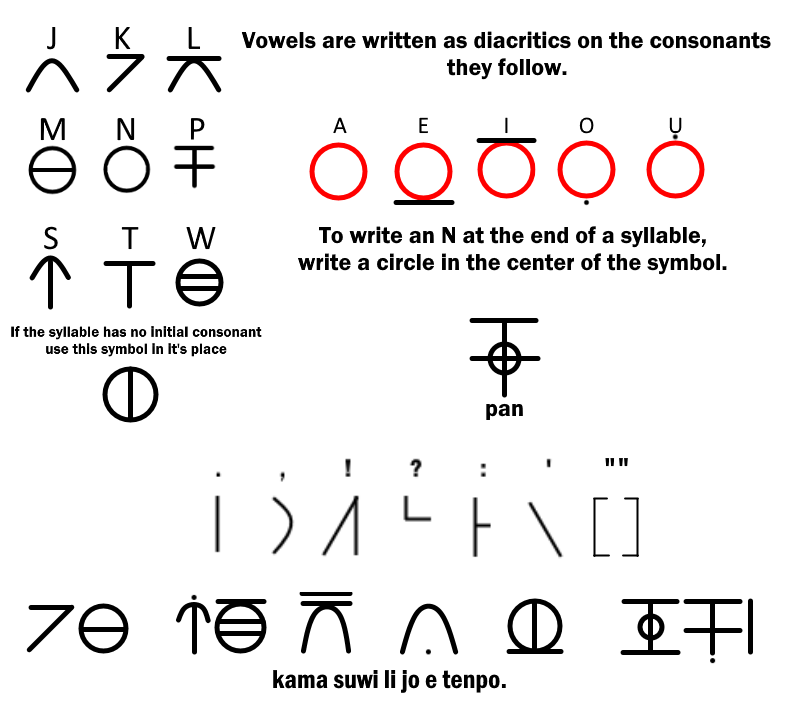
\includegraphics[scale=0.5]{sitelen_pona_pi_jan_Makuwe.png}

% 
%%%%%%%%%%%%%%%%%%%%%%%%%%%%%%%%%%%%%%%%%%%%%%%%%%%%%%%%%%%%%%%%%%%%%%%%%%
% eof

%
%%%%%%%%%%%%%%%%%%%%%%%%%%%%%%%%%%%%%%%%%%%%%%%%%%%%%%%%%%%%%%%%%%%%%%%%%%
\bibliography{toki-pona-lessons}
\bibliographystyle{plain}
\printindex
%%%%%%%%%%%%%%%%%%%%%%%%%%%%%%%%%%%%%%%%%%%%%%%%%%%%%%%%%%%%%%%%%%%%%%%%%%
\end{document}
%%%%%%%%%%%%%%%%%%%%%%%%%%%%%%%%%%%%%%%%%%%%%%%%%%%%%%%%%%%%%%%%%%%%%%%%%%
%%%%%%%%%%%%%%%%%%%%%%%%%%%%%%%%%%%%%%%%%%%%%%%%%%%%%%%%%%%%%%%%%%%%%%%%%%
%% eof
